\documentclass[twoside]{book}

% Packages required by doxygen
\usepackage{fixltx2e}
\usepackage{calc}
\usepackage{doxygen}
\usepackage[export]{adjustbox} % also loads graphicx
\usepackage{graphicx}
\usepackage[utf8]{inputenc}
\usepackage{makeidx}
\usepackage{multicol}
\usepackage{multirow}
\PassOptionsToPackage{warn}{textcomp}
\usepackage{textcomp}
\usepackage[nointegrals]{wasysym}
\usepackage[table]{xcolor}

% Font selection
\usepackage[T1]{fontenc}
\usepackage[scaled=.90]{helvet}
\usepackage{courier}
\usepackage{amssymb}
\usepackage{sectsty}
\renewcommand{\familydefault}{\sfdefault}
\allsectionsfont{%
  \fontseries{bc}\selectfont%
  \color{darkgray}%
}
\renewcommand{\DoxyLabelFont}{%
  \fontseries{bc}\selectfont%
  \color{darkgray}%
}
\newcommand{\+}{\discretionary{\mbox{\scriptsize$\hookleftarrow$}}{}{}}

% Page & text layout
\usepackage{geometry}
\geometry{%
  a4paper,%
  top=2.5cm,%
  bottom=2.5cm,%
  left=2.5cm,%
  right=2.5cm%
}
\tolerance=750
\hfuzz=15pt
\hbadness=750
\setlength{\emergencystretch}{15pt}
\setlength{\parindent}{0cm}
\setlength{\parskip}{3ex plus 2ex minus 2ex}
\makeatletter
\renewcommand{\paragraph}{%
  \@startsection{paragraph}{4}{0ex}{-1.0ex}{1.0ex}{%
    \normalfont\normalsize\bfseries\SS@parafont%
  }%
}
\renewcommand{\subparagraph}{%
  \@startsection{subparagraph}{5}{0ex}{-1.0ex}{1.0ex}{%
    \normalfont\normalsize\bfseries\SS@subparafont%
  }%
}
\makeatother

% Headers & footers
\usepackage{fancyhdr}
\pagestyle{fancyplain}
\fancyhead[LE]{\fancyplain{}{\bfseries\thepage}}
\fancyhead[CE]{\fancyplain{}{}}
\fancyhead[RE]{\fancyplain{}{\bfseries\leftmark}}
\fancyhead[LO]{\fancyplain{}{\bfseries\rightmark}}
\fancyhead[CO]{\fancyplain{}{}}
\fancyhead[RO]{\fancyplain{}{\bfseries\thepage}}
\fancyfoot[LE]{\fancyplain{}{}}
\fancyfoot[CE]{\fancyplain{}{}}
\fancyfoot[RE]{\fancyplain{}{\bfseries\scriptsize Generated by Doxygen }}
\fancyfoot[LO]{\fancyplain{}{\bfseries\scriptsize Generated by Doxygen }}
\fancyfoot[CO]{\fancyplain{}{}}
\fancyfoot[RO]{\fancyplain{}{}}
\renewcommand{\footrulewidth}{0.4pt}
\renewcommand{\chaptermark}[1]{%
  \markboth{#1}{}%
}
\renewcommand{\sectionmark}[1]{%
  \markright{\thesection\ #1}%
}

% Indices & bibliography
\usepackage{natbib}
\usepackage[titles]{tocloft}
\setcounter{tocdepth}{3}
\setcounter{secnumdepth}{5}
\makeindex

% Hyperlinks (required, but should be loaded last)
\usepackage{ifpdf}
\ifpdf
  \usepackage[pdftex,pagebackref=true]{hyperref}
\else
  \usepackage[ps2pdf,pagebackref=true]{hyperref}
\fi
\hypersetup{%
  colorlinks=true,%
  linkcolor=blue,%
  citecolor=blue,%
  unicode%
}

% Custom commands
\newcommand{\clearemptydoublepage}{%
  \newpage{\pagestyle{empty}\cleardoublepage}%
}

\usepackage{caption}
\captionsetup{labelsep=space,justification=centering,font={bf},singlelinecheck=off,skip=4pt,position=top}

%===== C O N T E N T S =====

\begin{document}

% Titlepage & ToC
\hypersetup{pageanchor=false,
             bookmarksnumbered=true,
             pdfencoding=unicode
            }
\pagenumbering{alph}
\begin{titlepage}
\vspace*{7cm}
\begin{center}%
{\Large My Project }\\
\vspace*{1cm}
{\large Generated by Doxygen 1.8.13}\\
\end{center}
\end{titlepage}
\clearemptydoublepage
\pagenumbering{roman}
\tableofcontents
\clearemptydoublepage
\pagenumbering{arabic}
\hypersetup{pageanchor=true}

%--- Begin generated contents ---
\chapter{Hierarchical Index}
\section{Class Hierarchy}
This inheritance list is sorted roughly, but not completely, alphabetically\+:\begin{DoxyCompactList}
\item \contentsline{section}{Player1}{\pageref{class_player1}}{}
\item Q\+Graphics\+Pixmap\+Item\begin{DoxyCompactList}
\item \contentsline{section}{Build\+Arrow\+Tower\+Icon}{\pageref{class_build_arrow_tower_icon}}{}
\item \contentsline{section}{Build\+Canon\+Tower\+Icon}{\pageref{class_build_canon_tower_icon}}{}
\item \contentsline{section}{Build\+Fire\+Tower\+Icon}{\pageref{class_build_fire_tower_icon}}{}
\item \contentsline{section}{Build\+Tower\+Icon}{\pageref{class_build_tower_icon}}{}
\item \contentsline{section}{Bullet}{\pageref{class_bullet}}{}
\item \contentsline{section}{Enemy}{\pageref{class_enemy}}{}
\item \contentsline{section}{Node}{\pageref{class_node}}{}
\begin{DoxyCompactList}
\item \contentsline{section}{Map}{\pageref{class_map}}{}
\end{DoxyCompactList}
\item \contentsline{section}{Reset\+Button}{\pageref{class_reset_button}}{}
\item \contentsline{section}{Sound}{\pageref{class_sound}}{}
\item \contentsline{section}{Spawn\+Eye\+Icon}{\pageref{class_spawn_eye_icon}}{}
\item \contentsline{section}{Tower}{\pageref{class_tower}}{}
\begin{DoxyCompactList}
\item \contentsline{section}{Arrow\+Tower}{\pageref{class_arrow_tower}}{}
\item \contentsline{section}{Canon\+Tower}{\pageref{class_canon_tower}}{}
\item \contentsline{section}{Fire\+Tower}{\pageref{class_fire_tower}}{}
\end{DoxyCompactList}
\end{DoxyCompactList}
\item Q\+Graphics\+Rect\+Item\begin{DoxyCompactList}
\item \contentsline{section}{Button}{\pageref{class_button}}{}
\end{DoxyCompactList}
\item Q\+Graphics\+View\begin{DoxyCompactList}
\item \contentsline{section}{Game}{\pageref{class_game}}{}
\end{DoxyCompactList}
\item Q\+Main\+Window\begin{DoxyCompactList}
\item \contentsline{section}{Main\+Window}{\pageref{class_main_window}}{}
\end{DoxyCompactList}
\item Q\+Object\begin{DoxyCompactList}
\item \contentsline{section}{Bullet}{\pageref{class_bullet}}{}
\item \contentsline{section}{Button}{\pageref{class_button}}{}
\item \contentsline{section}{Enemy}{\pageref{class_enemy}}{}
\item \contentsline{section}{Tower}{\pageref{class_tower}}{}
\item \contentsline{section}{U\+D\+P\+Socket}{\pageref{class_u_d_p_socket}}{}
\end{DoxyCompactList}
\item \contentsline{section}{U\+D\+P\+Class}{\pageref{class_u_d_p_class}}{}
\item \contentsline{section}{Waves}{\pageref{class_waves}}{}
\end{DoxyCompactList}

\chapter{Class Index}
\section{Class List}
Here are the classes, structs, unions and interfaces with brief descriptions\+:\begin{DoxyCompactList}
\item\contentsline{section}{\hyperlink{class_arrow_tower}{Arrow\+Tower} }{\pageref{class_arrow_tower}}{}
\item\contentsline{section}{\hyperlink{class_build_arrow_tower_icon}{Build\+Arrow\+Tower\+Icon} }{\pageref{class_build_arrow_tower_icon}}{}
\item\contentsline{section}{\hyperlink{class_build_canon_tower_icon}{Build\+Canon\+Tower\+Icon} }{\pageref{class_build_canon_tower_icon}}{}
\item\contentsline{section}{\hyperlink{class_build_fire_tower_icon}{Build\+Fire\+Tower\+Icon} }{\pageref{class_build_fire_tower_icon}}{}
\item\contentsline{section}{\hyperlink{class_build_tower_icon}{Build\+Tower\+Icon} }{\pageref{class_build_tower_icon}}{}
\item\contentsline{section}{\hyperlink{class_bullet}{Bullet} }{\pageref{class_bullet}}{}
\item\contentsline{section}{\hyperlink{class_button}{Button} }{\pageref{class_button}}{}
\item\contentsline{section}{\hyperlink{class_canon_tower}{Canon\+Tower} }{\pageref{class_canon_tower}}{}
\item\contentsline{section}{\hyperlink{class_enemy}{Enemy} }{\pageref{class_enemy}}{}
\item\contentsline{section}{\hyperlink{class_fire_tower}{Fire\+Tower} }{\pageref{class_fire_tower}}{}
\item\contentsline{section}{\hyperlink{class_game}{Game} }{\pageref{class_game}}{}
\item\contentsline{section}{\hyperlink{class_main_window}{Main\+Window} }{\pageref{class_main_window}}{}
\item\contentsline{section}{\hyperlink{class_map}{Map} }{\pageref{class_map}}{}
\item\contentsline{section}{\hyperlink{class_node}{Node} }{\pageref{class_node}}{}
\item\contentsline{section}{\hyperlink{class_player1}{Player1} }{\pageref{class_player1}}{}
\item\contentsline{section}{\hyperlink{class_reset_button}{Reset\+Button} }{\pageref{class_reset_button}}{}
\item\contentsline{section}{\hyperlink{class_sound}{Sound} }{\pageref{class_sound}}{}
\item\contentsline{section}{\hyperlink{class_spawn_eye_icon}{Spawn\+Eye\+Icon} }{\pageref{class_spawn_eye_icon}}{}
\item\contentsline{section}{\hyperlink{class_tower}{Tower} }{\pageref{class_tower}}{}
\item\contentsline{section}{\hyperlink{class_u_d_p_class}{U\+D\+P\+Class} }{\pageref{class_u_d_p_class}}{}
\item\contentsline{section}{\hyperlink{class_u_d_p_socket}{U\+D\+P\+Socket} }{\pageref{class_u_d_p_socket}}{}
\item\contentsline{section}{\hyperlink{class_waves}{Waves} }{\pageref{class_waves}}{}
\end{DoxyCompactList}

\chapter{File Index}
\section{File List}
Here is a list of all files with brief descriptions\+:\begin{DoxyCompactList}
\item\contentsline{section}{C\+:/\+Users/\+Fu\+Zzy/\+Dropbox/3de Jaar/\+Sem 1/\+R\+E\+I\+I313-\/\+C++ O\+O\+P/\+T\+D\+\_\+\+Game/\+Element\+\_\+\+T\+D/\hyperlink{arrowtower_8cpp}{arrowtower.\+cpp} }{\pageref{arrowtower_8cpp}}{}
\item\contentsline{section}{C\+:/\+Users/\+Fu\+Zzy/\+Dropbox/3de Jaar/\+Sem 1/\+R\+E\+I\+I313-\/\+C++ O\+O\+P/\+T\+D\+\_\+\+Game/\+Element\+\_\+\+T\+D/\hyperlink{arrowtower_8h}{arrowtower.\+h} }{\pageref{arrowtower_8h}}{}
\item\contentsline{section}{C\+:/\+Users/\+Fu\+Zzy/\+Dropbox/3de Jaar/\+Sem 1/\+R\+E\+I\+I313-\/\+C++ O\+O\+P/\+T\+D\+\_\+\+Game/\+Element\+\_\+\+T\+D/\hyperlink{buildarrowtowericon_8cpp}{buildarrowtowericon.\+cpp} }{\pageref{buildarrowtowericon_8cpp}}{}
\item\contentsline{section}{C\+:/\+Users/\+Fu\+Zzy/\+Dropbox/3de Jaar/\+Sem 1/\+R\+E\+I\+I313-\/\+C++ O\+O\+P/\+T\+D\+\_\+\+Game/\+Element\+\_\+\+T\+D/\hyperlink{buildarrowtowericon_8h}{buildarrowtowericon.\+h} }{\pageref{buildarrowtowericon_8h}}{}
\item\contentsline{section}{C\+:/\+Users/\+Fu\+Zzy/\+Dropbox/3de Jaar/\+Sem 1/\+R\+E\+I\+I313-\/\+C++ O\+O\+P/\+T\+D\+\_\+\+Game/\+Element\+\_\+\+T\+D/\hyperlink{buildcanontowericon_8cpp}{buildcanontowericon.\+cpp} }{\pageref{buildcanontowericon_8cpp}}{}
\item\contentsline{section}{C\+:/\+Users/\+Fu\+Zzy/\+Dropbox/3de Jaar/\+Sem 1/\+R\+E\+I\+I313-\/\+C++ O\+O\+P/\+T\+D\+\_\+\+Game/\+Element\+\_\+\+T\+D/\hyperlink{buildcanontowericon_8h}{buildcanontowericon.\+h} }{\pageref{buildcanontowericon_8h}}{}
\item\contentsline{section}{C\+:/\+Users/\+Fu\+Zzy/\+Dropbox/3de Jaar/\+Sem 1/\+R\+E\+I\+I313-\/\+C++ O\+O\+P/\+T\+D\+\_\+\+Game/\+Element\+\_\+\+T\+D/\hyperlink{buildfiretowericon_8cpp}{buildfiretowericon.\+cpp} }{\pageref{buildfiretowericon_8cpp}}{}
\item\contentsline{section}{C\+:/\+Users/\+Fu\+Zzy/\+Dropbox/3de Jaar/\+Sem 1/\+R\+E\+I\+I313-\/\+C++ O\+O\+P/\+T\+D\+\_\+\+Game/\+Element\+\_\+\+T\+D/\hyperlink{buildfiretowericon_8h}{buildfiretowericon.\+h} }{\pageref{buildfiretowericon_8h}}{}
\item\contentsline{section}{C\+:/\+Users/\+Fu\+Zzy/\+Dropbox/3de Jaar/\+Sem 1/\+R\+E\+I\+I313-\/\+C++ O\+O\+P/\+T\+D\+\_\+\+Game/\+Element\+\_\+\+T\+D/\hyperlink{buildtowericon_8cpp}{buildtowericon.\+cpp} }{\pageref{buildtowericon_8cpp}}{}
\item\contentsline{section}{C\+:/\+Users/\+Fu\+Zzy/\+Dropbox/3de Jaar/\+Sem 1/\+R\+E\+I\+I313-\/\+C++ O\+O\+P/\+T\+D\+\_\+\+Game/\+Element\+\_\+\+T\+D/\hyperlink{buildtowericon_8h}{buildtowericon.\+h} }{\pageref{buildtowericon_8h}}{}
\item\contentsline{section}{C\+:/\+Users/\+Fu\+Zzy/\+Dropbox/3de Jaar/\+Sem 1/\+R\+E\+I\+I313-\/\+C++ O\+O\+P/\+T\+D\+\_\+\+Game/\+Element\+\_\+\+T\+D/\hyperlink{bullet_8cpp}{bullet.\+cpp} }{\pageref{bullet_8cpp}}{}
\item\contentsline{section}{C\+:/\+Users/\+Fu\+Zzy/\+Dropbox/3de Jaar/\+Sem 1/\+R\+E\+I\+I313-\/\+C++ O\+O\+P/\+T\+D\+\_\+\+Game/\+Element\+\_\+\+T\+D/\hyperlink{bullet_8h}{bullet.\+h} }{\pageref{bullet_8h}}{}
\item\contentsline{section}{C\+:/\+Users/\+Fu\+Zzy/\+Dropbox/3de Jaar/\+Sem 1/\+R\+E\+I\+I313-\/\+C++ O\+O\+P/\+T\+D\+\_\+\+Game/\+Element\+\_\+\+T\+D/\hyperlink{button_8cpp}{button.\+cpp} }{\pageref{button_8cpp}}{}
\item\contentsline{section}{C\+:/\+Users/\+Fu\+Zzy/\+Dropbox/3de Jaar/\+Sem 1/\+R\+E\+I\+I313-\/\+C++ O\+O\+P/\+T\+D\+\_\+\+Game/\+Element\+\_\+\+T\+D/\hyperlink{button_8h}{button.\+h} }{\pageref{button_8h}}{}
\item\contentsline{section}{C\+:/\+Users/\+Fu\+Zzy/\+Dropbox/3de Jaar/\+Sem 1/\+R\+E\+I\+I313-\/\+C++ O\+O\+P/\+T\+D\+\_\+\+Game/\+Element\+\_\+\+T\+D/\hyperlink{canontower_8cpp}{canontower.\+cpp} }{\pageref{canontower_8cpp}}{}
\item\contentsline{section}{C\+:/\+Users/\+Fu\+Zzy/\+Dropbox/3de Jaar/\+Sem 1/\+R\+E\+I\+I313-\/\+C++ O\+O\+P/\+T\+D\+\_\+\+Game/\+Element\+\_\+\+T\+D/\hyperlink{canontower_8h}{canontower.\+h} }{\pageref{canontower_8h}}{}
\item\contentsline{section}{C\+:/\+Users/\+Fu\+Zzy/\+Dropbox/3de Jaar/\+Sem 1/\+R\+E\+I\+I313-\/\+C++ O\+O\+P/\+T\+D\+\_\+\+Game/\+Element\+\_\+\+T\+D/\hyperlink{enemy_8cpp}{enemy.\+cpp} }{\pageref{enemy_8cpp}}{}
\item\contentsline{section}{C\+:/\+Users/\+Fu\+Zzy/\+Dropbox/3de Jaar/\+Sem 1/\+R\+E\+I\+I313-\/\+C++ O\+O\+P/\+T\+D\+\_\+\+Game/\+Element\+\_\+\+T\+D/\hyperlink{enemy_8h}{enemy.\+h} }{\pageref{enemy_8h}}{}
\item\contentsline{section}{C\+:/\+Users/\+Fu\+Zzy/\+Dropbox/3de Jaar/\+Sem 1/\+R\+E\+I\+I313-\/\+C++ O\+O\+P/\+T\+D\+\_\+\+Game/\+Element\+\_\+\+T\+D/\hyperlink{firetower_8cpp}{firetower.\+cpp} }{\pageref{firetower_8cpp}}{}
\item\contentsline{section}{C\+:/\+Users/\+Fu\+Zzy/\+Dropbox/3de Jaar/\+Sem 1/\+R\+E\+I\+I313-\/\+C++ O\+O\+P/\+T\+D\+\_\+\+Game/\+Element\+\_\+\+T\+D/\hyperlink{firetower_8h}{firetower.\+h} }{\pageref{firetower_8h}}{}
\item\contentsline{section}{C\+:/\+Users/\+Fu\+Zzy/\+Dropbox/3de Jaar/\+Sem 1/\+R\+E\+I\+I313-\/\+C++ O\+O\+P/\+T\+D\+\_\+\+Game/\+Element\+\_\+\+T\+D/\hyperlink{game_8cpp}{game.\+cpp} }{\pageref{game_8cpp}}{}
\item\contentsline{section}{C\+:/\+Users/\+Fu\+Zzy/\+Dropbox/3de Jaar/\+Sem 1/\+R\+E\+I\+I313-\/\+C++ O\+O\+P/\+T\+D\+\_\+\+Game/\+Element\+\_\+\+T\+D/\hyperlink{game_8h}{game.\+h} }{\pageref{game_8h}}{}
\item\contentsline{section}{C\+:/\+Users/\+Fu\+Zzy/\+Dropbox/3de Jaar/\+Sem 1/\+R\+E\+I\+I313-\/\+C++ O\+O\+P/\+T\+D\+\_\+\+Game/\+Element\+\_\+\+T\+D/\hyperlink{main_8cpp}{main.\+cpp} }{\pageref{main_8cpp}}{}
\item\contentsline{section}{C\+:/\+Users/\+Fu\+Zzy/\+Dropbox/3de Jaar/\+Sem 1/\+R\+E\+I\+I313-\/\+C++ O\+O\+P/\+T\+D\+\_\+\+Game/\+Element\+\_\+\+T\+D/\hyperlink{mainwindow_8cpp}{mainwindow.\+cpp} }{\pageref{mainwindow_8cpp}}{}
\item\contentsline{section}{C\+:/\+Users/\+Fu\+Zzy/\+Dropbox/3de Jaar/\+Sem 1/\+R\+E\+I\+I313-\/\+C++ O\+O\+P/\+T\+D\+\_\+\+Game/\+Element\+\_\+\+T\+D/\hyperlink{mainwindow_8h}{mainwindow.\+h} }{\pageref{mainwindow_8h}}{}
\item\contentsline{section}{C\+:/\+Users/\+Fu\+Zzy/\+Dropbox/3de Jaar/\+Sem 1/\+R\+E\+I\+I313-\/\+C++ O\+O\+P/\+T\+D\+\_\+\+Game/\+Element\+\_\+\+T\+D/\hyperlink{map_8cpp}{map.\+cpp} }{\pageref{map_8cpp}}{}
\item\contentsline{section}{C\+:/\+Users/\+Fu\+Zzy/\+Dropbox/3de Jaar/\+Sem 1/\+R\+E\+I\+I313-\/\+C++ O\+O\+P/\+T\+D\+\_\+\+Game/\+Element\+\_\+\+T\+D/\hyperlink{map_8h}{map.\+h} }{\pageref{map_8h}}{}
\item\contentsline{section}{C\+:/\+Users/\+Fu\+Zzy/\+Dropbox/3de Jaar/\+Sem 1/\+R\+E\+I\+I313-\/\+C++ O\+O\+P/\+T\+D\+\_\+\+Game/\+Element\+\_\+\+T\+D/\hyperlink{node_8cpp}{node.\+cpp} }{\pageref{node_8cpp}}{}
\item\contentsline{section}{C\+:/\+Users/\+Fu\+Zzy/\+Dropbox/3de Jaar/\+Sem 1/\+R\+E\+I\+I313-\/\+C++ O\+O\+P/\+T\+D\+\_\+\+Game/\+Element\+\_\+\+T\+D/\hyperlink{node_8h}{node.\+h} }{\pageref{node_8h}}{}
\item\contentsline{section}{C\+:/\+Users/\+Fu\+Zzy/\+Dropbox/3de Jaar/\+Sem 1/\+R\+E\+I\+I313-\/\+C++ O\+O\+P/\+T\+D\+\_\+\+Game/\+Element\+\_\+\+T\+D/\hyperlink{player1_8cpp}{player1.\+cpp} }{\pageref{player1_8cpp}}{}
\item\contentsline{section}{C\+:/\+Users/\+Fu\+Zzy/\+Dropbox/3de Jaar/\+Sem 1/\+R\+E\+I\+I313-\/\+C++ O\+O\+P/\+T\+D\+\_\+\+Game/\+Element\+\_\+\+T\+D/\hyperlink{player1_8h}{player1.\+h} }{\pageref{player1_8h}}{}
\item\contentsline{section}{C\+:/\+Users/\+Fu\+Zzy/\+Dropbox/3de Jaar/\+Sem 1/\+R\+E\+I\+I313-\/\+C++ O\+O\+P/\+T\+D\+\_\+\+Game/\+Element\+\_\+\+T\+D/\hyperlink{resetbutton_8cpp}{resetbutton.\+cpp} }{\pageref{resetbutton_8cpp}}{}
\item\contentsline{section}{C\+:/\+Users/\+Fu\+Zzy/\+Dropbox/3de Jaar/\+Sem 1/\+R\+E\+I\+I313-\/\+C++ O\+O\+P/\+T\+D\+\_\+\+Game/\+Element\+\_\+\+T\+D/\hyperlink{resetbutton_8h}{resetbutton.\+h} }{\pageref{resetbutton_8h}}{}
\item\contentsline{section}{C\+:/\+Users/\+Fu\+Zzy/\+Dropbox/3de Jaar/\+Sem 1/\+R\+E\+I\+I313-\/\+C++ O\+O\+P/\+T\+D\+\_\+\+Game/\+Element\+\_\+\+T\+D/\hyperlink{sound_8cpp}{sound.\+cpp} }{\pageref{sound_8cpp}}{}
\item\contentsline{section}{C\+:/\+Users/\+Fu\+Zzy/\+Dropbox/3de Jaar/\+Sem 1/\+R\+E\+I\+I313-\/\+C++ O\+O\+P/\+T\+D\+\_\+\+Game/\+Element\+\_\+\+T\+D/\hyperlink{sound_8h}{sound.\+h} }{\pageref{sound_8h}}{}
\item\contentsline{section}{C\+:/\+Users/\+Fu\+Zzy/\+Dropbox/3de Jaar/\+Sem 1/\+R\+E\+I\+I313-\/\+C++ O\+O\+P/\+T\+D\+\_\+\+Game/\+Element\+\_\+\+T\+D/\hyperlink{spawneyeicon_8cpp}{spawneyeicon.\+cpp} }{\pageref{spawneyeicon_8cpp}}{}
\item\contentsline{section}{C\+:/\+Users/\+Fu\+Zzy/\+Dropbox/3de Jaar/\+Sem 1/\+R\+E\+I\+I313-\/\+C++ O\+O\+P/\+T\+D\+\_\+\+Game/\+Element\+\_\+\+T\+D/\hyperlink{spawneyeicon_8h}{spawneyeicon.\+h} }{\pageref{spawneyeicon_8h}}{}
\item\contentsline{section}{C\+:/\+Users/\+Fu\+Zzy/\+Dropbox/3de Jaar/\+Sem 1/\+R\+E\+I\+I313-\/\+C++ O\+O\+P/\+T\+D\+\_\+\+Game/\+Element\+\_\+\+T\+D/\hyperlink{tower_8cpp}{tower.\+cpp} }{\pageref{tower_8cpp}}{}
\item\contentsline{section}{C\+:/\+Users/\+Fu\+Zzy/\+Dropbox/3de Jaar/\+Sem 1/\+R\+E\+I\+I313-\/\+C++ O\+O\+P/\+T\+D\+\_\+\+Game/\+Element\+\_\+\+T\+D/\hyperlink{tower_8h}{tower.\+h} }{\pageref{tower_8h}}{}
\item\contentsline{section}{C\+:/\+Users/\+Fu\+Zzy/\+Dropbox/3de Jaar/\+Sem 1/\+R\+E\+I\+I313-\/\+C++ O\+O\+P/\+T\+D\+\_\+\+Game/\+Element\+\_\+\+T\+D/\hyperlink{udpclass_8cpp}{udpclass.\+cpp} }{\pageref{udpclass_8cpp}}{}
\item\contentsline{section}{C\+:/\+Users/\+Fu\+Zzy/\+Dropbox/3de Jaar/\+Sem 1/\+R\+E\+I\+I313-\/\+C++ O\+O\+P/\+T\+D\+\_\+\+Game/\+Element\+\_\+\+T\+D/\hyperlink{udpclass_8h}{udpclass.\+h} }{\pageref{udpclass_8h}}{}
\item\contentsline{section}{C\+:/\+Users/\+Fu\+Zzy/\+Dropbox/3de Jaar/\+Sem 1/\+R\+E\+I\+I313-\/\+C++ O\+O\+P/\+T\+D\+\_\+\+Game/\+Element\+\_\+\+T\+D/\hyperlink{udpsocket_8cpp}{udpsocket.\+cpp} }{\pageref{udpsocket_8cpp}}{}
\item\contentsline{section}{C\+:/\+Users/\+Fu\+Zzy/\+Dropbox/3de Jaar/\+Sem 1/\+R\+E\+I\+I313-\/\+C++ O\+O\+P/\+T\+D\+\_\+\+Game/\+Element\+\_\+\+T\+D/\hyperlink{udpsocket_8h}{udpsocket.\+h} }{\pageref{udpsocket_8h}}{}
\item\contentsline{section}{C\+:/\+Users/\+Fu\+Zzy/\+Dropbox/3de Jaar/\+Sem 1/\+R\+E\+I\+I313-\/\+C++ O\+O\+P/\+T\+D\+\_\+\+Game/\+Element\+\_\+\+T\+D/\hyperlink{waves_8cpp}{waves.\+cpp} }{\pageref{waves_8cpp}}{}
\item\contentsline{section}{C\+:/\+Users/\+Fu\+Zzy/\+Dropbox/3de Jaar/\+Sem 1/\+R\+E\+I\+I313-\/\+C++ O\+O\+P/\+T\+D\+\_\+\+Game/\+Element\+\_\+\+T\+D/\hyperlink{waves_8h}{waves.\+h} }{\pageref{waves_8h}}{}
\end{DoxyCompactList}

\chapter{Class Documentation}
\hypertarget{class_arrow_tower}{}\section{Arrow\+Tower Class Reference}
\label{class_arrow_tower}\index{Arrow\+Tower@{Arrow\+Tower}}


{\ttfamily \#include $<$arrowtower.\+h$>$}

Inheritance diagram for Arrow\+Tower\+:\begin{figure}[H]
\begin{center}
\leavevmode
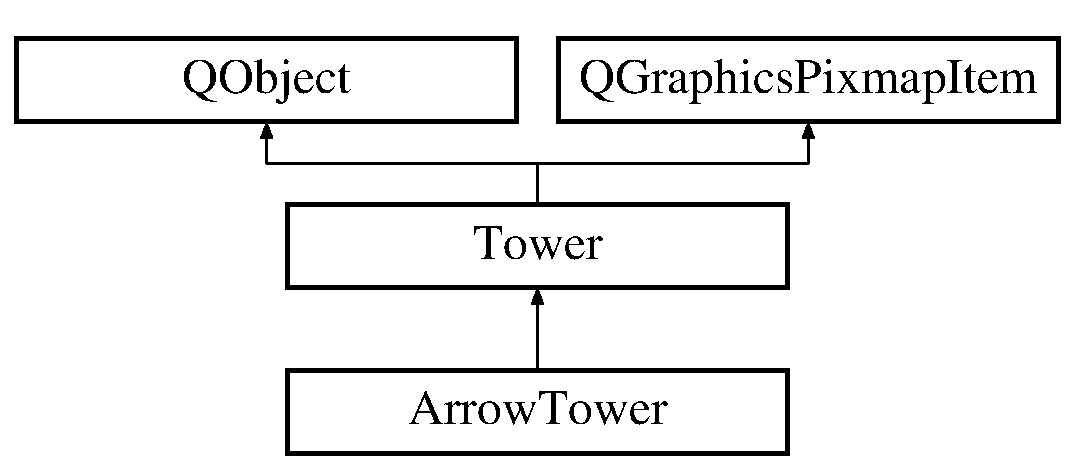
\includegraphics[height=3.000000cm]{class_arrow_tower}
\end{center}
\end{figure}
\subsection*{Public Slots}
\begin{DoxyCompactItemize}
\item 
void \hyperlink{class_arrow_tower_a0f2d63e9e3e3a8a1e6914711f3319df6}{aquire\+\_\+target} ()
\end{DoxyCompactItemize}
\subsection*{Public Member Functions}
\begin{DoxyCompactItemize}
\item 
\hyperlink{class_arrow_tower_a7b2c3a4465b810b204a46432266ba50e}{Arrow\+Tower} (Q\+Graphics\+Item $\ast$parent=0)
\item 
void \hyperlink{class_arrow_tower_ab4ed87128b5037a98640ab05e8721d88}{fire} ()
\item 
int \hyperlink{class_arrow_tower_a1ef82141056a39071f89d1c360728116}{get\+Cost\+Of\+Tower} ()
\item 
void \hyperlink{class_arrow_tower_afe62ccd8838829a0d7023d8eff079be2}{mouse\+Press\+Event} (Q\+Graphics\+Scene\+Mouse\+Event $\ast$event)
\item 
void \hyperlink{class_arrow_tower_a074c896d5ead33710d51e1c62a92862f}{mouse\+Double\+Click\+Event} (Q\+Graphics\+Scene\+Mouse\+Event $\ast$event)
\item 
void \hyperlink{class_arrow_tower_a7ac5bf2863d8a4c461d26a3a60dc62ab}{sell\+Tower} ()
\end{DoxyCompactItemize}
\subsection*{Public Attributes}
\begin{DoxyCompactItemize}
\item 
const int \hyperlink{class_arrow_tower_a5205aca3c7be32a30266f6e059857d90}{cost\+Of\+Tower} = 100
\end{DoxyCompactItemize}
\subsection*{Private Attributes}
\begin{DoxyCompactItemize}
\item 
Q\+Thread \hyperlink{class_arrow_tower_a3264fff2b7ceb29032942c88e80e2a65}{worker\+Thread}
\item 
int \hyperlink{class_arrow_tower_a3623752851bb010bb650ca63ed9dd26c}{tower\+Damage}
\end{DoxyCompactItemize}
\subsection*{Additional Inherited Members}


\subsection{Detailed Description}


Definition at line 9 of file arrowtower.\+h.



\subsection{Constructor \& Destructor Documentation}
\mbox{\Hypertarget{class_arrow_tower_a7b2c3a4465b810b204a46432266ba50e}\label{class_arrow_tower_a7b2c3a4465b810b204a46432266ba50e}} 
\index{Arrow\+Tower@{Arrow\+Tower}!Arrow\+Tower@{Arrow\+Tower}}
\index{Arrow\+Tower@{Arrow\+Tower}!Arrow\+Tower@{Arrow\+Tower}}
\subsubsection{\texorpdfstring{Arrow\+Tower()}{ArrowTower()}}
{\footnotesize\ttfamily Arrow\+Tower\+::\+Arrow\+Tower (\begin{DoxyParamCaption}\item[{Q\+Graphics\+Item $\ast$}]{parent = {\ttfamily 0} }\end{DoxyParamCaption})}



Definition at line 9 of file arrowtower.\+cpp.


\begin{DoxyCode}
10 \{
11     \textcolor{comment}{//set the graphics}
12     setPixmap(QPixmap(\textcolor{stringliteral}{":/images/images/Tower\_Arrow.png"}));
13     \textcolor{keywordtype}{int} w = pixmap().width();
14     \textcolor{keywordtype}{int} h = pixmap().height();
15     setOffset(-w/2,-h/1.25);
16 
17 
18     \textcolor{comment}{//connect timer to aaquire target}
19     QTimer * timer = \textcolor{keyword}{new} QTimer();
20     connect(timer,SIGNAL(timeout()),\textcolor{keyword}{this},SLOT(\hyperlink{class_arrow_tower_a0f2d63e9e3e3a8a1e6914711f3319df6}{aquire\_target}()));
21     timer->start(1500);
22 
23     \hyperlink{class_arrow_tower_a3623752851bb010bb650ca63ed9dd26c}{towerDamage} = 10;
24 \}
\end{DoxyCode}


\subsection{Member Function Documentation}
\mbox{\Hypertarget{class_arrow_tower_a0f2d63e9e3e3a8a1e6914711f3319df6}\label{class_arrow_tower_a0f2d63e9e3e3a8a1e6914711f3319df6}} 
\index{Arrow\+Tower@{Arrow\+Tower}!aquire\+\_\+target@{aquire\+\_\+target}}
\index{aquire\+\_\+target@{aquire\+\_\+target}!Arrow\+Tower@{Arrow\+Tower}}
\subsubsection{\texorpdfstring{aquire\+\_\+target}{aquire\_target}}
{\footnotesize\ttfamily void Arrow\+Tower\+::aquire\+\_\+target (\begin{DoxyParamCaption}{ }\end{DoxyParamCaption})\hspace{0.3cm}{\ttfamily [slot]}}



Definition at line 98 of file arrowtower.\+cpp.


\begin{DoxyCode}
99 \{
100     \hyperlink{class_tower_a6e0df1e43e746622967918aaf6f42dce}{Tower::aquire\_target}();
101 \}
\end{DoxyCode}
\mbox{\Hypertarget{class_arrow_tower_ab4ed87128b5037a98640ab05e8721d88}\label{class_arrow_tower_ab4ed87128b5037a98640ab05e8721d88}} 
\index{Arrow\+Tower@{Arrow\+Tower}!fire@{fire}}
\index{fire@{fire}!Arrow\+Tower@{Arrow\+Tower}}
\subsubsection{\texorpdfstring{fire()}{fire()}}
{\footnotesize\ttfamily void Arrow\+Tower\+::fire (\begin{DoxyParamCaption}{ }\end{DoxyParamCaption})\hspace{0.3cm}{\ttfamily [virtual]}}



Reimplemented from \hyperlink{class_tower_aa0c9c780f48cffacd3da6877f5d4fdc2}{Tower}.



Definition at line 26 of file arrowtower.\+cpp.


\begin{DoxyCode}
27 \{
28     \hyperlink{class_bullet}{Bullet} *bullet = \textcolor{keyword}{new} \hyperlink{class_bullet}{Bullet}();
29 
30     \textcolor{comment}{//place in new thread}
31 \textcolor{comment}{//    bullet->moveToThread(&workerThread);}
32 \textcolor{comment}{//    workerThread.start();}
33 
34     \textcolor{comment}{//set the graphics}
35     bullet->setPixmap(QPixmap(\textcolor{stringliteral}{":/images/images/Projectile\_Arrow-min.png"}));
36     \textcolor{comment}{//bullet->setScale(game->scalingfactor\_bullets);}
37 
38     \textcolor{comment}{//set the damage}
39     bullet->\hyperlink{class_bullet_a733d2ebbf9143c9ca68d3eb7e14121d0}{damage} = \hyperlink{class_arrow_tower_a3623752851bb010bb650ca63ed9dd26c}{towerDamage};
40 
41     \textcolor{keywordtype}{int} y\_pos = pixmap().height()*\hyperlink{arrowtower_8cpp_a58bdb5643d0814ac4e697a1564b79b70}{game}->\hyperlink{class_game_a6c1ca48f17f6934432d01bfa7f762a04}{scalingfactor\_towers}/1.25; \textcolor{comment}{//top of tower}
42 
43     bullet->setPos(x(), y()-y\_pos);
44 
45     QLineF ln(QPointF(x(), y()-y\_pos),\hyperlink{class_tower_a2b3e8ab90ccceed1fa3a667db80c2c06}{attack\_dest});
46     \textcolor{keywordtype}{int} angle = -1*ln.angle();
47 
48     bullet->setRotation(angle);
49     \hyperlink{arrowtower_8cpp_a58bdb5643d0814ac4e697a1564b79b70}{game}->\hyperlink{class_game_a8119e3b9a632906c6808fa294b46a92a}{scene}->addItem(bullet);
50 
51 \}
\end{DoxyCode}
\mbox{\Hypertarget{class_arrow_tower_a1ef82141056a39071f89d1c360728116}\label{class_arrow_tower_a1ef82141056a39071f89d1c360728116}} 
\index{Arrow\+Tower@{Arrow\+Tower}!get\+Cost\+Of\+Tower@{get\+Cost\+Of\+Tower}}
\index{get\+Cost\+Of\+Tower@{get\+Cost\+Of\+Tower}!Arrow\+Tower@{Arrow\+Tower}}
\subsubsection{\texorpdfstring{get\+Cost\+Of\+Tower()}{getCostOfTower()}}
{\footnotesize\ttfamily int Arrow\+Tower\+::get\+Cost\+Of\+Tower (\begin{DoxyParamCaption}{ }\end{DoxyParamCaption})\hspace{0.3cm}{\ttfamily [virtual]}}



Reimplemented from \hyperlink{class_tower_ae1d3f44d0149c8146ccf6b262a52ddad}{Tower}.



Definition at line 53 of file arrowtower.\+cpp.


\begin{DoxyCode}
54 \{
55     \textcolor{keywordflow}{return} \hyperlink{class_arrow_tower_a5205aca3c7be32a30266f6e059857d90}{costOfTower};
56 \}
\end{DoxyCode}
\mbox{\Hypertarget{class_arrow_tower_a074c896d5ead33710d51e1c62a92862f}\label{class_arrow_tower_a074c896d5ead33710d51e1c62a92862f}} 
\index{Arrow\+Tower@{Arrow\+Tower}!mouse\+Double\+Click\+Event@{mouse\+Double\+Click\+Event}}
\index{mouse\+Double\+Click\+Event@{mouse\+Double\+Click\+Event}!Arrow\+Tower@{Arrow\+Tower}}
\subsubsection{\texorpdfstring{mouse\+Double\+Click\+Event()}{mouseDoubleClickEvent()}}
{\footnotesize\ttfamily void Arrow\+Tower\+::mouse\+Double\+Click\+Event (\begin{DoxyParamCaption}\item[{Q\+Graphics\+Scene\+Mouse\+Event $\ast$}]{event }\end{DoxyParamCaption})}



Definition at line 75 of file arrowtower.\+cpp.


\begin{DoxyCode}
76 \{
77     \textcolor{comment}{//upgrade tower}
78     setPixmap(QPixmap(\textcolor{stringliteral}{":/images/images/Tower\_Arrow\_2.png"}));
79     \textcolor{keywordtype}{int} w = pixmap().width();
80     \textcolor{keywordtype}{int} h = pixmap().height();
81     setOffset(-w/2,-h/1.25);
82 
83     \textcolor{comment}{//upgrade damage}
84     \hyperlink{class_arrow_tower_a3623752851bb010bb650ca63ed9dd26c}{towerDamage} = 20;
85 
86     \textcolor{comment}{//update gold}
87     \hyperlink{arrowtower_8cpp_a58bdb5643d0814ac4e697a1564b79b70}{game}->\hyperlink{class_game_ad8a7cc146f99c7ec5b7c3c25d73f118c}{player1}->\hyperlink{class_player1_ab390478b345e443398bac442a04b675c}{Gold} += -\hyperlink{class_arrow_tower_a5205aca3c7be32a30266f6e059857d90}{costOfTower}/2;
88     \hyperlink{arrowtower_8cpp_a58bdb5643d0814ac4e697a1564b79b70}{game}->\hyperlink{class_game_a065998f7609f63e2987ede928359595a}{updateGold}();
89 
90 \}
\end{DoxyCode}
\mbox{\Hypertarget{class_arrow_tower_afe62ccd8838829a0d7023d8eff079be2}\label{class_arrow_tower_afe62ccd8838829a0d7023d8eff079be2}} 
\index{Arrow\+Tower@{Arrow\+Tower}!mouse\+Press\+Event@{mouse\+Press\+Event}}
\index{mouse\+Press\+Event@{mouse\+Press\+Event}!Arrow\+Tower@{Arrow\+Tower}}
\subsubsection{\texorpdfstring{mouse\+Press\+Event()}{mousePressEvent()}}
{\footnotesize\ttfamily void Arrow\+Tower\+::mouse\+Press\+Event (\begin{DoxyParamCaption}\item[{Q\+Graphics\+Scene\+Mouse\+Event $\ast$}]{event }\end{DoxyParamCaption})}



Definition at line 58 of file arrowtower.\+cpp.


\begin{DoxyCode}
59 \{
60 
61    qDebug() << \textcolor{stringliteral}{"Clicked Tower"};
62 
63    \textcolor{comment}{//right mouse sell}
64     \textcolor{keywordflow}{if} (event->button() == Qt::RightButton) \{
65         \hyperlink{class_arrow_tower_a7ac5bf2863d8a4c461d26a3a60dc62ab}{sellTower}();
66     \}
67     \textcolor{keywordflow}{else}
68     \{
69         \textcolor{comment}{//        QGraphicsView::mousePressEvent(event);}
70         \textcolor{keywordflow}{return};
71     \}
72 
73 \}
\end{DoxyCode}
\mbox{\Hypertarget{class_arrow_tower_a7ac5bf2863d8a4c461d26a3a60dc62ab}\label{class_arrow_tower_a7ac5bf2863d8a4c461d26a3a60dc62ab}} 
\index{Arrow\+Tower@{Arrow\+Tower}!sell\+Tower@{sell\+Tower}}
\index{sell\+Tower@{sell\+Tower}!Arrow\+Tower@{Arrow\+Tower}}
\subsubsection{\texorpdfstring{sell\+Tower()}{sellTower()}}
{\footnotesize\ttfamily void Arrow\+Tower\+::sell\+Tower (\begin{DoxyParamCaption}{ }\end{DoxyParamCaption})\hspace{0.3cm}{\ttfamily [virtual]}}



Reimplemented from \hyperlink{class_tower_a7736b1132e64e14a977e9e8c91c3338f}{Tower}.



Definition at line 92 of file arrowtower.\+cpp.


\begin{DoxyCode}
93 \{
94     qDebug() << \textcolor{stringliteral}{"sold arrow"};
95     \textcolor{comment}{//meh}
96 \}
\end{DoxyCode}


\subsection{Member Data Documentation}
\mbox{\Hypertarget{class_arrow_tower_a5205aca3c7be32a30266f6e059857d90}\label{class_arrow_tower_a5205aca3c7be32a30266f6e059857d90}} 
\index{Arrow\+Tower@{Arrow\+Tower}!cost\+Of\+Tower@{cost\+Of\+Tower}}
\index{cost\+Of\+Tower@{cost\+Of\+Tower}!Arrow\+Tower@{Arrow\+Tower}}
\subsubsection{\texorpdfstring{cost\+Of\+Tower}{costOfTower}}
{\footnotesize\ttfamily const int Arrow\+Tower\+::cost\+Of\+Tower = 100}



Definition at line 19 of file arrowtower.\+h.

\mbox{\Hypertarget{class_arrow_tower_a3623752851bb010bb650ca63ed9dd26c}\label{class_arrow_tower_a3623752851bb010bb650ca63ed9dd26c}} 
\index{Arrow\+Tower@{Arrow\+Tower}!tower\+Damage@{tower\+Damage}}
\index{tower\+Damage@{tower\+Damage}!Arrow\+Tower@{Arrow\+Tower}}
\subsubsection{\texorpdfstring{tower\+Damage}{towerDamage}}
{\footnotesize\ttfamily int Arrow\+Tower\+::tower\+Damage\hspace{0.3cm}{\ttfamily [private]}}



Definition at line 25 of file arrowtower.\+h.

\mbox{\Hypertarget{class_arrow_tower_a3264fff2b7ceb29032942c88e80e2a65}\label{class_arrow_tower_a3264fff2b7ceb29032942c88e80e2a65}} 
\index{Arrow\+Tower@{Arrow\+Tower}!worker\+Thread@{worker\+Thread}}
\index{worker\+Thread@{worker\+Thread}!Arrow\+Tower@{Arrow\+Tower}}
\subsubsection{\texorpdfstring{worker\+Thread}{workerThread}}
{\footnotesize\ttfamily Q\+Thread Arrow\+Tower\+::worker\+Thread\hspace{0.3cm}{\ttfamily [private]}}



Definition at line 24 of file arrowtower.\+h.



The documentation for this class was generated from the following files\+:\begin{DoxyCompactItemize}
\item 
C\+:/\+Users/\+Fu\+Zzy/\+Dropbox/3de Jaar/\+Sem 1/\+R\+E\+I\+I313-\/\+C++ O\+O\+P/\+T\+D\+\_\+\+Game/\+Element\+\_\+\+T\+D/\hyperlink{arrowtower_8h}{arrowtower.\+h}\item 
C\+:/\+Users/\+Fu\+Zzy/\+Dropbox/3de Jaar/\+Sem 1/\+R\+E\+I\+I313-\/\+C++ O\+O\+P/\+T\+D\+\_\+\+Game/\+Element\+\_\+\+T\+D/\hyperlink{arrowtower_8cpp}{arrowtower.\+cpp}\end{DoxyCompactItemize}

\hypertarget{class_build_arrow_tower_icon}{}\section{Build\+Arrow\+Tower\+Icon Class Reference}
\label{class_build_arrow_tower_icon}\index{Build\+Arrow\+Tower\+Icon@{Build\+Arrow\+Tower\+Icon}}


{\ttfamily \#include $<$buildarrowtowericon.\+h$>$}

Inheritance diagram for Build\+Arrow\+Tower\+Icon\+:\begin{figure}[H]
\begin{center}
\leavevmode
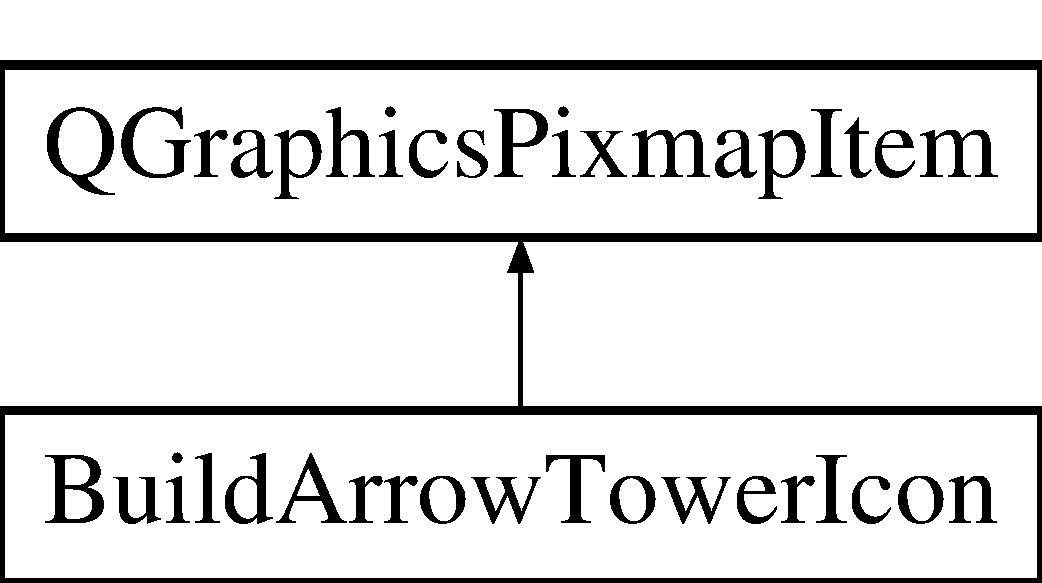
\includegraphics[height=2.000000cm]{class_build_arrow_tower_icon}
\end{center}
\end{figure}
\subsection*{Public Member Functions}
\begin{DoxyCompactItemize}
\item 
\hyperlink{class_build_arrow_tower_icon_af47deb48013cd6e384bc6713bd783f6e}{Build\+Arrow\+Tower\+Icon} (Q\+Graphics\+Item $\ast$parent=0)
\item 
void \hyperlink{class_build_arrow_tower_icon_ac2c2f51dd778437f191345b06751a785}{mouse\+Press\+Event} (Q\+Graphics\+Scene\+Mouse\+Event $\ast$event)
\item 
void \hyperlink{class_build_arrow_tower_icon_aad1a1a9846e6ccf27ca2becce40ce152}{hover\+Enter\+Event} (Q\+Graphics\+Scene\+Mouse\+Event $\ast$event)
\end{DoxyCompactItemize}


\subsection{Detailed Description}


Definition at line 7 of file buildarrowtowericon.\+h.



\subsection{Constructor \& Destructor Documentation}
\mbox{\Hypertarget{class_build_arrow_tower_icon_af47deb48013cd6e384bc6713bd783f6e}\label{class_build_arrow_tower_icon_af47deb48013cd6e384bc6713bd783f6e}} 
\index{Build\+Arrow\+Tower\+Icon@{Build\+Arrow\+Tower\+Icon}!Build\+Arrow\+Tower\+Icon@{Build\+Arrow\+Tower\+Icon}}
\index{Build\+Arrow\+Tower\+Icon@{Build\+Arrow\+Tower\+Icon}!Build\+Arrow\+Tower\+Icon@{Build\+Arrow\+Tower\+Icon}}
\subsubsection{\texorpdfstring{Build\+Arrow\+Tower\+Icon()}{BuildArrowTowerIcon()}}
{\footnotesize\ttfamily Build\+Arrow\+Tower\+Icon\+::\+Build\+Arrow\+Tower\+Icon (\begin{DoxyParamCaption}\item[{Q\+Graphics\+Item $\ast$}]{parent = {\ttfamily 0} }\end{DoxyParamCaption})}



Definition at line 8 of file buildarrowtowericon.\+cpp.


\begin{DoxyCode}
8                                                              : QGraphicsPixmapItem(parent)
9 \{
10     setPixmap(QPixmap(\textcolor{stringliteral}{":/images/images/Projectile\_Arrow.png"}));
11     \textcolor{keywordtype}{int} w = pixmap().width();
12     \textcolor{keywordtype}{int} h = pixmap().height();
13     setOffset(-w/2,-h/2);
14 
15     \textcolor{comment}{//allow hover events}
16     setAcceptHoverEvents(\textcolor{keyword}{true});
17 \}
\end{DoxyCode}


\subsection{Member Function Documentation}
\mbox{\Hypertarget{class_build_arrow_tower_icon_aad1a1a9846e6ccf27ca2becce40ce152}\label{class_build_arrow_tower_icon_aad1a1a9846e6ccf27ca2becce40ce152}} 
\index{Build\+Arrow\+Tower\+Icon@{Build\+Arrow\+Tower\+Icon}!hover\+Enter\+Event@{hover\+Enter\+Event}}
\index{hover\+Enter\+Event@{hover\+Enter\+Event}!Build\+Arrow\+Tower\+Icon@{Build\+Arrow\+Tower\+Icon}}
\subsubsection{\texorpdfstring{hover\+Enter\+Event()}{hoverEnterEvent()}}
{\footnotesize\ttfamily void Build\+Arrow\+Tower\+Icon\+::hover\+Enter\+Event (\begin{DoxyParamCaption}\item[{Q\+Graphics\+Scene\+Mouse\+Event $\ast$}]{event }\end{DoxyParamCaption})}



Definition at line 27 of file buildarrowtowericon.\+cpp.


\begin{DoxyCode}
28 \{
29     qDebug() << \textcolor{stringliteral}{"hovered"};
30 \}
\end{DoxyCode}
\mbox{\Hypertarget{class_build_arrow_tower_icon_ac2c2f51dd778437f191345b06751a785}\label{class_build_arrow_tower_icon_ac2c2f51dd778437f191345b06751a785}} 
\index{Build\+Arrow\+Tower\+Icon@{Build\+Arrow\+Tower\+Icon}!mouse\+Press\+Event@{mouse\+Press\+Event}}
\index{mouse\+Press\+Event@{mouse\+Press\+Event}!Build\+Arrow\+Tower\+Icon@{Build\+Arrow\+Tower\+Icon}}
\subsubsection{\texorpdfstring{mouse\+Press\+Event()}{mousePressEvent()}}
{\footnotesize\ttfamily void Build\+Arrow\+Tower\+Icon\+::mouse\+Press\+Event (\begin{DoxyParamCaption}\item[{Q\+Graphics\+Scene\+Mouse\+Event $\ast$}]{event }\end{DoxyParamCaption})}



Definition at line 19 of file buildarrowtowericon.\+cpp.


\begin{DoxyCode}
20 \{
21     \textcolor{keywordflow}{if} (!\hyperlink{buildarrowtowericon_8cpp_a58bdb5643d0814ac4e697a1564b79b70}{game}->\hyperlink{class_game_a5917b4e021a93be7666ebc2ef4529401}{building}) \{
22         \hyperlink{buildarrowtowericon_8cpp_a58bdb5643d0814ac4e697a1564b79b70}{game}->\hyperlink{class_game_a5917b4e021a93be7666ebc2ef4529401}{building} = \textcolor{keyword}{new} \hyperlink{class_arrow_tower}{ArrowTower}();
23         \hyperlink{buildarrowtowericon_8cpp_a58bdb5643d0814ac4e697a1564b79b70}{game}->\hyperlink{class_game_a7272e282812b8af0be83044db196dc6c}{setCursor}(QString(\textcolor{stringliteral}{":/images/images/Tower\_Arrow.png"}));
24     \}
25 \}
\end{DoxyCode}


The documentation for this class was generated from the following files\+:\begin{DoxyCompactItemize}
\item 
C\+:/\+Users/\+Fu\+Zzy/\+Dropbox/3de Jaar/\+Sem 1/\+R\+E\+I\+I313-\/\+C++ O\+O\+P/\+T\+D\+\_\+\+Game/\+Element\+\_\+\+T\+D/\hyperlink{buildarrowtowericon_8h}{buildarrowtowericon.\+h}\item 
C\+:/\+Users/\+Fu\+Zzy/\+Dropbox/3de Jaar/\+Sem 1/\+R\+E\+I\+I313-\/\+C++ O\+O\+P/\+T\+D\+\_\+\+Game/\+Element\+\_\+\+T\+D/\hyperlink{buildarrowtowericon_8cpp}{buildarrowtowericon.\+cpp}\end{DoxyCompactItemize}

\hypertarget{class_build_canon_tower_icon}{}\section{Build\+Canon\+Tower\+Icon Class Reference}
\label{class_build_canon_tower_icon}\index{Build\+Canon\+Tower\+Icon@{Build\+Canon\+Tower\+Icon}}


{\ttfamily \#include $<$buildcanontowericon.\+h$>$}

Inheritance diagram for Build\+Canon\+Tower\+Icon\+:\begin{figure}[H]
\begin{center}
\leavevmode
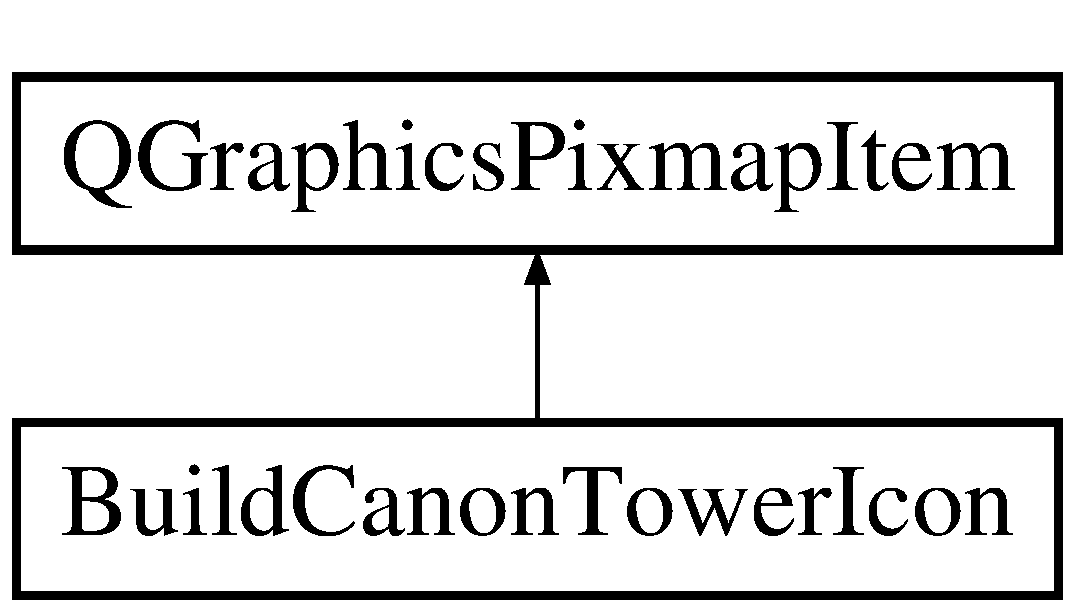
\includegraphics[height=2.000000cm]{class_build_canon_tower_icon}
\end{center}
\end{figure}
\subsection*{Public Member Functions}
\begin{DoxyCompactItemize}
\item 
\hyperlink{class_build_canon_tower_icon_aeb3649905f8558f236e051b269afcbf9}{Build\+Canon\+Tower\+Icon} (Q\+Graphics\+Item $\ast$parent=0)
\item 
void \hyperlink{class_build_canon_tower_icon_a81a8a1c5a2c312fb7facc4c9e423b6e5}{mouse\+Press\+Event} (Q\+Graphics\+Scene\+Mouse\+Event $\ast$event)
\end{DoxyCompactItemize}


\subsection{Detailed Description}


Definition at line 7 of file buildcanontowericon.\+h.



\subsection{Constructor \& Destructor Documentation}
\mbox{\Hypertarget{class_build_canon_tower_icon_aeb3649905f8558f236e051b269afcbf9}\label{class_build_canon_tower_icon_aeb3649905f8558f236e051b269afcbf9}} 
\index{Build\+Canon\+Tower\+Icon@{Build\+Canon\+Tower\+Icon}!Build\+Canon\+Tower\+Icon@{Build\+Canon\+Tower\+Icon}}
\index{Build\+Canon\+Tower\+Icon@{Build\+Canon\+Tower\+Icon}!Build\+Canon\+Tower\+Icon@{Build\+Canon\+Tower\+Icon}}
\subsubsection{\texorpdfstring{Build\+Canon\+Tower\+Icon()}{BuildCanonTowerIcon()}}
{\footnotesize\ttfamily Build\+Canon\+Tower\+Icon\+::\+Build\+Canon\+Tower\+Icon (\begin{DoxyParamCaption}\item[{Q\+Graphics\+Item $\ast$}]{parent = {\ttfamily 0} }\end{DoxyParamCaption})}



Definition at line 7 of file buildcanontowericon.\+cpp.


\begin{DoxyCode}
7                                                              : QGraphicsPixmapItem(parent)
8 \{
9     setPixmap(QPixmap(\textcolor{stringliteral}{":/images/images/Projectile\_Canon.png"}));
10     \textcolor{keywordtype}{int} w = pixmap().width();
11     \textcolor{keywordtype}{int} h = pixmap().height();
12     setOffset(-w/2,-h/2);
13 \}
\end{DoxyCode}


\subsection{Member Function Documentation}
\mbox{\Hypertarget{class_build_canon_tower_icon_a81a8a1c5a2c312fb7facc4c9e423b6e5}\label{class_build_canon_tower_icon_a81a8a1c5a2c312fb7facc4c9e423b6e5}} 
\index{Build\+Canon\+Tower\+Icon@{Build\+Canon\+Tower\+Icon}!mouse\+Press\+Event@{mouse\+Press\+Event}}
\index{mouse\+Press\+Event@{mouse\+Press\+Event}!Build\+Canon\+Tower\+Icon@{Build\+Canon\+Tower\+Icon}}
\subsubsection{\texorpdfstring{mouse\+Press\+Event()}{mousePressEvent()}}
{\footnotesize\ttfamily void Build\+Canon\+Tower\+Icon\+::mouse\+Press\+Event (\begin{DoxyParamCaption}\item[{Q\+Graphics\+Scene\+Mouse\+Event $\ast$}]{event }\end{DoxyParamCaption})}



Definition at line 15 of file buildcanontowericon.\+cpp.


\begin{DoxyCode}
16 \{
17     \textcolor{keywordflow}{if} (!\hyperlink{buildcanontowericon_8cpp_a58bdb5643d0814ac4e697a1564b79b70}{game}->\hyperlink{class_game_a5917b4e021a93be7666ebc2ef4529401}{building}) \{
18         \hyperlink{buildcanontowericon_8cpp_a58bdb5643d0814ac4e697a1564b79b70}{game}->\hyperlink{class_game_a5917b4e021a93be7666ebc2ef4529401}{building} = \textcolor{keyword}{new} \hyperlink{class_canon_tower}{CanonTower}();
19         \hyperlink{buildcanontowericon_8cpp_a58bdb5643d0814ac4e697a1564b79b70}{game}->\hyperlink{class_game_a7272e282812b8af0be83044db196dc6c}{setCursor}(QString(\textcolor{stringliteral}{":/images/images/Tower\_Canon.png"}));
20     \}
21 \}
\end{DoxyCode}


The documentation for this class was generated from the following files\+:\begin{DoxyCompactItemize}
\item 
C\+:/\+Users/\+Fu\+Zzy/\+Dropbox/3de Jaar/\+Sem 1/\+R\+E\+I\+I313-\/\+C++ O\+O\+P/\+T\+D\+\_\+\+Game/\+Element\+\_\+\+T\+D/\hyperlink{buildcanontowericon_8h}{buildcanontowericon.\+h}\item 
C\+:/\+Users/\+Fu\+Zzy/\+Dropbox/3de Jaar/\+Sem 1/\+R\+E\+I\+I313-\/\+C++ O\+O\+P/\+T\+D\+\_\+\+Game/\+Element\+\_\+\+T\+D/\hyperlink{buildcanontowericon_8cpp}{buildcanontowericon.\+cpp}\end{DoxyCompactItemize}

\hypertarget{class_build_fire_tower_icon}{}\section{Build\+Fire\+Tower\+Icon Class Reference}
\label{class_build_fire_tower_icon}\index{Build\+Fire\+Tower\+Icon@{Build\+Fire\+Tower\+Icon}}


{\ttfamily \#include $<$buildfiretowericon.\+h$>$}

Inheritance diagram for Build\+Fire\+Tower\+Icon\+:\begin{figure}[H]
\begin{center}
\leavevmode
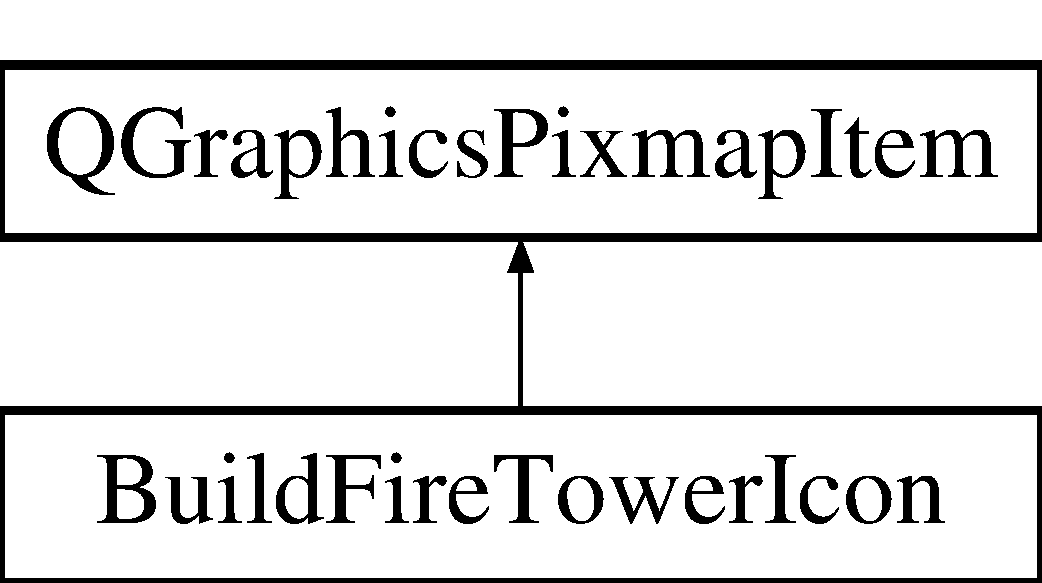
\includegraphics[height=2.000000cm]{class_build_fire_tower_icon}
\end{center}
\end{figure}
\subsection*{Public Member Functions}
\begin{DoxyCompactItemize}
\item 
\hyperlink{class_build_fire_tower_icon_a22891d990d32a248905f91348fe10f09}{Build\+Fire\+Tower\+Icon} (Q\+Graphics\+Item $\ast$parent=0)
\item 
void \hyperlink{class_build_fire_tower_icon_a878a78832a73bac6245ec0ae5bce5c60}{mouse\+Press\+Event} (Q\+Graphics\+Scene\+Mouse\+Event $\ast$event)
\end{DoxyCompactItemize}


\subsection{Detailed Description}


Definition at line 7 of file buildfiretowericon.\+h.



\subsection{Constructor \& Destructor Documentation}
\mbox{\Hypertarget{class_build_fire_tower_icon_a22891d990d32a248905f91348fe10f09}\label{class_build_fire_tower_icon_a22891d990d32a248905f91348fe10f09}} 
\index{Build\+Fire\+Tower\+Icon@{Build\+Fire\+Tower\+Icon}!Build\+Fire\+Tower\+Icon@{Build\+Fire\+Tower\+Icon}}
\index{Build\+Fire\+Tower\+Icon@{Build\+Fire\+Tower\+Icon}!Build\+Fire\+Tower\+Icon@{Build\+Fire\+Tower\+Icon}}
\subsubsection{\texorpdfstring{Build\+Fire\+Tower\+Icon()}{BuildFireTowerIcon()}}
{\footnotesize\ttfamily Build\+Fire\+Tower\+Icon\+::\+Build\+Fire\+Tower\+Icon (\begin{DoxyParamCaption}\item[{Q\+Graphics\+Item $\ast$}]{parent = {\ttfamily 0} }\end{DoxyParamCaption})}



Definition at line 7 of file buildfiretowericon.\+cpp.


\begin{DoxyCode}
7                                                            : QGraphicsPixmapItem(parent)
8 \{
9     setPixmap(QPixmap(\textcolor{stringliteral}{":/images/images/Projectile\_Fire.png"}));
10     \textcolor{keywordtype}{int} w = pixmap().width();
11     \textcolor{keywordtype}{int} h = pixmap().height();
12     setOffset(-w/2,-h/2);
13 \}
\end{DoxyCode}


\subsection{Member Function Documentation}
\mbox{\Hypertarget{class_build_fire_tower_icon_a878a78832a73bac6245ec0ae5bce5c60}\label{class_build_fire_tower_icon_a878a78832a73bac6245ec0ae5bce5c60}} 
\index{Build\+Fire\+Tower\+Icon@{Build\+Fire\+Tower\+Icon}!mouse\+Press\+Event@{mouse\+Press\+Event}}
\index{mouse\+Press\+Event@{mouse\+Press\+Event}!Build\+Fire\+Tower\+Icon@{Build\+Fire\+Tower\+Icon}}
\subsubsection{\texorpdfstring{mouse\+Press\+Event()}{mousePressEvent()}}
{\footnotesize\ttfamily void Build\+Fire\+Tower\+Icon\+::mouse\+Press\+Event (\begin{DoxyParamCaption}\item[{Q\+Graphics\+Scene\+Mouse\+Event $\ast$}]{event }\end{DoxyParamCaption})}



Definition at line 15 of file buildfiretowericon.\+cpp.


\begin{DoxyCode}
16 \{
17     \textcolor{keywordflow}{if} (!\hyperlink{buildfiretowericon_8cpp_a58bdb5643d0814ac4e697a1564b79b70}{game}->\hyperlink{class_game_a5917b4e021a93be7666ebc2ef4529401}{building}) \{
18         \hyperlink{buildfiretowericon_8cpp_a58bdb5643d0814ac4e697a1564b79b70}{game}->\hyperlink{class_game_a5917b4e021a93be7666ebc2ef4529401}{building} = \textcolor{keyword}{new} \hyperlink{class_fire_tower}{FireTower}();
19         \hyperlink{buildfiretowericon_8cpp_a58bdb5643d0814ac4e697a1564b79b70}{game}->\hyperlink{class_game_a7272e282812b8af0be83044db196dc6c}{setCursor}(QString(\textcolor{stringliteral}{":/images/images/Tower\_Fire.png"}));
20     \}
21 \}
\end{DoxyCode}


The documentation for this class was generated from the following files\+:\begin{DoxyCompactItemize}
\item 
C\+:/\+Users/\+Fu\+Zzy/\+Dropbox/3de Jaar/\+Sem 1/\+R\+E\+I\+I313-\/\+C++ O\+O\+P/\+T\+D\+\_\+\+Game/\+Element\+\_\+\+T\+D/\hyperlink{buildfiretowericon_8h}{buildfiretowericon.\+h}\item 
C\+:/\+Users/\+Fu\+Zzy/\+Dropbox/3de Jaar/\+Sem 1/\+R\+E\+I\+I313-\/\+C++ O\+O\+P/\+T\+D\+\_\+\+Game/\+Element\+\_\+\+T\+D/\hyperlink{buildfiretowericon_8cpp}{buildfiretowericon.\+cpp}\end{DoxyCompactItemize}

\hypertarget{class_build_tower_icon}{}\section{Build\+Tower\+Icon Class Reference}
\label{class_build_tower_icon}\index{Build\+Tower\+Icon@{Build\+Tower\+Icon}}


{\ttfamily \#include $<$buildtowericon.\+h$>$}

Inheritance diagram for Build\+Tower\+Icon\+:\begin{figure}[H]
\begin{center}
\leavevmode
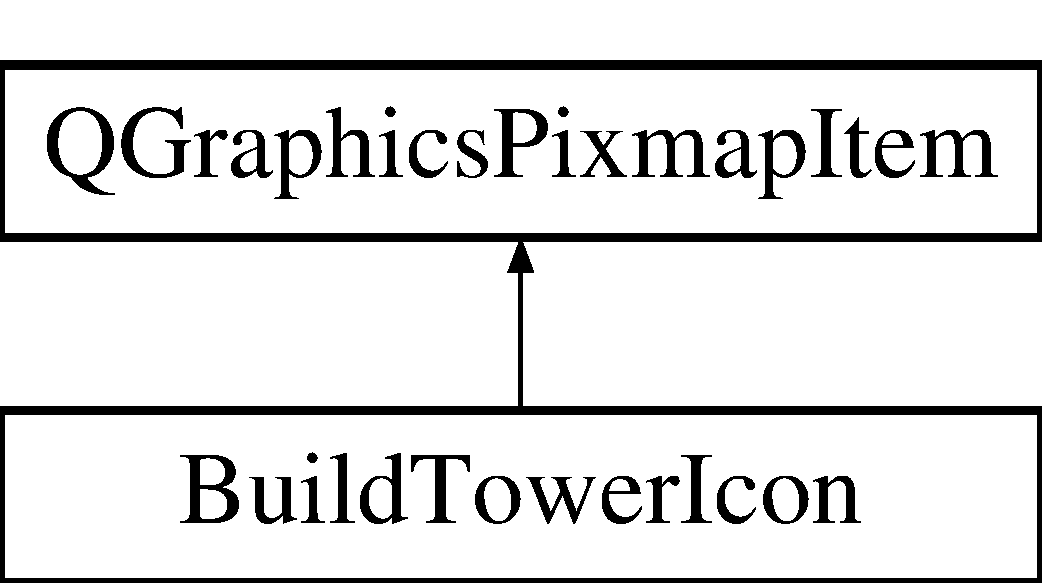
\includegraphics[height=2.000000cm]{class_build_tower_icon}
\end{center}
\end{figure}
\subsection*{Public Member Functions}
\begin{DoxyCompactItemize}
\item 
\hyperlink{class_build_tower_icon_a33a4d4435224d5ee68e6b1fa2a1dc5b4}{Build\+Tower\+Icon} (Q\+Graphics\+Item $\ast$parent=0)
\item 
void \hyperlink{class_build_tower_icon_a4232a6267dd0b252eb4bd58b36becc11}{mouse\+Press\+Event} (Q\+Graphics\+Scene\+Mouse\+Event $\ast$event)
\end{DoxyCompactItemize}


\subsection{Detailed Description}


Definition at line 7 of file buildtowericon.\+h.



\subsection{Constructor \& Destructor Documentation}
\mbox{\Hypertarget{class_build_tower_icon_a33a4d4435224d5ee68e6b1fa2a1dc5b4}\label{class_build_tower_icon_a33a4d4435224d5ee68e6b1fa2a1dc5b4}} 
\index{Build\+Tower\+Icon@{Build\+Tower\+Icon}!Build\+Tower\+Icon@{Build\+Tower\+Icon}}
\index{Build\+Tower\+Icon@{Build\+Tower\+Icon}!Build\+Tower\+Icon@{Build\+Tower\+Icon}}
\subsubsection{\texorpdfstring{Build\+Tower\+Icon()}{BuildTowerIcon()}}
{\footnotesize\ttfamily Build\+Tower\+Icon\+::\+Build\+Tower\+Icon (\begin{DoxyParamCaption}\item[{Q\+Graphics\+Item $\ast$}]{parent = {\ttfamily 0} }\end{DoxyParamCaption})}



Definition at line 6 of file buildtowericon.\+cpp.


\begin{DoxyCode}
6                                                    : QGraphicsPixmapItem(parent)
7 \{
8     setPixmap(QPixmap(\textcolor{stringliteral}{":/images/images/Projectile\_Arrow.png"}));
9 \}
\end{DoxyCode}


\subsection{Member Function Documentation}
\mbox{\Hypertarget{class_build_tower_icon_a4232a6267dd0b252eb4bd58b36becc11}\label{class_build_tower_icon_a4232a6267dd0b252eb4bd58b36becc11}} 
\index{Build\+Tower\+Icon@{Build\+Tower\+Icon}!mouse\+Press\+Event@{mouse\+Press\+Event}}
\index{mouse\+Press\+Event@{mouse\+Press\+Event}!Build\+Tower\+Icon@{Build\+Tower\+Icon}}
\subsubsection{\texorpdfstring{mouse\+Press\+Event()}{mousePressEvent()}}
{\footnotesize\ttfamily void Build\+Tower\+Icon\+::mouse\+Press\+Event (\begin{DoxyParamCaption}\item[{Q\+Graphics\+Scene\+Mouse\+Event $\ast$}]{event }\end{DoxyParamCaption})}



Definition at line 11 of file buildtowericon.\+cpp.


\begin{DoxyCode}
12 \{
13     \textcolor{keywordflow}{if} (!\hyperlink{buildtowericon_8cpp_a58bdb5643d0814ac4e697a1564b79b70}{game}->build) \{
14         \hyperlink{buildtowericon_8cpp_a58bdb5643d0814ac4e697a1564b79b70}{game}->build = \textcolor{keyword}{new} \hyperlink{class_tower}{Tower}();
15         \hyperlink{buildtowericon_8cpp_a58bdb5643d0814ac4e697a1564b79b70}{game}->\hyperlink{class_game_a7272e282812b8af0be83044db196dc6c}{setCursor}(QString(\textcolor{stringliteral}{":/images/images/Tower\_Arrow.png"}));
16     \}
17 \}
\end{DoxyCode}


The documentation for this class was generated from the following files\+:\begin{DoxyCompactItemize}
\item 
C\+:/\+Users/\+Fu\+Zzy/\+Dropbox/3de Jaar/\+Sem 1/\+R\+E\+I\+I313-\/\+C++ O\+O\+P/\+T\+D\+\_\+\+Game/\+Element\+\_\+\+T\+D/\hyperlink{buildtowericon_8h}{buildtowericon.\+h}\item 
C\+:/\+Users/\+Fu\+Zzy/\+Dropbox/3de Jaar/\+Sem 1/\+R\+E\+I\+I313-\/\+C++ O\+O\+P/\+T\+D\+\_\+\+Game/\+Element\+\_\+\+T\+D/\hyperlink{buildtowericon_8cpp}{buildtowericon.\+cpp}\end{DoxyCompactItemize}

\hypertarget{class_bullet}{}\section{Bullet Class Reference}
\label{class_bullet}\index{Bullet@{Bullet}}


{\ttfamily \#include $<$bullet.\+h$>$}

Inheritance diagram for Bullet\+:\begin{figure}[H]
\begin{center}
\leavevmode
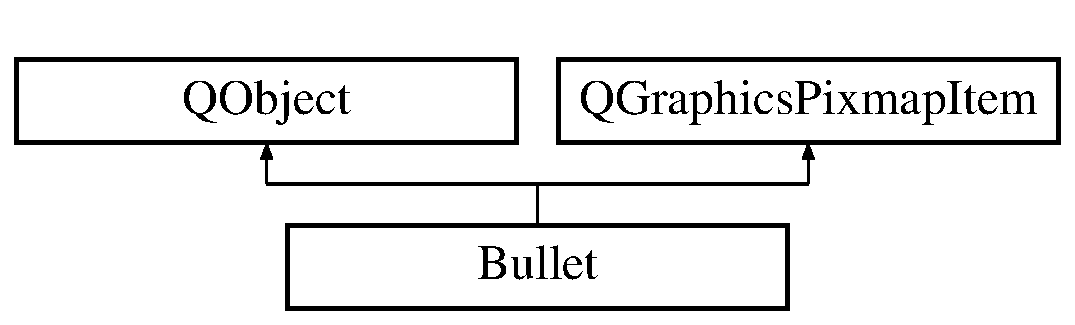
\includegraphics[height=2.000000cm]{class_bullet}
\end{center}
\end{figure}
\subsection*{Public Slots}
\begin{DoxyCompactItemize}
\item 
void \hyperlink{class_bullet_a6140db968c42c05e829e142f74f20b16}{move} ()
\item 
double \hyperlink{class_bullet_ada7a5f48649b2dc81ab1952cff51b6d9}{get\+Max\+Range} ()
\item 
double \hyperlink{class_bullet_ade9a9d09e42c002c7d30b65299194588}{get\+Distance\+Travelled} ()
\item 
void \hyperlink{class_bullet_a070852a34b912c9379338df18e32cf91}{set\+Max\+Range} (double rng)
\item 
void \hyperlink{class_bullet_ac1037d7a9f775b28bf1bc2727c018707}{set\+Distance\+Travelled} (double dist)
\end{DoxyCompactItemize}
\subsection*{Public Member Functions}
\begin{DoxyCompactItemize}
\item 
\hyperlink{class_bullet_a3d9f64399991ef430df460cac893b731}{Bullet} (Q\+Graphics\+Item $\ast$parent=0)
\item 
int \hyperlink{class_bullet_a682701fa7f9d4a9564dbcd6ed3f73588}{get\+Damage} ()
\end{DoxyCompactItemize}
\subsection*{Public Attributes}
\begin{DoxyCompactItemize}
\item 
int \hyperlink{class_bullet_a733d2ebbf9143c9ca68d3eb7e14121d0}{damage}
\end{DoxyCompactItemize}
\subsection*{Private Attributes}
\begin{DoxyCompactItemize}
\item 
double \hyperlink{class_bullet_ae7c4fadfcc22643cb271622fe8bb2eb0}{max\+Range}
\item 
double \hyperlink{class_bullet_afe194c1b7e495d0c17492396595202e1}{distance\+Travelled}
\end{DoxyCompactItemize}


\subsection{Detailed Description}


Definition at line 8 of file bullet.\+h.



\subsection{Constructor \& Destructor Documentation}
\mbox{\Hypertarget{class_bullet_a3d9f64399991ef430df460cac893b731}\label{class_bullet_a3d9f64399991ef430df460cac893b731}} 
\index{Bullet@{Bullet}!Bullet@{Bullet}}
\index{Bullet@{Bullet}!Bullet@{Bullet}}
\subsubsection{\texorpdfstring{Bullet()}{Bullet()}}
{\footnotesize\ttfamily Bullet\+::\+Bullet (\begin{DoxyParamCaption}\item[{Q\+Graphics\+Item $\ast$}]{parent = {\ttfamily 0} }\end{DoxyParamCaption})}



Definition at line 13 of file bullet.\+cpp.


\begin{DoxyCode}
14 \{
15     \textcolor{comment}{//set graphics}
16     setPixmap(QPixmap(\textcolor{stringliteral}{":/images/images/Projectile\_Arrow.png"}));
17 
18 
19     \textcolor{comment}{//connect timer to move}
20     \textcolor{comment}{//QTimer * move\_timer = new QTimer(this);}
21     connect(\hyperlink{bullet_8cpp_a58bdb5643d0814ac4e697a1564b79b70}{game}->\hyperlink{class_game_a4774e6e02e372dabcba313802800df5d}{bulletTimer}, SIGNAL(timeout()),\textcolor{keyword}{this},SLOT(\hyperlink{class_bullet_a6140db968c42c05e829e142f74f20b16}{move}()));
22     \textcolor{comment}{//move\_timer->start(50);}
23 
24     \textcolor{comment}{//initialize values}
25     \hyperlink{class_bullet_ae7c4fadfcc22643cb271622fe8bb2eb0}{maxRange} =250;
26     \hyperlink{class_bullet_afe194c1b7e495d0c17492396595202e1}{distanceTravelled} = 0;
27     \hyperlink{class_bullet_a733d2ebbf9143c9ca68d3eb7e14121d0}{damage} = 1;
28 \}
\end{DoxyCode}


\subsection{Member Function Documentation}
\mbox{\Hypertarget{class_bullet_a682701fa7f9d4a9564dbcd6ed3f73588}\label{class_bullet_a682701fa7f9d4a9564dbcd6ed3f73588}} 
\index{Bullet@{Bullet}!get\+Damage@{get\+Damage}}
\index{get\+Damage@{get\+Damage}!Bullet@{Bullet}}
\subsubsection{\texorpdfstring{get\+Damage()}{getDamage()}}
{\footnotesize\ttfamily int Bullet\+::get\+Damage (\begin{DoxyParamCaption}{ }\end{DoxyParamCaption})}



Definition at line 30 of file bullet.\+cpp.


\begin{DoxyCode}
31 \{
32     \textcolor{keywordflow}{return} \hyperlink{class_bullet_a733d2ebbf9143c9ca68d3eb7e14121d0}{damage};
33 \}
\end{DoxyCode}
\mbox{\Hypertarget{class_bullet_ade9a9d09e42c002c7d30b65299194588}\label{class_bullet_ade9a9d09e42c002c7d30b65299194588}} 
\index{Bullet@{Bullet}!get\+Distance\+Travelled@{get\+Distance\+Travelled}}
\index{get\+Distance\+Travelled@{get\+Distance\+Travelled}!Bullet@{Bullet}}
\subsubsection{\texorpdfstring{get\+Distance\+Travelled}{getDistanceTravelled}}
{\footnotesize\ttfamily double Bullet\+::get\+Distance\+Travelled (\begin{DoxyParamCaption}{ }\end{DoxyParamCaption})\hspace{0.3cm}{\ttfamily [slot]}}



Definition at line 86 of file bullet.\+cpp.


\begin{DoxyCode}
86                                    \{
87     \textcolor{keywordflow}{return} \hyperlink{class_bullet_afe194c1b7e495d0c17492396595202e1}{distanceTravelled};
88 \}
\end{DoxyCode}
\mbox{\Hypertarget{class_bullet_ada7a5f48649b2dc81ab1952cff51b6d9}\label{class_bullet_ada7a5f48649b2dc81ab1952cff51b6d9}} 
\index{Bullet@{Bullet}!get\+Max\+Range@{get\+Max\+Range}}
\index{get\+Max\+Range@{get\+Max\+Range}!Bullet@{Bullet}}
\subsubsection{\texorpdfstring{get\+Max\+Range}{getMaxRange}}
{\footnotesize\ttfamily double Bullet\+::get\+Max\+Range (\begin{DoxyParamCaption}{ }\end{DoxyParamCaption})\hspace{0.3cm}{\ttfamily [slot]}}



Definition at line 82 of file bullet.\+cpp.


\begin{DoxyCode}
82                           \{
83     \textcolor{keywordflow}{return} \hyperlink{class_bullet_ae7c4fadfcc22643cb271622fe8bb2eb0}{maxRange};
84 \}
\end{DoxyCode}
\mbox{\Hypertarget{class_bullet_a6140db968c42c05e829e142f74f20b16}\label{class_bullet_a6140db968c42c05e829e142f74f20b16}} 
\index{Bullet@{Bullet}!move@{move}}
\index{move@{move}!Bullet@{Bullet}}
\subsubsection{\texorpdfstring{move}{move}}
{\footnotesize\ttfamily void Bullet\+::move (\begin{DoxyParamCaption}{ }\end{DoxyParamCaption})\hspace{0.3cm}{\ttfamily [slot]}}



Definition at line 35 of file bullet.\+cpp.


\begin{DoxyCode}
36 \{
37     \textcolor{keywordtype}{int} STEP\_SIZE = 30;
38     \textcolor{keywordtype}{double} theta = rotation(); \textcolor{comment}{//degrees}
39 
40     \textcolor{keywordtype}{double} dy = STEP\_SIZE * qSin(qDegreesToRadians(theta));
41     \textcolor{keywordtype}{double} dx = STEP\_SIZE * qCos(qDegreesToRadians(theta));
42 
43     setPos(x()+dx, y()+dy);
44 
45     \hyperlink{class_bullet_afe194c1b7e495d0c17492396595202e1}{distanceTravelled} += STEP\_SIZE;
46 
47     \textcolor{comment}{//if collides with enemy}
48     QList<QGraphicsItem*> colliding\_items = collidingItems();
49         \textcolor{keywordflow}{for}(\textcolor{keywordtype}{int} i=0, n=colliding\_items.size(); i<n; i++)\{
50             \textcolor{keywordflow}{if}(\textcolor{keyword}{typeid}(*(colliding\_items[i]))==\textcolor{keyword}{typeid}(\hyperlink{class_enemy}{Enemy}))
51             \{
52              \hyperlink{class_enemy}{Enemy}* asEnemy = \textcolor{keyword}{dynamic\_cast<}\hyperlink{class_enemy}{Enemy}*\textcolor{keyword}{>}(colliding\_items[i]);
53              asEnemy->\hyperlink{class_enemy_ac7a5e3a071bcc4d67300cfae9446e0bd}{addDamage}(\hyperlink{class_bullet_a733d2ebbf9143c9ca68d3eb7e14121d0}{damage}); \textcolor{comment}{// CREATE addDamage function in Enemy}
54 
55              \textcolor{keywordflow}{if} (asEnemy->\hyperlink{class_enemy_aedd5e7bf8ef07ee97be433c853a10d8d}{health} <= 0) \{
56              \textcolor{comment}{//scene()->removeItem(asEnemy);}
57              \hyperlink{bullet_8cpp_a58bdb5643d0814ac4e697a1564b79b70}{game}->\hyperlink{class_game_ad8a7cc146f99c7ec5b7c3c25d73f118c}{player1}->\hyperlink{class_player1_ab390478b345e443398bac442a04b675c}{Gold} += asEnemy->\hyperlink{class_enemy_a8f007e72b954c077e5433a111def78c3}{loot};
58              \hyperlink{bullet_8cpp_a58bdb5643d0814ac4e697a1564b79b70}{game}->\hyperlink{class_game_a065998f7609f63e2987ede928359595a}{updateGold}();
59              qDebug() << \textcolor{stringliteral}{"You be dead son!"};
60              deleteLater();
61              \textcolor{comment}{//delete this;}
62              \textcolor{comment}{//delete asEnemy;}
63              asEnemy->deleteLater();
64              \hyperlink{bullet_8cpp_a58bdb5643d0814ac4e697a1564b79b70}{game}->\hyperlink{class_game_ab96914bfc1e59035233105abfb0787fe}{listOfEnemies}.removeOne(asEnemy);
65              \textcolor{keywordflow}{return};
66            \}
67 \textcolor{comment}{//             deleteLater();}
68 \textcolor{comment}{//             delete this;}
69         \}
70         \}
71 
72 
73     \textcolor{comment}{//if over max range}
74     \textcolor{keywordflow}{if} (\hyperlink{class_bullet_afe194c1b7e495d0c17492396595202e1}{distanceTravelled} >= \hyperlink{class_bullet_ae7c4fadfcc22643cb271622fe8bb2eb0}{maxRange}) \{
75         deleteLater();
76         \textcolor{comment}{//delete this;}
77     \}
78 
79 
80 \}
\end{DoxyCode}
\mbox{\Hypertarget{class_bullet_ac1037d7a9f775b28bf1bc2727c018707}\label{class_bullet_ac1037d7a9f775b28bf1bc2727c018707}} 
\index{Bullet@{Bullet}!set\+Distance\+Travelled@{set\+Distance\+Travelled}}
\index{set\+Distance\+Travelled@{set\+Distance\+Travelled}!Bullet@{Bullet}}
\subsubsection{\texorpdfstring{set\+Distance\+Travelled}{setDistanceTravelled}}
{\footnotesize\ttfamily void Bullet\+::set\+Distance\+Travelled (\begin{DoxyParamCaption}\item[{double}]{dist }\end{DoxyParamCaption})\hspace{0.3cm}{\ttfamily [slot]}}



Definition at line 94 of file bullet.\+cpp.


\begin{DoxyCode}
94                                             \{
95     \hyperlink{class_bullet_afe194c1b7e495d0c17492396595202e1}{distanceTravelled} = dist;
96 \}
\end{DoxyCode}
\mbox{\Hypertarget{class_bullet_a070852a34b912c9379338df18e32cf91}\label{class_bullet_a070852a34b912c9379338df18e32cf91}} 
\index{Bullet@{Bullet}!set\+Max\+Range@{set\+Max\+Range}}
\index{set\+Max\+Range@{set\+Max\+Range}!Bullet@{Bullet}}
\subsubsection{\texorpdfstring{set\+Max\+Range}{setMaxRange}}
{\footnotesize\ttfamily void Bullet\+::set\+Max\+Range (\begin{DoxyParamCaption}\item[{double}]{rng }\end{DoxyParamCaption})\hspace{0.3cm}{\ttfamily [slot]}}



Definition at line 90 of file bullet.\+cpp.


\begin{DoxyCode}
90                                   \{
91     \hyperlink{class_bullet_ae7c4fadfcc22643cb271622fe8bb2eb0}{maxRange} = rng;
92 \}
\end{DoxyCode}


\subsection{Member Data Documentation}
\mbox{\Hypertarget{class_bullet_a733d2ebbf9143c9ca68d3eb7e14121d0}\label{class_bullet_a733d2ebbf9143c9ca68d3eb7e14121d0}} 
\index{Bullet@{Bullet}!damage@{damage}}
\index{damage@{damage}!Bullet@{Bullet}}
\subsubsection{\texorpdfstring{damage}{damage}}
{\footnotesize\ttfamily int Bullet\+::damage}



Definition at line 12 of file bullet.\+h.

\mbox{\Hypertarget{class_bullet_afe194c1b7e495d0c17492396595202e1}\label{class_bullet_afe194c1b7e495d0c17492396595202e1}} 
\index{Bullet@{Bullet}!distance\+Travelled@{distance\+Travelled}}
\index{distance\+Travelled@{distance\+Travelled}!Bullet@{Bullet}}
\subsubsection{\texorpdfstring{distance\+Travelled}{distanceTravelled}}
{\footnotesize\ttfamily double Bullet\+::distance\+Travelled\hspace{0.3cm}{\ttfamily [private]}}



Definition at line 25 of file bullet.\+h.

\mbox{\Hypertarget{class_bullet_ae7c4fadfcc22643cb271622fe8bb2eb0}\label{class_bullet_ae7c4fadfcc22643cb271622fe8bb2eb0}} 
\index{Bullet@{Bullet}!max\+Range@{max\+Range}}
\index{max\+Range@{max\+Range}!Bullet@{Bullet}}
\subsubsection{\texorpdfstring{max\+Range}{maxRange}}
{\footnotesize\ttfamily double Bullet\+::max\+Range\hspace{0.3cm}{\ttfamily [private]}}



Definition at line 24 of file bullet.\+h.



The documentation for this class was generated from the following files\+:\begin{DoxyCompactItemize}
\item 
C\+:/\+Users/\+Fu\+Zzy/\+Dropbox/3de Jaar/\+Sem 1/\+R\+E\+I\+I313-\/\+C++ O\+O\+P/\+T\+D\+\_\+\+Game/\+Element\+\_\+\+T\+D/\hyperlink{bullet_8h}{bullet.\+h}\item 
C\+:/\+Users/\+Fu\+Zzy/\+Dropbox/3de Jaar/\+Sem 1/\+R\+E\+I\+I313-\/\+C++ O\+O\+P/\+T\+D\+\_\+\+Game/\+Element\+\_\+\+T\+D/\hyperlink{bullet_8cpp}{bullet.\+cpp}\end{DoxyCompactItemize}

\hypertarget{class_button}{}\section{Button Class Reference}
\label{class_button}\index{Button@{Button}}


{\ttfamily \#include $<$button.\+h$>$}

Inheritance diagram for Button\+:\begin{figure}[H]
\begin{center}
\leavevmode
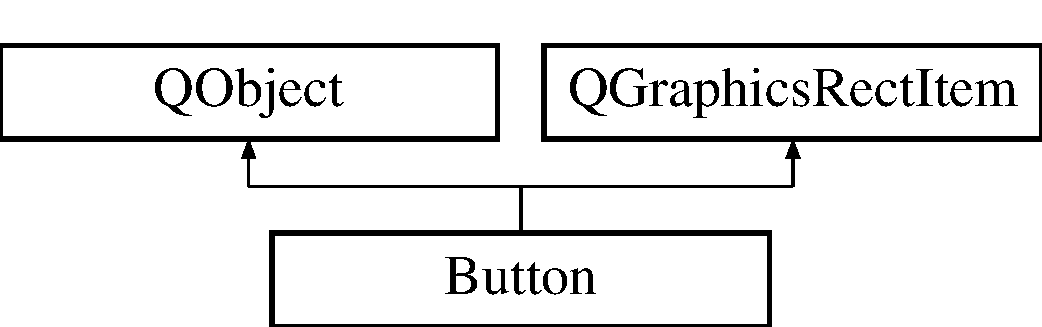
\includegraphics[height=2.000000cm]{class_button}
\end{center}
\end{figure}
\subsection*{Signals}
\begin{DoxyCompactItemize}
\item 
void \hyperlink{class_button_a9e7ab4152cb1e7e3beb7f2842f32670c}{clicked} ()
\end{DoxyCompactItemize}
\subsection*{Public Member Functions}
\begin{DoxyCompactItemize}
\item 
\hyperlink{class_button_a69976e5c00874a3807b642f249c1c776}{Button} (Q\+String name, Q\+Graphics\+Item $\ast$parent=N\+U\+LL)
\item 
void \hyperlink{class_button_a17d8eb0c904605b223bbc00c75655315}{mouse\+Press\+Event} (Q\+Graphics\+Scene\+Mouse\+Event $\ast$event)
\item 
void \hyperlink{class_button_a633a9684818bc5d300a622a00064f09c}{hover\+Enter\+Event} (Q\+Graphics\+Scene\+Hover\+Event $\ast$event)
\item 
void \hyperlink{class_button_ac7902a801be3eb542ce86e9c4cf4740d}{hoverleave\+Event} (Q\+Graphics\+Scene\+Hover\+Event $\ast$event)
\end{DoxyCompactItemize}
\subsection*{Private Attributes}
\begin{DoxyCompactItemize}
\item 
Q\+Graphics\+Text\+Item $\ast$ \hyperlink{class_button_a0d566bacc8c1befef9d09b839b6e76e6}{text}
\end{DoxyCompactItemize}


\subsection{Detailed Description}


Definition at line 7 of file button.\+h.



\subsection{Constructor \& Destructor Documentation}
\mbox{\Hypertarget{class_button_a69976e5c00874a3807b642f249c1c776}\label{class_button_a69976e5c00874a3807b642f249c1c776}} 
\index{Button@{Button}!Button@{Button}}
\index{Button@{Button}!Button@{Button}}
\subsubsection{\texorpdfstring{Button()}{Button()}}
{\footnotesize\ttfamily Button\+::\+Button (\begin{DoxyParamCaption}\item[{Q\+String}]{name,  }\item[{Q\+Graphics\+Item $\ast$}]{parent = {\ttfamily NULL} }\end{DoxyParamCaption})}



Definition at line 6 of file button.\+cpp.


\begin{DoxyCode}
6                                                  : QGraphicsRectItem(parent)
7 \{
8     \textcolor{comment}{//draw the rect}
9     setRect(0,0,200,50);
10     QBrush brush;
11     brush.setStyle(Qt::SolidPattern);
12     brush.setColor(Qt::darkCyan);
13     setBrush(brush);
14 
15     \textcolor{comment}{//draw the text}
16     \hyperlink{class_button_a0d566bacc8c1befef9d09b839b6e76e6}{text} = \textcolor{keyword}{new} QGraphicsTextItem(name, \textcolor{keyword}{this});
17     \textcolor{keywordtype}{int} xPos = rect().width()/2 - \hyperlink{class_button_a0d566bacc8c1befef9d09b839b6e76e6}{text}->boundingRect().width()/2;
18     \textcolor{keywordtype}{int} yPos = rect().height()/2 - \hyperlink{class_button_a0d566bacc8c1befef9d09b839b6e76e6}{text}->boundingRect().height()/2;
19     \hyperlink{class_button_a0d566bacc8c1befef9d09b839b6e76e6}{text}->setPos(xPos,yPos);
20 
21     \textcolor{comment}{//allow hover events}
22     setAcceptHoverEvents(\textcolor{keyword}{true});
23 
24 
25 \}
\end{DoxyCode}


\subsection{Member Function Documentation}
\mbox{\Hypertarget{class_button_a9e7ab4152cb1e7e3beb7f2842f32670c}\label{class_button_a9e7ab4152cb1e7e3beb7f2842f32670c}} 
\index{Button@{Button}!clicked@{clicked}}
\index{clicked@{clicked}!Button@{Button}}
\subsubsection{\texorpdfstring{clicked}{clicked}}
{\footnotesize\ttfamily void Button\+::clicked (\begin{DoxyParamCaption}{ }\end{DoxyParamCaption})\hspace{0.3cm}{\ttfamily [signal]}}

\mbox{\Hypertarget{class_button_a633a9684818bc5d300a622a00064f09c}\label{class_button_a633a9684818bc5d300a622a00064f09c}} 
\index{Button@{Button}!hover\+Enter\+Event@{hover\+Enter\+Event}}
\index{hover\+Enter\+Event@{hover\+Enter\+Event}!Button@{Button}}
\subsubsection{\texorpdfstring{hover\+Enter\+Event()}{hoverEnterEvent()}}
{\footnotesize\ttfamily void Button\+::hover\+Enter\+Event (\begin{DoxyParamCaption}\item[{Q\+Graphics\+Scene\+Hover\+Event $\ast$}]{event }\end{DoxyParamCaption})}



Definition at line 32 of file button.\+cpp.


\begin{DoxyCode}
33 \{
34     \textcolor{comment}{//change colour}
35     QBrush brush;
36     brush.setStyle(Qt::SolidPattern);
37     brush.setColor(Qt::cyan);
38     setBrush(brush);
39 \}
\end{DoxyCode}
\mbox{\Hypertarget{class_button_ac7902a801be3eb542ce86e9c4cf4740d}\label{class_button_ac7902a801be3eb542ce86e9c4cf4740d}} 
\index{Button@{Button}!hoverleave\+Event@{hoverleave\+Event}}
\index{hoverleave\+Event@{hoverleave\+Event}!Button@{Button}}
\subsubsection{\texorpdfstring{hoverleave\+Event()}{hoverleaveEvent()}}
{\footnotesize\ttfamily void Button\+::hoverleave\+Event (\begin{DoxyParamCaption}\item[{Q\+Graphics\+Scene\+Hover\+Event $\ast$}]{event }\end{DoxyParamCaption})}



Definition at line 41 of file button.\+cpp.


\begin{DoxyCode}
42 \{
43     \textcolor{comment}{//change colour back}
44     QBrush brush;
45     brush.setStyle(Qt::SolidPattern);
46     brush.setColor(Qt::darkCyan);
47     setBrush(brush);
48 \}
\end{DoxyCode}
\mbox{\Hypertarget{class_button_a17d8eb0c904605b223bbc00c75655315}\label{class_button_a17d8eb0c904605b223bbc00c75655315}} 
\index{Button@{Button}!mouse\+Press\+Event@{mouse\+Press\+Event}}
\index{mouse\+Press\+Event@{mouse\+Press\+Event}!Button@{Button}}
\subsubsection{\texorpdfstring{mouse\+Press\+Event()}{mousePressEvent()}}
{\footnotesize\ttfamily void Button\+::mouse\+Press\+Event (\begin{DoxyParamCaption}\item[{Q\+Graphics\+Scene\+Mouse\+Event $\ast$}]{event }\end{DoxyParamCaption})}



Definition at line 27 of file button.\+cpp.


\begin{DoxyCode}
28 \{
29     emit \hyperlink{class_button_a9e7ab4152cb1e7e3beb7f2842f32670c}{clicked}();
30 \}
\end{DoxyCode}


\subsection{Member Data Documentation}
\mbox{\Hypertarget{class_button_a0d566bacc8c1befef9d09b839b6e76e6}\label{class_button_a0d566bacc8c1befef9d09b839b6e76e6}} 
\index{Button@{Button}!text@{text}}
\index{text@{text}!Button@{Button}}
\subsubsection{\texorpdfstring{text}{text}}
{\footnotesize\ttfamily Q\+Graphics\+Text\+Item$\ast$ Button\+::text\hspace{0.3cm}{\ttfamily [private]}}



Definition at line 23 of file button.\+h.



The documentation for this class was generated from the following files\+:\begin{DoxyCompactItemize}
\item 
C\+:/\+Users/\+Fu\+Zzy/\+Dropbox/3de Jaar/\+Sem 1/\+R\+E\+I\+I313-\/\+C++ O\+O\+P/\+T\+D\+\_\+\+Game/\+Element\+\_\+\+T\+D/\hyperlink{button_8h}{button.\+h}\item 
C\+:/\+Users/\+Fu\+Zzy/\+Dropbox/3de Jaar/\+Sem 1/\+R\+E\+I\+I313-\/\+C++ O\+O\+P/\+T\+D\+\_\+\+Game/\+Element\+\_\+\+T\+D/\hyperlink{button_8cpp}{button.\+cpp}\end{DoxyCompactItemize}

\hypertarget{class_canon_tower}{}\section{Canon\+Tower Class Reference}
\label{class_canon_tower}\index{Canon\+Tower@{Canon\+Tower}}


{\ttfamily \#include $<$canontower.\+h$>$}

Inheritance diagram for Canon\+Tower\+:\begin{figure}[H]
\begin{center}
\leavevmode
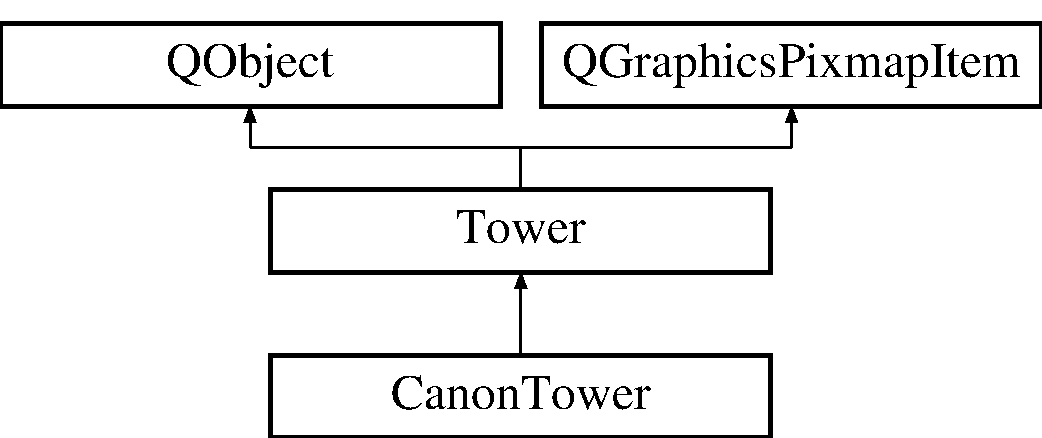
\includegraphics[height=3.000000cm]{class_canon_tower}
\end{center}
\end{figure}
\subsection*{Public Slots}
\begin{DoxyCompactItemize}
\item 
void \hyperlink{class_canon_tower_a02bacc0ba6efc6252b15c0daffbf87a9}{aquire\+\_\+target} ()
\end{DoxyCompactItemize}
\subsection*{Public Member Functions}
\begin{DoxyCompactItemize}
\item 
\hyperlink{class_canon_tower_a52a7edf2351dcf8646f25ff97c97cdf3}{Canon\+Tower} (Q\+Graphics\+Item $\ast$parent=0)
\item 
void \hyperlink{class_canon_tower_aa8d13cf8b8d530256b95746620e16234}{fire} ()
\item 
int \hyperlink{class_canon_tower_ac0e57d350da509e89e926afe950ab291}{get\+Cost\+Of\+Tower} ()
\item 
void \hyperlink{class_canon_tower_a15edd7ff8846e44faaca6ab5e7b183dc}{mouse\+Press\+Event} (Q\+Graphics\+Scene\+Mouse\+Event $\ast$event)
\item 
void \hyperlink{class_canon_tower_ac4956cf0bb621db0874403551eaf1eb1}{mouse\+Double\+Click\+Event} (Q\+Graphics\+Scene\+Mouse\+Event $\ast$event)
\item 
void \hyperlink{class_canon_tower_a5bfc0567c8907e8a6ddf4722f6783cd0}{sell\+Tower} ()
\end{DoxyCompactItemize}
\subsection*{Public Attributes}
\begin{DoxyCompactItemize}
\item 
const int \hyperlink{class_canon_tower_a545089ae31859c4bf0e46316c637383b}{cost\+Of\+Tower} = 200
\end{DoxyCompactItemize}
\subsection*{Private Attributes}
\begin{DoxyCompactItemize}
\item 
int \hyperlink{class_canon_tower_a26ea42f5a200246080dfba01340f057b}{tower\+Damage}
\end{DoxyCompactItemize}
\subsection*{Additional Inherited Members}


\subsection{Detailed Description}


Definition at line 7 of file canontower.\+h.



\subsection{Constructor \& Destructor Documentation}
\mbox{\Hypertarget{class_canon_tower_a52a7edf2351dcf8646f25ff97c97cdf3}\label{class_canon_tower_a52a7edf2351dcf8646f25ff97c97cdf3}} 
\index{Canon\+Tower@{Canon\+Tower}!Canon\+Tower@{Canon\+Tower}}
\index{Canon\+Tower@{Canon\+Tower}!Canon\+Tower@{Canon\+Tower}}
\subsubsection{\texorpdfstring{Canon\+Tower()}{CanonTower()}}
{\footnotesize\ttfamily Canon\+Tower\+::\+Canon\+Tower (\begin{DoxyParamCaption}\item[{Q\+Graphics\+Item $\ast$}]{parent = {\ttfamily 0} }\end{DoxyParamCaption})}



Definition at line 9 of file canontower.\+cpp.


\begin{DoxyCode}
10 \{
11     \textcolor{comment}{//set graphics}
12     setPixmap(QPixmap(\textcolor{stringliteral}{":/images/images/Tower\_Canon.png"}));
13     \textcolor{keywordtype}{int} w = pixmap().width();
14     \textcolor{keywordtype}{int} h = pixmap().height();
15     setOffset(-w/2,-h/1.25);
16 
17     \textcolor{comment}{//connect timer to aaquire target}
18     QTimer * timer = \textcolor{keyword}{new} QTimer();
19     connect(timer,SIGNAL(timeout()),\textcolor{keyword}{this},SLOT(\hyperlink{class_canon_tower_a02bacc0ba6efc6252b15c0daffbf87a9}{aquire\_target}()));
20     timer->start(2000);
21 \}
\end{DoxyCode}


\subsection{Member Function Documentation}
\mbox{\Hypertarget{class_canon_tower_a02bacc0ba6efc6252b15c0daffbf87a9}\label{class_canon_tower_a02bacc0ba6efc6252b15c0daffbf87a9}} 
\index{Canon\+Tower@{Canon\+Tower}!aquire\+\_\+target@{aquire\+\_\+target}}
\index{aquire\+\_\+target@{aquire\+\_\+target}!Canon\+Tower@{Canon\+Tower}}
\subsubsection{\texorpdfstring{aquire\+\_\+target}{aquire\_target}}
{\footnotesize\ttfamily void Canon\+Tower\+::aquire\+\_\+target (\begin{DoxyParamCaption}{ }\end{DoxyParamCaption})\hspace{0.3cm}{\ttfamily [slot]}}



Definition at line 53 of file canontower.\+cpp.


\begin{DoxyCode}
54 \{
55     \hyperlink{class_tower_a6e0df1e43e746622967918aaf6f42dce}{Tower::aquire\_target}();
56 \}
\end{DoxyCode}
\mbox{\Hypertarget{class_canon_tower_aa8d13cf8b8d530256b95746620e16234}\label{class_canon_tower_aa8d13cf8b8d530256b95746620e16234}} 
\index{Canon\+Tower@{Canon\+Tower}!fire@{fire}}
\index{fire@{fire}!Canon\+Tower@{Canon\+Tower}}
\subsubsection{\texorpdfstring{fire()}{fire()}}
{\footnotesize\ttfamily void Canon\+Tower\+::fire (\begin{DoxyParamCaption}{ }\end{DoxyParamCaption})\hspace{0.3cm}{\ttfamily [virtual]}}



Reimplemented from \hyperlink{class_tower_aa0c9c780f48cffacd3da6877f5d4fdc2}{Tower}.



Definition at line 23 of file canontower.\+cpp.


\begin{DoxyCode}
24 \{
25     \textcolor{comment}{//create the bullets}
26     \hyperlink{class_bullet}{Bullet} *bullet = \textcolor{keyword}{new} \hyperlink{class_bullet}{Bullet}();
27 
28     \textcolor{comment}{//set the graphics}
29     bullet->setPixmap(QPixmap(\textcolor{stringliteral}{":/images/images/Projectile\_Canon-min.png"}));
30     \textcolor{comment}{//bullet->setScale(game->scalingfactor\_bullets);}
31 
32     \textcolor{comment}{//set the damage}
33     bullet->\hyperlink{class_bullet_a733d2ebbf9143c9ca68d3eb7e14121d0}{damage} = 30;
34 
35     \textcolor{keywordtype}{int} y\_pos = pixmap().height()*\hyperlink{canontower_8cpp_a58bdb5643d0814ac4e697a1564b79b70}{game}->\hyperlink{class_game_a6c1ca48f17f6934432d01bfa7f762a04}{scalingfactor\_towers}/1.25;
36 
37     bullet->setPos(x(), y()-y\_pos);
38 
39     QLineF ln(QPointF(x(), y()-y\_pos),\hyperlink{class_tower_a2b3e8ab90ccceed1fa3a667db80c2c06}{attack\_dest});
40     \textcolor{keywordtype}{int} angle = -1*ln.angle();
41 
42     bullet->setRotation(angle);
43 
44     \hyperlink{canontower_8cpp_a58bdb5643d0814ac4e697a1564b79b70}{game}->\hyperlink{class_game_a8119e3b9a632906c6808fa294b46a92a}{scene}->addItem(bullet);
45 
46 \}
\end{DoxyCode}
\mbox{\Hypertarget{class_canon_tower_ac0e57d350da509e89e926afe950ab291}\label{class_canon_tower_ac0e57d350da509e89e926afe950ab291}} 
\index{Canon\+Tower@{Canon\+Tower}!get\+Cost\+Of\+Tower@{get\+Cost\+Of\+Tower}}
\index{get\+Cost\+Of\+Tower@{get\+Cost\+Of\+Tower}!Canon\+Tower@{Canon\+Tower}}
\subsubsection{\texorpdfstring{get\+Cost\+Of\+Tower()}{getCostOfTower()}}
{\footnotesize\ttfamily int Canon\+Tower\+::get\+Cost\+Of\+Tower (\begin{DoxyParamCaption}{ }\end{DoxyParamCaption})\hspace{0.3cm}{\ttfamily [virtual]}}



Reimplemented from \hyperlink{class_tower_ae1d3f44d0149c8146ccf6b262a52ddad}{Tower}.



Definition at line 48 of file canontower.\+cpp.


\begin{DoxyCode}
49 \{
50     \textcolor{keywordflow}{return} \hyperlink{class_canon_tower_a545089ae31859c4bf0e46316c637383b}{costOfTower};
51 \}
\end{DoxyCode}
\mbox{\Hypertarget{class_canon_tower_ac4956cf0bb621db0874403551eaf1eb1}\label{class_canon_tower_ac4956cf0bb621db0874403551eaf1eb1}} 
\index{Canon\+Tower@{Canon\+Tower}!mouse\+Double\+Click\+Event@{mouse\+Double\+Click\+Event}}
\index{mouse\+Double\+Click\+Event@{mouse\+Double\+Click\+Event}!Canon\+Tower@{Canon\+Tower}}
\subsubsection{\texorpdfstring{mouse\+Double\+Click\+Event()}{mouseDoubleClickEvent()}}
{\footnotesize\ttfamily void Canon\+Tower\+::mouse\+Double\+Click\+Event (\begin{DoxyParamCaption}\item[{Q\+Graphics\+Scene\+Mouse\+Event $\ast$}]{event }\end{DoxyParamCaption})}



Definition at line 75 of file canontower.\+cpp.


\begin{DoxyCode}
76 \{
77     \textcolor{comment}{//upgrade tower}
78     setPixmap(QPixmap(\textcolor{stringliteral}{":/images/images/Tower\_Canon\_2.png"}));
79     \textcolor{keywordtype}{int} w = pixmap().width();
80     \textcolor{keywordtype}{int} h = pixmap().height();
81     setOffset(-w/2,-h/1.25);
82 
83     \textcolor{comment}{//upgrade damage}
84     \hyperlink{class_canon_tower_a26ea42f5a200246080dfba01340f057b}{towerDamage} = 60;
85 
86     \textcolor{comment}{//update gold}
87     \hyperlink{canontower_8cpp_a58bdb5643d0814ac4e697a1564b79b70}{game}->\hyperlink{class_game_ad8a7cc146f99c7ec5b7c3c25d73f118c}{player1}->\hyperlink{class_player1_ab390478b345e443398bac442a04b675c}{Gold} += -\hyperlink{class_canon_tower_a545089ae31859c4bf0e46316c637383b}{costOfTower}/2;
88     \hyperlink{canontower_8cpp_a58bdb5643d0814ac4e697a1564b79b70}{game}->\hyperlink{class_game_a065998f7609f63e2987ede928359595a}{updateGold}();
89 
90 \}
\end{DoxyCode}
\mbox{\Hypertarget{class_canon_tower_a15edd7ff8846e44faaca6ab5e7b183dc}\label{class_canon_tower_a15edd7ff8846e44faaca6ab5e7b183dc}} 
\index{Canon\+Tower@{Canon\+Tower}!mouse\+Press\+Event@{mouse\+Press\+Event}}
\index{mouse\+Press\+Event@{mouse\+Press\+Event}!Canon\+Tower@{Canon\+Tower}}
\subsubsection{\texorpdfstring{mouse\+Press\+Event()}{mousePressEvent()}}
{\footnotesize\ttfamily void Canon\+Tower\+::mouse\+Press\+Event (\begin{DoxyParamCaption}\item[{Q\+Graphics\+Scene\+Mouse\+Event $\ast$}]{event }\end{DoxyParamCaption})}



Definition at line 58 of file canontower.\+cpp.


\begin{DoxyCode}
59 \{
60 
61    qDebug() << \textcolor{stringliteral}{"Clicked Tower"};
62 
63    \textcolor{comment}{//right mouse sell}
64     \textcolor{keywordflow}{if} (event->button() == Qt::RightButton) \{
65         \hyperlink{class_canon_tower_a5bfc0567c8907e8a6ddf4722f6783cd0}{sellTower}();
66     \}
67     \textcolor{keywordflow}{else}
68     \{
69         \textcolor{comment}{//        QGraphicsView::mousePressEvent(event);}
70         \textcolor{keywordflow}{return};
71     \}
72 
73 \}
\end{DoxyCode}
\mbox{\Hypertarget{class_canon_tower_a5bfc0567c8907e8a6ddf4722f6783cd0}\label{class_canon_tower_a5bfc0567c8907e8a6ddf4722f6783cd0}} 
\index{Canon\+Tower@{Canon\+Tower}!sell\+Tower@{sell\+Tower}}
\index{sell\+Tower@{sell\+Tower}!Canon\+Tower@{Canon\+Tower}}
\subsubsection{\texorpdfstring{sell\+Tower()}{sellTower()}}
{\footnotesize\ttfamily void Canon\+Tower\+::sell\+Tower (\begin{DoxyParamCaption}{ }\end{DoxyParamCaption})\hspace{0.3cm}{\ttfamily [virtual]}}



Reimplemented from \hyperlink{class_tower_a7736b1132e64e14a977e9e8c91c3338f}{Tower}.



Definition at line 92 of file canontower.\+cpp.


\begin{DoxyCode}
93 \{
94     qDebug() << \textcolor{stringliteral}{"sold arrow"};
95     \textcolor{comment}{//meh}
96 \}
\end{DoxyCode}


\subsection{Member Data Documentation}
\mbox{\Hypertarget{class_canon_tower_a545089ae31859c4bf0e46316c637383b}\label{class_canon_tower_a545089ae31859c4bf0e46316c637383b}} 
\index{Canon\+Tower@{Canon\+Tower}!cost\+Of\+Tower@{cost\+Of\+Tower}}
\index{cost\+Of\+Tower@{cost\+Of\+Tower}!Canon\+Tower@{Canon\+Tower}}
\subsubsection{\texorpdfstring{cost\+Of\+Tower}{costOfTower}}
{\footnotesize\ttfamily const int Canon\+Tower\+::cost\+Of\+Tower = 200}



Definition at line 17 of file canontower.\+h.

\mbox{\Hypertarget{class_canon_tower_a26ea42f5a200246080dfba01340f057b}\label{class_canon_tower_a26ea42f5a200246080dfba01340f057b}} 
\index{Canon\+Tower@{Canon\+Tower}!tower\+Damage@{tower\+Damage}}
\index{tower\+Damage@{tower\+Damage}!Canon\+Tower@{Canon\+Tower}}
\subsubsection{\texorpdfstring{tower\+Damage}{towerDamage}}
{\footnotesize\ttfamily int Canon\+Tower\+::tower\+Damage\hspace{0.3cm}{\ttfamily [private]}}



Definition at line 22 of file canontower.\+h.



The documentation for this class was generated from the following files\+:\begin{DoxyCompactItemize}
\item 
C\+:/\+Users/\+Fu\+Zzy/\+Dropbox/3de Jaar/\+Sem 1/\+R\+E\+I\+I313-\/\+C++ O\+O\+P/\+T\+D\+\_\+\+Game/\+Element\+\_\+\+T\+D/\hyperlink{canontower_8h}{canontower.\+h}\item 
C\+:/\+Users/\+Fu\+Zzy/\+Dropbox/3de Jaar/\+Sem 1/\+R\+E\+I\+I313-\/\+C++ O\+O\+P/\+T\+D\+\_\+\+Game/\+Element\+\_\+\+T\+D/\hyperlink{canontower_8cpp}{canontower.\+cpp}\end{DoxyCompactItemize}

\hypertarget{class_enemy}{}\section{Enemy Class Reference}
\label{class_enemy}\index{Enemy@{Enemy}}


{\ttfamily \#include $<$enemy.\+h$>$}

Inheritance diagram for Enemy\+:\begin{figure}[H]
\begin{center}
\leavevmode
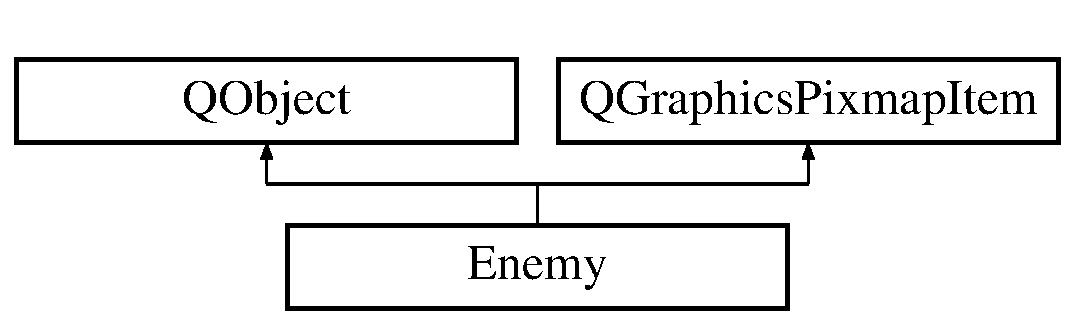
\includegraphics[height=2.000000cm]{class_enemy}
\end{center}
\end{figure}
\subsection*{Public Slots}
\begin{DoxyCompactItemize}
\item 
void \hyperlink{class_enemy_afa4cb14cbeaf872456d223cb8a314928}{move\+\_\+forward} ()
\end{DoxyCompactItemize}
\subsection*{Public Member Functions}
\begin{DoxyCompactItemize}
\item 
\hyperlink{class_enemy_abfd2025e0660f920746f930d59b38bf0}{Enemy} (Q\+List$<$ Q\+PointF $>$ points\+To\+Follow, int enemy\+Number, Q\+Graphics\+Item $\ast$parent=0)
\item 
void \hyperlink{class_enemy_aed33c099d6ec54e1c6cfb676ac38de5b}{rotate\+To\+Point} (Q\+PointF p)
\item 
void \hyperlink{class_enemy_ac7a5e3a071bcc4d67300cfae9446e0bd}{add\+Damage} (int dam)
\item 
int \hyperlink{class_enemy_ab680828a4c84c33a66bea01178cdf3e3}{get\+Loot} () const
\item 
void \hyperlink{class_enemy_ad4139e522aa32c491271155adfb053f0}{set\+Loot} (int value)
\end{DoxyCompactItemize}
\subsection*{Public Attributes}
\begin{DoxyCompactItemize}
\item 
int \hyperlink{class_enemy_aedd5e7bf8ef07ee97be433c853a10d8d}{health}
\item 
int \hyperlink{class_enemy_a8f007e72b954c077e5433a111def78c3}{loot}
\item 
int \hyperlink{class_enemy_aa949fdeff0f2f52bc9e779e69dfc27e0}{S\+T\+E\+P\+\_\+\+S\+I\+ZE}
\item 
Q\+Timer $\ast$ \hyperlink{class_enemy_a70012228edd80bdbf5d71374f0b7ef9e}{timer}
\end{DoxyCompactItemize}
\subsection*{Private Attributes}
\begin{DoxyCompactItemize}
\item 
Q\+List$<$ Q\+PointF $>$ \hyperlink{class_enemy_ae8af9f207c5285b56f7cb190c66994c8}{points}
\item 
Q\+PointF \hyperlink{class_enemy_a50c844f66858b84fc8ebdfccf7e2c535}{dest}
\item 
int \hyperlink{class_enemy_a7291ad5563a976b78fbf6731b353f1c9}{point\+\_\+index}
\item 
Q\+Graphics\+Rect\+Item $\ast$ \hyperlink{class_enemy_ae2613608ff6c6d090a714874e722c340}{healthbar}
\item 
int \hyperlink{class_enemy_a259bfaab0f0d06c9ec2cb15c787e0b3a}{w}
\item 
int \hyperlink{class_enemy_adcb5512e63e735485cbb83f763acce75}{h}
\item 
int \hyperlink{class_enemy_aa5350ac40894832de19d669f0f65af4d}{healthwidth}
\item 
Q\+List$<$ Q\+Pixmap $>$ \hyperlink{class_enemy_ae65aa5ab482bb5eae5c0329c821e5827}{sprites}
\item 
double \hyperlink{class_enemy_a5c11ea6afd7998cf74a6a73dc05d0a63}{scale}
\item 
int \hyperlink{class_enemy_ad36955113c7ac1218b7435d7a87cb846}{sprite\+\_\+counter}
\item 
int \hyperlink{class_enemy_a5e1ff7cda54fcc5ae02925b0ecdbe1bc}{enemy\+Counter}
\end{DoxyCompactItemize}


\subsection{Detailed Description}


Definition at line 12 of file enemy.\+h.



\subsection{Constructor \& Destructor Documentation}
\mbox{\Hypertarget{class_enemy_abfd2025e0660f920746f930d59b38bf0}\label{class_enemy_abfd2025e0660f920746f930d59b38bf0}} 
\index{Enemy@{Enemy}!Enemy@{Enemy}}
\index{Enemy@{Enemy}!Enemy@{Enemy}}
\subsubsection{\texorpdfstring{Enemy()}{Enemy()}}
{\footnotesize\ttfamily Enemy\+::\+Enemy (\begin{DoxyParamCaption}\item[{Q\+List$<$ Q\+PointF $>$}]{points\+To\+Follow,  }\item[{int}]{enemy\+Number,  }\item[{Q\+Graphics\+Item $\ast$}]{parent = {\ttfamily 0} }\end{DoxyParamCaption})}



Definition at line 13 of file enemy.\+cpp.


\begin{DoxyCode}
14 \{
15     \textcolor{comment}{//create enemy sprites}
16     \hyperlink{class_enemy_a5e1ff7cda54fcc5ae02925b0ecdbe1bc}{enemyCounter} = enemyNumber;
17     \textcolor{comment}{//add if parameter for enemy type}
18     QPixmap p(\textcolor{stringliteral}{":/images/images/sprites.png"});
19     QPixmap ouBill(\textcolor{stringliteral}{":/images/images/OuBill.png"});
20     \hyperlink{class_enemy_ae65aa5ab482bb5eae5c0329c821e5827}{sprites}.append(ouBill);
21 
22     \textcolor{keywordflow}{if} (enemyNumber == 1) \{
23         QPixmap eye1 = p.copy(234, 0, 39, 32);
24         \hyperlink{class_enemy_ae65aa5ab482bb5eae5c0329c821e5827}{sprites}.append(eye1);
25         QPixmap eye2 = p.copy(273, 0, 39, 32);
26         \hyperlink{class_enemy_ae65aa5ab482bb5eae5c0329c821e5827}{sprites}.append(eye2);
27         \hyperlink{class_enemy_a5c11ea6afd7998cf74a6a73dc05d0a63}{scale} = 3;
28         \hyperlink{class_enemy_ad36955113c7ac1218b7435d7a87cb846}{sprite\_counter} = enemyNumber;
29     \}
30     \textcolor{keywordflow}{else} \textcolor{keywordflow}{if} (enemyNumber == 0) \{
31         \hyperlink{class_enemy_a5c11ea6afd7998cf74a6a73dc05d0a63}{scale} = 0.8;
32         \hyperlink{class_enemy_ad36955113c7ac1218b7435d7a87cb846}{sprite\_counter} = 0;
33     \} \textcolor{keywordflow}{else} \{
34         \textcolor{keywordflow}{return};
35     \}
36 
37 
38 
39 
40     \textcolor{comment}{//set the graphics}
41     setPixmap(\hyperlink{class_enemy_ae65aa5ab482bb5eae5c0329c821e5827}{sprites}[\hyperlink{class_enemy_ad36955113c7ac1218b7435d7a87cb846}{sprite\_counter}]);
42     setScale(\hyperlink{class_enemy_a5c11ea6afd7998cf74a6a73dc05d0a63}{scale});
43     \hyperlink{class_enemy_a259bfaab0f0d06c9ec2cb15c787e0b3a}{w} = pixmap().width();
44     \hyperlink{class_enemy_adcb5512e63e735485cbb83f763acce75}{h} = pixmap().height();
45     setOffset(-\hyperlink{class_enemy_a259bfaab0f0d06c9ec2cb15c787e0b3a}{w}/2,-\hyperlink{class_enemy_adcb5512e63e735485cbb83f763acce75}{h}/2);
46 
47     \textcolor{comment}{//set points}
48     \hyperlink{class_enemy_ae8af9f207c5285b56f7cb190c66994c8}{points} << pointsToFollow;
49     \hyperlink{class_enemy_a7291ad5563a976b78fbf6731b353f1c9}{point\_index} = 0;
50     \hyperlink{class_enemy_a50c844f66858b84fc8ebdfccf7e2c535}{dest} = \hyperlink{class_enemy_ae8af9f207c5285b56f7cb190c66994c8}{points}[0];
51     \hyperlink{class_enemy_aed33c099d6ec54e1c6cfb676ac38de5b}{rotateToPoint}(\hyperlink{class_enemy_a50c844f66858b84fc8ebdfccf7e2c535}{dest});
52 
53     \textcolor{comment}{//connect time to move}
54     connect(\hyperlink{enemy_8cpp_a58bdb5643d0814ac4e697a1564b79b70}{game}->\hyperlink{class_game_a8feee9081542b15a9f2d889a6f1c8257}{gametimer}, SIGNAL(timeout()), \textcolor{keyword}{this}, SLOT(
      \hyperlink{class_enemy_afa4cb14cbeaf872456d223cb8a314928}{move\_forward}()));
55 
56     \textcolor{comment}{//enemy default stats}
57     \hyperlink{class_enemy_aedd5e7bf8ef07ee97be433c853a10d8d}{health} = 2500;
58     \hyperlink{class_enemy_a8f007e72b954c077e5433a111def78c3}{loot} = 50;
59 
60     \textcolor{comment}{//make health bar}
61     \hyperlink{class_enemy_aa5350ac40894832de19d669f0f65af4d}{healthwidth} = \hyperlink{class_enemy_aedd5e7bf8ef07ee97be433c853a10d8d}{health}/50+\hyperlink{enemy_8cpp_a58bdb5643d0814ac4e697a1564b79b70}{game}->\hyperlink{class_game_af9a4b49ad573785e961b29758c84fdd0}{wave}->\hyperlink{class_waves_abfdc18a5f2f185285173797c1c67c6f9}{waveLevel};
62     \hyperlink{class_enemy_ae2613608ff6c6d090a714874e722c340}{healthbar} = \textcolor{keyword}{new} QGraphicsRectItem(\textcolor{keyword}{this});
63     \hyperlink{class_enemy_ae2613608ff6c6d090a714874e722c340}{healthbar}->setRect(-\hyperlink{class_enemy_a259bfaab0f0d06c9ec2cb15c787e0b3a}{w}/4,-\hyperlink{class_enemy_adcb5512e63e735485cbb83f763acce75}{h}/1.8, \hyperlink{class_enemy_aa5350ac40894832de19d669f0f65af4d}{healthwidth}/\hyperlink{class_enemy_a5c11ea6afd7998cf74a6a73dc05d0a63}{scale},10/
      \hyperlink{class_enemy_a5c11ea6afd7998cf74a6a73dc05d0a63}{scale});
64     QBrush brush;
65     brush.setStyle(Qt::SolidPattern);
66     brush.setColor(QColor(255,50,20));
67     \hyperlink{class_enemy_ae2613608ff6c6d090a714874e722c340}{healthbar}->setBrush(brush);
68 
69 
70 \}
\end{DoxyCode}


\subsection{Member Function Documentation}
\mbox{\Hypertarget{class_enemy_ac7a5e3a071bcc4d67300cfae9446e0bd}\label{class_enemy_ac7a5e3a071bcc4d67300cfae9446e0bd}} 
\index{Enemy@{Enemy}!add\+Damage@{add\+Damage}}
\index{add\+Damage@{add\+Damage}!Enemy@{Enemy}}
\subsubsection{\texorpdfstring{add\+Damage()}{addDamage()}}
{\footnotesize\ttfamily void Enemy\+::add\+Damage (\begin{DoxyParamCaption}\item[{int}]{dam }\end{DoxyParamCaption})}



Definition at line 88 of file enemy.\+cpp.


\begin{DoxyCode}
89 \{
90     \hyperlink{class_enemy_aedd5e7bf8ef07ee97be433c853a10d8d}{health} += -dam;
91     \textcolor{comment}{//healthwidth = health/50+game->wave->waveLevel;}
92     \hyperlink{class_enemy_ae2613608ff6c6d090a714874e722c340}{healthbar}->setRect(-\hyperlink{class_enemy_a259bfaab0f0d06c9ec2cb15c787e0b3a}{w}/4, -\hyperlink{class_enemy_adcb5512e63e735485cbb83f763acce75}{h}/1.8, (\hyperlink{class_enemy_aedd5e7bf8ef07ee97be433c853a10d8d}{health}-dam)/\hyperlink{class_enemy_aa5350ac40894832de19d669f0f65af4d}{healthwidth}/
      \hyperlink{class_enemy_a5c11ea6afd7998cf74a6a73dc05d0a63}{scale}, 10/\hyperlink{class_enemy_a5c11ea6afd7998cf74a6a73dc05d0a63}{scale});
93 
94 \}
\end{DoxyCode}
\mbox{\Hypertarget{class_enemy_ab680828a4c84c33a66bea01178cdf3e3}\label{class_enemy_ab680828a4c84c33a66bea01178cdf3e3}} 
\index{Enemy@{Enemy}!get\+Loot@{get\+Loot}}
\index{get\+Loot@{get\+Loot}!Enemy@{Enemy}}
\subsubsection{\texorpdfstring{get\+Loot()}{getLoot()}}
{\footnotesize\ttfamily int Enemy\+::get\+Loot (\begin{DoxyParamCaption}{ }\end{DoxyParamCaption}) const}



Definition at line 78 of file enemy.\+cpp.


\begin{DoxyCode}
79 \{
80     \textcolor{keywordflow}{return} \hyperlink{class_enemy_a8f007e72b954c077e5433a111def78c3}{loot};
81 \}
\end{DoxyCode}
\mbox{\Hypertarget{class_enemy_afa4cb14cbeaf872456d223cb8a314928}\label{class_enemy_afa4cb14cbeaf872456d223cb8a314928}} 
\index{Enemy@{Enemy}!move\+\_\+forward@{move\+\_\+forward}}
\index{move\+\_\+forward@{move\+\_\+forward}!Enemy@{Enemy}}
\subsubsection{\texorpdfstring{move\+\_\+forward}{move\_forward}}
{\footnotesize\ttfamily void Enemy\+::move\+\_\+forward (\begin{DoxyParamCaption}{ }\end{DoxyParamCaption})\hspace{0.3cm}{\ttfamily [slot]}}



Definition at line 96 of file enemy.\+cpp.


\begin{DoxyCode}
97 \{
98     \textcolor{comment}{//swap pixmap}
99     \textcolor{keywordflow}{switch} (\hyperlink{class_enemy_ad36955113c7ac1218b7435d7a87cb846}{sprite\_counter}) \{
100     \textcolor{keywordflow}{case} 0:
101         setPixmap(\hyperlink{class_enemy_ae65aa5ab482bb5eae5c0329c821e5827}{sprites}[0]);
102         \textcolor{keywordflow}{break};
103     \textcolor{keywordflow}{case} 1:
104         setPixmap(\hyperlink{class_enemy_ae65aa5ab482bb5eae5c0329c821e5827}{sprites}[1]);
105         \hyperlink{class_enemy_ad36955113c7ac1218b7435d7a87cb846}{sprite\_counter}++;
106         \textcolor{keywordflow}{break};
107     \textcolor{keywordflow}{case} 2:
108         setPixmap(\hyperlink{class_enemy_ae65aa5ab482bb5eae5c0329c821e5827}{sprites}[2]);
109         \hyperlink{class_enemy_ad36955113c7ac1218b7435d7a87cb846}{sprite\_counter}--;
110         \textcolor{keywordflow}{break};
111     \textcolor{keywordflow}{default}:
112         \textcolor{keywordflow}{break};
113     \}
114 
115 
116 
117     \textcolor{comment}{//if close to dest, rotate to next dest}
118     QLineF ln(pos(),\hyperlink{class_enemy_a50c844f66858b84fc8ebdfccf7e2c535}{dest});
119     \textcolor{keywordflow}{if} ((ln.length() <5))
120     \{
121         \hyperlink{class_enemy_a7291ad5563a976b78fbf6731b353f1c9}{point\_index}++;
122         \textcolor{keywordflow}{if} (\hyperlink{class_enemy_a7291ad5563a976b78fbf6731b353f1c9}{point\_index} >= \hyperlink{class_enemy_ae8af9f207c5285b56f7cb190c66994c8}{points}.size())\{
123             \textcolor{keywordflow}{return};
124         \}
125         \hyperlink{class_enemy_a50c844f66858b84fc8ebdfccf7e2c535}{dest} = \hyperlink{class_enemy_ae8af9f207c5285b56f7cb190c66994c8}{points}[\hyperlink{class_enemy_a7291ad5563a976b78fbf6731b353f1c9}{point\_index}];
126         \hyperlink{class_enemy_aed33c099d6ec54e1c6cfb676ac38de5b}{rotateToPoint}(\hyperlink{class_enemy_a50c844f66858b84fc8ebdfccf7e2c535}{dest});
127     \}
128 
129     \textcolor{comment}{//move enemy at current angle}
130     \hyperlink{class_enemy_aa949fdeff0f2f52bc9e779e69dfc27e0}{STEP\_SIZE} = 5;
131     \textcolor{keywordtype}{double} theta = rotation(); \textcolor{comment}{//degrees}
132 
133     \textcolor{keywordtype}{double} dy = \hyperlink{class_enemy_aa949fdeff0f2f52bc9e779e69dfc27e0}{STEP\_SIZE} * qSin(qDegreesToRadians(theta));
134     \textcolor{keywordtype}{double} dx = \hyperlink{class_enemy_aa949fdeff0f2f52bc9e779e69dfc27e0}{STEP\_SIZE} * qCos(qDegreesToRadians(theta));
135 
136     setPos(x()+dx, y()+dy);
137 
138     \hyperlink{enemy_8cpp_a58bdb5643d0814ac4e697a1564b79b70}{game}->\hyperlink{class_game_ae0adfbcc271a45a2c3ede2c6b948beda}{closestNode}(x(),y());
139     \textcolor{keywordtype}{int} y\_map = (\hyperlink{enemy_8cpp_a58bdb5643d0814ac4e697a1564b79b70}{game}->\hyperlink{class_game_a861bf240380d110b285659d8af3f0406}{closestNodePos}.y() -\hyperlink{enemy_8cpp_a7bdaf8655b48f0d7994eb54ec1da4981}{map}->\hyperlink{class_map_a483dfba507cee9d2fa60a074992b1fcf}{tileY}/2)/
      \hyperlink{enemy_8cpp_a7bdaf8655b48f0d7994eb54ec1da4981}{map}->\hyperlink{class_map_a483dfba507cee9d2fa60a074992b1fcf}{tileY};
140     setZValue(y\_map);
141 
142     \textcolor{comment}{//if position at end node deconstruct enemy and take life}
143     \textcolor{keywordflow}{if} (y()>= \hyperlink{enemy_8cpp_a7bdaf8655b48f0d7994eb54ec1da4981}{map}->\hyperlink{class_map_ae08efae9ac1453b2690985c627aca358}{mapY}*\hyperlink{enemy_8cpp_a7bdaf8655b48f0d7994eb54ec1da4981}{map}->\hyperlink{class_map_a483dfba507cee9d2fa60a074992b1fcf}{tileY} - \hyperlink{enemy_8cpp_a7bdaf8655b48f0d7994eb54ec1da4981}{map}->\hyperlink{class_map_a483dfba507cee9d2fa60a074992b1fcf}{tileY}) \{
144         \textcolor{comment}{//remove a live}
145         \hyperlink{enemy_8cpp_a58bdb5643d0814ac4e697a1564b79b70}{game}->\hyperlink{class_game_ad8a7cc146f99c7ec5b7c3c25d73f118c}{player1}->\hyperlink{class_player1_aacba034528d5c9fdefa4f246fe526a38}{Lives} += -1;
146         \hyperlink{enemy_8cpp_a58bdb5643d0814ac4e697a1564b79b70}{game}->\hyperlink{class_game_aa5e4edca458d1a1378d035a138d69635}{updateLives}();
147 
148         \textcolor{comment}{//play quack}
149         QSound *quack = \textcolor{keyword}{new} QSound(\textcolor{stringliteral}{":/images/sounds/quack.wav"});
150         quack->play();
151 
152         \textcolor{comment}{//if all lives are gone}
153         \textcolor{keywordflow}{if} (\hyperlink{enemy_8cpp_a58bdb5643d0814ac4e697a1564b79b70}{game}->\hyperlink{class_game_ad8a7cc146f99c7ec5b7c3c25d73f118c}{player1}->\hyperlink{class_player1_aacba034528d5c9fdefa4f246fe526a38}{Lives} <= 0) \{
154             \hyperlink{enemy_8cpp_a58bdb5643d0814ac4e697a1564b79b70}{game}->\hyperlink{class_game_a838e89640d4cfbd7d7b7ee105135d4b8}{GAMEOVER}();
155             \textcolor{keywordflow}{return};
156         \}
157 
158         deleteLater();
159         \hyperlink{enemy_8cpp_a58bdb5643d0814ac4e697a1564b79b70}{game}->\hyperlink{class_game_ab96914bfc1e59035233105abfb0787fe}{listOfEnemies}.removeOne(\textcolor{keyword}{this});
160         \textcolor{comment}{//delete this;}
161         \textcolor{keywordflow}{return};
162     \}
163 \}
\end{DoxyCode}
\mbox{\Hypertarget{class_enemy_aed33c099d6ec54e1c6cfb676ac38de5b}\label{class_enemy_aed33c099d6ec54e1c6cfb676ac38de5b}} 
\index{Enemy@{Enemy}!rotate\+To\+Point@{rotate\+To\+Point}}
\index{rotate\+To\+Point@{rotate\+To\+Point}!Enemy@{Enemy}}
\subsubsection{\texorpdfstring{rotate\+To\+Point()}{rotateToPoint()}}
{\footnotesize\ttfamily void Enemy\+::rotate\+To\+Point (\begin{DoxyParamCaption}\item[{Q\+PointF}]{p }\end{DoxyParamCaption})}



Definition at line 72 of file enemy.\+cpp.


\begin{DoxyCode}
73 \{
74     QLineF ln(pos(),p);
75     setRotation(-1 * ln.angle());
76 \}
\end{DoxyCode}
\mbox{\Hypertarget{class_enemy_ad4139e522aa32c491271155adfb053f0}\label{class_enemy_ad4139e522aa32c491271155adfb053f0}} 
\index{Enemy@{Enemy}!set\+Loot@{set\+Loot}}
\index{set\+Loot@{set\+Loot}!Enemy@{Enemy}}
\subsubsection{\texorpdfstring{set\+Loot()}{setLoot()}}
{\footnotesize\ttfamily void Enemy\+::set\+Loot (\begin{DoxyParamCaption}\item[{int}]{value }\end{DoxyParamCaption})}



Definition at line 83 of file enemy.\+cpp.


\begin{DoxyCode}
84 \{
85     \hyperlink{class_enemy_a8f007e72b954c077e5433a111def78c3}{loot} = value;
86 \}
\end{DoxyCode}


\subsection{Member Data Documentation}
\mbox{\Hypertarget{class_enemy_a50c844f66858b84fc8ebdfccf7e2c535}\label{class_enemy_a50c844f66858b84fc8ebdfccf7e2c535}} 
\index{Enemy@{Enemy}!dest@{dest}}
\index{dest@{dest}!Enemy@{Enemy}}
\subsubsection{\texorpdfstring{dest}{dest}}
{\footnotesize\ttfamily Q\+PointF Enemy\+::dest\hspace{0.3cm}{\ttfamily [private]}}



Definition at line 32 of file enemy.\+h.

\mbox{\Hypertarget{class_enemy_a5e1ff7cda54fcc5ae02925b0ecdbe1bc}\label{class_enemy_a5e1ff7cda54fcc5ae02925b0ecdbe1bc}} 
\index{Enemy@{Enemy}!enemy\+Counter@{enemy\+Counter}}
\index{enemy\+Counter@{enemy\+Counter}!Enemy@{Enemy}}
\subsubsection{\texorpdfstring{enemy\+Counter}{enemyCounter}}
{\footnotesize\ttfamily int Enemy\+::enemy\+Counter\hspace{0.3cm}{\ttfamily [private]}}



Definition at line 41 of file enemy.\+h.

\mbox{\Hypertarget{class_enemy_adcb5512e63e735485cbb83f763acce75}\label{class_enemy_adcb5512e63e735485cbb83f763acce75}} 
\index{Enemy@{Enemy}!h@{h}}
\index{h@{h}!Enemy@{Enemy}}
\subsubsection{\texorpdfstring{h}{h}}
{\footnotesize\ttfamily int Enemy\+::h\hspace{0.3cm}{\ttfamily [private]}}



Definition at line 36 of file enemy.\+h.

\mbox{\Hypertarget{class_enemy_aedd5e7bf8ef07ee97be433c853a10d8d}\label{class_enemy_aedd5e7bf8ef07ee97be433c853a10d8d}} 
\index{Enemy@{Enemy}!health@{health}}
\index{health@{health}!Enemy@{Enemy}}
\subsubsection{\texorpdfstring{health}{health}}
{\footnotesize\ttfamily int Enemy\+::health}



Definition at line 18 of file enemy.\+h.

\mbox{\Hypertarget{class_enemy_ae2613608ff6c6d090a714874e722c340}\label{class_enemy_ae2613608ff6c6d090a714874e722c340}} 
\index{Enemy@{Enemy}!healthbar@{healthbar}}
\index{healthbar@{healthbar}!Enemy@{Enemy}}
\subsubsection{\texorpdfstring{healthbar}{healthbar}}
{\footnotesize\ttfamily Q\+Graphics\+Rect\+Item$\ast$ Enemy\+::healthbar\hspace{0.3cm}{\ttfamily [private]}}



Definition at line 34 of file enemy.\+h.

\mbox{\Hypertarget{class_enemy_aa5350ac40894832de19d669f0f65af4d}\label{class_enemy_aa5350ac40894832de19d669f0f65af4d}} 
\index{Enemy@{Enemy}!healthwidth@{healthwidth}}
\index{healthwidth@{healthwidth}!Enemy@{Enemy}}
\subsubsection{\texorpdfstring{healthwidth}{healthwidth}}
{\footnotesize\ttfamily int Enemy\+::healthwidth\hspace{0.3cm}{\ttfamily [private]}}



Definition at line 37 of file enemy.\+h.

\mbox{\Hypertarget{class_enemy_a8f007e72b954c077e5433a111def78c3}\label{class_enemy_a8f007e72b954c077e5433a111def78c3}} 
\index{Enemy@{Enemy}!loot@{loot}}
\index{loot@{loot}!Enemy@{Enemy}}
\subsubsection{\texorpdfstring{loot}{loot}}
{\footnotesize\ttfamily int Enemy\+::loot}



Definition at line 19 of file enemy.\+h.

\mbox{\Hypertarget{class_enemy_a7291ad5563a976b78fbf6731b353f1c9}\label{class_enemy_a7291ad5563a976b78fbf6731b353f1c9}} 
\index{Enemy@{Enemy}!point\+\_\+index@{point\+\_\+index}}
\index{point\+\_\+index@{point\+\_\+index}!Enemy@{Enemy}}
\subsubsection{\texorpdfstring{point\+\_\+index}{point\_index}}
{\footnotesize\ttfamily int Enemy\+::point\+\_\+index\hspace{0.3cm}{\ttfamily [private]}}



Definition at line 33 of file enemy.\+h.

\mbox{\Hypertarget{class_enemy_ae8af9f207c5285b56f7cb190c66994c8}\label{class_enemy_ae8af9f207c5285b56f7cb190c66994c8}} 
\index{Enemy@{Enemy}!points@{points}}
\index{points@{points}!Enemy@{Enemy}}
\subsubsection{\texorpdfstring{points}{points}}
{\footnotesize\ttfamily Q\+List$<$Q\+PointF$>$ Enemy\+::points\hspace{0.3cm}{\ttfamily [private]}}



Definition at line 31 of file enemy.\+h.

\mbox{\Hypertarget{class_enemy_a5c11ea6afd7998cf74a6a73dc05d0a63}\label{class_enemy_a5c11ea6afd7998cf74a6a73dc05d0a63}} 
\index{Enemy@{Enemy}!scale@{scale}}
\index{scale@{scale}!Enemy@{Enemy}}
\subsubsection{\texorpdfstring{scale}{scale}}
{\footnotesize\ttfamily double Enemy\+::scale\hspace{0.3cm}{\ttfamily [private]}}



Definition at line 39 of file enemy.\+h.

\mbox{\Hypertarget{class_enemy_ad36955113c7ac1218b7435d7a87cb846}\label{class_enemy_ad36955113c7ac1218b7435d7a87cb846}} 
\index{Enemy@{Enemy}!sprite\+\_\+counter@{sprite\+\_\+counter}}
\index{sprite\+\_\+counter@{sprite\+\_\+counter}!Enemy@{Enemy}}
\subsubsection{\texorpdfstring{sprite\+\_\+counter}{sprite\_counter}}
{\footnotesize\ttfamily int Enemy\+::sprite\+\_\+counter\hspace{0.3cm}{\ttfamily [private]}}



Definition at line 40 of file enemy.\+h.

\mbox{\Hypertarget{class_enemy_ae65aa5ab482bb5eae5c0329c821e5827}\label{class_enemy_ae65aa5ab482bb5eae5c0329c821e5827}} 
\index{Enemy@{Enemy}!sprites@{sprites}}
\index{sprites@{sprites}!Enemy@{Enemy}}
\subsubsection{\texorpdfstring{sprites}{sprites}}
{\footnotesize\ttfamily Q\+List$<$Q\+Pixmap$>$ Enemy\+::sprites\hspace{0.3cm}{\ttfamily [private]}}



Definition at line 38 of file enemy.\+h.

\mbox{\Hypertarget{class_enemy_aa949fdeff0f2f52bc9e779e69dfc27e0}\label{class_enemy_aa949fdeff0f2f52bc9e779e69dfc27e0}} 
\index{Enemy@{Enemy}!S\+T\+E\+P\+\_\+\+S\+I\+ZE@{S\+T\+E\+P\+\_\+\+S\+I\+ZE}}
\index{S\+T\+E\+P\+\_\+\+S\+I\+ZE@{S\+T\+E\+P\+\_\+\+S\+I\+ZE}!Enemy@{Enemy}}
\subsubsection{\texorpdfstring{S\+T\+E\+P\+\_\+\+S\+I\+ZE}{STEP\_SIZE}}
{\footnotesize\ttfamily int Enemy\+::\+S\+T\+E\+P\+\_\+\+S\+I\+ZE}



Definition at line 21 of file enemy.\+h.

\mbox{\Hypertarget{class_enemy_a70012228edd80bdbf5d71374f0b7ef9e}\label{class_enemy_a70012228edd80bdbf5d71374f0b7ef9e}} 
\index{Enemy@{Enemy}!timer@{timer}}
\index{timer@{timer}!Enemy@{Enemy}}
\subsubsection{\texorpdfstring{timer}{timer}}
{\footnotesize\ttfamily Q\+Timer$\ast$ Enemy\+::timer}



Definition at line 22 of file enemy.\+h.

\mbox{\Hypertarget{class_enemy_a259bfaab0f0d06c9ec2cb15c787e0b3a}\label{class_enemy_a259bfaab0f0d06c9ec2cb15c787e0b3a}} 
\index{Enemy@{Enemy}!w@{w}}
\index{w@{w}!Enemy@{Enemy}}
\subsubsection{\texorpdfstring{w}{w}}
{\footnotesize\ttfamily int Enemy\+::w\hspace{0.3cm}{\ttfamily [private]}}



Definition at line 35 of file enemy.\+h.



The documentation for this class was generated from the following files\+:\begin{DoxyCompactItemize}
\item 
C\+:/\+Users/\+Fu\+Zzy/\+Dropbox/3de Jaar/\+Sem 1/\+R\+E\+I\+I313-\/\+C++ O\+O\+P/\+T\+D\+\_\+\+Game/\+Element\+\_\+\+T\+D/\hyperlink{enemy_8h}{enemy.\+h}\item 
C\+:/\+Users/\+Fu\+Zzy/\+Dropbox/3de Jaar/\+Sem 1/\+R\+E\+I\+I313-\/\+C++ O\+O\+P/\+T\+D\+\_\+\+Game/\+Element\+\_\+\+T\+D/\hyperlink{enemy_8cpp}{enemy.\+cpp}\end{DoxyCompactItemize}

\hypertarget{class_fire_tower}{}\section{Fire\+Tower Class Reference}
\label{class_fire_tower}\index{Fire\+Tower@{Fire\+Tower}}


{\ttfamily \#include $<$firetower.\+h$>$}

Inheritance diagram for Fire\+Tower\+:\begin{figure}[H]
\begin{center}
\leavevmode
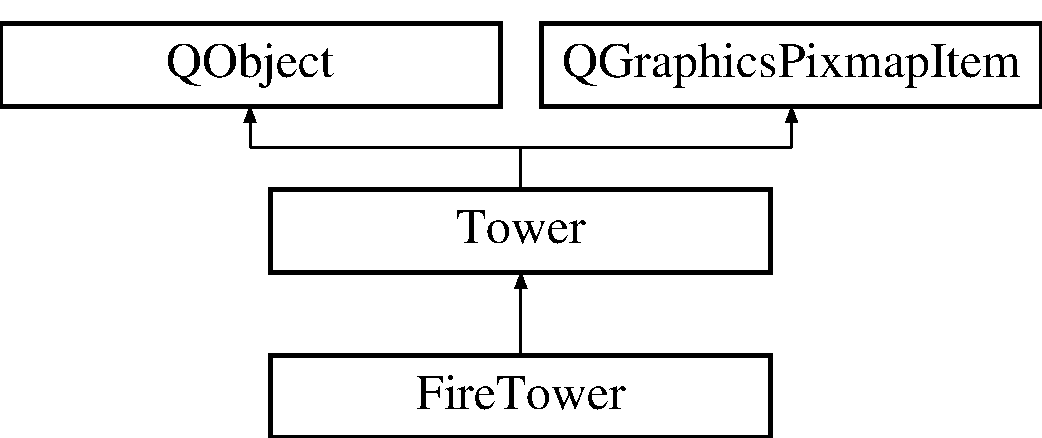
\includegraphics[height=3.000000cm]{class_fire_tower}
\end{center}
\end{figure}
\subsection*{Public Slots}
\begin{DoxyCompactItemize}
\item 
void \hyperlink{class_fire_tower_a4a3c1e246ed66479aabff4ab5d187636}{aquire\+\_\+target} ()
\end{DoxyCompactItemize}
\subsection*{Public Member Functions}
\begin{DoxyCompactItemize}
\item 
\hyperlink{class_fire_tower_ad375e5ef0c469832741f6a541f3caae1}{Fire\+Tower} (Q\+Graphics\+Item $\ast$parent=0)
\item 
void \hyperlink{class_fire_tower_a9a0b13fcb0bc204194d953c5494afbe3}{fire} ()
\item 
int \hyperlink{class_fire_tower_a74be102e9bb0871f19fb55b434e2b6d7}{get\+Cost\+Of\+Tower} ()
\item 
void \hyperlink{class_fire_tower_a1768ca309eccef5f7f093f37741ba572}{mouse\+Press\+Event} (Q\+Graphics\+Scene\+Mouse\+Event $\ast$event)
\item 
void \hyperlink{class_fire_tower_a4deed164ccfbabcd7fc67e3973015f9f}{mouse\+Double\+Click\+Event} (Q\+Graphics\+Scene\+Mouse\+Event $\ast$event)
\item 
void \hyperlink{class_fire_tower_adc1bcb15312eac1dd9788be48e55baad}{sell\+Tower} ()
\end{DoxyCompactItemize}
\subsection*{Public Attributes}
\begin{DoxyCompactItemize}
\item 
const int \hyperlink{class_fire_tower_ae05eab1ea0a68b5109ee91771d3c8569}{cost\+Of\+Tower} = 300
\end{DoxyCompactItemize}
\subsection*{Private Attributes}
\begin{DoxyCompactItemize}
\item 
int \hyperlink{class_fire_tower_a59a01cc273823ea5451179dbc1f4aded}{tower\+Damage}
\end{DoxyCompactItemize}
\subsection*{Additional Inherited Members}


\subsection{Detailed Description}


Definition at line 7 of file firetower.\+h.



\subsection{Constructor \& Destructor Documentation}
\mbox{\Hypertarget{class_fire_tower_ad375e5ef0c469832741f6a541f3caae1}\label{class_fire_tower_ad375e5ef0c469832741f6a541f3caae1}} 
\index{Fire\+Tower@{Fire\+Tower}!Fire\+Tower@{Fire\+Tower}}
\index{Fire\+Tower@{Fire\+Tower}!Fire\+Tower@{Fire\+Tower}}
\subsubsection{\texorpdfstring{Fire\+Tower()}{FireTower()}}
{\footnotesize\ttfamily Fire\+Tower\+::\+Fire\+Tower (\begin{DoxyParamCaption}\item[{Q\+Graphics\+Item $\ast$}]{parent = {\ttfamily 0} }\end{DoxyParamCaption})}



Definition at line 9 of file firetower.\+cpp.


\begin{DoxyCode}
10 \{
11     \textcolor{comment}{//set graphics}
12     setPixmap(QPixmap(\textcolor{stringliteral}{":/images/images/Tower\_Fire.png"}));
13     \textcolor{keywordtype}{int} w = pixmap().width();
14     \textcolor{keywordtype}{int} h = pixmap().height();
15     setOffset(-w/2,-h/1.25);
16 
17 
18     \textcolor{comment}{//connect timer to aaquire target}
19     QTimer * timer = \textcolor{keyword}{new} QTimer();
20     connect(timer,SIGNAL(timeout()),\textcolor{keyword}{this},SLOT(\hyperlink{class_fire_tower_a4a3c1e246ed66479aabff4ab5d187636}{aquire\_target}()));
21     timer->start(1000);
22 
23 \}
\end{DoxyCode}


\subsection{Member Function Documentation}
\mbox{\Hypertarget{class_fire_tower_a4a3c1e246ed66479aabff4ab5d187636}\label{class_fire_tower_a4a3c1e246ed66479aabff4ab5d187636}} 
\index{Fire\+Tower@{Fire\+Tower}!aquire\+\_\+target@{aquire\+\_\+target}}
\index{aquire\+\_\+target@{aquire\+\_\+target}!Fire\+Tower@{Fire\+Tower}}
\subsubsection{\texorpdfstring{aquire\+\_\+target}{aquire\_target}}
{\footnotesize\ttfamily void Fire\+Tower\+::aquire\+\_\+target (\begin{DoxyParamCaption}{ }\end{DoxyParamCaption})\hspace{0.3cm}{\ttfamily [slot]}}



Definition at line 55 of file firetower.\+cpp.


\begin{DoxyCode}
56 \{
57     \hyperlink{class_tower_a6e0df1e43e746622967918aaf6f42dce}{Tower::aquire\_target}();
58 \}
\end{DoxyCode}
\mbox{\Hypertarget{class_fire_tower_a9a0b13fcb0bc204194d953c5494afbe3}\label{class_fire_tower_a9a0b13fcb0bc204194d953c5494afbe3}} 
\index{Fire\+Tower@{Fire\+Tower}!fire@{fire}}
\index{fire@{fire}!Fire\+Tower@{Fire\+Tower}}
\subsubsection{\texorpdfstring{fire()}{fire()}}
{\footnotesize\ttfamily void Fire\+Tower\+::fire (\begin{DoxyParamCaption}{ }\end{DoxyParamCaption})\hspace{0.3cm}{\ttfamily [virtual]}}



Reimplemented from \hyperlink{class_tower_aa0c9c780f48cffacd3da6877f5d4fdc2}{Tower}.



Definition at line 25 of file firetower.\+cpp.


\begin{DoxyCode}
26 \{
27     \textcolor{comment}{//create the bullets}
28     \hyperlink{class_bullet}{Bullet} *bullet = \textcolor{keyword}{new} \hyperlink{class_bullet}{Bullet}();
29 
30     \textcolor{comment}{//set the graphics}
31     bullet->setPixmap(QPixmap(\textcolor{stringliteral}{":/images/images/Projectile\_Fire-min.png"}));
32     \textcolor{comment}{//bullet->setScale(game->scalingfactor\_bullets);}
33 
34     \textcolor{comment}{//set the damage}
35     bullet->\hyperlink{class_bullet_a733d2ebbf9143c9ca68d3eb7e14121d0}{damage} = 40;
36 
37     \textcolor{keywordtype}{int} y\_pos = pixmap().height()*\hyperlink{firetower_8cpp_a58bdb5643d0814ac4e697a1564b79b70}{game}->\hyperlink{class_game_a6c1ca48f17f6934432d01bfa7f762a04}{scalingfactor\_towers}/1.25; \textcolor{comment}{//make it shoot
       from top of tower}
38 
39     bullet->setPos(x(), y()-y\_pos);
40 
41     QLineF ln(QPointF(x(), y()-y\_pos),\hyperlink{class_tower_a2b3e8ab90ccceed1fa3a667db80c2c06}{attack\_dest});
42     \textcolor{keywordtype}{int} angle = -1*ln.angle();
43 
44     bullet->setRotation(angle);
45 
46     \hyperlink{firetower_8cpp_a58bdb5643d0814ac4e697a1564b79b70}{game}->\hyperlink{class_game_a8119e3b9a632906c6808fa294b46a92a}{scene}->addItem(bullet);
47 
48 \}
\end{DoxyCode}
\mbox{\Hypertarget{class_fire_tower_a74be102e9bb0871f19fb55b434e2b6d7}\label{class_fire_tower_a74be102e9bb0871f19fb55b434e2b6d7}} 
\index{Fire\+Tower@{Fire\+Tower}!get\+Cost\+Of\+Tower@{get\+Cost\+Of\+Tower}}
\index{get\+Cost\+Of\+Tower@{get\+Cost\+Of\+Tower}!Fire\+Tower@{Fire\+Tower}}
\subsubsection{\texorpdfstring{get\+Cost\+Of\+Tower()}{getCostOfTower()}}
{\footnotesize\ttfamily int Fire\+Tower\+::get\+Cost\+Of\+Tower (\begin{DoxyParamCaption}{ }\end{DoxyParamCaption})\hspace{0.3cm}{\ttfamily [virtual]}}



Reimplemented from \hyperlink{class_tower_ae1d3f44d0149c8146ccf6b262a52ddad}{Tower}.



Definition at line 50 of file firetower.\+cpp.


\begin{DoxyCode}
51 \{
52     \textcolor{keywordflow}{return} \hyperlink{class_fire_tower_ae05eab1ea0a68b5109ee91771d3c8569}{costOfTower};
53 \}
\end{DoxyCode}
\mbox{\Hypertarget{class_fire_tower_a4deed164ccfbabcd7fc67e3973015f9f}\label{class_fire_tower_a4deed164ccfbabcd7fc67e3973015f9f}} 
\index{Fire\+Tower@{Fire\+Tower}!mouse\+Double\+Click\+Event@{mouse\+Double\+Click\+Event}}
\index{mouse\+Double\+Click\+Event@{mouse\+Double\+Click\+Event}!Fire\+Tower@{Fire\+Tower}}
\subsubsection{\texorpdfstring{mouse\+Double\+Click\+Event()}{mouseDoubleClickEvent()}}
{\footnotesize\ttfamily void Fire\+Tower\+::mouse\+Double\+Click\+Event (\begin{DoxyParamCaption}\item[{Q\+Graphics\+Scene\+Mouse\+Event $\ast$}]{event }\end{DoxyParamCaption})}



Definition at line 78 of file firetower.\+cpp.


\begin{DoxyCode}
79 \{
80     \textcolor{comment}{//upgrade tower}
81     setPixmap(QPixmap(\textcolor{stringliteral}{":/images/images/Tower\_Fire\_2.png"}));
82     \textcolor{keywordtype}{int} w = pixmap().width();
83     \textcolor{keywordtype}{int} h = pixmap().height();
84     setOffset(-w/2,-h/1.25);
85 
86     \textcolor{comment}{//upgrade damage}
87     \hyperlink{class_fire_tower_a59a01cc273823ea5451179dbc1f4aded}{towerDamage} = 70;
88 
89     \textcolor{comment}{//update gold}
90     \hyperlink{firetower_8cpp_a58bdb5643d0814ac4e697a1564b79b70}{game}->\hyperlink{class_game_ad8a7cc146f99c7ec5b7c3c25d73f118c}{player1}->\hyperlink{class_player1_ab390478b345e443398bac442a04b675c}{Gold} += -\hyperlink{class_fire_tower_ae05eab1ea0a68b5109ee91771d3c8569}{costOfTower}/2;
91     \hyperlink{firetower_8cpp_a58bdb5643d0814ac4e697a1564b79b70}{game}->\hyperlink{class_game_a065998f7609f63e2987ede928359595a}{updateGold}();
92 
93 \}
\end{DoxyCode}
\mbox{\Hypertarget{class_fire_tower_a1768ca309eccef5f7f093f37741ba572}\label{class_fire_tower_a1768ca309eccef5f7f093f37741ba572}} 
\index{Fire\+Tower@{Fire\+Tower}!mouse\+Press\+Event@{mouse\+Press\+Event}}
\index{mouse\+Press\+Event@{mouse\+Press\+Event}!Fire\+Tower@{Fire\+Tower}}
\subsubsection{\texorpdfstring{mouse\+Press\+Event()}{mousePressEvent()}}
{\footnotesize\ttfamily void Fire\+Tower\+::mouse\+Press\+Event (\begin{DoxyParamCaption}\item[{Q\+Graphics\+Scene\+Mouse\+Event $\ast$}]{event }\end{DoxyParamCaption})}



Definition at line 61 of file firetower.\+cpp.


\begin{DoxyCode}
62 \{
63 
64    qDebug() << \textcolor{stringliteral}{"Clicked Tower"};
65 
66    \textcolor{comment}{//right mouse sell}
67     \textcolor{keywordflow}{if} (event->button() == Qt::RightButton) \{
68         \hyperlink{class_fire_tower_adc1bcb15312eac1dd9788be48e55baad}{sellTower}();
69     \}
70     \textcolor{keywordflow}{else}
71     \{
72         \textcolor{comment}{//        QGraphicsView::mousePressEvent(event);}
73         \textcolor{keywordflow}{return};
74     \}
75 
76 \}
\end{DoxyCode}
\mbox{\Hypertarget{class_fire_tower_adc1bcb15312eac1dd9788be48e55baad}\label{class_fire_tower_adc1bcb15312eac1dd9788be48e55baad}} 
\index{Fire\+Tower@{Fire\+Tower}!sell\+Tower@{sell\+Tower}}
\index{sell\+Tower@{sell\+Tower}!Fire\+Tower@{Fire\+Tower}}
\subsubsection{\texorpdfstring{sell\+Tower()}{sellTower()}}
{\footnotesize\ttfamily void Fire\+Tower\+::sell\+Tower (\begin{DoxyParamCaption}{ }\end{DoxyParamCaption})\hspace{0.3cm}{\ttfamily [virtual]}}



Reimplemented from \hyperlink{class_tower_a7736b1132e64e14a977e9e8c91c3338f}{Tower}.



Definition at line 95 of file firetower.\+cpp.


\begin{DoxyCode}
96 \{
97     qDebug() << \textcolor{stringliteral}{"sold arrow"};
98     \textcolor{comment}{//meh}
99 \}
\end{DoxyCode}


\subsection{Member Data Documentation}
\mbox{\Hypertarget{class_fire_tower_ae05eab1ea0a68b5109ee91771d3c8569}\label{class_fire_tower_ae05eab1ea0a68b5109ee91771d3c8569}} 
\index{Fire\+Tower@{Fire\+Tower}!cost\+Of\+Tower@{cost\+Of\+Tower}}
\index{cost\+Of\+Tower@{cost\+Of\+Tower}!Fire\+Tower@{Fire\+Tower}}
\subsubsection{\texorpdfstring{cost\+Of\+Tower}{costOfTower}}
{\footnotesize\ttfamily const int Fire\+Tower\+::cost\+Of\+Tower = 300}



Definition at line 17 of file firetower.\+h.

\mbox{\Hypertarget{class_fire_tower_a59a01cc273823ea5451179dbc1f4aded}\label{class_fire_tower_a59a01cc273823ea5451179dbc1f4aded}} 
\index{Fire\+Tower@{Fire\+Tower}!tower\+Damage@{tower\+Damage}}
\index{tower\+Damage@{tower\+Damage}!Fire\+Tower@{Fire\+Tower}}
\subsubsection{\texorpdfstring{tower\+Damage}{towerDamage}}
{\footnotesize\ttfamily int Fire\+Tower\+::tower\+Damage\hspace{0.3cm}{\ttfamily [private]}}



Definition at line 21 of file firetower.\+h.



The documentation for this class was generated from the following files\+:\begin{DoxyCompactItemize}
\item 
C\+:/\+Users/\+Fu\+Zzy/\+Dropbox/3de Jaar/\+Sem 1/\+R\+E\+I\+I313-\/\+C++ O\+O\+P/\+T\+D\+\_\+\+Game/\+Element\+\_\+\+T\+D/\hyperlink{firetower_8h}{firetower.\+h}\item 
C\+:/\+Users/\+Fu\+Zzy/\+Dropbox/3de Jaar/\+Sem 1/\+R\+E\+I\+I313-\/\+C++ O\+O\+P/\+T\+D\+\_\+\+Game/\+Element\+\_\+\+T\+D/\hyperlink{firetower_8cpp}{firetower.\+cpp}\end{DoxyCompactItemize}

\hypertarget{class_game}{}\section{Game Class Reference}
\label{class_game}\index{Game@{Game}}


{\ttfamily \#include $<$game.\+h$>$}

Inheritance diagram for Game\+:\begin{figure}[H]
\begin{center}
\leavevmode
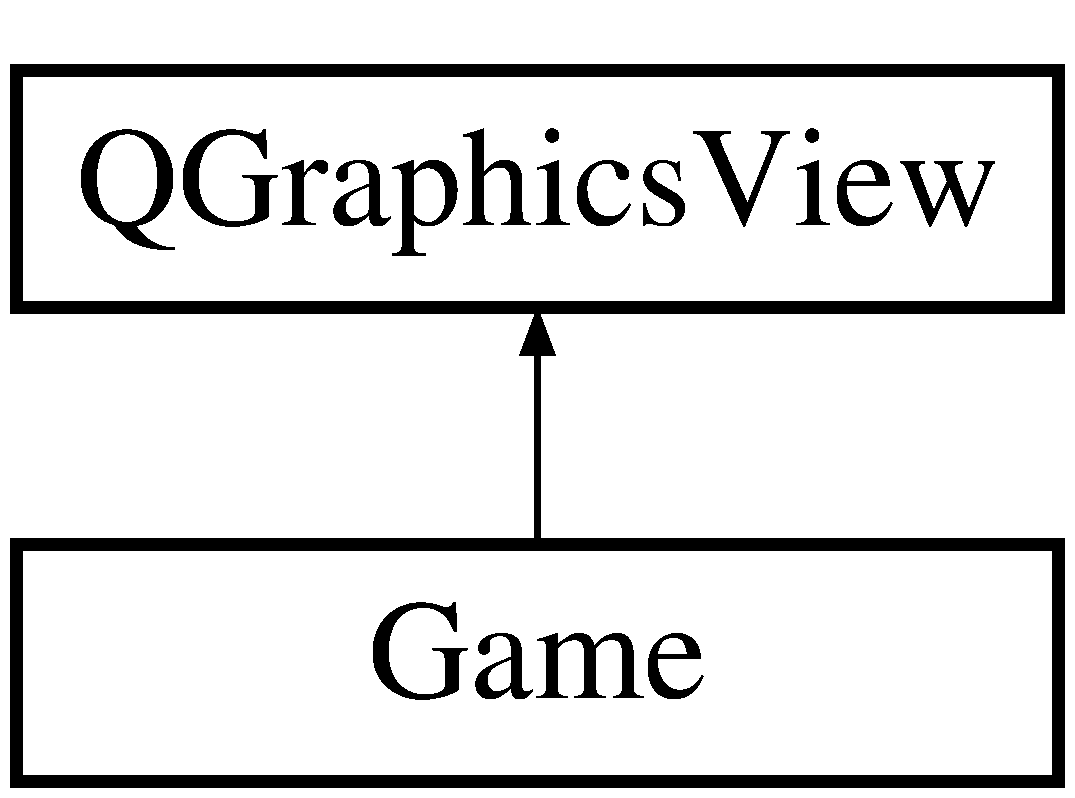
\includegraphics[height=2.000000cm]{class_game}
\end{center}
\end{figure}
\subsection*{Public Slots}
\begin{DoxyCompactItemize}
\item 
void \hyperlink{class_game_a2c06f08e42cb8ef918596edd11ee00d1}{spawn\+Enemy} (int enemy\+Num)
\item 
void \hyperlink{class_game_ad7a4181414089729ddea00c053f822c4}{spawn\+Enemy} ()
\item 
void \hyperlink{class_game_ae8638ccdb0ef3bf39a6affa30aa1258f}{start\+Game} ()
\item 
void \hyperlink{class_game_a89ee6bc4da77b30b9ab09d6148944cda}{update\+Timer} ()
\item 
void \hyperlink{class_game_a771253a0edc9a31ff64352eb0a4367cb}{wait\+Connection} ()
\item 
void \hyperlink{class_game_a480aa57ccdd02118f7716b4870a2b47c}{connection\+Established} ()
\item 
void \hyperlink{class_game_ae95e1d94393a35f3d4edda97ebfc3358}{join} ()
\end{DoxyCompactItemize}
\subsection*{Public Member Functions}
\begin{DoxyCompactItemize}
\item 
\hyperlink{class_game_ad59df6562a58a614fda24622d3715b65}{Game} ()
\item 
\hyperlink{class_game_ae3d112ca6e0e55150d2fdbc704474530}{$\sim$\+Game} ()
\item 
void \hyperlink{class_game_af74fd203e3b31917ca9d4769fa608c48}{display\+Main\+Menu} ()
\item 
void \hyperlink{class_game_a7272e282812b8af0be83044db196dc6c}{set\+Cursor} (Q\+String filename)
\item 
void \hyperlink{class_game_ad761e49ff42758930e76b477d08ba068}{mouse\+Move\+Event} (Q\+Mouse\+Event $\ast$event)
\item 
void \hyperlink{class_game_a704ba119948eebd1b6dfc547de967796}{mouse\+Press\+Event} (Q\+Mouse\+Event $\ast$event)
\item 
void \hyperlink{class_game_a622303239641db82911ea67bde3ba1a0}{create\+Enemies} (int number\+Of\+Enemies)
\item 
void \hyperlink{class_game_a838e89640d4cfbd7d7b7ee105135d4b8}{G\+A\+M\+E\+O\+V\+ER} ()
\item 
void \hyperlink{class_game_af310eb8cf154b512e2ae488267495c96}{Victory} ()
\item 
Q\+PointF \hyperlink{class_game_ae0adfbcc271a45a2c3ede2c6b948beda}{closest\+Node} (int x, int y)
\item 
void \hyperlink{class_game_a4e2cc66ce5004779048a6d8de19f0cdc}{snap\+To\+Grid} ()
\item 
void \hyperlink{class_game_a07ca125130662de9c8f3bdd2f61db9c9}{printmap} ()
\item 
void \hyperlink{class_game_aa3d45b075393d6751f77db3ce31ab9ba}{a\+\_\+star} ()
\item 
void \hyperlink{class_game_a06f5d66abdaae753db91ce7884c4e57d}{clear\+Path} ()
\item 
void \hyperlink{class_game_a065998f7609f63e2987ede928359595a}{update\+Gold} ()
\item 
void \hyperlink{class_game_aa5e4edca458d1a1378d035a138d69635}{update\+Lives} ()
\item 
void \hyperlink{class_game_a5a6924497d779286af09f339d4c7a598}{update\+Income} ()
\item 
void \hyperlink{class_game_a108f0ed818f5d32e3e5b350497edc481}{update\+Wave} ()
\end{DoxyCompactItemize}
\subsection*{Public Attributes}
\begin{DoxyCompactItemize}
\item 
bool \hyperlink{class_game_ad08e48fb0fbd89fe67ccb42ff8e8fff1}{Game\+Over} = false
\item 
Q\+Timer $\ast$ \hyperlink{class_game_a8feee9081542b15a9f2d889a6f1c8257}{gametimer}
\item 
Q\+Timer $\ast$ \hyperlink{class_game_a4774e6e02e372dabcba313802800df5d}{bullet\+Timer}
\item 
Q\+PointF \hyperlink{class_game_a861bf240380d110b285659d8af3f0406}{closest\+Node\+Pos}
\item 
Q\+Graphics\+Scene $\ast$ \hyperlink{class_game_a8119e3b9a632906c6808fa294b46a92a}{scene}
\item 
Q\+Graphics\+Pixmap\+Item $\ast$ \hyperlink{class_game_ac8bde3bd16f503846f66bbb866c3b7b9}{cursor}
\item 
\hyperlink{class_tower}{Tower} $\ast$ \hyperlink{class_game_a5917b4e021a93be7666ebc2ef4529401}{building}
\item 
Q\+Timer $\ast$ \hyperlink{class_game_a4a8895723160ca3585fe140e476aea1f}{spawntimer}
\item 
Q\+List$<$ \hyperlink{class_enemy}{Enemy} $\ast$ $>$ \hyperlink{class_game_ab96914bfc1e59035233105abfb0787fe}{list\+Of\+Enemies}
\item 
Q\+List$<$ \hyperlink{class_tower}{Tower} $\ast$ $>$ \hyperlink{class_game_aa0614c45667257e5be61685c33a2bec6}{list\+Of\+Towers}
\item 
int \hyperlink{class_game_a6ac18c388eda83ceb3212e099b3b8473}{enemies\+Spawned}
\item 
int \hyperlink{class_game_aaee1756450bae685777ee86c45ef4f78}{max\+Number\+Of\+Enemies}
\item 
int \hyperlink{class_game_ac0038cbbcfbd5d8b32600cd9f42cd09b}{enemy\+Health\+Increase} = 0
\item 
Q\+List$<$ Q\+PointF $>$ \hyperlink{class_game_abe95b23433c0353887099928a5573c59}{points\+To\+Follow}
\item 
Q\+Graphics\+Pixmap\+Item $\ast$ \hyperlink{class_game_a3b40718d348c0f12af63a3f428924ab4}{stats\+Frame}
\item 
\hyperlink{class_map}{Map} $\ast$ \hyperlink{class_game_acef3a39fdf14be2c980b0dc11e7be402}{map}
\item 
bool \hyperlink{class_game_a06579845b7a93d8bf40efe5e7592b601}{validplacement} = false
\item 
\hyperlink{class_node}{Node} $\ast$ \hyperlink{class_game_a12f4bf2a7c8503c39b3102c4cc9dd40a}{clicked\+Node}
\item 
\hyperlink{class_player1}{Player1} $\ast$ \hyperlink{class_game_ad8a7cc146f99c7ec5b7c3c25d73f118c}{player1}
\item 
Q\+Graphics\+Text\+Item $\ast$ \hyperlink{class_game_a744c42428dc6293af83752027f9cbfde}{gold\+Text}
\item 
Q\+Graphics\+Text\+Item $\ast$ \hyperlink{class_game_ab83806346d49346a645bc850c51e331c}{lives\+Text}
\item 
Q\+Graphics\+Text\+Item $\ast$ \hyperlink{class_game_a21d038c2747c61d3b5a2a3d8f1764086}{timer\+Text}
\item 
Q\+Graphics\+Text\+Item $\ast$ \hyperlink{class_game_a7d139b0ba0ef2a94966b138d5e77a034}{income\+Text}
\item 
Q\+Graphics\+Text\+Item $\ast$ \hyperlink{class_game_ac33d078835536f2dc1af85ddbabd3a20}{wave\+Text}
\item 
Q\+Graphics\+Pixmap\+Item $\ast$ \hyperlink{class_game_a1ac5cae6ba58ec5fe157b138d6c41eac}{gold\+Icon}
\item 
Q\+Graphics\+Pixmap\+Item $\ast$ \hyperlink{class_game_acd6dae5d8f0c5670fa81433f5b329e0f}{lives\+Icon}
\item 
Q\+Graphics\+Pixmap\+Item $\ast$ \hyperlink{class_game_a5853a185c9981da12d5a6330c5f121c7}{timer\+Icon}
\item 
Q\+Graphics\+Pixmap\+Item $\ast$ \hyperlink{class_game_a54671774169c28677974ee423a147c39}{income\+Icon}
\item 
Q\+Graphics\+Pixmap\+Item $\ast$ \hyperlink{class_game_ade75481ee579a63670f6d7358919634a}{wave\+Icon}
\item 
\hyperlink{class_waves}{Waves} $\ast$ \hyperlink{class_game_af9a4b49ad573785e961b29758c84fdd0}{wave}
\item 
Q\+Timer $\ast$ \hyperlink{class_game_a06a7795cf068aa5cc3b1debbea3f82ef}{wave\+Timer}
\item 
int \hyperlink{class_game_aef6faf2c7e350578fea82f340353fa6b}{timer\+Value}
\item 
\hyperlink{class_u_d_p_socket}{U\+D\+P\+Socket} $\ast$ \hyperlink{class_game_aa7fd8508fad68c550129f2be61c37467}{Client}
\item 
bool \hyperlink{class_game_aec6408b42da34f430bffb649653de96b}{connected} = false
\item 
Q\+Timer $\ast$ \hyperlink{class_game_a266d51c575b09c22aac86e20487802f4}{con\+Timer}
\item 
int \hyperlink{class_game_ab1ca40d8527bb09e773bb97030b7a5cc}{screen\+Width} = 1200
\item 
int \hyperlink{class_game_a329351d67993953391a6a65db536c017}{screen\+Height} = 1000
\item 
int \hyperlink{class_game_ad83fa5ba7b6421882d874704c7416033}{number\+Of\+Towers} = 3
\item 
int \hyperlink{class_game_af041d097dc2350360c7951e5a41bc48a}{number\+Of\+Stats} = 5
\item 
const double \hyperlink{class_game_a6c1ca48f17f6934432d01bfa7f762a04}{scalingfactor\+\_\+towers} = 0.\+28
\item 
const double \hyperlink{class_game_aeec547aa25329dcd9d52bfc1c8fa8bb3}{scalingfactor\+\_\+bullets} = 0.\+2
\item 
const double \hyperlink{class_game_a50835e7c47a3e5d6fc919ce3a163be88}{scalingfactor\+\_\+icons} = 0.\+5
\end{DoxyCompactItemize}


\subsection{Detailed Description}


Definition at line 19 of file game.\+h.



\subsection{Constructor \& Destructor Documentation}
\mbox{\Hypertarget{class_game_ad59df6562a58a614fda24622d3715b65}\label{class_game_ad59df6562a58a614fda24622d3715b65}} 
\index{Game@{Game}!Game@{Game}}
\index{Game@{Game}!Game@{Game}}
\subsubsection{\texorpdfstring{Game()}{Game()}}
{\footnotesize\ttfamily Game\+::\+Game (\begin{DoxyParamCaption}{ }\end{DoxyParamCaption})}



Definition at line 28 of file game.\+cpp.


\begin{DoxyCode}
29 \{
30     \textcolor{comment}{//create a scene}
31     \hyperlink{class_game_a8119e3b9a632906c6808fa294b46a92a}{scene} = \textcolor{keyword}{new} QGraphicsScene(\textcolor{keyword}{this});
32     \hyperlink{class_game_a8119e3b9a632906c6808fa294b46a92a}{scene}->setSceneRect(0,0,\hyperlink{class_game_ab1ca40d8527bb09e773bb97030b7a5cc}{screenWidth},\hyperlink{class_game_a329351d67993953391a6a65db536c017}{screenHeight});
33     \hyperlink{class_game_a8119e3b9a632906c6808fa294b46a92a}{scene}->setBackgroundBrush(QBrush(QColor(213,173,81),Qt::Dense3Pattern));
34 
35     \textcolor{comment}{//set the scene}
36     setScene(\hyperlink{class_game_a8119e3b9a632906c6808fa294b46a92a}{scene});
37 \textcolor{comment}{//    setDragMode(QGraphicsView::ScrollHandDrag);}
38 
39     \textcolor{comment}{//alter window}
40     setMinimumSize(\hyperlink{class_game_ab1ca40d8527bb09e773bb97030b7a5cc}{screenWidth},\hyperlink{class_game_a329351d67993953391a6a65db536c017}{screenHeight});
41     setHorizontalScrollBarPolicy(Qt::ScrollBarAlwaysOff);
42     setVerticalScrollBarPolicy(Qt::ScrollBarAlwaysOff);
43 
44     \textcolor{comment}{//set cursor}
45     \hyperlink{class_game_ac8bde3bd16f503846f66bbb866c3b7b9}{cursor} = \textcolor{keyword}{nullptr};
46     \hyperlink{class_game_a5917b4e021a93be7666ebc2ef4529401}{building} = \textcolor{keyword}{nullptr};
47     setMouseTracking(\textcolor{keyword}{true});
48 
49 
50     \textcolor{comment}{//create map}
51     \hyperlink{class_game_acef3a39fdf14be2c980b0dc11e7be402}{map} = \textcolor{keyword}{new} \hyperlink{class_map}{Map}();
52     \hyperlink{class_game_af9a4b49ad573785e961b29758c84fdd0}{wave} = \textcolor{keyword}{new} \hyperlink{class_waves}{Waves}();
53 
54     \textcolor{comment}{//make game timer}
55     \hyperlink{class_game_a8feee9081542b15a9f2d889a6f1c8257}{gametimer} = \textcolor{keyword}{new} QTimer(\textcolor{keyword}{this});
56     \hyperlink{class_game_a8feee9081542b15a9f2d889a6f1c8257}{gametimer}->start(150);
57 
58     \textcolor{comment}{//make bullet timer}
59     \hyperlink{class_game_a4774e6e02e372dabcba313802800df5d}{bulletTimer} = \textcolor{keyword}{new} QTimer(\textcolor{keyword}{this});
60     \hyperlink{class_game_a4774e6e02e372dabcba313802800df5d}{bulletTimer}->start(50);
61 
62 \}
\end{DoxyCode}
\mbox{\Hypertarget{class_game_ae3d112ca6e0e55150d2fdbc704474530}\label{class_game_ae3d112ca6e0e55150d2fdbc704474530}} 
\index{Game@{Game}!````~Game@{$\sim$\+Game}}
\index{````~Game@{$\sim$\+Game}!Game@{Game}}
\subsubsection{\texorpdfstring{$\sim$\+Game()}{~Game()}}
{\footnotesize\ttfamily Game\+::$\sim$\+Game (\begin{DoxyParamCaption}{ }\end{DoxyParamCaption})}



Definition at line 64 of file game.\+cpp.


\begin{DoxyCode}
65 \{
66 
67 \}
\end{DoxyCode}


\subsection{Member Function Documentation}
\mbox{\Hypertarget{class_game_aa3d45b075393d6751f77db3ce31ab9ba}\label{class_game_aa3d45b075393d6751f77db3ce31ab9ba}} 
\index{Game@{Game}!a\+\_\+star@{a\+\_\+star}}
\index{a\+\_\+star@{a\+\_\+star}!Game@{Game}}
\subsubsection{\texorpdfstring{a\+\_\+star()}{a\_star()}}
{\footnotesize\ttfamily void Game\+::a\+\_\+star (\begin{DoxyParamCaption}{ }\end{DoxyParamCaption})}



Definition at line 459 of file game.\+cpp.


\begin{DoxyCode}
460 \{
461     \hyperlink{class_game_abe95b23433c0353887099928a5573c59}{pointsToFollow}.clear();
462     \hyperlink{class_game_acef3a39fdf14be2c980b0dc11e7be402}{map}->\hyperlink{class_map_ab19ca30427e7257d713f5fcfa0ac1a10}{openList}.clear();
463     \hyperlink{class_game_acef3a39fdf14be2c980b0dc11e7be402}{map}->\hyperlink{class_map_ae1ced58b787598940bb444659bacd7d3}{closedList}.clear();
464 
465     \hyperlink{class_game_acef3a39fdf14be2c980b0dc11e7be402}{map}->\hyperlink{class_map_ae1ced58b787598940bb444659bacd7d3}{closedList}.append(\hyperlink{class_game_acef3a39fdf14be2c980b0dc11e7be402}{map}->\hyperlink{class_map_aafcbf6f458eb48f4945f3d0b58d2ef85}{start});
466     \hyperlink{class_game_acef3a39fdf14be2c980b0dc11e7be402}{map}->\hyperlink{class_map_adac9fc32a2c840b40e1417292e846fe2}{calcNeighbours}(\hyperlink{class_game_acef3a39fdf14be2c980b0dc11e7be402}{map}->\hyperlink{class_map_aafcbf6f458eb48f4945f3d0b58d2ef85}{start});
467 
468     \textcolor{keywordflow}{while} (\hyperlink{class_game_acef3a39fdf14be2c980b0dc11e7be402}{map}->\hyperlink{class_map_ab19ca30427e7257d713f5fcfa0ac1a10}{openList}.length() > 0)
469     \{
470         \hyperlink{class_node}{Node} *t = \hyperlink{class_game_acef3a39fdf14be2c980b0dc11e7be402}{map}->\hyperlink{class_map_a19461c64e6da374e8022d210a6930867}{smallestF}();
471         \hyperlink{class_game_acef3a39fdf14be2c980b0dc11e7be402}{map}->\hyperlink{class_map_ae1ced58b787598940bb444659bacd7d3}{closedList}.append(t);
472         \textcolor{keywordflow}{if} (t == \hyperlink{class_game_acef3a39fdf14be2c980b0dc11e7be402}{map}->\hyperlink{class_map_abdb357cb53c27be3b6e3c2b54bfde669}{finish})
473         \{
474             \textcolor{keywordflow}{while} (t->\hyperlink{class_node_ad8184598cdea70e4bbdfd76f2b0f9e85}{parent})
475             \{
476                 t->\hyperlink{class_node_a2bb1959485873369ea2504c1dece3f33}{path} = \textcolor{keyword}{true};
477                 t = t->\hyperlink{class_node_ad8184598cdea70e4bbdfd76f2b0f9e85}{parent};
478                 t->\hyperlink{class_node_a2250e2c1710fb19f15f236ac69563613}{tile} = \hyperlink{node_8h_ac9e486ec80ccfdb28a4f4837d419c9f1a064af96be640396afe6970cc3cffba4c}{Path};
479                 \hyperlink{class_game_abe95b23433c0353887099928a5573c59}{pointsToFollow}.prepend(t->\hyperlink{class_node_a77faa088c74e20a361a181b58e8a4c7f}{point});
480                 \hyperlink{class_game_abe95b23433c0353887099928a5573c59}{pointsToFollow}.append(\hyperlink{class_game_acef3a39fdf14be2c980b0dc11e7be402}{map}->\hyperlink{class_map_abdb357cb53c27be3b6e3c2b54bfde669}{finish}->\hyperlink{class_node_a77faa088c74e20a361a181b58e8a4c7f}{point});
481                 \hyperlink{class_game_a06579845b7a93d8bf40efe5e7592b601}{validplacement} = \textcolor{keyword}{true};
482             \}
483 
484         \}
485         \hyperlink{class_game_acef3a39fdf14be2c980b0dc11e7be402}{map}->\hyperlink{class_map_adac9fc32a2c840b40e1417292e846fe2}{calcNeighbours}(t);
486     \}
487 \}
\end{DoxyCode}
\mbox{\Hypertarget{class_game_a06f5d66abdaae753db91ce7884c4e57d}\label{class_game_a06f5d66abdaae753db91ce7884c4e57d}} 
\index{Game@{Game}!clear\+Path@{clear\+Path}}
\index{clear\+Path@{clear\+Path}!Game@{Game}}
\subsubsection{\texorpdfstring{clear\+Path()}{clearPath()}}
{\footnotesize\ttfamily void Game\+::clear\+Path (\begin{DoxyParamCaption}{ }\end{DoxyParamCaption})}



Definition at line 489 of file game.\+cpp.


\begin{DoxyCode}
490 \{
491     \textcolor{keywordflow}{for} (\textcolor{keywordtype}{int} i = 0; i < \hyperlink{class_game_acef3a39fdf14be2c980b0dc11e7be402}{map}->\hyperlink{class_map_acfd20721da29a2e353598555e23e12f0}{mapX}; ++i) \{
492         \textcolor{keywordflow}{for} (\textcolor{keywordtype}{int} j = \hyperlink{class_game_acef3a39fdf14be2c980b0dc11e7be402}{map}->\hyperlink{class_map_ae08efae9ac1453b2690985c627aca358}{mapY} -1; j >= 0; --j) \{
493             \hyperlink{class_game_acef3a39fdf14be2c980b0dc11e7be402}{map}->\hyperlink{class_map_a7298e7a7b5dbdc642c49ded9a2c754a5}{map}[i][j]->\hyperlink{class_node_aff1029a518bdc2651007b8856f958364}{x} = i;
494             \hyperlink{class_game_acef3a39fdf14be2c980b0dc11e7be402}{map}->\hyperlink{class_map_a7298e7a7b5dbdc642c49ded9a2c754a5}{map}[i][j]->\hyperlink{class_node_aa3e5b5240023b4528ae85057b3324202}{y} = j;
495             \hyperlink{class_game_acef3a39fdf14be2c980b0dc11e7be402}{map}->\hyperlink{class_map_a7298e7a7b5dbdc642c49ded9a2c754a5}{map}[i][j]->\hyperlink{class_node_a32fbe9e0f4fc9e9d1845ce808738d7ab}{f} = 0;
496             \hyperlink{class_game_acef3a39fdf14be2c980b0dc11e7be402}{map}->\hyperlink{class_map_a7298e7a7b5dbdc642c49ded9a2c754a5}{map}[i][j]->\hyperlink{class_node_a0b249888eacdec6c623ec8c58b230c48}{g} = 0;
497             \hyperlink{class_game_acef3a39fdf14be2c980b0dc11e7be402}{map}->\hyperlink{class_map_a7298e7a7b5dbdc642c49ded9a2c754a5}{map}[i][j]->\hyperlink{class_node_afb5a7ac7536a9e09488bb685420cd78a}{h} = 0;
498             \hyperlink{class_game_acef3a39fdf14be2c980b0dc11e7be402}{map}->\hyperlink{class_map_a7298e7a7b5dbdc642c49ded9a2c754a5}{map}[i][j]->\hyperlink{class_node_ad8184598cdea70e4bbdfd76f2b0f9e85}{parent} = 0;
499             \textcolor{keywordflow}{if} (\hyperlink{class_game_acef3a39fdf14be2c980b0dc11e7be402}{map}->\hyperlink{class_map_a7298e7a7b5dbdc642c49ded9a2c754a5}{map}[i][j]->\hyperlink{class_node_a2250e2c1710fb19f15f236ac69563613}{tile} == \hyperlink{node_8h_ac9e486ec80ccfdb28a4f4837d419c9f1a064af96be640396afe6970cc3cffba4c}{Path}) \{
500                 \hyperlink{class_game_acef3a39fdf14be2c980b0dc11e7be402}{map}->\hyperlink{class_map_a7298e7a7b5dbdc642c49ded9a2c754a5}{map}[i][j]->\hyperlink{class_node_a2250e2c1710fb19f15f236ac69563613}{tile} = \hyperlink{node_8h_ac9e486ec80ccfdb28a4f4837d419c9f1a283b79b5e51a79e202e0702f189485ad}{Grass};
501             \}
502             \hyperlink{class_game_acef3a39fdf14be2c980b0dc11e7be402}{map}->\hyperlink{class_map_a7298e7a7b5dbdc642c49ded9a2c754a5}{map}[i][j]->\hyperlink{class_node_a2bb1959485873369ea2504c1dece3f33}{path} = \textcolor{keyword}{false};
503         \}
504     \}
505 \}
\end{DoxyCode}
\mbox{\Hypertarget{class_game_ae0adfbcc271a45a2c3ede2c6b948beda}\label{class_game_ae0adfbcc271a45a2c3ede2c6b948beda}} 
\index{Game@{Game}!closest\+Node@{closest\+Node}}
\index{closest\+Node@{closest\+Node}!Game@{Game}}
\subsubsection{\texorpdfstring{closest\+Node()}{closestNode()}}
{\footnotesize\ttfamily Q\+PointF Game\+::closest\+Node (\begin{DoxyParamCaption}\item[{int}]{x,  }\item[{int}]{y }\end{DoxyParamCaption})}



Definition at line 292 of file game.\+cpp.


\begin{DoxyCode}
293 \{
294     QList<QPointF> nodelist = \hyperlink{class_game_acef3a39fdf14be2c980b0dc11e7be402}{map}->\hyperlink{class_map_a07f51de84c133707fedaeffd04aff2d5}{nodepoints};
295     \textcolor{keywordtype}{double} distance\_old = 10000;
296     QPointF closestPoint;
297 
298     QListIterator<QPointF> i(nodelist);
299     \textcolor{keywordflow}{while} (i.hasNext()) \{
300         QPointF nextpoint = i.next();
301         QLineF ln(QPointF(x,y),nextpoint);
302         \textcolor{keywordtype}{double} distance\_new = ln.length();
303         \textcolor{keywordflow}{if} (distance\_new<=distance\_old) \{
304             distance\_old = distance\_new;
305             \hyperlink{class_game_a861bf240380d110b285659d8af3f0406}{closestNodePos} = nextpoint;
306 
307         \}
308     \}
309     \textcolor{keywordflow}{return} closestPoint;
310 \}
\end{DoxyCode}
\mbox{\Hypertarget{class_game_a480aa57ccdd02118f7716b4870a2b47c}\label{class_game_a480aa57ccdd02118f7716b4870a2b47c}} 
\index{Game@{Game}!connection\+Established@{connection\+Established}}
\index{connection\+Established@{connection\+Established}!Game@{Game}}
\subsubsection{\texorpdfstring{connection\+Established}{connectionEstablished}}
{\footnotesize\ttfamily void Game\+::connection\+Established (\begin{DoxyParamCaption}{ }\end{DoxyParamCaption})\hspace{0.3cm}{\ttfamily [slot]}}



Definition at line 582 of file game.\+cpp.


\begin{DoxyCode}
583 \{  
584     \textcolor{keywordflow}{if} (\hyperlink{class_game_aec6408b42da34f430bffb649653de96b}{connected} == \textcolor{keyword}{true}) \{
585         \textcolor{comment}{//qDebug() << Host->hostAdress;}
586         \hyperlink{class_game_ae8638ccdb0ef3bf39a6affa30aa1258f}{startGame}();
587         \hyperlink{class_game_aec6408b42da34f430bffb649653de96b}{connected} = \textcolor{keyword}{false};
588         \hyperlink{class_game_a266d51c575b09c22aac86e20487802f4}{conTimer}->disconnect();
589     \}
590 \}
\end{DoxyCode}
\mbox{\Hypertarget{class_game_a622303239641db82911ea67bde3ba1a0}\label{class_game_a622303239641db82911ea67bde3ba1a0}} 
\index{Game@{Game}!create\+Enemies@{create\+Enemies}}
\index{create\+Enemies@{create\+Enemies}!Game@{Game}}
\subsubsection{\texorpdfstring{create\+Enemies()}{createEnemies()}}
{\footnotesize\ttfamily void Game\+::create\+Enemies (\begin{DoxyParamCaption}\item[{int}]{number\+Of\+Enemies }\end{DoxyParamCaption})}



Definition at line 179 of file game.\+cpp.


\begin{DoxyCode}
180 \{
181     \hyperlink{class_game_a6ac18c388eda83ceb3212e099b3b8473}{enemiesSpawned} = 0;
182     \hyperlink{class_game_aaee1756450bae685777ee86c45ef4f78}{maxNumberOfEnemies} = numberOfEnemies;
183     connect(\hyperlink{class_game_a4a8895723160ca3585fe140e476aea1f}{spawntimer}, SIGNAL(timeout()), \textcolor{keyword}{this}, SLOT(\hyperlink{class_game_ad7a4181414089729ddea00c053f822c4}{spawnEnemy}()));
184     \hyperlink{class_game_a4a8895723160ca3585fe140e476aea1f}{spawntimer}->start(1000);
185 \}
\end{DoxyCode}
\mbox{\Hypertarget{class_game_af74fd203e3b31917ca9d4769fa608c48}\label{class_game_af74fd203e3b31917ca9d4769fa608c48}} 
\index{Game@{Game}!display\+Main\+Menu@{display\+Main\+Menu}}
\index{display\+Main\+Menu@{display\+Main\+Menu}!Game@{Game}}
\subsubsection{\texorpdfstring{display\+Main\+Menu()}{displayMainMenu()}}
{\footnotesize\ttfamily void Game\+::display\+Main\+Menu (\begin{DoxyParamCaption}{ }\end{DoxyParamCaption})}



Definition at line 69 of file game.\+cpp.


\begin{DoxyCode}
70 \{
71     \textcolor{comment}{//create brackground}
72     QGraphicsPixmapItem *backgroundImage = \textcolor{keyword}{new} QGraphicsPixmapItem;
73     backgroundImage->setPixmap(QString(\textcolor{stringliteral}{":/images/images/test.png"}));
74     backgroundImage->setScale(1);
75     backgroundImage->setPos(-375,-200);
76     \hyperlink{class_game_a8119e3b9a632906c6808fa294b46a92a}{scene}->addItem(backgroundImage);
77 
78     \textcolor{comment}{//create the title text}
79     QGraphicsTextItem *titleText = \textcolor{keyword}{new} QGraphicsTextItem(QString(\textcolor{stringliteral}{"Element Tower Defense"}));
80     QFont titleFont(\textcolor{stringliteral}{"Pixel Emulator"}, 40);
81     titleText->setFont(titleFont);
82     titleText->setDefaultTextColor(QColor(\textcolor{stringliteral}{"white"}));
83     \textcolor{keywordtype}{int} txpos = this->width()/2 - titleText->boundingRect().width()/2;
84     \textcolor{keywordtype}{int} typos = 200;
85     titleText->setPos(txpos,typos);
86     \hyperlink{class_game_a8119e3b9a632906c6808fa294b46a92a}{scene}->addItem(titleText);
87 
88     \textcolor{comment}{//create play button}
89     \hyperlink{class_button}{Button} *playbutton = \textcolor{keyword}{new} \hyperlink{class_button}{Button}(QString(\textcolor{stringliteral}{"Play"}));
90     \textcolor{keywordtype}{int} bxPos = this->width()/2 - playbutton->boundingRect().width()/2;
91     \textcolor{keywordtype}{int} byPos = 500;
92     playbutton->setPos(bxPos,byPos);
93     connect(playbutton,SIGNAL(clicked()), \textcolor{keyword}{this}, SLOT(\hyperlink{class_game_ae8638ccdb0ef3bf39a6affa30aa1258f}{startGame}()));
94     \hyperlink{class_game_a8119e3b9a632906c6808fa294b46a92a}{scene}->addItem(playbutton);
95 
96     \textcolor{comment}{//create host button}
97     \hyperlink{class_button}{Button} *hostbutton = \textcolor{keyword}{new} \hyperlink{class_button}{Button}(QString(\textcolor{stringliteral}{"Host"}));
98     \textcolor{keywordtype}{int} hxPos = this->width()/3 - playbutton->boundingRect().width()/2;
99     \textcolor{keywordtype}{int} hyPos = 650;
100     hostbutton->setPos(hxPos,hyPos);
101     connect(hostbutton,SIGNAL(clicked()), \textcolor{keyword}{this}, SLOT(\hyperlink{class_game_a771253a0edc9a31ff64352eb0a4367cb}{waitConnection}()));
102     \hyperlink{class_game_a8119e3b9a632906c6808fa294b46a92a}{scene}->addItem(hostbutton);
103 
104     \textcolor{comment}{//create join button}
105     \hyperlink{class_button}{Button} *joinbutton = \textcolor{keyword}{new} \hyperlink{class_button}{Button}(QString(\textcolor{stringliteral}{"Join"}));
106     \textcolor{keywordtype}{int} jxPos = this->width()/3*2 - playbutton->boundingRect().width()/2;
107     \textcolor{keywordtype}{int} jyPos = 650;
108     joinbutton->setPos(jxPos,jyPos);
109     connect(joinbutton,SIGNAL(clicked()), \textcolor{keyword}{this}, SLOT(\hyperlink{class_game_ae95e1d94393a35f3d4edda97ebfc3358}{join}()));
110     \hyperlink{class_game_a8119e3b9a632906c6808fa294b46a92a}{scene}->addItem(joinbutton);
111 
112     \textcolor{comment}{//create quit button}
113     \hyperlink{class_button}{Button} *quitbutton = \textcolor{keyword}{new} \hyperlink{class_button}{Button}(QString(\textcolor{stringliteral}{"Quit"}));
114     \textcolor{keywordtype}{int} qxPos = this->width()/2 - quitbutton->boundingRect().width()/2;
115     \textcolor{keywordtype}{int} qyPos = 800;
116     quitbutton->setPos(qxPos,qyPos);
117     connect(quitbutton, SIGNAL(clicked()), \textcolor{keyword}{this}, SLOT(close()));
118     \hyperlink{class_game_a8119e3b9a632906c6808fa294b46a92a}{scene}->addItem(quitbutton);
119 
120 
121     \textcolor{comment}{//setup network test code}
122     \textcolor{comment}{//Host = new UDPSocket(this);}
123     \hyperlink{class_game_aa7fd8508fad68c550129f2be61c37467}{Client} = \textcolor{keyword}{new} \hyperlink{class_u_d_p_socket}{UDPSocket}(\textcolor{keyword}{this});
124     \hyperlink{class_game_aa7fd8508fad68c550129f2be61c37467}{Client}->\hyperlink{class_u_d_p_socket_a5bdac3040e57d37c503fdd3293b6d053}{setHostAdress}(QHostAddress::LocalHost); \textcolor{comment}{//default is loopback address}
125     \textcolor{comment}{//Host->setHostAdress(QHostAddress::LocalHost); //default is loopback address}
126 
127 
128 \}
\end{DoxyCode}
\mbox{\Hypertarget{class_game_a838e89640d4cfbd7d7b7ee105135d4b8}\label{class_game_a838e89640d4cfbd7d7b7ee105135d4b8}} 
\index{Game@{Game}!G\+A\+M\+E\+O\+V\+ER@{G\+A\+M\+E\+O\+V\+ER}}
\index{G\+A\+M\+E\+O\+V\+ER@{G\+A\+M\+E\+O\+V\+ER}!Game@{Game}}
\subsubsection{\texorpdfstring{G\+A\+M\+E\+O\+V\+E\+R()}{GAMEOVER()}}
{\footnotesize\ttfamily void Game\+::\+G\+A\+M\+E\+O\+V\+ER (\begin{DoxyParamCaption}{ }\end{DoxyParamCaption})}



Definition at line 187 of file game.\+cpp.


\begin{DoxyCode}
188 \{  
189     \textcolor{comment}{//stuur Game over oor netwerk}
190     \hyperlink{class_game_aa7fd8508fad68c550129f2be61c37467}{Client}->\hyperlink{class_u_d_p_socket_a66a6c4663cc3084cb4d76583e8039083}{send}(\textcolor{stringliteral}{"GO"});
191 
192 
193     \textcolor{comment}{//disconnects timer}
194     \hyperlink{class_game_a06a7795cf068aa5cc3b1debbea3f82ef}{waveTimer}->disconnect();
195     \hyperlink{class_game_a8feee9081542b15a9f2d889a6f1c8257}{gametimer}->disconnect();
196 
197 
198 
199     QListIterator<Enemy *> i(\hyperlink{class_game_ab96914bfc1e59035233105abfb0787fe}{listOfEnemies});
200     \textcolor{keywordflow}{while} (i.hasNext()) \{
201         \hyperlink{class_enemy}{Enemy} *thisEnemy = i.next();
202         \textcolor{comment}{//thisEnemy->timer->disconnect(); //gee crash}
203         thisEnemy->deleteLater();
204     \}
205 
206 
207     \textcolor{comment}{//delete towers}
208     QListIterator<Tower*> j(\hyperlink{class_game_aa0614c45667257e5be61685c33a2bec6}{listOfTowers});
209     \textcolor{keywordflow}{while} (j.hasNext()) \{
210         \hyperlink{class_tower}{Tower} *thisTower = j.next();
211         thisTower->deleteLater();
212     \}
213 
214     qDebug() << \textcolor{stringliteral}{"wup wup wup!"};
215     QMessageBox msgBox;
216     msgBox.setText(\textcolor{stringliteral}{"Defeat!"});
217     msgBox.setInformativeText(\textcolor{stringliteral}{"Restart?"});
218     msgBox.setStandardButtons(QMessageBox::Ok | QMessageBox::Close);
219     msgBox.setDefaultButton(QMessageBox::Ok);
220     \textcolor{keywordtype}{int} ret = msgBox.exec();
221 
222     \textcolor{keywordflow}{switch} (ret) \{
223     \textcolor{keywordflow}{case} QMessageBox::Ok:
224         \textcolor{comment}{// restart clicked}
225 
226 
227         \hyperlink{class_game_af74fd203e3b31917ca9d4769fa608c48}{displayMainMenu}();
228         \textcolor{keywordflow}{break};
229     \textcolor{keywordflow}{case} QMessageBox::Close:
230         \textcolor{comment}{// close clicked}
231         close();
232         \textcolor{keywordflow}{break};
233 
234     \textcolor{keywordflow}{default}:
235         \textcolor{comment}{// should never be reached}
236         close();
237         \textcolor{keywordflow}{break};
238     \}
239 \}
\end{DoxyCode}
\mbox{\Hypertarget{class_game_ae95e1d94393a35f3d4edda97ebfc3358}\label{class_game_ae95e1d94393a35f3d4edda97ebfc3358}} 
\index{Game@{Game}!join@{join}}
\index{join@{join}!Game@{Game}}
\subsubsection{\texorpdfstring{join}{join}}
{\footnotesize\ttfamily void Game\+::join (\begin{DoxyParamCaption}{ }\end{DoxyParamCaption})\hspace{0.3cm}{\ttfamily [slot]}}



Definition at line 592 of file game.\+cpp.


\begin{DoxyCode}
593 \{
594     \textcolor{keywordtype}{bool} ok;
595     QString text = QInputDialog::getText(\textcolor{keyword}{this}, tr(\textcolor{stringliteral}{"Join"}),
596                                          tr(\textcolor{stringliteral}{"Host IP Address: "}), QLineEdit::Normal, \textcolor{stringliteral}{"127.0.0.1"} , &ok);
597     \textcolor{keywordflow}{if} (ok) \{
598         \hyperlink{class_game_aa7fd8508fad68c550129f2be61c37467}{Client}->\hyperlink{class_u_d_p_socket_aacd808913633488ab008e8aa7ff8d9cf}{hostAdress} = QHostAddress(text);
599         \hyperlink{class_game_aa7fd8508fad68c550129f2be61c37467}{Client}->\hyperlink{class_u_d_p_socket_a66a6c4663cc3084cb4d76583e8039083}{send}(\textcolor{stringliteral}{"ACK"});
600         \hyperlink{class_game_ae8638ccdb0ef3bf39a6affa30aa1258f}{startGame}();
601     \}
602 
603 \}
\end{DoxyCode}
\mbox{\Hypertarget{class_game_ad761e49ff42758930e76b477d08ba068}\label{class_game_ad761e49ff42758930e76b477d08ba068}} 
\index{Game@{Game}!mouse\+Move\+Event@{mouse\+Move\+Event}}
\index{mouse\+Move\+Event@{mouse\+Move\+Event}!Game@{Game}}
\subsubsection{\texorpdfstring{mouse\+Move\+Event()}{mouseMoveEvent()}}
{\footnotesize\ttfamily void Game\+::mouse\+Move\+Event (\begin{DoxyParamCaption}\item[{Q\+Mouse\+Event $\ast$}]{event }\end{DoxyParamCaption})}



Definition at line 148 of file game.\+cpp.


\begin{DoxyCode}
149 \{
150     \textcolor{keywordflow}{if} (\hyperlink{class_game_ac8bde3bd16f503846f66bbb866c3b7b9}{cursor}) \{
151         \textcolor{keywordtype}{int} pos\_mouse\_x = \textcolor{keyword}{event}->pos().x();
152         \textcolor{keywordtype}{int} pos\_mouse\_y = \textcolor{keyword}{event}->pos().y();
153         \hyperlink{class_game_ac8bde3bd16f503846f66bbb866c3b7b9}{cursor}->setPos(pos\_mouse\_x,pos\_mouse\_y);
154     \}
155 \}
\end{DoxyCode}
\mbox{\Hypertarget{class_game_a704ba119948eebd1b6dfc547de967796}\label{class_game_a704ba119948eebd1b6dfc547de967796}} 
\index{Game@{Game}!mouse\+Press\+Event@{mouse\+Press\+Event}}
\index{mouse\+Press\+Event@{mouse\+Press\+Event}!Game@{Game}}
\subsubsection{\texorpdfstring{mouse\+Press\+Event()}{mousePressEvent()}}
{\footnotesize\ttfamily void Game\+::mouse\+Press\+Event (\begin{DoxyParamCaption}\item[{Q\+Mouse\+Event $\ast$}]{event }\end{DoxyParamCaption})}



Definition at line 157 of file game.\+cpp.


\begin{DoxyCode}
158 \{
159     \textcolor{comment}{//if we are building}
160     \textcolor{keywordflow}{if} (\hyperlink{class_game_a5917b4e021a93be7666ebc2ef4529401}{building}) \{
161 
162         \hyperlink{class_game_a06f5d66abdaae753db91ce7884c4e57d}{clearPath}();
163         \hyperlink{class_game_ae0adfbcc271a45a2c3ede2c6b948beda}{closestNode}(event->pos().x(),\textcolor{keyword}{event}->pos().y());
164         \hyperlink{class_game_a4e2cc66ce5004779048a6d8de19f0cdc}{snapToGrid}();
165 
166         \textcolor{comment}{//re initialize variables}
167         \textcolor{keyword}{delete} \hyperlink{class_game_ac8bde3bd16f503846f66bbb866c3b7b9}{cursor};
168         \hyperlink{class_game_ac8bde3bd16f503846f66bbb866c3b7b9}{cursor} = \textcolor{keyword}{nullptr};
169         \hyperlink{class_game_a5917b4e021a93be7666ebc2ef4529401}{building} = \textcolor{keyword}{nullptr};
170         \hyperlink{class_game_a06579845b7a93d8bf40efe5e7592b601}{validplacement} = \textcolor{keyword}{false};
171 
172     \}
173     \textcolor{keywordflow}{else}
174     \{
175         QGraphicsView::mousePressEvent(event);
176     \}
177 \}
\end{DoxyCode}
\mbox{\Hypertarget{class_game_a07ca125130662de9c8f3bdd2f61db9c9}\label{class_game_a07ca125130662de9c8f3bdd2f61db9c9}} 
\index{Game@{Game}!printmap@{printmap}}
\index{printmap@{printmap}!Game@{Game}}
\subsubsection{\texorpdfstring{printmap()}{printmap()}}
{\footnotesize\ttfamily void Game\+::printmap (\begin{DoxyParamCaption}{ }\end{DoxyParamCaption})}



Definition at line 381 of file game.\+cpp.


\begin{DoxyCode}
382 \{
383     \textcolor{comment}{//print map}
384     \textcolor{keywordflow}{for} (\textcolor{keywordtype}{int} i = 0; i < \hyperlink{class_game_acef3a39fdf14be2c980b0dc11e7be402}{map}->\hyperlink{class_map_acfd20721da29a2e353598555e23e12f0}{mapX}; ++i)
385     \{
386         \textcolor{keywordflow}{for} (\textcolor{keywordtype}{int} j = \hyperlink{class_game_acef3a39fdf14be2c980b0dc11e7be402}{map}->\hyperlink{class_map_ae08efae9ac1453b2690985c627aca358}{mapY} -1; j >= 0; --j)
387         \{
388             \hyperlink{class_node}{Node} *l = \textcolor{keyword}{new} \hyperlink{class_node}{Node}();
389             \textcolor{keywordflow}{switch}(\hyperlink{class_game_acef3a39fdf14be2c980b0dc11e7be402}{map}->\hyperlink{class_map_a7298e7a7b5dbdc642c49ded9a2c754a5}{map}[i][j]->\hyperlink{class_node_a2250e2c1710fb19f15f236ac69563613}{tile})
390             \{
391             \textcolor{keywordflow}{case} \hyperlink{node_8h_ac9e486ec80ccfdb28a4f4837d419c9f1a283b79b5e51a79e202e0702f189485ad}{Grass}:\textcolor{comment}{//or portal}
392                 \textcolor{keywordflow}{if} (((i==\hyperlink{class_game_acef3a39fdf14be2c980b0dc11e7be402}{map}->\hyperlink{class_map_acfd20721da29a2e353598555e23e12f0}{mapX}/2)&&(j==0))||((i==\hyperlink{class_game_acef3a39fdf14be2c980b0dc11e7be402}{map}->\hyperlink{class_map_acfd20721da29a2e353598555e23e12f0}{mapX}/2)&&(j==
      \hyperlink{class_game_acef3a39fdf14be2c980b0dc11e7be402}{map}->\hyperlink{class_map_ae08efae9ac1453b2690985c627aca358}{mapY}-1))) \{
393                     l->setPixmap(*\hyperlink{class_game_acef3a39fdf14be2c980b0dc11e7be402}{map}->\hyperlink{class_map_a4dafaf125d6014a97e98168e41492cd5}{portal});
394                 \}
395                 \textcolor{keywordflow}{else}
396                 \{
397                     l->setPixmap(*\hyperlink{class_game_acef3a39fdf14be2c980b0dc11e7be402}{map}->\hyperlink{class_map_a322ef8e3f55269ef565a58f20190d148}{grass});
398                 \}
399                 \textcolor{keywordflow}{break};
400             \textcolor{keywordflow}{case} \hyperlink{node_8h_ac9e486ec80ccfdb28a4f4837d419c9f1a064af96be640396afe6970cc3cffba4c}{Path}:
401                 l->setPixmap(*\hyperlink{class_game_acef3a39fdf14be2c980b0dc11e7be402}{map}->\hyperlink{class_map_a99d78bd384bf091660dbc6e1123419b0}{path});
402                 \textcolor{keywordflow}{break};
403             \textcolor{keywordflow}{case} \hyperlink{node_8h_ac9e486ec80ccfdb28a4f4837d419c9f1ae4afc87ae4a7816fdef8d05002e6dce4}{Obstruction}:\textcolor{comment}{//or edges}
404                 \textcolor{comment}{//if top edge}
405                 \textcolor{keywordflow}{if} ((i>0)&&(i<map->mapX-1)&&(j==0)) \{
406                     l->setPixmap(QPixmap(\textcolor{stringliteral}{":/images/images/mapTile\_007.png"}));
407                 \}
408                 \textcolor{comment}{//if bottom edge}
409                 \textcolor{keywordflow}{else} \textcolor{keywordflow}{if} ((i>0)&&(i<map->mapX-1)&&(j==\hyperlink{class_game_acef3a39fdf14be2c980b0dc11e7be402}{map}->\hyperlink{class_map_ae08efae9ac1453b2690985c627aca358}{mapY}-1)) \{
410                     l->setPixmap(QPixmap(\textcolor{stringliteral}{":/images/images/mapTile\_052.png"}));
411                 \}
412                 \textcolor{comment}{//if left edge}
413                 \textcolor{keywordflow}{else} \textcolor{keywordflow}{if} ((i==0)&&(j>0)&&(j<map->mapY-1)) \{
414                     l->setPixmap(QPixmap(\textcolor{stringliteral}{":/images/images/mapTile\_021.png"}));
415                 \}
416                 \textcolor{comment}{//if right edge}
417                 \textcolor{keywordflow}{else} \textcolor{keywordflow}{if} ((i==\hyperlink{class_game_acef3a39fdf14be2c980b0dc11e7be402}{map}->\hyperlink{class_map_acfd20721da29a2e353598555e23e12f0}{mapX}-1)&&(j>0)&&(j<map->mapY-1)) \{
418                     l->setPixmap(QPixmap(\textcolor{stringliteral}{":/images/images/mapTile\_023.png"}));
419                 \}
420                 \textcolor{comment}{//if top left corner}
421                 \textcolor{keywordflow}{else} \textcolor{keywordflow}{if} ((i==0)&&(j==0))
422                 \{
423                     l->setPixmap(QPixmap(\textcolor{stringliteral}{":/images/images/mapTile\_006.png"}));
424                 \}
425                 \textcolor{comment}{//if top right corner}
426                 \textcolor{keywordflow}{else} \textcolor{keywordflow}{if} ((i==\hyperlink{class_game_acef3a39fdf14be2c980b0dc11e7be402}{map}->\hyperlink{class_map_acfd20721da29a2e353598555e23e12f0}{mapX}-1)&&(j==0))
427                 \{
428                     l->setPixmap(QPixmap(\textcolor{stringliteral}{":/images/images/mapTile\_008.png"}));
429                 \}
430 
431                 \textcolor{comment}{//if bottom left corner}
432                 \textcolor{keywordflow}{else} \textcolor{keywordflow}{if} ((i==0)&&(j==\hyperlink{class_game_acef3a39fdf14be2c980b0dc11e7be402}{map}->\hyperlink{class_map_ae08efae9ac1453b2690985c627aca358}{mapY}-1))
433                 \{
434                     l->setPixmap(QPixmap(\textcolor{stringliteral}{":/images/images/mapTile\_051.png"}));
435                 \}
436 
437                 \textcolor{comment}{//if bottom right corner}
438                 \textcolor{keywordflow}{else} \textcolor{keywordflow}{if} ((i==\hyperlink{class_game_acef3a39fdf14be2c980b0dc11e7be402}{map}->\hyperlink{class_map_acfd20721da29a2e353598555e23e12f0}{mapX}-1)&&(j==\hyperlink{class_game_acef3a39fdf14be2c980b0dc11e7be402}{map}->\hyperlink{class_map_ae08efae9ac1453b2690985c627aca358}{mapY}-1))
439                 \{
440                     l->setPixmap(QPixmap(\textcolor{stringliteral}{":/images/images/mapTile\_053.png"}));
441                 \}
442                 \textcolor{keywordflow}{else}
443                 \{
444                     l->setPixmap(*\hyperlink{class_game_acef3a39fdf14be2c980b0dc11e7be402}{map}->\hyperlink{class_map_af0167137084000cfb58a33df8474bcbe}{obstruction});
445                 \}
446                 \textcolor{keywordflow}{break};
447             \}
448             \textcolor{keywordtype}{int} x = i * \hyperlink{class_game_acef3a39fdf14be2c980b0dc11e7be402}{map}->\hyperlink{class_map_af2aa425dd22aba483ae973c4a15fe934}{tileX};
449             \textcolor{keywordtype}{int} y = j * \hyperlink{class_game_acef3a39fdf14be2c980b0dc11e7be402}{map}->\hyperlink{class_map_a483dfba507cee9d2fa60a074992b1fcf}{tileY};
450             \hyperlink{class_game_a8119e3b9a632906c6808fa294b46a92a}{scene}->addItem(l);
451             l->setPos(x,y);
452             l->setZValue(-1);
453 
454 
455         \}
456     \}
457 \}
\end{DoxyCode}
\mbox{\Hypertarget{class_game_a7272e282812b8af0be83044db196dc6c}\label{class_game_a7272e282812b8af0be83044db196dc6c}} 
\index{Game@{Game}!set\+Cursor@{set\+Cursor}}
\index{set\+Cursor@{set\+Cursor}!Game@{Game}}
\subsubsection{\texorpdfstring{set\+Cursor()}{setCursor()}}
{\footnotesize\ttfamily void Game\+::set\+Cursor (\begin{DoxyParamCaption}\item[{Q\+String}]{filename }\end{DoxyParamCaption})}



Definition at line 130 of file game.\+cpp.


\begin{DoxyCode}
131 \{
132     \textcolor{comment}{//creates the building before placing}
133     \textcolor{keywordflow}{if} (\hyperlink{class_game_ac8bde3bd16f503846f66bbb866c3b7b9}{cursor}) \{
134         \hyperlink{class_game_a8119e3b9a632906c6808fa294b46a92a}{scene}->removeItem(\hyperlink{class_game_ac8bde3bd16f503846f66bbb866c3b7b9}{cursor});
135         \textcolor{comment}{//delete cursor; //remove die?}
136     \}
137     \hyperlink{class_game_ac8bde3bd16f503846f66bbb866c3b7b9}{cursor} = \textcolor{keyword}{new} QGraphicsPixmapItem();
138     \hyperlink{class_game_ac8bde3bd16f503846f66bbb866c3b7b9}{cursor}->setPixmap(QPixmap(filename));
139 
140     \textcolor{keywordtype}{int} w = \hyperlink{class_game_ac8bde3bd16f503846f66bbb866c3b7b9}{cursor}->pixmap().width();
141     \textcolor{keywordtype}{int} h = \hyperlink{class_game_ac8bde3bd16f503846f66bbb866c3b7b9}{cursor}->pixmap().height();
142     \hyperlink{class_game_ac8bde3bd16f503846f66bbb866c3b7b9}{cursor}->setOffset(-w/2,-h/1.25);
143     \hyperlink{class_game_ac8bde3bd16f503846f66bbb866c3b7b9}{cursor}->setScale(\hyperlink{class_game_a6c1ca48f17f6934432d01bfa7f762a04}{scalingfactor\_towers});
144 
145     \hyperlink{class_game_a8119e3b9a632906c6808fa294b46a92a}{scene}->addItem(\hyperlink{class_game_ac8bde3bd16f503846f66bbb866c3b7b9}{cursor});
146 \}
\end{DoxyCode}
\mbox{\Hypertarget{class_game_a4e2cc66ce5004779048a6d8de19f0cdc}\label{class_game_a4e2cc66ce5004779048a6d8de19f0cdc}} 
\index{Game@{Game}!snap\+To\+Grid@{snap\+To\+Grid}}
\index{snap\+To\+Grid@{snap\+To\+Grid}!Game@{Game}}
\subsubsection{\texorpdfstring{snap\+To\+Grid()}{snapToGrid()}}
{\footnotesize\ttfamily void Game\+::snap\+To\+Grid (\begin{DoxyParamCaption}{ }\end{DoxyParamCaption})}



Definition at line 314 of file game.\+cpp.


\begin{DoxyCode}
315 \{
316 
317     \hyperlink{class_game_a06579845b7a93d8bf40efe5e7592b601}{validplacement} = \textcolor{keyword}{false};
318 
319     \textcolor{comment}{//clicked node}
320     \textcolor{keywordtype}{int} x\_map = (\hyperlink{class_game_a861bf240380d110b285659d8af3f0406}{closestNodePos}.x() -\hyperlink{class_game_acef3a39fdf14be2c980b0dc11e7be402}{map}->\hyperlink{class_map_af2aa425dd22aba483ae973c4a15fe934}{tileX}/2)/\hyperlink{class_game_acef3a39fdf14be2c980b0dc11e7be402}{map}->
      \hyperlink{class_map_af2aa425dd22aba483ae973c4a15fe934}{tileX};
321     \textcolor{keywordtype}{int} y\_map = (\hyperlink{class_game_a861bf240380d110b285659d8af3f0406}{closestNodePos}.y() -\hyperlink{class_game_acef3a39fdf14be2c980b0dc11e7be402}{map}->\hyperlink{class_map_a483dfba507cee9d2fa60a074992b1fcf}{tileY}/2)/\hyperlink{class_game_acef3a39fdf14be2c980b0dc11e7be402}{map}->
      \hyperlink{class_map_a483dfba507cee9d2fa60a074992b1fcf}{tileY};
322     \hyperlink{class_game_a12f4bf2a7c8503c39b3102c4cc9dd40a}{clickedNode} = \textcolor{keyword}{new} \hyperlink{class_node}{Node}();
323     \hyperlink{class_game_a12f4bf2a7c8503c39b3102c4cc9dd40a}{clickedNode} = \hyperlink{class_game_acef3a39fdf14be2c980b0dc11e7be402}{map}->\hyperlink{class_map_a9500f43b02ce38b5e89248bd6e257858}{getNode}(x\_map,y\_map);
324 
325 
326     \textcolor{comment}{//if it is already a obstruction return}
327     \textcolor{keywordflow}{if} (\hyperlink{class_game_a12f4bf2a7c8503c39b3102c4cc9dd40a}{clickedNode}->\hyperlink{class_node_a2250e2c1710fb19f15f236ac69563613}{tile} == \hyperlink{node_8h_ac9e486ec80ccfdb28a4f4837d419c9f1ae4afc87ae4a7816fdef8d05002e6dce4}{Obstruction}) \{
328         \textcolor{keywordflow}{return};
329     \}
330     \textcolor{keywordflow}{else}
331     \{
332 
333         \hyperlink{class_game_ad8a7cc146f99c7ec5b7c3c25d73f118c}{player1}->\hyperlink{class_player1_ab390478b345e443398bac442a04b675c}{Gold} += -\hyperlink{class_game_a5917b4e021a93be7666ebc2ef4529401}{building}->\hyperlink{class_tower_ae1d3f44d0149c8146ccf6b262a52ddad}{getCostOfTower}();
334         \textcolor{comment}{//if enough gold place tower}
335         \textcolor{keywordflow}{if} (\hyperlink{class_game_ad8a7cc146f99c7ec5b7c3c25d73f118c}{player1}->\hyperlink{class_player1_a9395a16fecb7b96395455f096ac1b60b}{getGold}() >= 0) \{
336             \textcolor{comment}{// otherwise, build at the clicked location}
337             \hyperlink{class_game_a065998f7609f63e2987ede928359595a}{updateGold}();
338 
339 
340             \hyperlink{class_game_a12f4bf2a7c8503c39b3102c4cc9dd40a}{clickedNode}->\hyperlink{class_node_a2250e2c1710fb19f15f236ac69563613}{tile} = \hyperlink{node_8h_ac9e486ec80ccfdb28a4f4837d419c9f1ae4afc87ae4a7816fdef8d05002e6dce4}{Obstruction};
341             \textcolor{comment}{//set map node here}
342             \hyperlink{class_game_acef3a39fdf14be2c980b0dc11e7be402}{map}->\hyperlink{class_map_a7298e7a7b5dbdc642c49ded9a2c754a5}{map}[x\_map][y\_map]->\hyperlink{class_node_a2250e2c1710fb19f15f236ac69563613}{tile} = \hyperlink{node_8h_ac9e486ec80ccfdb28a4f4837d419c9f1ae4afc87ae4a7816fdef8d05002e6dce4}{Obstruction};
343             \hyperlink{class_game_acef3a39fdf14be2c980b0dc11e7be402}{map}->\hyperlink{class_map_a7298e7a7b5dbdc642c49ded9a2c754a5}{map}[x\_map][y\_map]->\hyperlink{class_node_aae24f318bd4b6d14270084cec3fc98b5}{cost} = 100;
344 
345             \textcolor{comment}{//run pathfinding}
346             \hyperlink{class_game_aa3d45b075393d6751f77db3ce31ab9ba}{a\_star}();
347             \textcolor{keywordflow}{if} (\hyperlink{class_game_a06579845b7a93d8bf40efe5e7592b601}{validplacement} == \textcolor{keyword}{true}) \{
348                 \hyperlink{class_game_aa3d45b075393d6751f77db3ce31ab9ba}{a\_star}();
349                 \hyperlink{class_game_a07ca125130662de9c8f3bdd2f61db9c9}{printmap}();
350                 \hyperlink{class_game_a8119e3b9a632906c6808fa294b46a92a}{scene}->addItem(\hyperlink{class_game_a5917b4e021a93be7666ebc2ef4529401}{building});
351                 \hyperlink{class_game_aa0614c45667257e5be61685c33a2bec6}{listOfTowers}.append(\hyperlink{class_game_a5917b4e021a93be7666ebc2ef4529401}{building});
352                 \hyperlink{class_game_a5917b4e021a93be7666ebc2ef4529401}{building}->setPos(\hyperlink{class_game_a861bf240380d110b285659d8af3f0406}{closestNodePos});
353                 \hyperlink{class_game_a5917b4e021a93be7666ebc2ef4529401}{building}->setScale(\hyperlink{class_game_a6c1ca48f17f6934432d01bfa7f762a04}{scalingfactor\_towers});
354                 \hyperlink{class_game_a5917b4e021a93be7666ebc2ef4529401}{building}->setZValue(y\_map);
355             \}
356             \textcolor{keywordflow}{else}
357             \{
358                 \hyperlink{class_game_a12f4bf2a7c8503c39b3102c4cc9dd40a}{clickedNode}->\hyperlink{class_node_a2250e2c1710fb19f15f236ac69563613}{tile} = \hyperlink{node_8h_ac9e486ec80ccfdb28a4f4837d419c9f1a283b79b5e51a79e202e0702f189485ad}{Grass};
359                 \textcolor{comment}{//set map node here}
360                 \hyperlink{class_game_acef3a39fdf14be2c980b0dc11e7be402}{map}->\hyperlink{class_map_a7298e7a7b5dbdc642c49ded9a2c754a5}{map}[x\_map][y\_map]->\hyperlink{class_node_a2250e2c1710fb19f15f236ac69563613}{tile} = \hyperlink{node_8h_ac9e486ec80ccfdb28a4f4837d419c9f1a283b79b5e51a79e202e0702f189485ad}{Grass};
361                 \hyperlink{class_game_acef3a39fdf14be2c980b0dc11e7be402}{map}->\hyperlink{class_map_a7298e7a7b5dbdc642c49ded9a2c754a5}{map}[x\_map][y\_map]->\hyperlink{class_node_aae24f318bd4b6d14270084cec3fc98b5}{cost} = 1;
362                 \hyperlink{class_game_aa3d45b075393d6751f77db3ce31ab9ba}{a\_star}();
363                 \hyperlink{class_game_ad8a7cc146f99c7ec5b7c3c25d73f118c}{player1}->\hyperlink{class_player1_ab390478b345e443398bac442a04b675c}{Gold} += \hyperlink{class_game_a5917b4e021a93be7666ebc2ef4529401}{building}->\hyperlink{class_tower_ae1d3f44d0149c8146ccf6b262a52ddad}{getCostOfTower}();
364                 \hyperlink{class_game_a065998f7609f63e2987ede928359595a}{updateGold}();
365                 \textcolor{keywordflow}{return};
366 
367             \}
368         \}
369         \textcolor{keywordflow}{else}
370         \{
371             \hyperlink{class_game_ad8a7cc146f99c7ec5b7c3c25d73f118c}{player1}->\hyperlink{class_player1_ab390478b345e443398bac442a04b675c}{Gold} += \hyperlink{class_game_a5917b4e021a93be7666ebc2ef4529401}{building}->\hyperlink{class_tower_ae1d3f44d0149c8146ccf6b262a52ddad}{getCostOfTower}();
372             \hyperlink{class_game_a065998f7609f63e2987ede928359595a}{updateGold}();
373             \textcolor{keywordflow}{return};
374         \}
375     \}
376 
377 \}
\end{DoxyCode}
\mbox{\Hypertarget{class_game_a2c06f08e42cb8ef918596edd11ee00d1}\label{class_game_a2c06f08e42cb8ef918596edd11ee00d1}} 
\index{Game@{Game}!spawn\+Enemy@{spawn\+Enemy}}
\index{spawn\+Enemy@{spawn\+Enemy}!Game@{Game}}
\subsubsection{\texorpdfstring{spawn\+Enemy}{spawnEnemy}\hspace{0.1cm}{\footnotesize\ttfamily [1/2]}}
{\footnotesize\ttfamily void Game\+::spawn\+Enemy (\begin{DoxyParamCaption}\item[{int}]{enemy\+Num }\end{DoxyParamCaption})\hspace{0.3cm}{\ttfamily [slot]}}



Definition at line 621 of file game.\+cpp.


\begin{DoxyCode}
622 \{
623     \textcolor{comment}{//spawn and enemy}
624     \hyperlink{class_enemy}{Enemy} *enemy = \textcolor{keyword}{new} \hyperlink{class_enemy}{Enemy}(\hyperlink{class_game_abe95b23433c0353887099928a5573c59}{pointsToFollow}, enemyNum);
625     enemy->\hyperlink{class_enemy_aedd5e7bf8ef07ee97be433c853a10d8d}{health} += \hyperlink{class_game_ac0038cbbcfbd5d8b32600cd9f42cd09b}{enemyHealthIncrease};
626     \hyperlink{class_game_ab96914bfc1e59035233105abfb0787fe}{listOfEnemies} << enemy;
627     enemy->setPos(\hyperlink{class_game_abe95b23433c0353887099928a5573c59}{pointsToFollow}[0]);
628     \hyperlink{class_game_a8119e3b9a632906c6808fa294b46a92a}{scene}->addItem(enemy);
629     \hyperlink{class_game_a6ac18c388eda83ceb3212e099b3b8473}{enemiesSpawned} += 1;
630 
631     \textcolor{keywordflow}{if} (\hyperlink{class_game_a6ac18c388eda83ceb3212e099b3b8473}{enemiesSpawned} >= \hyperlink{class_game_aaee1756450bae685777ee86c45ef4f78}{maxNumberOfEnemies}) \{
632         \hyperlink{class_game_a4a8895723160ca3585fe140e476aea1f}{spawntimer}->disconnect();
633     \}
634 \}
\end{DoxyCode}
\mbox{\Hypertarget{class_game_ad7a4181414089729ddea00c053f822c4}\label{class_game_ad7a4181414089729ddea00c053f822c4}} 
\index{Game@{Game}!spawn\+Enemy@{spawn\+Enemy}}
\index{spawn\+Enemy@{spawn\+Enemy}!Game@{Game}}
\subsubsection{\texorpdfstring{spawn\+Enemy}{spawnEnemy}\hspace{0.1cm}{\footnotesize\ttfamily [2/2]}}
{\footnotesize\ttfamily void Game\+::spawn\+Enemy (\begin{DoxyParamCaption}{ }\end{DoxyParamCaption})\hspace{0.3cm}{\ttfamily [slot]}}



Definition at line 606 of file game.\+cpp.


\begin{DoxyCode}
607 \{
608     \textcolor{comment}{//spawn and enemy}
609     \hyperlink{class_enemy}{Enemy} *enemy = \textcolor{keyword}{new} \hyperlink{class_enemy}{Enemy}(\hyperlink{class_game_abe95b23433c0353887099928a5573c59}{pointsToFollow}, 1);
610     enemy->\hyperlink{class_enemy_aedd5e7bf8ef07ee97be433c853a10d8d}{health} += \hyperlink{class_game_ac0038cbbcfbd5d8b32600cd9f42cd09b}{enemyHealthIncrease};
611     \hyperlink{class_game_ab96914bfc1e59035233105abfb0787fe}{listOfEnemies} << enemy;
612     enemy->setPos(\hyperlink{class_game_abe95b23433c0353887099928a5573c59}{pointsToFollow}[0]);
613     \hyperlink{class_game_a8119e3b9a632906c6808fa294b46a92a}{scene}->addItem(enemy);
614     \hyperlink{class_game_a6ac18c388eda83ceb3212e099b3b8473}{enemiesSpawned} += 1;
615 
616     \textcolor{keywordflow}{if} (\hyperlink{class_game_a6ac18c388eda83ceb3212e099b3b8473}{enemiesSpawned} >= \hyperlink{class_game_aaee1756450bae685777ee86c45ef4f78}{maxNumberOfEnemies}) \{
617         \hyperlink{class_game_a4a8895723160ca3585fe140e476aea1f}{spawntimer}->disconnect();
618     \}
619 \}
\end{DoxyCode}
\mbox{\Hypertarget{class_game_ae8638ccdb0ef3bf39a6affa30aa1258f}\label{class_game_ae8638ccdb0ef3bf39a6affa30aa1258f}} 
\index{Game@{Game}!start\+Game@{start\+Game}}
\index{start\+Game@{start\+Game}!Game@{Game}}
\subsubsection{\texorpdfstring{start\+Game}{startGame}}
{\footnotesize\ttfamily void Game\+::start\+Game (\begin{DoxyParamCaption}{ }\end{DoxyParamCaption})\hspace{0.3cm}{\ttfamily [slot]}}

{\itshape add building frame}/ 

Definition at line 637 of file game.\+cpp.


\begin{DoxyCode}
638 \{
639     \textcolor{comment}{//clear the screen}
640     \hyperlink{class_game_a8119e3b9a632906c6808fa294b46a92a}{scene}->clear();
641 
642     \textcolor{comment}{/*create game instance*/}
643     \textcolor{comment}{//set cursor}
644     \hyperlink{class_game_ac8bde3bd16f503846f66bbb866c3b7b9}{cursor} = \textcolor{keyword}{nullptr};
645     \hyperlink{class_game_a5917b4e021a93be7666ebc2ef4529401}{building} = \textcolor{keyword}{nullptr};
646     setMouseTracking(\textcolor{keyword}{true});
647 
648     \textcolor{comment}{//create map}
649     \hyperlink{class_game_acef3a39fdf14be2c980b0dc11e7be402}{map} = \textcolor{keyword}{new} \hyperlink{class_map}{Map}();
650     \hyperlink{class_game_a06579845b7a93d8bf40efe5e7592b601}{validplacement} = \textcolor{keyword}{false};
651     \hyperlink{class_game_aa3d45b075393d6751f77db3ce31ab9ba}{a\_star}();
652     \hyperlink{class_game_a07ca125130662de9c8f3bdd2f61db9c9}{printmap}();
653 
654     \textcolor{comment}{//initialize player1}
655     \hyperlink{class_game_ad8a7cc146f99c7ec5b7c3c25d73f118c}{player1} = \textcolor{keyword}{new} \hyperlink{class_player1}{Player1};
656 
657 
658     \textcolor{comment}{//create enemy initialize}
659     \hyperlink{class_game_a4a8895723160ca3585fe140e476aea1f}{spawntimer} = \textcolor{keyword}{new} QTimer(\textcolor{keyword}{this});
660     \hyperlink{class_game_a6ac18c388eda83ceb3212e099b3b8473}{enemiesSpawned} = 0;
661     \hyperlink{class_game_aaee1756450bae685777ee86c45ef4f78}{maxNumberOfEnemies} = 0;
662 
663     \textcolor{comment}{//add stats bar}
664     \hyperlink{class_game_a3b40718d348c0f12af63a3f428924ab4}{statsFrame} = \textcolor{keyword}{new} QGraphicsPixmapItem();
665     \hyperlink{class_game_a3b40718d348c0f12af63a3f428924ab4}{statsFrame}->setPixmap(QString(\textcolor{stringliteral}{":/images/images/frame3.png"}));
666     \textcolor{keywordtype}{double} framescale = 0.72;
667     \hyperlink{class_game_a3b40718d348c0f12af63a3f428924ab4}{statsFrame}->setScale(framescale);
668     \hyperlink{class_game_a3b40718d348c0f12af63a3f428924ab4}{statsFrame}->setPos(\hyperlink{class_game_acef3a39fdf14be2c980b0dc11e7be402}{map}->\hyperlink{class_map_acfd20721da29a2e353598555e23e12f0}{mapX}*\hyperlink{class_game_acef3a39fdf14be2c980b0dc11e7be402}{map}->\hyperlink{class_map_af2aa425dd22aba483ae973c4a15fe934}{tileX}+15,50);
669     \hyperlink{class_game_a3b40718d348c0f12af63a3f428924ab4}{statsFrame}->setZValue(-1);
670     \hyperlink{class_game_a8119e3b9a632906c6808fa294b46a92a}{scene}->addItem(\hyperlink{class_game_a3b40718d348c0f12af63a3f428924ab4}{statsFrame});
671 
672     \textcolor{comment}{/*add stats*/}
673     \textcolor{comment}{//gold frame}
674     \hyperlink{class_game_a1ac5cae6ba58ec5fe157b138d6c41eac}{goldIcon} = \textcolor{keyword}{new} QGraphicsPixmapItem();
675     \hyperlink{class_game_a1ac5cae6ba58ec5fe157b138d6c41eac}{goldIcon}->setPixmap(QString(\textcolor{stringliteral}{":/images/images/gold.png"}));
676     \textcolor{keywordtype}{int} xgoldPos = \hyperlink{class_game_acef3a39fdf14be2c980b0dc11e7be402}{map}->\hyperlink{class_map_acfd20721da29a2e353598555e23e12f0}{mapX}*\hyperlink{class_game_acef3a39fdf14be2c980b0dc11e7be402}{map}->\hyperlink{class_map_af2aa425dd22aba483ae973c4a15fe934}{tileX} + \hyperlink{class_game_acef3a39fdf14be2c980b0dc11e7be402}{map}->\hyperlink{class_map_af2aa425dd22aba483ae973c4a15fe934}{tileX}+ 15;
677     \textcolor{keywordtype}{int} ygoldPos = \hyperlink{class_game_a3b40718d348c0f12af63a3f428924ab4}{statsFrame}->pixmap().height()*framescale/(
      \hyperlink{class_game_af041d097dc2350360c7951e5a41bc48a}{numberOfStats}+1) +10;
678     \textcolor{keywordtype}{double} goldscale = 0.45;
679     \hyperlink{class_game_a1ac5cae6ba58ec5fe157b138d6c41eac}{goldIcon}->setPos(xgoldPos,ygoldPos);
680     \hyperlink{class_game_a1ac5cae6ba58ec5fe157b138d6c41eac}{goldIcon}->setScale(goldscale);
681     \hyperlink{class_game_a1ac5cae6ba58ec5fe157b138d6c41eac}{goldIcon}->setZValue(0);
682     \hyperlink{class_game_a8119e3b9a632906c6808fa294b46a92a}{scene}->addItem(\hyperlink{class_game_a1ac5cae6ba58ec5fe157b138d6c41eac}{goldIcon});
683     \textcolor{comment}{//add text info}
684     \hyperlink{class_game_a744c42428dc6293af83752027f9cbfde}{goldText} = \textcolor{keyword}{new} QGraphicsTextItem(QString::number(\hyperlink{class_game_ad8a7cc146f99c7ec5b7c3c25d73f118c}{player1}->
      \hyperlink{class_player1_a9395a16fecb7b96395455f096ac1b60b}{getGold}()));
685     QFont goldFont(\textcolor{stringliteral}{"Pixel Emulator"}, 14);
686     \hyperlink{class_game_a744c42428dc6293af83752027f9cbfde}{goldText}->setFont(goldFont);
687     \hyperlink{class_game_a744c42428dc6293af83752027f9cbfde}{goldText}->setDefaultTextColor(QColor(\textcolor{stringliteral}{"white"}));
688     \textcolor{keywordtype}{int} txgpos = xgoldPos + \hyperlink{class_game_a1ac5cae6ba58ec5fe157b138d6c41eac}{goldIcon}->pixmap().width()/3*goldscale + 5;
689     \textcolor{keywordtype}{int} tygpos = ygoldPos +10;
690     \hyperlink{class_game_a744c42428dc6293af83752027f9cbfde}{goldText}->setPos(txgpos,tygpos);
691     \hyperlink{class_game_a8119e3b9a632906c6808fa294b46a92a}{scene}->addItem(\hyperlink{class_game_a744c42428dc6293af83752027f9cbfde}{goldText});
692 
693 
694     \textcolor{comment}{//lives}
695     \hyperlink{class_game_acd6dae5d8f0c5670fa81433f5b329e0f}{livesIcon} = \textcolor{keyword}{new} QGraphicsPixmapItem();
696     \hyperlink{class_game_acd6dae5d8f0c5670fa81433f5b329e0f}{livesIcon}->setPixmap(QString(\textcolor{stringliteral}{":/images/images/lives.png"}));
697     xgoldPos = \hyperlink{class_game_acef3a39fdf14be2c980b0dc11e7be402}{map}->\hyperlink{class_map_acfd20721da29a2e353598555e23e12f0}{mapX}*\hyperlink{class_game_acef3a39fdf14be2c980b0dc11e7be402}{map}->\hyperlink{class_map_af2aa425dd22aba483ae973c4a15fe934}{tileX} + \hyperlink{class_game_acef3a39fdf14be2c980b0dc11e7be402}{map}->\hyperlink{class_map_af2aa425dd22aba483ae973c4a15fe934}{tileX}+ 15;
698     ygoldPos = \hyperlink{class_game_a3b40718d348c0f12af63a3f428924ab4}{statsFrame}->pixmap().height()*framescale/(\hyperlink{class_game_af041d097dc2350360c7951e5a41bc48a}{numberOfStats}+1)*2 +10;
699     \hyperlink{class_game_acd6dae5d8f0c5670fa81433f5b329e0f}{livesIcon}->setPos(xgoldPos,ygoldPos);
700     \hyperlink{class_game_acd6dae5d8f0c5670fa81433f5b329e0f}{livesIcon}->setScale(0.45);
701     \hyperlink{class_game_acd6dae5d8f0c5670fa81433f5b329e0f}{livesIcon}->setZValue(0);
702     \hyperlink{class_game_a8119e3b9a632906c6808fa294b46a92a}{scene}->addItem(\hyperlink{class_game_acd6dae5d8f0c5670fa81433f5b329e0f}{livesIcon});
703     \textcolor{comment}{//add lives info}
704     \hyperlink{class_game_ab83806346d49346a645bc850c51e331c}{livesText} = \textcolor{keyword}{new} QGraphicsTextItem(QString::number(\hyperlink{class_game_ad8a7cc146f99c7ec5b7c3c25d73f118c}{player1}->
      \hyperlink{class_player1_afb2adc7bd83c6380fbb85a832e083f4d}{getLives}()));
705     QFont livesFont(\textcolor{stringliteral}{"Pixel Emulator"}, 14);
706     \hyperlink{class_game_ab83806346d49346a645bc850c51e331c}{livesText}->setFont(livesFont);
707     \hyperlink{class_game_ab83806346d49346a645bc850c51e331c}{livesText}->setDefaultTextColor(QColor(\textcolor{stringliteral}{"white"}));
708     \textcolor{keywordtype}{int} txlpos = xgoldPos + \hyperlink{class_game_acd6dae5d8f0c5670fa81433f5b329e0f}{livesIcon}->pixmap().width()/3*0.55 + 5;
709     \textcolor{keywordtype}{int} tylpos = ygoldPos +10;
710     \hyperlink{class_game_ab83806346d49346a645bc850c51e331c}{livesText}->setPos(txlpos,tylpos);
711     \hyperlink{class_game_a8119e3b9a632906c6808fa294b46a92a}{scene}->addItem(\hyperlink{class_game_ab83806346d49346a645bc850c51e331c}{livesText});
712 
713     \textcolor{comment}{//start timer}
714     \hyperlink{class_game_a06a7795cf068aa5cc3b1debbea3f82ef}{waveTimer} = \textcolor{keyword}{new} QTimer(\textcolor{keyword}{this});
715     connect(\hyperlink{class_game_a06a7795cf068aa5cc3b1debbea3f82ef}{waveTimer}, SIGNAL(timeout()), \textcolor{keyword}{this}, SLOT(\hyperlink{class_game_a89ee6bc4da77b30b9ab09d6148944cda}{updateTimer}()));
716     \hyperlink{class_game_a06a7795cf068aa5cc3b1debbea3f82ef}{waveTimer}->start(1000);
717 
718     \textcolor{comment}{//wave timers}
719     \hyperlink{class_game_a5853a185c9981da12d5a6330c5f121c7}{timerIcon} = \textcolor{keyword}{new} QGraphicsPixmapItem();
720     \hyperlink{class_game_a5853a185c9981da12d5a6330c5f121c7}{timerIcon}->setPixmap(QString(\textcolor{stringliteral}{":/images/images/timer.png"}));
721     xgoldPos = \hyperlink{class_game_acef3a39fdf14be2c980b0dc11e7be402}{map}->\hyperlink{class_map_acfd20721da29a2e353598555e23e12f0}{mapX}*\hyperlink{class_game_acef3a39fdf14be2c980b0dc11e7be402}{map}->\hyperlink{class_map_af2aa425dd22aba483ae973c4a15fe934}{tileX} + \hyperlink{class_game_acef3a39fdf14be2c980b0dc11e7be402}{map}->\hyperlink{class_map_af2aa425dd22aba483ae973c4a15fe934}{tileX}+ 15;
722     ygoldPos = \hyperlink{class_game_a3b40718d348c0f12af63a3f428924ab4}{statsFrame}->pixmap().height()*framescale/(\hyperlink{class_game_af041d097dc2350360c7951e5a41bc48a}{numberOfStats}+1)*3 +10;
723     \hyperlink{class_game_a5853a185c9981da12d5a6330c5f121c7}{timerIcon}->setPos(xgoldPos,ygoldPos);
724     \hyperlink{class_game_a5853a185c9981da12d5a6330c5f121c7}{timerIcon}->setScale(0.45);
725     \hyperlink{class_game_a5853a185c9981da12d5a6330c5f121c7}{timerIcon}->setZValue(0);
726     \hyperlink{class_game_a8119e3b9a632906c6808fa294b46a92a}{scene}->addItem(\hyperlink{class_game_a5853a185c9981da12d5a6330c5f121c7}{timerIcon});
727     \textcolor{comment}{//add timer info}
728     \hyperlink{class_game_aef6faf2c7e350578fea82f340353fa6b}{timerValue} = 45;
729     \hyperlink{class_game_a21d038c2747c61d3b5a2a3d8f1764086}{timerText} = \textcolor{keyword}{new} QGraphicsTextItem(QString::number(\hyperlink{class_game_aef6faf2c7e350578fea82f340353fa6b}{timerValue}));
730     QFont timerFont(\textcolor{stringliteral}{"Pixel Emulator"}, 14);
731     \hyperlink{class_game_a21d038c2747c61d3b5a2a3d8f1764086}{timerText}->setFont(timerFont);
732     \hyperlink{class_game_a21d038c2747c61d3b5a2a3d8f1764086}{timerText}->setDefaultTextColor(QColor(\textcolor{stringliteral}{"white"}));
733     \textcolor{keywordtype}{int} txtpos = xgoldPos + \hyperlink{class_game_a5853a185c9981da12d5a6330c5f121c7}{timerIcon}->pixmap().width()*0.6*0.55 + 5;
734     \textcolor{keywordtype}{int} tytpos = ygoldPos +10;
735     \hyperlink{class_game_a21d038c2747c61d3b5a2a3d8f1764086}{timerText}->setPos(txtpos,tytpos);
736     \hyperlink{class_game_a8119e3b9a632906c6808fa294b46a92a}{scene}->addItem(\hyperlink{class_game_a21d038c2747c61d3b5a2a3d8f1764086}{timerText});
737 
738     \textcolor{comment}{//income}
739     \hyperlink{class_game_a54671774169c28677974ee423a147c39}{incomeIcon} = \textcolor{keyword}{new} QGraphicsPixmapItem();
740     \hyperlink{class_game_a54671774169c28677974ee423a147c39}{incomeIcon}->setPixmap(QString(\textcolor{stringliteral}{":/images/images/income.png"}));
741     xgoldPos = \hyperlink{class_game_acef3a39fdf14be2c980b0dc11e7be402}{map}->\hyperlink{class_map_acfd20721da29a2e353598555e23e12f0}{mapX}*\hyperlink{class_game_acef3a39fdf14be2c980b0dc11e7be402}{map}->\hyperlink{class_map_af2aa425dd22aba483ae973c4a15fe934}{tileX} + \hyperlink{class_game_acef3a39fdf14be2c980b0dc11e7be402}{map}->\hyperlink{class_map_af2aa425dd22aba483ae973c4a15fe934}{tileX}+ 15;
742     ygoldPos = \hyperlink{class_game_a3b40718d348c0f12af63a3f428924ab4}{statsFrame}->pixmap().height()*framescale/(\hyperlink{class_game_af041d097dc2350360c7951e5a41bc48a}{numberOfStats}+1)*4 +10;
743     \hyperlink{class_game_a54671774169c28677974ee423a147c39}{incomeIcon}->setPos(xgoldPos,ygoldPos);
744     \textcolor{keywordtype}{double} incomeScale = 0.42;
745     \hyperlink{class_game_a54671774169c28677974ee423a147c39}{incomeIcon}->setScale(incomeScale);
746     \hyperlink{class_game_a54671774169c28677974ee423a147c39}{incomeIcon}->setZValue(0);
747     \hyperlink{class_game_a8119e3b9a632906c6808fa294b46a92a}{scene}->addItem(\hyperlink{class_game_a54671774169c28677974ee423a147c39}{incomeIcon});
748     \textcolor{comment}{//add income info}
749     \hyperlink{class_game_a7d139b0ba0ef2a94966b138d5e77a034}{incomeText} = \textcolor{keyword}{new} QGraphicsTextItem(QString::number(\hyperlink{class_game_ad8a7cc146f99c7ec5b7c3c25d73f118c}{player1}->
      \hyperlink{class_player1_a1bc2927827b94667b6f2d115ae95fb75}{getIncome}()));
750     QFont incomeFont(\textcolor{stringliteral}{"Pixel Emulator"}, 14);
751     \hyperlink{class_game_a7d139b0ba0ef2a94966b138d5e77a034}{incomeText}->setFont(incomeFont);
752     \hyperlink{class_game_a7d139b0ba0ef2a94966b138d5e77a034}{incomeText}->setDefaultTextColor(QColor(\textcolor{stringliteral}{"white"}));
753     \textcolor{keywordtype}{int} txipos = xgoldPos + \hyperlink{class_game_a54671774169c28677974ee423a147c39}{incomeIcon}->pixmap().width()*framescale*incomeScale ;
754     \textcolor{keywordtype}{int} tyipos = ygoldPos +7;
755     \hyperlink{class_game_a7d139b0ba0ef2a94966b138d5e77a034}{incomeText}->setPos(txipos,tyipos);
756     \hyperlink{class_game_a8119e3b9a632906c6808fa294b46a92a}{scene}->addItem(\hyperlink{class_game_a7d139b0ba0ef2a94966b138d5e77a034}{incomeText});
757 
758     \textcolor{comment}{//wave}
759     \hyperlink{class_game_ade75481ee579a63670f6d7358919634a}{waveIcon} = \textcolor{keyword}{new} QGraphicsPixmapItem();
760     \hyperlink{class_game_ade75481ee579a63670f6d7358919634a}{waveIcon}->setPixmap(QString(\textcolor{stringliteral}{":/images/images/wave.png"}));
761     xgoldPos = \hyperlink{class_game_acef3a39fdf14be2c980b0dc11e7be402}{map}->\hyperlink{class_map_acfd20721da29a2e353598555e23e12f0}{mapX}*\hyperlink{class_game_acef3a39fdf14be2c980b0dc11e7be402}{map}->\hyperlink{class_map_af2aa425dd22aba483ae973c4a15fe934}{tileX} + \hyperlink{class_game_acef3a39fdf14be2c980b0dc11e7be402}{map}->\hyperlink{class_map_af2aa425dd22aba483ae973c4a15fe934}{tileX}+ 15;
762     ygoldPos = \hyperlink{class_game_a3b40718d348c0f12af63a3f428924ab4}{statsFrame}->pixmap().height()*framescale/(\hyperlink{class_game_af041d097dc2350360c7951e5a41bc48a}{numberOfStats}+1)*5 +10;
763     \hyperlink{class_game_ade75481ee579a63670f6d7358919634a}{waveIcon}->setPos(xgoldPos,ygoldPos);
764     incomeScale = 0.42;
765     \hyperlink{class_game_ade75481ee579a63670f6d7358919634a}{waveIcon}->setScale(incomeScale);
766     \hyperlink{class_game_ade75481ee579a63670f6d7358919634a}{waveIcon}->setZValue(0);
767     \hyperlink{class_game_a8119e3b9a632906c6808fa294b46a92a}{scene}->addItem(\hyperlink{class_game_ade75481ee579a63670f6d7358919634a}{waveIcon});
768     \textcolor{comment}{//wave info}
769     \hyperlink{class_game_ac33d078835536f2dc1af85ddbabd3a20}{waveText} = \textcolor{keyword}{new} QGraphicsTextItem(QString::number(\hyperlink{class_game_af9a4b49ad573785e961b29758c84fdd0}{wave}->\hyperlink{class_waves_abfdc18a5f2f185285173797c1c67c6f9}{waveLevel}));
770     QFont waveFont(\textcolor{stringliteral}{"Pixel Emulator"}, 14);
771     \hyperlink{class_game_ac33d078835536f2dc1af85ddbabd3a20}{waveText}->setFont(waveFont);
772     \hyperlink{class_game_ac33d078835536f2dc1af85ddbabd3a20}{waveText}->setDefaultTextColor(QColor(\textcolor{stringliteral}{"white"}));
773     \textcolor{keywordtype}{int} txwpos = xgoldPos + \hyperlink{class_game_ade75481ee579a63670f6d7358919634a}{waveIcon}->pixmap().width()*framescale*incomeScale + 7;
774     \textcolor{keywordtype}{int} tywpos = ygoldPos + 7;
775     \hyperlink{class_game_ac33d078835536f2dc1af85ddbabd3a20}{waveText}->setPos(txwpos,tywpos);
776     \hyperlink{class_game_a8119e3b9a632906c6808fa294b46a92a}{scene}->addItem(\hyperlink{class_game_ac33d078835536f2dc1af85ddbabd3a20}{waveText});
777 
778 
779 
780 
782     QGraphicsPixmapItem *buildingsFrame = \textcolor{keyword}{new} QGraphicsPixmapItem();
783     buildingsFrame->setPixmap(QString(\textcolor{stringliteral}{":/images/images/buildings.png"}));
784     \textcolor{keywordtype}{int} ybfrPos = \hyperlink{class_game_a3b40718d348c0f12af63a3f428924ab4}{statsFrame}->pixmap().height()*framescale;
785     buildingsFrame->setPos(\hyperlink{class_game_acef3a39fdf14be2c980b0dc11e7be402}{map}->\hyperlink{class_map_acfd20721da29a2e353598555e23e12f0}{mapX}*\hyperlink{class_game_acef3a39fdf14be2c980b0dc11e7be402}{map}->\hyperlink{class_map_af2aa425dd22aba483ae973c4a15fe934}{tileX} + \hyperlink{class_game_acef3a39fdf14be2c980b0dc11e7be402}{map}->\hyperlink{class_map_af2aa425dd22aba483ae973c4a15fe934}{tileX}/2 , ybfrPos +50);
786     buildingsFrame->setScale(0.7);
787     buildingsFrame->setZValue(-1);
788     \hyperlink{class_game_a8119e3b9a632906c6808fa294b46a92a}{scene}->addItem(buildingsFrame);
789 
790 
791     \textcolor{comment}{//add building icons}
792     \hyperlink{class_build_arrow_tower_icon}{BuildArrowTowerIcon} * at = \textcolor{keyword}{new} \hyperlink{class_build_arrow_tower_icon}{BuildArrowTowerIcon}();
793     \hyperlink{class_build_canon_tower_icon}{BuildCanonTowerIcon} * ct = \textcolor{keyword}{new} \hyperlink{class_build_canon_tower_icon}{BuildCanonTowerIcon}();
794     \hyperlink{class_build_fire_tower_icon}{BuildFireTowerIcon} * ft = \textcolor{keyword}{new} \hyperlink{class_build_fire_tower_icon}{BuildFireTowerIcon}();
795     \textcolor{keywordtype}{int} xIconPos = \hyperlink{class_game_acef3a39fdf14be2c980b0dc11e7be402}{map}->\hyperlink{class_map_acfd20721da29a2e353598555e23e12f0}{mapX}*\hyperlink{class_game_acef3a39fdf14be2c980b0dc11e7be402}{map}->\hyperlink{class_map_af2aa425dd22aba483ae973c4a15fe934}{tileX} + \hyperlink{class_game_a3b40718d348c0f12af63a3f428924ab4}{statsFrame}->pixmap().width()/2*
      framescale + 15;
796     \textcolor{keywordtype}{int} yIconPos = (\hyperlink{class_game_a329351d67993953391a6a65db536c017}{screenHeight} -150 - \hyperlink{class_game_a3b40718d348c0f12af63a3f428924ab4}{statsFrame}->pixmap().height()*framescale)/
      \hyperlink{class_game_ad83fa5ba7b6421882d874704c7416033}{numberOfTowers};
797     \textcolor{keywordtype}{int} offset = \hyperlink{class_game_a3b40718d348c0f12af63a3f428924ab4}{statsFrame}->pixmap().height()*framescale;
798 
799     at->setPos(xIconPos,yIconPos + offset);
800     ct->setPos(xIconPos,(yIconPos*2 + offset)*0.9);
801     ft->setPos(xIconPos,(yIconPos*3 + offset)*0.9);
802 
803     at->setScale(\hyperlink{class_game_a50835e7c47a3e5d6fc919ce3a163be88}{scalingfactor\_icons});
804     ct->setScale(\hyperlink{class_game_a50835e7c47a3e5d6fc919ce3a163be88}{scalingfactor\_icons});
805     ft->setScale(\hyperlink{class_game_a50835e7c47a3e5d6fc919ce3a163be88}{scalingfactor\_icons});
806 
807     \hyperlink{class_game_a8119e3b9a632906c6808fa294b46a92a}{scene}->addItem(at);
808     \hyperlink{class_game_a8119e3b9a632906c6808fa294b46a92a}{scene}->addItem(ct);
809     \hyperlink{class_game_a8119e3b9a632906c6808fa294b46a92a}{scene}->addItem(ft);
810 
811     \textcolor{comment}{//add reset button}
812     \hyperlink{class_reset_button}{ResetButton} *rb = \textcolor{keyword}{new} \hyperlink{class_reset_button}{ResetButton}();
813     \textcolor{keywordtype}{int} rbx = \hyperlink{class_game_ab1ca40d8527bb09e773bb97030b7a5cc}{screenWidth} - rb->pixmap().width()*0.5;
814     \textcolor{keywordtype}{int} rby = \hyperlink{class_game_a329351d67993953391a6a65db536c017}{screenHeight} - rb->pixmap().height()*0.5;
815     rb->setScale(0.5);
816     rb->setPos(rbx-10, rby-20);
817     \hyperlink{class_game_a8119e3b9a632906c6808fa294b46a92a}{scene}->addItem(rb);
818 
819     \textcolor{comment}{//add sound mute}
820     \hyperlink{class_sound}{Sound} *sb = \textcolor{keyword}{new} \hyperlink{class_sound}{Sound}();
821     \textcolor{keywordtype}{int} sbx = \hyperlink{class_game_ab1ca40d8527bb09e773bb97030b7a5cc}{screenWidth} - sb->pixmap().width()/3;
822     \textcolor{keywordtype}{int} sby = 10;
823     sb->setScale(0.25);
824     sb->setPos(sbx,sby);
825     \hyperlink{class_game_a8119e3b9a632906c6808fa294b46a92a}{scene}->addItem(sb);
826 
827 
828 
829 
830     \textcolor{comment}{//add evenmy icons}
831     \hyperlink{class_spawn_eye_icon}{SpawnEyeIcon} *eyeIcon = \textcolor{keyword}{new} \hyperlink{class_spawn_eye_icon}{SpawnEyeIcon}();
832     eyeIcon->setPos(x(),y()+\hyperlink{class_game_acef3a39fdf14be2c980b0dc11e7be402}{map}->\hyperlink{class_map_ae08efae9ac1453b2690985c627aca358}{mapY}*\hyperlink{class_game_acef3a39fdf14be2c980b0dc11e7be402}{map}->\hyperlink{class_map_a483dfba507cee9d2fa60a074992b1fcf}{tileY});
833     \hyperlink{class_game_a8119e3b9a632906c6808fa294b46a92a}{scene}->addItem(eyeIcon);
834 
835 
836     \textcolor{comment}{//add arrowtower cost info}
837     QGraphicsTextItem *atCost = \textcolor{keyword}{new} QGraphicsTextItem(QString::number(100) + \textcolor{stringliteral}{"g"});
838     QFont atFont(\textcolor{stringliteral}{"Pixel Emulator"}, 14);
839     atCost->setFont(atFont);
840     atCost->setDefaultTextColor(QColor(\textcolor{stringliteral}{"white"}));
841     \textcolor{keywordtype}{int} attposx = at->pos().x() + at->pixmap().width()*\hyperlink{class_game_a50835e7c47a3e5d6fc919ce3a163be88}{scalingfactor\_icons}/2;
842     \textcolor{keywordtype}{int} attposy = at->pos().y() + at->pixmap().height()*\hyperlink{class_game_a50835e7c47a3e5d6fc919ce3a163be88}{scalingfactor\_icons};
843     atCost->setPos(attposx,attposy);
844     \hyperlink{class_game_a8119e3b9a632906c6808fa294b46a92a}{scene}->addItem(atCost);
845 
846     \textcolor{comment}{//add canontower cost info}
847     QGraphicsTextItem *ctCost = \textcolor{keyword}{new} QGraphicsTextItem(QString::number(200) + \textcolor{stringliteral}{"g"});
848     QFont ctFont(\textcolor{stringliteral}{"Pixel Emulator"}, 14);
849     ctCost->setFont(ctFont);
850     ctCost->setDefaultTextColor(QColor(\textcolor{stringliteral}{"white"}));
851     \textcolor{keywordtype}{int} cttposx = ct->pos().x() + ct->pixmap().width()*\hyperlink{class_game_a50835e7c47a3e5d6fc919ce3a163be88}{scalingfactor\_icons}/2 + 10;
852     \textcolor{keywordtype}{int} cttposy = ct->pos().y() + ct->pixmap().height()*\hyperlink{class_game_a50835e7c47a3e5d6fc919ce3a163be88}{scalingfactor\_icons}/2;
853     ctCost->setPos(cttposx,cttposy);
854     \hyperlink{class_game_a8119e3b9a632906c6808fa294b46a92a}{scene}->addItem(ctCost);
855 
856     \textcolor{comment}{//add firetower cost info}
857     QGraphicsTextItem *ftCost = \textcolor{keyword}{new} QGraphicsTextItem(QString::number(300) + \textcolor{stringliteral}{"g"});
858     QFont ftFont(\textcolor{stringliteral}{"Pixel Emulator"}, 14);
859     ftCost->setFont(ftFont);
860     ftCost->setDefaultTextColor(QColor(\textcolor{stringliteral}{"white"}));
861     \textcolor{keywordtype}{int} fttposx = ft->pos().x() + ft->pixmap().width()*\hyperlink{class_game_a50835e7c47a3e5d6fc919ce3a163be88}{scalingfactor\_icons}/3;
862     \textcolor{keywordtype}{int} fttposy = ft->pos().y() + ft->pixmap().height()*\hyperlink{class_game_a50835e7c47a3e5d6fc919ce3a163be88}{scalingfactor\_icons}/2.5;
863     ftCost->setPos(fttposx,fttposy);
864     \hyperlink{class_game_a8119e3b9a632906c6808fa294b46a92a}{scene}->addItem(ftCost);
865 
866 
867 \}
\end{DoxyCode}
\mbox{\Hypertarget{class_game_a065998f7609f63e2987ede928359595a}\label{class_game_a065998f7609f63e2987ede928359595a}} 
\index{Game@{Game}!update\+Gold@{update\+Gold}}
\index{update\+Gold@{update\+Gold}!Game@{Game}}
\subsubsection{\texorpdfstring{update\+Gold()}{updateGold()}}
{\footnotesize\ttfamily void Game\+::update\+Gold (\begin{DoxyParamCaption}{ }\end{DoxyParamCaption})}



Definition at line 507 of file game.\+cpp.


\begin{DoxyCode}
508 \{
509     \textcolor{comment}{//update gold}
510     \hyperlink{class_game_a744c42428dc6293af83752027f9cbfde}{goldText}->deleteLater();
511     \hyperlink{class_game_a744c42428dc6293af83752027f9cbfde}{goldText} = \textcolor{keyword}{new} QGraphicsTextItem(QString::number(\hyperlink{class_game_ad8a7cc146f99c7ec5b7c3c25d73f118c}{player1}->
      \hyperlink{class_player1_a9395a16fecb7b96395455f096ac1b60b}{getGold}()));
512     QFont goldFont(\textcolor{stringliteral}{"Pixel Emulator"}, 14);
513     \hyperlink{class_game_a744c42428dc6293af83752027f9cbfde}{goldText}->setFont(goldFont);
514     \hyperlink{class_game_a744c42428dc6293af83752027f9cbfde}{goldText}->setDefaultTextColor(QColor(\textcolor{stringliteral}{"white"}));
515     \textcolor{keywordtype}{int} xgoldPos = \hyperlink{class_game_acef3a39fdf14be2c980b0dc11e7be402}{map}->\hyperlink{class_map_acfd20721da29a2e353598555e23e12f0}{mapX}*\hyperlink{class_game_acef3a39fdf14be2c980b0dc11e7be402}{map}->\hyperlink{class_map_af2aa425dd22aba483ae973c4a15fe934}{tileX} + \hyperlink{class_game_acef3a39fdf14be2c980b0dc11e7be402}{map}->\hyperlink{class_map_af2aa425dd22aba483ae973c4a15fe934}{tileX}+ 15;
516     \textcolor{keywordtype}{int} ygoldPos = \hyperlink{class_game_a3b40718d348c0f12af63a3f428924ab4}{statsFrame}->pixmap().height()*0.72/(\hyperlink{class_game_af041d097dc2350360c7951e5a41bc48a}{numberOfStats}+1)*1 +10;
517     \textcolor{keywordtype}{int} txgpos = xgoldPos + \hyperlink{class_game_a1ac5cae6ba58ec5fe157b138d6c41eac}{goldIcon}->pixmap().width()/3*0.55 + 5;
518     \textcolor{keywordtype}{int} tygpos = ygoldPos +10;
519     \hyperlink{class_game_a744c42428dc6293af83752027f9cbfde}{goldText}->setPos(txgpos,tygpos);
520     \hyperlink{class_game_a8119e3b9a632906c6808fa294b46a92a}{scene}->addItem(\hyperlink{class_game_a744c42428dc6293af83752027f9cbfde}{goldText});
521 \}
\end{DoxyCode}
\mbox{\Hypertarget{class_game_a5a6924497d779286af09f339d4c7a598}\label{class_game_a5a6924497d779286af09f339d4c7a598}} 
\index{Game@{Game}!update\+Income@{update\+Income}}
\index{update\+Income@{update\+Income}!Game@{Game}}
\subsubsection{\texorpdfstring{update\+Income()}{updateIncome()}}
{\footnotesize\ttfamily void Game\+::update\+Income (\begin{DoxyParamCaption}{ }\end{DoxyParamCaption})}



Definition at line 539 of file game.\+cpp.


\begin{DoxyCode}
540 \{
541     \textcolor{comment}{//update income}
542     \hyperlink{class_game_a7d139b0ba0ef2a94966b138d5e77a034}{incomeText}->deleteLater();
543     \hyperlink{class_game_a7d139b0ba0ef2a94966b138d5e77a034}{incomeText} = \textcolor{keyword}{new} QGraphicsTextItem(QString::number(\hyperlink{class_game_ad8a7cc146f99c7ec5b7c3c25d73f118c}{player1}->
      \hyperlink{class_player1_a1bc2927827b94667b6f2d115ae95fb75}{getIncome}()));
544     QFont incomeFont(\textcolor{stringliteral}{"Pixel Emulator"}, 14);
545     \hyperlink{class_game_a7d139b0ba0ef2a94966b138d5e77a034}{incomeText}->setFont(incomeFont);
546     \hyperlink{class_game_a7d139b0ba0ef2a94966b138d5e77a034}{incomeText}->setDefaultTextColor(QColor(\textcolor{stringliteral}{"white"}));
547     \textcolor{keywordtype}{double} incomeScale = 0.42;
548     \textcolor{keywordtype}{int} xgoldPos = \hyperlink{class_game_acef3a39fdf14be2c980b0dc11e7be402}{map}->\hyperlink{class_map_acfd20721da29a2e353598555e23e12f0}{mapX}*\hyperlink{class_game_acef3a39fdf14be2c980b0dc11e7be402}{map}->\hyperlink{class_map_af2aa425dd22aba483ae973c4a15fe934}{tileX} + \hyperlink{class_game_acef3a39fdf14be2c980b0dc11e7be402}{map}->\hyperlink{class_map_af2aa425dd22aba483ae973c4a15fe934}{tileX}+ 15;
549     \textcolor{keywordtype}{int} ygoldPos = \hyperlink{class_game_a3b40718d348c0f12af63a3f428924ab4}{statsFrame}->pixmap().height()*0.72/(\hyperlink{class_game_af041d097dc2350360c7951e5a41bc48a}{numberOfStats}+1)*4 +10;
550     \textcolor{keywordtype}{int} txipos = xgoldPos + \hyperlink{class_game_a54671774169c28677974ee423a147c39}{incomeIcon}->pixmap().width()*0.72*incomeScale + 5;
551     \textcolor{keywordtype}{int} tyipos = ygoldPos +12;
552     \hyperlink{class_game_a7d139b0ba0ef2a94966b138d5e77a034}{incomeText}->setPos(txipos,tyipos);
553     \hyperlink{class_game_a8119e3b9a632906c6808fa294b46a92a}{scene}->addItem(\hyperlink{class_game_a7d139b0ba0ef2a94966b138d5e77a034}{incomeText});
554 \}
\end{DoxyCode}
\mbox{\Hypertarget{class_game_aa5e4edca458d1a1378d035a138d69635}\label{class_game_aa5e4edca458d1a1378d035a138d69635}} 
\index{Game@{Game}!update\+Lives@{update\+Lives}}
\index{update\+Lives@{update\+Lives}!Game@{Game}}
\subsubsection{\texorpdfstring{update\+Lives()}{updateLives()}}
{\footnotesize\ttfamily void Game\+::update\+Lives (\begin{DoxyParamCaption}{ }\end{DoxyParamCaption})}



Definition at line 523 of file game.\+cpp.


\begin{DoxyCode}
524 \{
525     \textcolor{comment}{//update lives}
526     \hyperlink{class_game_ab83806346d49346a645bc850c51e331c}{livesText}->deleteLater();
527     \hyperlink{class_game_ab83806346d49346a645bc850c51e331c}{livesText} = \textcolor{keyword}{new} QGraphicsTextItem(QString::number(\hyperlink{class_game_ad8a7cc146f99c7ec5b7c3c25d73f118c}{player1}->
      \hyperlink{class_player1_afb2adc7bd83c6380fbb85a832e083f4d}{getLives}()));
528     QFont livesFont(\textcolor{stringliteral}{"Pixel Emulator"}, 14);
529     \hyperlink{class_game_ab83806346d49346a645bc850c51e331c}{livesText}->setFont(livesFont);
530     \hyperlink{class_game_ab83806346d49346a645bc850c51e331c}{livesText}->setDefaultTextColor(QColor(\textcolor{stringliteral}{"white"}));
531     \textcolor{keywordtype}{int} xgoldPos = \hyperlink{class_game_acef3a39fdf14be2c980b0dc11e7be402}{map}->\hyperlink{class_map_acfd20721da29a2e353598555e23e12f0}{mapX}*\hyperlink{class_game_acef3a39fdf14be2c980b0dc11e7be402}{map}->\hyperlink{class_map_af2aa425dd22aba483ae973c4a15fe934}{tileX} + \hyperlink{class_game_acef3a39fdf14be2c980b0dc11e7be402}{map}->\hyperlink{class_map_af2aa425dd22aba483ae973c4a15fe934}{tileX}+ 15;
532     \textcolor{keywordtype}{int} ygoldPos = \hyperlink{class_game_a3b40718d348c0f12af63a3f428924ab4}{statsFrame}->pixmap().height()*0.72/(\hyperlink{class_game_af041d097dc2350360c7951e5a41bc48a}{numberOfStats}+1)*2 +10;
533     \textcolor{keywordtype}{int} txlpos = xgoldPos + \hyperlink{class_game_acd6dae5d8f0c5670fa81433f5b329e0f}{livesIcon}->pixmap().width()/3*0.55 + 5;
534     \textcolor{keywordtype}{int} tylpos = ygoldPos +10;
535     \hyperlink{class_game_ab83806346d49346a645bc850c51e331c}{livesText}->setPos(txlpos,tylpos);
536     \hyperlink{class_game_a8119e3b9a632906c6808fa294b46a92a}{scene}->addItem(\hyperlink{class_game_ab83806346d49346a645bc850c51e331c}{livesText});
537 \}
\end{DoxyCode}
\mbox{\Hypertarget{class_game_a89ee6bc4da77b30b9ab09d6148944cda}\label{class_game_a89ee6bc4da77b30b9ab09d6148944cda}} 
\index{Game@{Game}!update\+Timer@{update\+Timer}}
\index{update\+Timer@{update\+Timer}!Game@{Game}}
\subsubsection{\texorpdfstring{update\+Timer}{updateTimer}}
{\footnotesize\ttfamily void Game\+::update\+Timer (\begin{DoxyParamCaption}{ }\end{DoxyParamCaption})\hspace{0.3cm}{\ttfamily [slot]}}



Definition at line 869 of file game.\+cpp.


\begin{DoxyCode}
870 \{
871     \hyperlink{class_game_aef6faf2c7e350578fea82f340353fa6b}{timerValue} -= 1;
872 
873     \hyperlink{class_game_a21d038c2747c61d3b5a2a3d8f1764086}{timerText}->deleteLater();
874     \hyperlink{class_game_a21d038c2747c61d3b5a2a3d8f1764086}{timerText} = \textcolor{keyword}{new} QGraphicsTextItem(QString::number(\hyperlink{class_game_aef6faf2c7e350578fea82f340353fa6b}{timerValue}));
875     QFont timerFont(\textcolor{stringliteral}{"Pixel Emulator"}, 14);
876     \hyperlink{class_game_a21d038c2747c61d3b5a2a3d8f1764086}{timerText}->setFont(timerFont);
877     \hyperlink{class_game_a21d038c2747c61d3b5a2a3d8f1764086}{timerText}->setDefaultTextColor(QColor(\textcolor{stringliteral}{"white"}));
878     \textcolor{keywordtype}{int} xgoldPos = \hyperlink{class_game_acef3a39fdf14be2c980b0dc11e7be402}{map}->\hyperlink{class_map_acfd20721da29a2e353598555e23e12f0}{mapX}*\hyperlink{class_game_acef3a39fdf14be2c980b0dc11e7be402}{map}->\hyperlink{class_map_af2aa425dd22aba483ae973c4a15fe934}{tileX} + \hyperlink{class_game_acef3a39fdf14be2c980b0dc11e7be402}{map}->\hyperlink{class_map_af2aa425dd22aba483ae973c4a15fe934}{tileX}+ 15;
879     \textcolor{keywordtype}{int} ygoldPos = \hyperlink{class_game_a3b40718d348c0f12af63a3f428924ab4}{statsFrame}->pixmap().height()*0.72/(\hyperlink{class_game_af041d097dc2350360c7951e5a41bc48a}{numberOfStats}+1)*3 +10;
880     \textcolor{keywordtype}{int} txtpos = xgoldPos + \hyperlink{class_game_a5853a185c9981da12d5a6330c5f121c7}{timerIcon}->pixmap().width()*0.6*0.55 + 5;
881     \textcolor{keywordtype}{int} tytpos = ygoldPos +10;
882     \hyperlink{class_game_a21d038c2747c61d3b5a2a3d8f1764086}{timerText}->setPos(txtpos,tytpos);
883     \hyperlink{class_game_a8119e3b9a632906c6808fa294b46a92a}{scene}->addItem(\hyperlink{class_game_a21d038c2747c61d3b5a2a3d8f1764086}{timerText});
884 
885     \textcolor{keywordflow}{if} (\hyperlink{class_game_aef6faf2c7e350578fea82f340353fa6b}{timerValue} <= 0) \{
886         \hyperlink{class_game_aef6faf2c7e350578fea82f340353fa6b}{timerValue} = 45;
887         \textcolor{comment}{//send next wave and update info}
888         \hyperlink{class_game_af9a4b49ad573785e961b29758c84fdd0}{wave}->\hyperlink{class_waves_a1f686101089cb63743c8f50047b28716}{nextWave}();
889         \hyperlink{class_game_a108f0ed818f5d32e3e5b350497edc481}{updateWave}();
890 
891         \textcolor{comment}{//get income}
892         \hyperlink{class_game_ad8a7cc146f99c7ec5b7c3c25d73f118c}{player1}->\hyperlink{class_player1_ab390478b345e443398bac442a04b675c}{Gold} += \hyperlink{class_game_ad8a7cc146f99c7ec5b7c3c25d73f118c}{player1}->\hyperlink{class_player1_a414fae948c79246f6a98554718f0cd99}{Income};
893         \hyperlink{class_game_a065998f7609f63e2987ede928359595a}{updateGold}();
894     \}
895 \}
\end{DoxyCode}
\mbox{\Hypertarget{class_game_a108f0ed818f5d32e3e5b350497edc481}\label{class_game_a108f0ed818f5d32e3e5b350497edc481}} 
\index{Game@{Game}!update\+Wave@{update\+Wave}}
\index{update\+Wave@{update\+Wave}!Game@{Game}}
\subsubsection{\texorpdfstring{update\+Wave()}{updateWave()}}
{\footnotesize\ttfamily void Game\+::update\+Wave (\begin{DoxyParamCaption}{ }\end{DoxyParamCaption})}



Definition at line 556 of file game.\+cpp.


\begin{DoxyCode}
557 \{
558     \textcolor{comment}{//wave update}
559     \hyperlink{class_game_ac33d078835536f2dc1af85ddbabd3a20}{waveText}->deleteLater();
560     \hyperlink{class_game_ac33d078835536f2dc1af85ddbabd3a20}{waveText} = \textcolor{keyword}{new} QGraphicsTextItem(QString::number(\hyperlink{class_game_af9a4b49ad573785e961b29758c84fdd0}{wave}->\hyperlink{class_waves_abfdc18a5f2f185285173797c1c67c6f9}{waveLevel}));
561     QFont waveFont(\textcolor{stringliteral}{"Pixel Emulator"}, 14);
562     \hyperlink{class_game_ac33d078835536f2dc1af85ddbabd3a20}{waveText}->setFont(waveFont);
563     \hyperlink{class_game_ac33d078835536f2dc1af85ddbabd3a20}{waveText}->setDefaultTextColor(QColor(\textcolor{stringliteral}{"white"}));
564     \textcolor{keywordtype}{double} incomeScale = 0.42;
565     \textcolor{keywordtype}{int} xgoldPos = \hyperlink{class_game_acef3a39fdf14be2c980b0dc11e7be402}{map}->\hyperlink{class_map_acfd20721da29a2e353598555e23e12f0}{mapX}*\hyperlink{class_game_acef3a39fdf14be2c980b0dc11e7be402}{map}->\hyperlink{class_map_af2aa425dd22aba483ae973c4a15fe934}{tileX} + \hyperlink{class_game_acef3a39fdf14be2c980b0dc11e7be402}{map}->\hyperlink{class_map_af2aa425dd22aba483ae973c4a15fe934}{tileX}+ 15;
566     \textcolor{keywordtype}{int} ygoldPos = \hyperlink{class_game_a3b40718d348c0f12af63a3f428924ab4}{statsFrame}->pixmap().height()*0.7/(\hyperlink{class_game_af041d097dc2350360c7951e5a41bc48a}{numberOfStats}+1)*5 +10;
567     \textcolor{keywordtype}{int} txwpos = xgoldPos + \hyperlink{class_game_ade75481ee579a63670f6d7358919634a}{waveIcon}->pixmap().width()*0.72*incomeScale + 10;
568     \textcolor{keywordtype}{int} tywpos = ygoldPos + 15;
569     \hyperlink{class_game_ac33d078835536f2dc1af85ddbabd3a20}{waveText}->setPos(txwpos,tywpos);
570     \hyperlink{class_game_a8119e3b9a632906c6808fa294b46a92a}{scene}->addItem(\hyperlink{class_game_ac33d078835536f2dc1af85ddbabd3a20}{waveText});
571 \}
\end{DoxyCode}
\mbox{\Hypertarget{class_game_af310eb8cf154b512e2ae488267495c96}\label{class_game_af310eb8cf154b512e2ae488267495c96}} 
\index{Game@{Game}!Victory@{Victory}}
\index{Victory@{Victory}!Game@{Game}}
\subsubsection{\texorpdfstring{Victory()}{Victory()}}
{\footnotesize\ttfamily void Game\+::\+Victory (\begin{DoxyParamCaption}{ }\end{DoxyParamCaption})}



Definition at line 241 of file game.\+cpp.


\begin{DoxyCode}
242 \{
243     \textcolor{comment}{//disconnects timer}
244     \hyperlink{class_game_a06a7795cf068aa5cc3b1debbea3f82ef}{waveTimer}->disconnect();
245     \hyperlink{class_game_a8feee9081542b15a9f2d889a6f1c8257}{gametimer}->disconnect();
246 
247 
248 
249     QListIterator<Enemy *> i(\hyperlink{class_game_ab96914bfc1e59035233105abfb0787fe}{listOfEnemies});
250     \textcolor{keywordflow}{while} (i.hasNext()) \{
251         \hyperlink{class_enemy}{Enemy} *thisEnemy = i.next();
252         \textcolor{comment}{//thisEnemy->timer->disconnect(); //gee crash}
253         thisEnemy->deleteLater();
254     \}
255 
256 
257     \textcolor{comment}{//delete towers}
258     QListIterator<Tower*> j(\hyperlink{class_game_aa0614c45667257e5be61685c33a2bec6}{listOfTowers});
259     \textcolor{keywordflow}{while} (j.hasNext()) \{
260         \hyperlink{class_tower}{Tower} *thisTower = j.next();
261         thisTower->deleteLater();
262     \}
263 
264     qDebug() << \textcolor{stringliteral}{"You are real man!"};
265     QMessageBox msgBox;
266     msgBox.setText(\textcolor{stringliteral}{"Victory!"});
267     msgBox.setInformativeText(\textcolor{stringliteral}{"Restart?"});
268     msgBox.setStandardButtons(QMessageBox::Ok | QMessageBox::Close);
269     msgBox.setDefaultButton(QMessageBox::Ok);
270     \textcolor{keywordtype}{int} ret = msgBox.exec();
271 
272     \textcolor{keywordflow}{switch} (ret) \{
273     \textcolor{keywordflow}{case} QMessageBox::Ok:
274         \textcolor{comment}{// restart clicked}
275 
276 
277         \hyperlink{class_game_af74fd203e3b31917ca9d4769fa608c48}{displayMainMenu}();
278         \textcolor{keywordflow}{break};
279     \textcolor{keywordflow}{case} QMessageBox::Close:
280         \textcolor{comment}{// close clicked}
281         close();
282         \textcolor{keywordflow}{break};
283 
284     \textcolor{keywordflow}{default}:
285         \textcolor{comment}{// should never be reached}
286         close();
287         \textcolor{keywordflow}{break};
288     \}
289 \}
\end{DoxyCode}
\mbox{\Hypertarget{class_game_a771253a0edc9a31ff64352eb0a4367cb}\label{class_game_a771253a0edc9a31ff64352eb0a4367cb}} 
\index{Game@{Game}!wait\+Connection@{wait\+Connection}}
\index{wait\+Connection@{wait\+Connection}!Game@{Game}}
\subsubsection{\texorpdfstring{wait\+Connection}{waitConnection}}
{\footnotesize\ttfamily void Game\+::wait\+Connection (\begin{DoxyParamCaption}{ }\end{DoxyParamCaption})\hspace{0.3cm}{\ttfamily [slot]}}



Definition at line 574 of file game.\+cpp.


\begin{DoxyCode}
575 \{
576     \hyperlink{class_game_a266d51c575b09c22aac86e20487802f4}{conTimer} = \textcolor{keyword}{new} QTimer(\textcolor{keyword}{this});
577     connect(\hyperlink{class_game_a266d51c575b09c22aac86e20487802f4}{conTimer}, SIGNAL(timeout()), \textcolor{keyword}{this}, SLOT(
      \hyperlink{class_game_a480aa57ccdd02118f7716b4870a2b47c}{connectionEstablished}()));
578     \hyperlink{class_game_a266d51c575b09c22aac86e20487802f4}{conTimer}->start(500);
579     qDebug() << \textcolor{stringliteral}{"Hosting..."};
580 \}
\end{DoxyCode}


\subsection{Member Data Documentation}
\mbox{\Hypertarget{class_game_a5917b4e021a93be7666ebc2ef4529401}\label{class_game_a5917b4e021a93be7666ebc2ef4529401}} 
\index{Game@{Game}!building@{building}}
\index{building@{building}!Game@{Game}}
\subsubsection{\texorpdfstring{building}{building}}
{\footnotesize\ttfamily \hyperlink{class_tower}{Tower}$\ast$ Game\+::building}



Definition at line 46 of file game.\+h.

\mbox{\Hypertarget{class_game_a4774e6e02e372dabcba313802800df5d}\label{class_game_a4774e6e02e372dabcba313802800df5d}} 
\index{Game@{Game}!bullet\+Timer@{bullet\+Timer}}
\index{bullet\+Timer@{bullet\+Timer}!Game@{Game}}
\subsubsection{\texorpdfstring{bullet\+Timer}{bulletTimer}}
{\footnotesize\ttfamily Q\+Timer$\ast$ Game\+::bullet\+Timer}



Definition at line 35 of file game.\+h.

\mbox{\Hypertarget{class_game_a12f4bf2a7c8503c39b3102c4cc9dd40a}\label{class_game_a12f4bf2a7c8503c39b3102c4cc9dd40a}} 
\index{Game@{Game}!clicked\+Node@{clicked\+Node}}
\index{clicked\+Node@{clicked\+Node}!Game@{Game}}
\subsubsection{\texorpdfstring{clicked\+Node}{clickedNode}}
{\footnotesize\ttfamily \hyperlink{class_node}{Node}$\ast$ Game\+::clicked\+Node}



Definition at line 62 of file game.\+h.

\mbox{\Hypertarget{class_game_aa7fd8508fad68c550129f2be61c37467}\label{class_game_aa7fd8508fad68c550129f2be61c37467}} 
\index{Game@{Game}!Client@{Client}}
\index{Client@{Client}!Game@{Game}}
\subsubsection{\texorpdfstring{Client}{Client}}
{\footnotesize\ttfamily \hyperlink{class_u_d_p_socket}{U\+D\+P\+Socket}$\ast$ Game\+::\+Client}



Definition at line 90 of file game.\+h.

\mbox{\Hypertarget{class_game_a861bf240380d110b285659d8af3f0406}\label{class_game_a861bf240380d110b285659d8af3f0406}} 
\index{Game@{Game}!closest\+Node\+Pos@{closest\+Node\+Pos}}
\index{closest\+Node\+Pos@{closest\+Node\+Pos}!Game@{Game}}
\subsubsection{\texorpdfstring{closest\+Node\+Pos}{closestNodePos}}
{\footnotesize\ttfamily Q\+PointF Game\+::closest\+Node\+Pos}



Definition at line 39 of file game.\+h.

\mbox{\Hypertarget{class_game_aec6408b42da34f430bffb649653de96b}\label{class_game_aec6408b42da34f430bffb649653de96b}} 
\index{Game@{Game}!connected@{connected}}
\index{connected@{connected}!Game@{Game}}
\subsubsection{\texorpdfstring{connected}{connected}}
{\footnotesize\ttfamily bool Game\+::connected = false}



Definition at line 91 of file game.\+h.

\mbox{\Hypertarget{class_game_a266d51c575b09c22aac86e20487802f4}\label{class_game_a266d51c575b09c22aac86e20487802f4}} 
\index{Game@{Game}!con\+Timer@{con\+Timer}}
\index{con\+Timer@{con\+Timer}!Game@{Game}}
\subsubsection{\texorpdfstring{con\+Timer}{conTimer}}
{\footnotesize\ttfamily Q\+Timer$\ast$ Game\+::con\+Timer}



Definition at line 92 of file game.\+h.

\mbox{\Hypertarget{class_game_ac8bde3bd16f503846f66bbb866c3b7b9}\label{class_game_ac8bde3bd16f503846f66bbb866c3b7b9}} 
\index{Game@{Game}!cursor@{cursor}}
\index{cursor@{cursor}!Game@{Game}}
\subsubsection{\texorpdfstring{cursor}{cursor}}
{\footnotesize\ttfamily Q\+Graphics\+Pixmap\+Item$\ast$ Game\+::cursor}



Definition at line 45 of file game.\+h.

\mbox{\Hypertarget{class_game_a6ac18c388eda83ceb3212e099b3b8473}\label{class_game_a6ac18c388eda83ceb3212e099b3b8473}} 
\index{Game@{Game}!enemies\+Spawned@{enemies\+Spawned}}
\index{enemies\+Spawned@{enemies\+Spawned}!Game@{Game}}
\subsubsection{\texorpdfstring{enemies\+Spawned}{enemiesSpawned}}
{\footnotesize\ttfamily int Game\+::enemies\+Spawned}



Definition at line 50 of file game.\+h.

\mbox{\Hypertarget{class_game_ac0038cbbcfbd5d8b32600cd9f42cd09b}\label{class_game_ac0038cbbcfbd5d8b32600cd9f42cd09b}} 
\index{Game@{Game}!enemy\+Health\+Increase@{enemy\+Health\+Increase}}
\index{enemy\+Health\+Increase@{enemy\+Health\+Increase}!Game@{Game}}
\subsubsection{\texorpdfstring{enemy\+Health\+Increase}{enemyHealthIncrease}}
{\footnotesize\ttfamily int Game\+::enemy\+Health\+Increase = 0}



Definition at line 52 of file game.\+h.

\mbox{\Hypertarget{class_game_ad08e48fb0fbd89fe67ccb42ff8e8fff1}\label{class_game_ad08e48fb0fbd89fe67ccb42ff8e8fff1}} 
\index{Game@{Game}!Game\+Over@{Game\+Over}}
\index{Game\+Over@{Game\+Over}!Game@{Game}}
\subsubsection{\texorpdfstring{Game\+Over}{GameOver}}
{\footnotesize\ttfamily bool Game\+::\+Game\+Over = false}



Definition at line 33 of file game.\+h.

\mbox{\Hypertarget{class_game_a8feee9081542b15a9f2d889a6f1c8257}\label{class_game_a8feee9081542b15a9f2d889a6f1c8257}} 
\index{Game@{Game}!gametimer@{gametimer}}
\index{gametimer@{gametimer}!Game@{Game}}
\subsubsection{\texorpdfstring{gametimer}{gametimer}}
{\footnotesize\ttfamily Q\+Timer$\ast$ Game\+::gametimer}



Definition at line 34 of file game.\+h.

\mbox{\Hypertarget{class_game_a1ac5cae6ba58ec5fe157b138d6c41eac}\label{class_game_a1ac5cae6ba58ec5fe157b138d6c41eac}} 
\index{Game@{Game}!gold\+Icon@{gold\+Icon}}
\index{gold\+Icon@{gold\+Icon}!Game@{Game}}
\subsubsection{\texorpdfstring{gold\+Icon}{goldIcon}}
{\footnotesize\ttfamily Q\+Graphics\+Pixmap\+Item$\ast$ Game\+::gold\+Icon}



Definition at line 73 of file game.\+h.

\mbox{\Hypertarget{class_game_a744c42428dc6293af83752027f9cbfde}\label{class_game_a744c42428dc6293af83752027f9cbfde}} 
\index{Game@{Game}!gold\+Text@{gold\+Text}}
\index{gold\+Text@{gold\+Text}!Game@{Game}}
\subsubsection{\texorpdfstring{gold\+Text}{goldText}}
{\footnotesize\ttfamily Q\+Graphics\+Text\+Item$\ast$ Game\+::gold\+Text}



Definition at line 68 of file game.\+h.

\mbox{\Hypertarget{class_game_a54671774169c28677974ee423a147c39}\label{class_game_a54671774169c28677974ee423a147c39}} 
\index{Game@{Game}!income\+Icon@{income\+Icon}}
\index{income\+Icon@{income\+Icon}!Game@{Game}}
\subsubsection{\texorpdfstring{income\+Icon}{incomeIcon}}
{\footnotesize\ttfamily Q\+Graphics\+Pixmap\+Item$\ast$ Game\+::income\+Icon}



Definition at line 76 of file game.\+h.

\mbox{\Hypertarget{class_game_a7d139b0ba0ef2a94966b138d5e77a034}\label{class_game_a7d139b0ba0ef2a94966b138d5e77a034}} 
\index{Game@{Game}!income\+Text@{income\+Text}}
\index{income\+Text@{income\+Text}!Game@{Game}}
\subsubsection{\texorpdfstring{income\+Text}{incomeText}}
{\footnotesize\ttfamily Q\+Graphics\+Text\+Item$\ast$ Game\+::income\+Text}



Definition at line 71 of file game.\+h.

\mbox{\Hypertarget{class_game_ab96914bfc1e59035233105abfb0787fe}\label{class_game_ab96914bfc1e59035233105abfb0787fe}} 
\index{Game@{Game}!list\+Of\+Enemies@{list\+Of\+Enemies}}
\index{list\+Of\+Enemies@{list\+Of\+Enemies}!Game@{Game}}
\subsubsection{\texorpdfstring{list\+Of\+Enemies}{listOfEnemies}}
{\footnotesize\ttfamily Q\+List$<$\hyperlink{class_enemy}{Enemy}$\ast$$>$ Game\+::list\+Of\+Enemies}



Definition at line 48 of file game.\+h.

\mbox{\Hypertarget{class_game_aa0614c45667257e5be61685c33a2bec6}\label{class_game_aa0614c45667257e5be61685c33a2bec6}} 
\index{Game@{Game}!list\+Of\+Towers@{list\+Of\+Towers}}
\index{list\+Of\+Towers@{list\+Of\+Towers}!Game@{Game}}
\subsubsection{\texorpdfstring{list\+Of\+Towers}{listOfTowers}}
{\footnotesize\ttfamily Q\+List$<$\hyperlink{class_tower}{Tower}$\ast$$>$ Game\+::list\+Of\+Towers}



Definition at line 49 of file game.\+h.

\mbox{\Hypertarget{class_game_acd6dae5d8f0c5670fa81433f5b329e0f}\label{class_game_acd6dae5d8f0c5670fa81433f5b329e0f}} 
\index{Game@{Game}!lives\+Icon@{lives\+Icon}}
\index{lives\+Icon@{lives\+Icon}!Game@{Game}}
\subsubsection{\texorpdfstring{lives\+Icon}{livesIcon}}
{\footnotesize\ttfamily Q\+Graphics\+Pixmap\+Item$\ast$ Game\+::lives\+Icon}



Definition at line 74 of file game.\+h.

\mbox{\Hypertarget{class_game_ab83806346d49346a645bc850c51e331c}\label{class_game_ab83806346d49346a645bc850c51e331c}} 
\index{Game@{Game}!lives\+Text@{lives\+Text}}
\index{lives\+Text@{lives\+Text}!Game@{Game}}
\subsubsection{\texorpdfstring{lives\+Text}{livesText}}
{\footnotesize\ttfamily Q\+Graphics\+Text\+Item$\ast$ Game\+::lives\+Text}



Definition at line 69 of file game.\+h.

\mbox{\Hypertarget{class_game_acef3a39fdf14be2c980b0dc11e7be402}\label{class_game_acef3a39fdf14be2c980b0dc11e7be402}} 
\index{Game@{Game}!map@{map}}
\index{map@{map}!Game@{Game}}
\subsubsection{\texorpdfstring{map}{map}}
{\footnotesize\ttfamily \hyperlink{class_map}{Map}$\ast$ Game\+::map}



Definition at line 57 of file game.\+h.

\mbox{\Hypertarget{class_game_aaee1756450bae685777ee86c45ef4f78}\label{class_game_aaee1756450bae685777ee86c45ef4f78}} 
\index{Game@{Game}!max\+Number\+Of\+Enemies@{max\+Number\+Of\+Enemies}}
\index{max\+Number\+Of\+Enemies@{max\+Number\+Of\+Enemies}!Game@{Game}}
\subsubsection{\texorpdfstring{max\+Number\+Of\+Enemies}{maxNumberOfEnemies}}
{\footnotesize\ttfamily int Game\+::max\+Number\+Of\+Enemies}



Definition at line 51 of file game.\+h.

\mbox{\Hypertarget{class_game_af041d097dc2350360c7951e5a41bc48a}\label{class_game_af041d097dc2350360c7951e5a41bc48a}} 
\index{Game@{Game}!number\+Of\+Stats@{number\+Of\+Stats}}
\index{number\+Of\+Stats@{number\+Of\+Stats}!Game@{Game}}
\subsubsection{\texorpdfstring{number\+Of\+Stats}{numberOfStats}}
{\footnotesize\ttfamily int Game\+::number\+Of\+Stats = 5}



Definition at line 99 of file game.\+h.

\mbox{\Hypertarget{class_game_ad83fa5ba7b6421882d874704c7416033}\label{class_game_ad83fa5ba7b6421882d874704c7416033}} 
\index{Game@{Game}!number\+Of\+Towers@{number\+Of\+Towers}}
\index{number\+Of\+Towers@{number\+Of\+Towers}!Game@{Game}}
\subsubsection{\texorpdfstring{number\+Of\+Towers}{numberOfTowers}}
{\footnotesize\ttfamily int Game\+::number\+Of\+Towers = 3}



Definition at line 98 of file game.\+h.

\mbox{\Hypertarget{class_game_ad8a7cc146f99c7ec5b7c3c25d73f118c}\label{class_game_ad8a7cc146f99c7ec5b7c3c25d73f118c}} 
\index{Game@{Game}!player1@{player1}}
\index{player1@{player1}!Game@{Game}}
\subsubsection{\texorpdfstring{player1}{player1}}
{\footnotesize\ttfamily \hyperlink{class_player1}{Player1}$\ast$ Game\+::player1}



Definition at line 65 of file game.\+h.

\mbox{\Hypertarget{class_game_abe95b23433c0353887099928a5573c59}\label{class_game_abe95b23433c0353887099928a5573c59}} 
\index{Game@{Game}!points\+To\+Follow@{points\+To\+Follow}}
\index{points\+To\+Follow@{points\+To\+Follow}!Game@{Game}}
\subsubsection{\texorpdfstring{points\+To\+Follow}{pointsToFollow}}
{\footnotesize\ttfamily Q\+List$<$Q\+PointF$>$ Game\+::points\+To\+Follow}



Definition at line 53 of file game.\+h.

\mbox{\Hypertarget{class_game_aeec547aa25329dcd9d52bfc1c8fa8bb3}\label{class_game_aeec547aa25329dcd9d52bfc1c8fa8bb3}} 
\index{Game@{Game}!scalingfactor\+\_\+bullets@{scalingfactor\+\_\+bullets}}
\index{scalingfactor\+\_\+bullets@{scalingfactor\+\_\+bullets}!Game@{Game}}
\subsubsection{\texorpdfstring{scalingfactor\+\_\+bullets}{scalingfactor\_bullets}}
{\footnotesize\ttfamily const double Game\+::scalingfactor\+\_\+bullets = 0.\+2}



Definition at line 101 of file game.\+h.

\mbox{\Hypertarget{class_game_a50835e7c47a3e5d6fc919ce3a163be88}\label{class_game_a50835e7c47a3e5d6fc919ce3a163be88}} 
\index{Game@{Game}!scalingfactor\+\_\+icons@{scalingfactor\+\_\+icons}}
\index{scalingfactor\+\_\+icons@{scalingfactor\+\_\+icons}!Game@{Game}}
\subsubsection{\texorpdfstring{scalingfactor\+\_\+icons}{scalingfactor\_icons}}
{\footnotesize\ttfamily const double Game\+::scalingfactor\+\_\+icons = 0.\+5}



Definition at line 102 of file game.\+h.

\mbox{\Hypertarget{class_game_a6c1ca48f17f6934432d01bfa7f762a04}\label{class_game_a6c1ca48f17f6934432d01bfa7f762a04}} 
\index{Game@{Game}!scalingfactor\+\_\+towers@{scalingfactor\+\_\+towers}}
\index{scalingfactor\+\_\+towers@{scalingfactor\+\_\+towers}!Game@{Game}}
\subsubsection{\texorpdfstring{scalingfactor\+\_\+towers}{scalingfactor\_towers}}
{\footnotesize\ttfamily const double Game\+::scalingfactor\+\_\+towers = 0.\+28}



Definition at line 100 of file game.\+h.

\mbox{\Hypertarget{class_game_a8119e3b9a632906c6808fa294b46a92a}\label{class_game_a8119e3b9a632906c6808fa294b46a92a}} 
\index{Game@{Game}!scene@{scene}}
\index{scene@{scene}!Game@{Game}}
\subsubsection{\texorpdfstring{scene}{scene}}
{\footnotesize\ttfamily Q\+Graphics\+Scene$\ast$ Game\+::scene}



Definition at line 44 of file game.\+h.

\mbox{\Hypertarget{class_game_a329351d67993953391a6a65db536c017}\label{class_game_a329351d67993953391a6a65db536c017}} 
\index{Game@{Game}!screen\+Height@{screen\+Height}}
\index{screen\+Height@{screen\+Height}!Game@{Game}}
\subsubsection{\texorpdfstring{screen\+Height}{screenHeight}}
{\footnotesize\ttfamily int Game\+::screen\+Height = 1000}



Definition at line 97 of file game.\+h.

\mbox{\Hypertarget{class_game_ab1ca40d8527bb09e773bb97030b7a5cc}\label{class_game_ab1ca40d8527bb09e773bb97030b7a5cc}} 
\index{Game@{Game}!screen\+Width@{screen\+Width}}
\index{screen\+Width@{screen\+Width}!Game@{Game}}
\subsubsection{\texorpdfstring{screen\+Width}{screenWidth}}
{\footnotesize\ttfamily int Game\+::screen\+Width = 1200}



Definition at line 96 of file game.\+h.

\mbox{\Hypertarget{class_game_a4a8895723160ca3585fe140e476aea1f}\label{class_game_a4a8895723160ca3585fe140e476aea1f}} 
\index{Game@{Game}!spawntimer@{spawntimer}}
\index{spawntimer@{spawntimer}!Game@{Game}}
\subsubsection{\texorpdfstring{spawntimer}{spawntimer}}
{\footnotesize\ttfamily Q\+Timer$\ast$ Game\+::spawntimer}



Definition at line 47 of file game.\+h.

\mbox{\Hypertarget{class_game_a3b40718d348c0f12af63a3f428924ab4}\label{class_game_a3b40718d348c0f12af63a3f428924ab4}} 
\index{Game@{Game}!stats\+Frame@{stats\+Frame}}
\index{stats\+Frame@{stats\+Frame}!Game@{Game}}
\subsubsection{\texorpdfstring{stats\+Frame}{statsFrame}}
{\footnotesize\ttfamily Q\+Graphics\+Pixmap\+Item$\ast$ Game\+::stats\+Frame}



Definition at line 54 of file game.\+h.

\mbox{\Hypertarget{class_game_a5853a185c9981da12d5a6330c5f121c7}\label{class_game_a5853a185c9981da12d5a6330c5f121c7}} 
\index{Game@{Game}!timer\+Icon@{timer\+Icon}}
\index{timer\+Icon@{timer\+Icon}!Game@{Game}}
\subsubsection{\texorpdfstring{timer\+Icon}{timerIcon}}
{\footnotesize\ttfamily Q\+Graphics\+Pixmap\+Item$\ast$ Game\+::timer\+Icon}



Definition at line 75 of file game.\+h.

\mbox{\Hypertarget{class_game_a21d038c2747c61d3b5a2a3d8f1764086}\label{class_game_a21d038c2747c61d3b5a2a3d8f1764086}} 
\index{Game@{Game}!timer\+Text@{timer\+Text}}
\index{timer\+Text@{timer\+Text}!Game@{Game}}
\subsubsection{\texorpdfstring{timer\+Text}{timerText}}
{\footnotesize\ttfamily Q\+Graphics\+Text\+Item$\ast$ Game\+::timer\+Text}



Definition at line 70 of file game.\+h.

\mbox{\Hypertarget{class_game_aef6faf2c7e350578fea82f340353fa6b}\label{class_game_aef6faf2c7e350578fea82f340353fa6b}} 
\index{Game@{Game}!timer\+Value@{timer\+Value}}
\index{timer\+Value@{timer\+Value}!Game@{Game}}
\subsubsection{\texorpdfstring{timer\+Value}{timerValue}}
{\footnotesize\ttfamily int Game\+::timer\+Value}



Definition at line 86 of file game.\+h.

\mbox{\Hypertarget{class_game_a06579845b7a93d8bf40efe5e7592b601}\label{class_game_a06579845b7a93d8bf40efe5e7592b601}} 
\index{Game@{Game}!validplacement@{validplacement}}
\index{validplacement@{validplacement}!Game@{Game}}
\subsubsection{\texorpdfstring{validplacement}{validplacement}}
{\footnotesize\ttfamily bool Game\+::validplacement = false}



Definition at line 61 of file game.\+h.

\mbox{\Hypertarget{class_game_af9a4b49ad573785e961b29758c84fdd0}\label{class_game_af9a4b49ad573785e961b29758c84fdd0}} 
\index{Game@{Game}!wave@{wave}}
\index{wave@{wave}!Game@{Game}}
\subsubsection{\texorpdfstring{wave}{wave}}
{\footnotesize\ttfamily \hyperlink{class_waves}{Waves}$\ast$ Game\+::wave}



Definition at line 84 of file game.\+h.

\mbox{\Hypertarget{class_game_ade75481ee579a63670f6d7358919634a}\label{class_game_ade75481ee579a63670f6d7358919634a}} 
\index{Game@{Game}!wave\+Icon@{wave\+Icon}}
\index{wave\+Icon@{wave\+Icon}!Game@{Game}}
\subsubsection{\texorpdfstring{wave\+Icon}{waveIcon}}
{\footnotesize\ttfamily Q\+Graphics\+Pixmap\+Item$\ast$ Game\+::wave\+Icon}



Definition at line 77 of file game.\+h.

\mbox{\Hypertarget{class_game_ac33d078835536f2dc1af85ddbabd3a20}\label{class_game_ac33d078835536f2dc1af85ddbabd3a20}} 
\index{Game@{Game}!wave\+Text@{wave\+Text}}
\index{wave\+Text@{wave\+Text}!Game@{Game}}
\subsubsection{\texorpdfstring{wave\+Text}{waveText}}
{\footnotesize\ttfamily Q\+Graphics\+Text\+Item$\ast$ Game\+::wave\+Text}



Definition at line 72 of file game.\+h.

\mbox{\Hypertarget{class_game_a06a7795cf068aa5cc3b1debbea3f82ef}\label{class_game_a06a7795cf068aa5cc3b1debbea3f82ef}} 
\index{Game@{Game}!wave\+Timer@{wave\+Timer}}
\index{wave\+Timer@{wave\+Timer}!Game@{Game}}
\subsubsection{\texorpdfstring{wave\+Timer}{waveTimer}}
{\footnotesize\ttfamily Q\+Timer$\ast$ Game\+::wave\+Timer}



Definition at line 85 of file game.\+h.



The documentation for this class was generated from the following files\+:\begin{DoxyCompactItemize}
\item 
C\+:/\+Users/\+Fu\+Zzy/\+Dropbox/3de Jaar/\+Sem 1/\+R\+E\+I\+I313-\/\+C++ O\+O\+P/\+T\+D\+\_\+\+Game/\+Element\+\_\+\+T\+D/\hyperlink{game_8h}{game.\+h}\item 
C\+:/\+Users/\+Fu\+Zzy/\+Dropbox/3de Jaar/\+Sem 1/\+R\+E\+I\+I313-\/\+C++ O\+O\+P/\+T\+D\+\_\+\+Game/\+Element\+\_\+\+T\+D/\hyperlink{game_8cpp}{game.\+cpp}\end{DoxyCompactItemize}

\hypertarget{class_main_window}{}\section{Main\+Window Class Reference}
\label{class_main_window}\index{Main\+Window@{Main\+Window}}


{\ttfamily \#include $<$mainwindow.\+h$>$}

Inheritance diagram for Main\+Window\+:\begin{figure}[H]
\begin{center}
\leavevmode
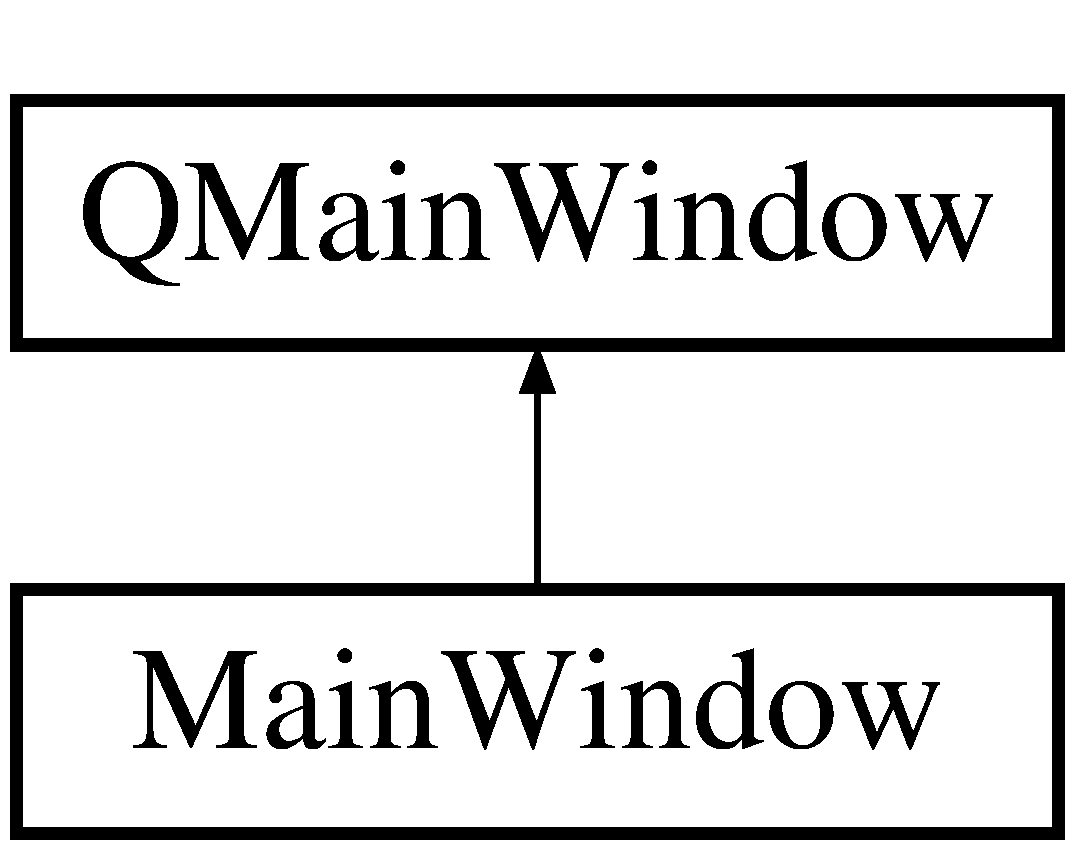
\includegraphics[height=2.000000cm]{class_main_window}
\end{center}
\end{figure}
\subsection*{Public Member Functions}
\begin{DoxyCompactItemize}
\item 
\hyperlink{class_main_window_a8b244be8b7b7db1b08de2a2acb9409db}{Main\+Window} (Q\+Widget $\ast$parent=0)
\item 
\hyperlink{class_main_window_ae98d00a93bc118200eeef9f9bba1dba7}{$\sim$\+Main\+Window} ()
\end{DoxyCompactItemize}


\subsection{Detailed Description}


Definition at line 6 of file mainwindow.\+h.



\subsection{Constructor \& Destructor Documentation}
\mbox{\Hypertarget{class_main_window_a8b244be8b7b7db1b08de2a2acb9409db}\label{class_main_window_a8b244be8b7b7db1b08de2a2acb9409db}} 
\index{Main\+Window@{Main\+Window}!Main\+Window@{Main\+Window}}
\index{Main\+Window@{Main\+Window}!Main\+Window@{Main\+Window}}
\subsubsection{\texorpdfstring{Main\+Window()}{MainWindow()}}
{\footnotesize\ttfamily Main\+Window\+::\+Main\+Window (\begin{DoxyParamCaption}\item[{Q\+Widget $\ast$}]{parent = {\ttfamily 0} }\end{DoxyParamCaption})}



Definition at line 3 of file mainwindow.\+cpp.


\begin{DoxyCode}
4     : QMainWindow(parent)
5 \{
6 \}
\end{DoxyCode}
\mbox{\Hypertarget{class_main_window_ae98d00a93bc118200eeef9f9bba1dba7}\label{class_main_window_ae98d00a93bc118200eeef9f9bba1dba7}} 
\index{Main\+Window@{Main\+Window}!````~Main\+Window@{$\sim$\+Main\+Window}}
\index{````~Main\+Window@{$\sim$\+Main\+Window}!Main\+Window@{Main\+Window}}
\subsubsection{\texorpdfstring{$\sim$\+Main\+Window()}{~MainWindow()}}
{\footnotesize\ttfamily Main\+Window\+::$\sim$\+Main\+Window (\begin{DoxyParamCaption}{ }\end{DoxyParamCaption})}



Definition at line 8 of file mainwindow.\+cpp.


\begin{DoxyCode}
9 \{
10 
11 \}
\end{DoxyCode}


The documentation for this class was generated from the following files\+:\begin{DoxyCompactItemize}
\item 
C\+:/\+Users/\+Fu\+Zzy/\+Dropbox/3de Jaar/\+Sem 1/\+R\+E\+I\+I313-\/\+C++ O\+O\+P/\+T\+D\+\_\+\+Game/\+Element\+\_\+\+T\+D/\hyperlink{mainwindow_8h}{mainwindow.\+h}\item 
C\+:/\+Users/\+Fu\+Zzy/\+Dropbox/3de Jaar/\+Sem 1/\+R\+E\+I\+I313-\/\+C++ O\+O\+P/\+T\+D\+\_\+\+Game/\+Element\+\_\+\+T\+D/\hyperlink{mainwindow_8cpp}{mainwindow.\+cpp}\end{DoxyCompactItemize}

\hypertarget{class_map}{}\section{Map Class Reference}
\label{class_map}\index{Map@{Map}}


{\ttfamily \#include $<$map.\+h$>$}

Inheritance diagram for Map\+:\begin{figure}[H]
\begin{center}
\leavevmode
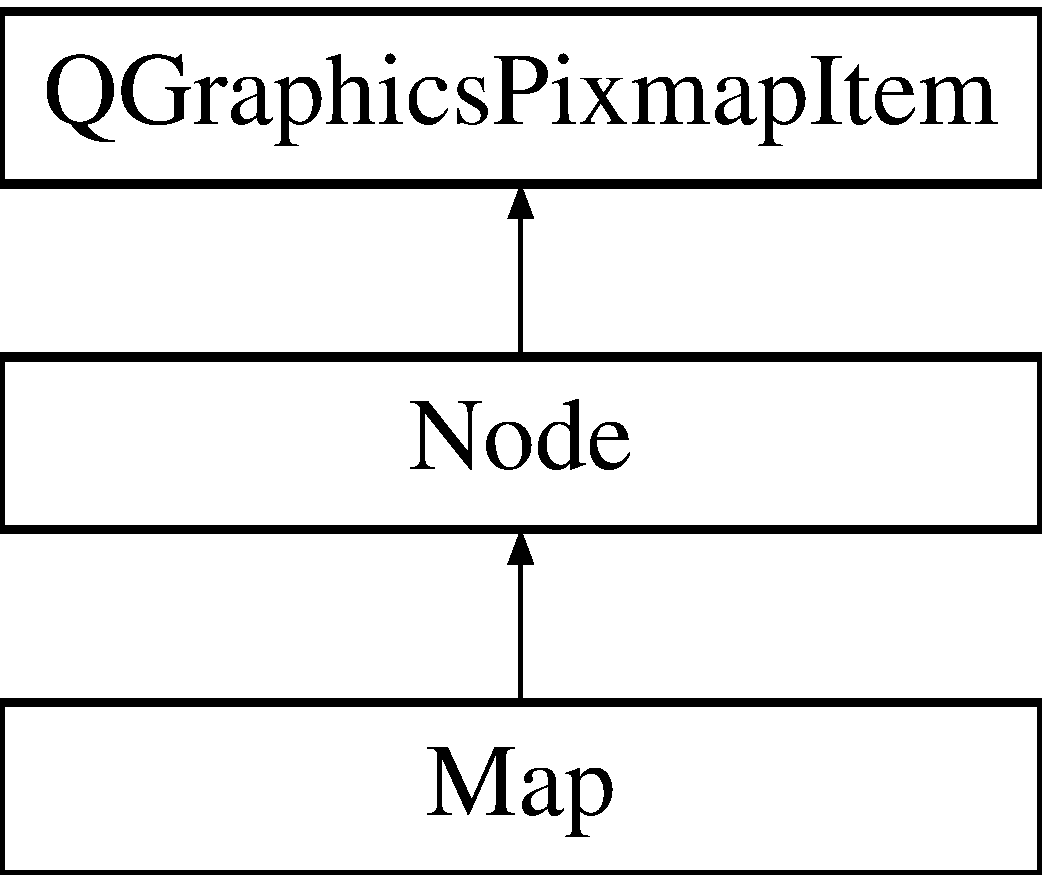
\includegraphics[height=3.000000cm]{class_map}
\end{center}
\end{figure}
\subsection*{Public Member Functions}
\begin{DoxyCompactItemize}
\item 
\hyperlink{class_map_a0f5ad0fd4563497b4214038cbca8b582}{Map} ()
\item 
int \hyperlink{class_map_a0c1055f7616a6779a7f5f1d561a8ccb2}{calcH} (\hyperlink{class_node}{Node} $\ast$a, \hyperlink{class_node}{Node} $\ast$b)
\item 
\hyperlink{class_node}{Node} $\ast$ \hyperlink{class_map_a19461c64e6da374e8022d210a6930867}{smallestF} ()
\item 
void \hyperlink{class_map_adac9fc32a2c840b40e1417292e846fe2}{calc\+Neighbours} (\hyperlink{class_node}{Node} $\ast$n)
\item 
\hyperlink{class_node}{Node} $\ast$ \hyperlink{class_map_a9500f43b02ce38b5e89248bd6e257858}{get\+Node} (int \hyperlink{class_node_aff1029a518bdc2651007b8856f958364}{x}, int \hyperlink{class_node_aa3e5b5240023b4528ae85057b3324202}{y})
\end{DoxyCompactItemize}
\subsection*{Public Attributes}
\begin{DoxyCompactItemize}
\item 
Q\+List$<$ Q\+PointF $>$ \hyperlink{class_map_a07f51de84c133707fedaeffd04aff2d5}{nodepoints}
\item 
\hyperlink{class_node}{Node} $\ast$ \hyperlink{class_map_a7298e7a7b5dbdc642c49ded9a2c754a5}{map} \mbox{[}\hyperlink{class_map_acfd20721da29a2e353598555e23e12f0}{mapX}\mbox{]}\mbox{[}\hyperlink{class_map_ae08efae9ac1453b2690985c627aca358}{mapY}\mbox{]}
\item 
Q\+Pixmap $\ast$ \hyperlink{class_map_af0167137084000cfb58a33df8474bcbe}{obstruction}
\item 
Q\+Pixmap $\ast$ \hyperlink{class_map_a99d78bd384bf091660dbc6e1123419b0}{path}
\item 
Q\+Pixmap $\ast$ \hyperlink{class_map_a322ef8e3f55269ef565a58f20190d148}{grass}
\item 
Q\+Pixmap $\ast$ \hyperlink{class_map_a4dafaf125d6014a97e98168e41492cd5}{portal}
\item 
\hyperlink{class_node}{Node} $\ast$ \hyperlink{class_map_aafcbf6f458eb48f4945f3d0b58d2ef85}{start}
\item 
\hyperlink{class_node}{Node} $\ast$ \hyperlink{class_map_abdb357cb53c27be3b6e3c2b54bfde669}{finish}
\item 
Q\+List$<$ \hyperlink{class_node}{Node} $\ast$ $>$ \hyperlink{class_map_ab19ca30427e7257d713f5fcfa0ac1a10}{open\+List}
\item 
Q\+List$<$ \hyperlink{class_node}{Node} $\ast$ $>$ \hyperlink{class_map_ae1ced58b787598940bb444659bacd7d3}{closed\+List}
\end{DoxyCompactItemize}
\subsection*{Static Public Attributes}
\begin{DoxyCompactItemize}
\item 
static const int \hyperlink{class_map_acfd20721da29a2e353598555e23e12f0}{mapX} = 11
\item 
static const int \hyperlink{class_map_ae08efae9ac1453b2690985c627aca358}{mapY} = 14
\item 
static const int \hyperlink{class_map_af2aa425dd22aba483ae973c4a15fe934}{tileX} = 64
\item 
static const int \hyperlink{class_map_a483dfba507cee9d2fa60a074992b1fcf}{tileY} = 64
\end{DoxyCompactItemize}


\subsection{Detailed Description}


Definition at line 9 of file map.\+h.



\subsection{Constructor \& Destructor Documentation}
\mbox{\Hypertarget{class_map_a0f5ad0fd4563497b4214038cbca8b582}\label{class_map_a0f5ad0fd4563497b4214038cbca8b582}} 
\index{Map@{Map}!Map@{Map}}
\index{Map@{Map}!Map@{Map}}
\subsubsection{\texorpdfstring{Map()}{Map()}}
{\footnotesize\ttfamily Map\+::\+Map (\begin{DoxyParamCaption}{ }\end{DoxyParamCaption})}



Definition at line 12 of file map.\+cpp.


\begin{DoxyCode}
13 \{
14     \textcolor{comment}{//initialize tiles}
15     \hyperlink{class_map_a322ef8e3f55269ef565a58f20190d148}{grass} = \textcolor{keyword}{new} QPixmap(\textcolor{stringliteral}{":/images/images/grass.png"});
16     \hyperlink{class_map_a99d78bd384bf091660dbc6e1123419b0}{path} = \textcolor{keyword}{new} QPixmap(\textcolor{stringliteral}{":/images/images/path.png"});
17     \hyperlink{class_map_af0167137084000cfb58a33df8474bcbe}{obstruction} = \textcolor{keyword}{new} QPixmap(\textcolor{stringliteral}{":/images/images/obstruction.png"});
18     \hyperlink{class_map_a4dafaf125d6014a97e98168e41492cd5}{portal} = \textcolor{keyword}{new} QPixmap(\textcolor{stringliteral}{":/images/images/portal.png"});
19 
20     \textcolor{comment}{//populate map}
21     \textcolor{comment}{//cout << "Start: " << clock() << " "  << endl;}
22     \textcolor{keywordflow}{for} (\textcolor{keywordtype}{int} \hyperlink{class_node_aff1029a518bdc2651007b8856f958364}{x}  = 0; \hyperlink{class_node_aff1029a518bdc2651007b8856f958364}{x} < \hyperlink{class_map_acfd20721da29a2e353598555e23e12f0}{mapX}; ++\hyperlink{class_node_aff1029a518bdc2651007b8856f958364}{x}) \{
23         \textcolor{keywordflow}{for} (\textcolor{keywordtype}{int} \hyperlink{class_node_aa3e5b5240023b4528ae85057b3324202}{y} = 0; \hyperlink{class_node_aa3e5b5240023b4528ae85057b3324202}{y} < \hyperlink{class_map_ae08efae9ac1453b2690985c627aca358}{mapY}; ++\hyperlink{class_node_aa3e5b5240023b4528ae85057b3324202}{y}) \{
24             \hyperlink{class_node}{Node} *t = \textcolor{keyword}{new} \hyperlink{class_node_a99ae3b67742635b847aff323ddd29b62}{Node};
25             t->\hyperlink{class_node_aae24f318bd4b6d14270084cec3fc98b5}{cost} = 1;
26             t->\hyperlink{class_node_aff1029a518bdc2651007b8856f958364}{x} = \hyperlink{class_node_aff1029a518bdc2651007b8856f958364}{x};
27             t->\hyperlink{class_node_aa3e5b5240023b4528ae85057b3324202}{y} = \hyperlink{class_node_aa3e5b5240023b4528ae85057b3324202}{y};
28             t->\hyperlink{class_node_a32fbe9e0f4fc9e9d1845ce808738d7ab}{f} = 0;
29             t->\hyperlink{class_node_a0b249888eacdec6c623ec8c58b230c48}{g} = 0;
30             t->\hyperlink{class_node_afb5a7ac7536a9e09488bb685420cd78a}{h} = 0;
31             t->\hyperlink{class_node_ad8184598cdea70e4bbdfd76f2b0f9e85}{parent} = 0;
32             t->\hyperlink{class_node_a2bb1959485873369ea2504c1dece3f33}{path} = \textcolor{keyword}{false};
33             t->\hyperlink{class_node_a2250e2c1710fb19f15f236ac69563613}{tile} = \hyperlink{node_8h_ac9e486ec80ccfdb28a4f4837d419c9f1a283b79b5e51a79e202e0702f189485ad}{Grass};
34             \textcolor{keywordtype}{int} x\_pos = \hyperlink{class_node_aff1029a518bdc2651007b8856f958364}{x}*pixmap().width() + pixmap().width()/2;
35             \textcolor{keywordtype}{int} y\_pos = \hyperlink{class_node_aa3e5b5240023b4528ae85057b3324202}{y}*pixmap().height() + pixmap().height()/2;
36             t->\hyperlink{class_node_a77faa088c74e20a361a181b58e8a4c7f}{point} = QPointF(x\_pos,y\_pos);
37             \hyperlink{class_map_a7298e7a7b5dbdc642c49ded9a2c754a5}{map}[\hyperlink{class_node_aff1029a518bdc2651007b8856f958364}{x}][\hyperlink{class_node_aa3e5b5240023b4528ae85057b3324202}{y}] = t;
38             \hyperlink{class_map_a7298e7a7b5dbdc642c49ded9a2c754a5}{map}[\hyperlink{class_node_aff1029a518bdc2651007b8856f958364}{x}][\hyperlink{class_node_aa3e5b5240023b4528ae85057b3324202}{y}]->setPos(\hyperlink{class_node_aff1029a518bdc2651007b8856f958364}{x},\hyperlink{class_node_aa3e5b5240023b4528ae85057b3324202}{y});
39             \hyperlink{class_map_a07f51de84c133707fedaeffd04aff2d5}{nodepoints} << QPointF(x\_pos, y\_pos);
40 
41         \}
42     \}
43 
44     \textcolor{comment}{//EDGES //add die cost}
45     \textcolor{comment}{/*top row*/}
46     \textcolor{keywordflow}{for} (\textcolor{keywordtype}{int} \hyperlink{class_node_aff1029a518bdc2651007b8856f958364}{x}  = 0; \hyperlink{class_node_aff1029a518bdc2651007b8856f958364}{x} < \hyperlink{class_map_acfd20721da29a2e353598555e23e12f0}{mapX}; ++\hyperlink{class_node_aff1029a518bdc2651007b8856f958364}{x}) \{
47         \textcolor{keywordflow}{for} (\textcolor{keywordtype}{int} \hyperlink{class_node_aa3e5b5240023b4528ae85057b3324202}{y} = 0; \hyperlink{class_node_aa3e5b5240023b4528ae85057b3324202}{y} < 1; ++\hyperlink{class_node_aa3e5b5240023b4528ae85057b3324202}{y}) \{
48             \hyperlink{class_node}{Node} *t = \textcolor{keyword}{new} \hyperlink{class_node_a99ae3b67742635b847aff323ddd29b62}{Node};
49             t->\hyperlink{class_node_a2250e2c1710fb19f15f236ac69563613}{tile} = \hyperlink{node_8h_ac9e486ec80ccfdb28a4f4837d419c9f1ae4afc87ae4a7816fdef8d05002e6dce4}{Obstruction};
50             t->\hyperlink{class_node_aae24f318bd4b6d14270084cec3fc98b5}{cost} = 100;
51             \hyperlink{class_map_a7298e7a7b5dbdc642c49ded9a2c754a5}{map}[\hyperlink{class_node_aff1029a518bdc2651007b8856f958364}{x}][\hyperlink{class_node_aa3e5b5240023b4528ae85057b3324202}{y}] = t;
52             t->setPixmap(QPixmap(\textcolor{stringliteral}{":/images/images/mapTile\_007.png"}));
53         \}
54     \}
55     \textcolor{comment}{/*bottom row*/}
56     \textcolor{keywordflow}{for} (\textcolor{keywordtype}{int} \hyperlink{class_node_aff1029a518bdc2651007b8856f958364}{x}  = 0; \hyperlink{class_node_aff1029a518bdc2651007b8856f958364}{x} < \hyperlink{class_map_acfd20721da29a2e353598555e23e12f0}{mapX}; ++\hyperlink{class_node_aff1029a518bdc2651007b8856f958364}{x}) \{
57         \textcolor{keywordflow}{for} (\textcolor{keywordtype}{int} \hyperlink{class_node_aa3e5b5240023b4528ae85057b3324202}{y} = mapY-1; \hyperlink{class_node_aa3e5b5240023b4528ae85057b3324202}{y} < \hyperlink{class_map_ae08efae9ac1453b2690985c627aca358}{mapY}; ++\hyperlink{class_node_aa3e5b5240023b4528ae85057b3324202}{y}) \{
58             \hyperlink{class_node}{Node} *t = \textcolor{keyword}{new} \hyperlink{class_node_a99ae3b67742635b847aff323ddd29b62}{Node};
59             t->\hyperlink{class_node_a2250e2c1710fb19f15f236ac69563613}{tile} = \hyperlink{node_8h_ac9e486ec80ccfdb28a4f4837d419c9f1ae4afc87ae4a7816fdef8d05002e6dce4}{Obstruction};
60             t->\hyperlink{class_node_aae24f318bd4b6d14270084cec3fc98b5}{cost} = 100;
61             \hyperlink{class_map_a7298e7a7b5dbdc642c49ded9a2c754a5}{map}[\hyperlink{class_node_aff1029a518bdc2651007b8856f958364}{x}][\hyperlink{class_node_aa3e5b5240023b4528ae85057b3324202}{y}] = t;
62             t->setPixmap(QPixmap(\textcolor{stringliteral}{":/images/images/mapTile\_052.png"}));
63         \}
64     \}
65 
66     \textcolor{comment}{/*left coloum*/}
67     \textcolor{keywordflow}{for} (\textcolor{keywordtype}{int} \hyperlink{class_node_aff1029a518bdc2651007b8856f958364}{x}  = 0; \hyperlink{class_node_aff1029a518bdc2651007b8856f958364}{x} < 1; ++\hyperlink{class_node_aff1029a518bdc2651007b8856f958364}{x}) \{
68         \textcolor{keywordflow}{for} (\textcolor{keywordtype}{int} \hyperlink{class_node_aa3e5b5240023b4528ae85057b3324202}{y} = 0; \hyperlink{class_node_aa3e5b5240023b4528ae85057b3324202}{y} < \hyperlink{class_map_ae08efae9ac1453b2690985c627aca358}{mapY}; ++\hyperlink{class_node_aa3e5b5240023b4528ae85057b3324202}{y}) \{
69             \hyperlink{class_node}{Node} *t = \textcolor{keyword}{new} \hyperlink{class_node_a99ae3b67742635b847aff323ddd29b62}{Node};
70             t->\hyperlink{class_node_a2250e2c1710fb19f15f236ac69563613}{tile} = \hyperlink{node_8h_ac9e486ec80ccfdb28a4f4837d419c9f1ae4afc87ae4a7816fdef8d05002e6dce4}{Obstruction};
71             t->\hyperlink{class_node_aae24f318bd4b6d14270084cec3fc98b5}{cost} = 100;
72             \hyperlink{class_map_a7298e7a7b5dbdc642c49ded9a2c754a5}{map}[\hyperlink{class_node_aff1029a518bdc2651007b8856f958364}{x}][\hyperlink{class_node_aa3e5b5240023b4528ae85057b3324202}{y}] = t;
73             t->setPixmap(QPixmap(\textcolor{stringliteral}{":/images/images/mapTile\_021.png"}));
74         \}
75     \}
76 
77     \textcolor{comment}{/*right coloum*/}
78     \textcolor{keywordflow}{for} (\textcolor{keywordtype}{int} \hyperlink{class_node_aff1029a518bdc2651007b8856f958364}{x}  = mapX-1; \hyperlink{class_node_aff1029a518bdc2651007b8856f958364}{x} < \hyperlink{class_map_acfd20721da29a2e353598555e23e12f0}{mapX}; ++\hyperlink{class_node_aff1029a518bdc2651007b8856f958364}{x}) \{
79         \textcolor{keywordflow}{for} (\textcolor{keywordtype}{int} \hyperlink{class_node_aa3e5b5240023b4528ae85057b3324202}{y} = 0; \hyperlink{class_node_aa3e5b5240023b4528ae85057b3324202}{y} < \hyperlink{class_map_ae08efae9ac1453b2690985c627aca358}{mapY}; ++\hyperlink{class_node_aa3e5b5240023b4528ae85057b3324202}{y}) \{
80             \hyperlink{class_node}{Node} *t = \textcolor{keyword}{new} \hyperlink{class_node_a99ae3b67742635b847aff323ddd29b62}{Node};
81             t->\hyperlink{class_node_a2250e2c1710fb19f15f236ac69563613}{tile} = \hyperlink{node_8h_ac9e486ec80ccfdb28a4f4837d419c9f1ae4afc87ae4a7816fdef8d05002e6dce4}{Obstruction};
82             t->\hyperlink{class_node_aae24f318bd4b6d14270084cec3fc98b5}{cost} = 100;
83             \hyperlink{class_map_a7298e7a7b5dbdc642c49ded9a2c754a5}{map}[\hyperlink{class_node_aff1029a518bdc2651007b8856f958364}{x}][\hyperlink{class_node_aa3e5b5240023b4528ae85057b3324202}{y}] = t;
84             t->setPixmap(QPixmap(\textcolor{stringliteral}{":/images/images/mapTile\_023.png"}));
85         \}
86     \}
87 
88 
89 
90     \textcolor{comment}{//portals}
91     \textcolor{comment}{/*Top portal*/}
92     \textcolor{keywordflow}{for} (\textcolor{keywordtype}{int} \hyperlink{class_node_aff1029a518bdc2651007b8856f958364}{x}  = mapX/2; \hyperlink{class_node_aff1029a518bdc2651007b8856f958364}{x} < mapX/2+1; ++\hyperlink{class_node_aff1029a518bdc2651007b8856f958364}{x}) \{
93         \textcolor{keywordflow}{for} (\textcolor{keywordtype}{int} \hyperlink{class_node_aa3e5b5240023b4528ae85057b3324202}{y} = 0; \hyperlink{class_node_aa3e5b5240023b4528ae85057b3324202}{y} < 1; ++\hyperlink{class_node_aa3e5b5240023b4528ae85057b3324202}{y}) \{
94             \hyperlink{class_node}{Node} *t = \textcolor{keyword}{new} \hyperlink{class_node_a99ae3b67742635b847aff323ddd29b62}{Node};
95             t->\hyperlink{class_node_aae24f318bd4b6d14270084cec3fc98b5}{cost} = 1;
96             t->\hyperlink{class_node_aff1029a518bdc2651007b8856f958364}{x} = \hyperlink{class_node_aff1029a518bdc2651007b8856f958364}{x};
97             t->\hyperlink{class_node_aa3e5b5240023b4528ae85057b3324202}{y} = \hyperlink{class_node_aa3e5b5240023b4528ae85057b3324202}{y};
98             t->\hyperlink{class_node_a32fbe9e0f4fc9e9d1845ce808738d7ab}{f} = 0;
99             t->\hyperlink{class_node_a0b249888eacdec6c623ec8c58b230c48}{g} = 0;
100             t->\hyperlink{class_node_afb5a7ac7536a9e09488bb685420cd78a}{h} = 0;
101             t->\hyperlink{class_node_ad8184598cdea70e4bbdfd76f2b0f9e85}{parent} = 0;
102             t->\hyperlink{class_node_a2bb1959485873369ea2504c1dece3f33}{path} = \textcolor{keyword}{false};
103             t->\hyperlink{class_node_a2250e2c1710fb19f15f236ac69563613}{tile} = \hyperlink{node_8h_ac9e486ec80ccfdb28a4f4837d419c9f1a283b79b5e51a79e202e0702f189485ad}{Grass};
104             \hyperlink{class_map_a7298e7a7b5dbdc642c49ded9a2c754a5}{map}[\hyperlink{class_node_aff1029a518bdc2651007b8856f958364}{x}][\hyperlink{class_node_aa3e5b5240023b4528ae85057b3324202}{y}] = t;
105             t->setPixmap(QPixmap(\textcolor{stringliteral}{":/images/images/portal.png"}));
106         \}
107     \}
108 
109     \textcolor{comment}{/*Bottom portal*/}
110     \textcolor{keywordflow}{for} (\textcolor{keywordtype}{int} \hyperlink{class_node_aff1029a518bdc2651007b8856f958364}{x}  = mapX/2; \hyperlink{class_node_aff1029a518bdc2651007b8856f958364}{x} < mapX/2+1; ++\hyperlink{class_node_aff1029a518bdc2651007b8856f958364}{x}) \{
111         \textcolor{keywordflow}{for} (\textcolor{keywordtype}{int} \hyperlink{class_node_aa3e5b5240023b4528ae85057b3324202}{y} = mapY-1; \hyperlink{class_node_aa3e5b5240023b4528ae85057b3324202}{y} < \hyperlink{class_map_ae08efae9ac1453b2690985c627aca358}{mapY}; ++\hyperlink{class_node_aa3e5b5240023b4528ae85057b3324202}{y}) \{
112             \hyperlink{class_node}{Node} *t = \textcolor{keyword}{new} \hyperlink{class_node_a99ae3b67742635b847aff323ddd29b62}{Node};
113             t->\hyperlink{class_node_aae24f318bd4b6d14270084cec3fc98b5}{cost} = 1;
114             t->\hyperlink{class_node_aff1029a518bdc2651007b8856f958364}{x} = \hyperlink{class_node_aff1029a518bdc2651007b8856f958364}{x};
115             t->\hyperlink{class_node_aa3e5b5240023b4528ae85057b3324202}{y} = \hyperlink{class_node_aa3e5b5240023b4528ae85057b3324202}{y};
116             t->\hyperlink{class_node_a32fbe9e0f4fc9e9d1845ce808738d7ab}{f} = 0;
117             t->\hyperlink{class_node_a0b249888eacdec6c623ec8c58b230c48}{g} = 0;
118             t->\hyperlink{class_node_afb5a7ac7536a9e09488bb685420cd78a}{h} = 0;
119             t->\hyperlink{class_node_ad8184598cdea70e4bbdfd76f2b0f9e85}{parent} = 0;
120             t->\hyperlink{class_node_a2bb1959485873369ea2504c1dece3f33}{path} = \textcolor{keyword}{false};
121             t->\hyperlink{class_node_a2250e2c1710fb19f15f236ac69563613}{tile} = \hyperlink{node_8h_ac9e486ec80ccfdb28a4f4837d419c9f1a283b79b5e51a79e202e0702f189485ad}{Grass};
122             \hyperlink{class_map_a7298e7a7b5dbdc642c49ded9a2c754a5}{map}[\hyperlink{class_node_aff1029a518bdc2651007b8856f958364}{x}][\hyperlink{class_node_aa3e5b5240023b4528ae85057b3324202}{y}] = t;
123             t->setPixmap(QPixmap(\textcolor{stringliteral}{":/images/images/portal.png"}));
124         \}
125     \}
126 
127 
128     \textcolor{comment}{//set beginning and en points}
129     \hyperlink{class_map_aafcbf6f458eb48f4945f3d0b58d2ef85}{start} = \hyperlink{class_map_a7298e7a7b5dbdc642c49ded9a2c754a5}{map}[mapX/2][0];
130     \hyperlink{class_map_abdb357cb53c27be3b6e3c2b54bfde669}{finish} = \hyperlink{class_map_a7298e7a7b5dbdc642c49ded9a2c754a5}{map}[mapX/2][mapY-1];
131     \hyperlink{class_map_aafcbf6f458eb48f4945f3d0b58d2ef85}{start}->\hyperlink{class_node_a77faa088c74e20a361a181b58e8a4c7f}{point} = QPointF(mapX*\hyperlink{class_map_af2aa425dd22aba483ae973c4a15fe934}{tileX}/2, \hyperlink{class_map_a483dfba507cee9d2fa60a074992b1fcf}{tileY}/2);
132     \hyperlink{class_map_abdb357cb53c27be3b6e3c2b54bfde669}{finish}->\hyperlink{class_node_a77faa088c74e20a361a181b58e8a4c7f}{point} = QPointF(mapX*\hyperlink{class_map_af2aa425dd22aba483ae973c4a15fe934}{tileX}/2, mapY*\hyperlink{class_map_a483dfba507cee9d2fa60a074992b1fcf}{tileY} - 
      \hyperlink{class_map_a483dfba507cee9d2fa60a074992b1fcf}{tileY}/2);
133 
134     \textcolor{comment}{//sets start node to closed list and calculate neighbors}
135     \hyperlink{class_map_ae1ced58b787598940bb444659bacd7d3}{closedList}.append(\hyperlink{class_map_aafcbf6f458eb48f4945f3d0b58d2ef85}{start});
136     \hyperlink{class_map_adac9fc32a2c840b40e1417292e846fe2}{calcNeighbours}(\hyperlink{class_map_aafcbf6f458eb48f4945f3d0b58d2ef85}{start});
137 
138     \textcolor{comment}{//start A*}
139     \textcolor{comment}{//cout << "InitMap" << clock() << endl;}
140 
141 \textcolor{comment}{//    while (openList.length() > 0)}
142 \textcolor{comment}{//    \{}
143 \textcolor{comment}{//        Node *t = smallestF();}
144 \textcolor{comment}{//        closedList.append(t);}
145 \textcolor{comment}{//        if (t == finish)}
146 \textcolor{comment}{//        \{}
147 \textcolor{comment}{//            while (t->parent)}
148 \textcolor{comment}{//            \{}
149 \textcolor{comment}{//                t->path = true;}
150 \textcolor{comment}{//                t = t->parent;}
151 \textcolor{comment}{//                t->tile = Path;}
152 \textcolor{comment}{//                game->pointsToFollow << point;}
153 \textcolor{comment}{//            \}}
154 
155 \textcolor{comment}{//        \}}
156 \textcolor{comment}{//        calcNeighbours(t);}
157 \textcolor{comment}{//    \}}
158 
159     \textcolor{comment}{//cout << "Path found: " << clock() << endl;}
160 
161     \textcolor{comment}{//cout << " Map printed: " << clock() << endl;}
162 
163 
164 \}
\end{DoxyCode}


\subsection{Member Function Documentation}
\mbox{\Hypertarget{class_map_a0c1055f7616a6779a7f5f1d561a8ccb2}\label{class_map_a0c1055f7616a6779a7f5f1d561a8ccb2}} 
\index{Map@{Map}!calcH@{calcH}}
\index{calcH@{calcH}!Map@{Map}}
\subsubsection{\texorpdfstring{calc\+H()}{calcH()}}
{\footnotesize\ttfamily int Map\+::calcH (\begin{DoxyParamCaption}\item[{\hyperlink{class_node}{Node} $\ast$}]{a,  }\item[{\hyperlink{class_node}{Node} $\ast$}]{b }\end{DoxyParamCaption})}



Definition at line 166 of file map.\+cpp.


\begin{DoxyCode}
167 \{
168     \textcolor{keywordtype}{int} \hyperlink{class_node_aff1029a518bdc2651007b8856f958364}{x}, \hyperlink{class_node_aa3e5b5240023b4528ae85057b3324202}{y};
169     a->\hyperlink{class_node_aff1029a518bdc2651007b8856f958364}{x} - b->\hyperlink{class_node_aff1029a518bdc2651007b8856f958364}{x} >= 0 ? x = a->\hyperlink{class_node_aff1029a518bdc2651007b8856f958364}{x} - b->\hyperlink{class_node_aff1029a518bdc2651007b8856f958364}{x} : x = b->\hyperlink{class_node_aff1029a518bdc2651007b8856f958364}{x}; \textcolor{comment}{//weti of kla}
170     a->\hyperlink{class_node_aa3e5b5240023b4528ae85057b3324202}{y} - b->\hyperlink{class_node_aa3e5b5240023b4528ae85057b3324202}{y} >= 0 ? y = a->\hyperlink{class_node_aa3e5b5240023b4528ae85057b3324202}{y} - b->\hyperlink{class_node_aa3e5b5240023b4528ae85057b3324202}{y} : y = b->\hyperlink{class_node_aa3e5b5240023b4528ae85057b3324202}{y}; \textcolor{comment}{//weti of kla}
171     \textcolor{keywordflow}{return} x >= y ? x * 10 : y * 10;
172 \}
\end{DoxyCode}
\mbox{\Hypertarget{class_map_adac9fc32a2c840b40e1417292e846fe2}\label{class_map_adac9fc32a2c840b40e1417292e846fe2}} 
\index{Map@{Map}!calc\+Neighbours@{calc\+Neighbours}}
\index{calc\+Neighbours@{calc\+Neighbours}!Map@{Map}}
\subsubsection{\texorpdfstring{calc\+Neighbours()}{calcNeighbours()}}
{\footnotesize\ttfamily void Map\+::calc\+Neighbours (\begin{DoxyParamCaption}\item[{\hyperlink{class_node}{Node} $\ast$}]{n }\end{DoxyParamCaption})}



Definition at line 188 of file map.\+cpp.


\begin{DoxyCode}
189 \{
190     \textcolor{keywordflow}{for} (\textcolor{keywordtype}{int} dy = -1; dy <= 1; ++dy)
191     \{
192         \textcolor{keywordflow}{for} (\textcolor{keywordtype}{int} dx = -1; dx <= 1; ++dx)
193         \{
194             \textcolor{keywordtype}{int} \hyperlink{class_node_aff1029a518bdc2651007b8856f958364}{x} = dx + n->\hyperlink{class_node_aff1029a518bdc2651007b8856f958364}{x};
195             \textcolor{keywordtype}{int} \hyperlink{class_node_aa3e5b5240023b4528ae85057b3324202}{y} = dy + n->\hyperlink{class_node_aa3e5b5240023b4528ae85057b3324202}{y};
196             \textcolor{keywordflow}{if} ((x>=0) && (x < \hyperlink{class_map_acfd20721da29a2e353598555e23e12f0}{mapX}) && (y>=0) && (y < \hyperlink{class_map_ae08efae9ac1453b2690985c627aca358}{mapY}) &&
197                 (!\hyperlink{class_map_ab19ca30427e7257d713f5fcfa0ac1a10}{openList}.contains(\hyperlink{class_map_a7298e7a7b5dbdc642c49ded9a2c754a5}{map}[x][y])) && (!\hyperlink{class_map_ae1ced58b787598940bb444659bacd7d3}{closedList}.contains(
      \hyperlink{class_map_a7298e7a7b5dbdc642c49ded9a2c754a5}{map}[x][y])) &&
198                 (\hyperlink{class_map_a7298e7a7b5dbdc642c49ded9a2c754a5}{map}[x][y]->\hyperlink{class_node_aae24f318bd4b6d14270084cec3fc98b5}{cost} < 100) && ((dx*dx) || (dy*dy)) && ((dy*dy) != (dx*dx))) \textcolor{comment}{//haal
       laaste uit vir nei diag}
199             \{
200                 \hyperlink{class_map_a7298e7a7b5dbdc642c49ded9a2c754a5}{map}[\hyperlink{class_node_aff1029a518bdc2651007b8856f958364}{x}][\hyperlink{class_node_aa3e5b5240023b4528ae85057b3324202}{y}]->\hyperlink{class_node_ad8184598cdea70e4bbdfd76f2b0f9e85}{parent} = n;
201                 \textcolor{keywordflow}{if} ((dx*dx) && (dy*dy))
202                 \{
203                     \hyperlink{class_map_a7298e7a7b5dbdc642c49ded9a2c754a5}{map}[\hyperlink{class_node_aff1029a518bdc2651007b8856f958364}{x}][\hyperlink{class_node_aa3e5b5240023b4528ae85057b3324202}{y}]->\hyperlink{class_node_a0b249888eacdec6c623ec8c58b230c48}{g} = n->\hyperlink{class_node_a0b249888eacdec6c623ec8c58b230c48}{g} + 14;
204                 \}
205                 \textcolor{keywordflow}{else}
206                 \{
207                     \hyperlink{class_map_a7298e7a7b5dbdc642c49ded9a2c754a5}{map}[\hyperlink{class_node_aff1029a518bdc2651007b8856f958364}{x}][\hyperlink{class_node_aa3e5b5240023b4528ae85057b3324202}{y}]->\hyperlink{class_node_a0b249888eacdec6c623ec8c58b230c48}{g} = n->\hyperlink{class_node_a0b249888eacdec6c623ec8c58b230c48}{g} + 10;
208                 \}
209                 \hyperlink{class_map_a7298e7a7b5dbdc642c49ded9a2c754a5}{map}[\hyperlink{class_node_aff1029a518bdc2651007b8856f958364}{x}][\hyperlink{class_node_aa3e5b5240023b4528ae85057b3324202}{y}]->\hyperlink{class_node_afb5a7ac7536a9e09488bb685420cd78a}{h} = \hyperlink{class_map_a0c1055f7616a6779a7f5f1d561a8ccb2}{calcH}(\hyperlink{class_map_a7298e7a7b5dbdc642c49ded9a2c754a5}{map}[x][y], \hyperlink{class_map_abdb357cb53c27be3b6e3c2b54bfde669}{finish});
210                 \hyperlink{class_map_a7298e7a7b5dbdc642c49ded9a2c754a5}{map}[\hyperlink{class_node_aff1029a518bdc2651007b8856f958364}{x}][\hyperlink{class_node_aa3e5b5240023b4528ae85057b3324202}{y}]->\hyperlink{class_node_a32fbe9e0f4fc9e9d1845ce808738d7ab}{f} = \hyperlink{class_map_a7298e7a7b5dbdc642c49ded9a2c754a5}{map}[\hyperlink{class_node_aff1029a518bdc2651007b8856f958364}{x}][\hyperlink{class_node_aa3e5b5240023b4528ae85057b3324202}{y}]->\hyperlink{class_node_a0b249888eacdec6c623ec8c58b230c48}{g} + \hyperlink{class_map_a7298e7a7b5dbdc642c49ded9a2c754a5}{map}[\hyperlink{class_node_aff1029a518bdc2651007b8856f958364}{x}][\hyperlink{class_node_aa3e5b5240023b4528ae85057b3324202}{y}]->\hyperlink{class_node_afb5a7ac7536a9e09488bb685420cd78a}{h};
211                 \hyperlink{class_map_ab19ca30427e7257d713f5fcfa0ac1a10}{openList}.append(\hyperlink{class_map_a7298e7a7b5dbdc642c49ded9a2c754a5}{map}[x][y]);
212             \}
213         \}
214     \}
215 \}
\end{DoxyCode}
\mbox{\Hypertarget{class_map_a9500f43b02ce38b5e89248bd6e257858}\label{class_map_a9500f43b02ce38b5e89248bd6e257858}} 
\index{Map@{Map}!get\+Node@{get\+Node}}
\index{get\+Node@{get\+Node}!Map@{Map}}
\subsubsection{\texorpdfstring{get\+Node()}{getNode()}}
{\footnotesize\ttfamily \hyperlink{class_node}{Node} $\ast$ Map\+::get\+Node (\begin{DoxyParamCaption}\item[{int}]{x,  }\item[{int}]{y }\end{DoxyParamCaption})}



Definition at line 217 of file map.\+cpp.


\begin{DoxyCode}
218 \{
219     \textcolor{keywordflow}{return} \hyperlink{class_map_a7298e7a7b5dbdc642c49ded9a2c754a5}{map}[\hyperlink{class_node_aff1029a518bdc2651007b8856f958364}{x}][\hyperlink{class_node_aa3e5b5240023b4528ae85057b3324202}{y}];
220 \}
\end{DoxyCode}
\mbox{\Hypertarget{class_map_a19461c64e6da374e8022d210a6930867}\label{class_map_a19461c64e6da374e8022d210a6930867}} 
\index{Map@{Map}!smallestF@{smallestF}}
\index{smallestF@{smallestF}!Map@{Map}}
\subsubsection{\texorpdfstring{smallest\+F()}{smallestF()}}
{\footnotesize\ttfamily \hyperlink{class_node}{Node} $\ast$ Map\+::smallestF (\begin{DoxyParamCaption}{ }\end{DoxyParamCaption})}



Definition at line 174 of file map.\+cpp.


\begin{DoxyCode}
175 \{
176     \hyperlink{class_node}{Node} *r = \hyperlink{class_map_ab19ca30427e7257d713f5fcfa0ac1a10}{openList}.first();
177     QListIterator<Node*> i(\hyperlink{class_map_ab19ca30427e7257d713f5fcfa0ac1a10}{openList});
178     \textcolor{keywordflow}{while} (i.hasNext())
179     \{
180         \hyperlink{class_node}{Node} *t = i.next();
181         \textcolor{keywordflow}{if} (t->\hyperlink{class_node_a32fbe9e0f4fc9e9d1845ce808738d7ab}{f} < r->\hyperlink{class_node_a32fbe9e0f4fc9e9d1845ce808738d7ab}{f})
182             r = t;
183     \}
184     \hyperlink{class_map_ab19ca30427e7257d713f5fcfa0ac1a10}{openList}.removeOne(r);
185     \textcolor{keywordflow}{return} r;
186 \}
\end{DoxyCode}


\subsection{Member Data Documentation}
\mbox{\Hypertarget{class_map_ae1ced58b787598940bb444659bacd7d3}\label{class_map_ae1ced58b787598940bb444659bacd7d3}} 
\index{Map@{Map}!closed\+List@{closed\+List}}
\index{closed\+List@{closed\+List}!Map@{Map}}
\subsubsection{\texorpdfstring{closed\+List}{closedList}}
{\footnotesize\ttfamily Q\+List$<$\hyperlink{class_node}{Node}$\ast$$>$ Map\+::closed\+List}



Definition at line 30 of file map.\+h.

\mbox{\Hypertarget{class_map_abdb357cb53c27be3b6e3c2b54bfde669}\label{class_map_abdb357cb53c27be3b6e3c2b54bfde669}} 
\index{Map@{Map}!finish@{finish}}
\index{finish@{finish}!Map@{Map}}
\subsubsection{\texorpdfstring{finish}{finish}}
{\footnotesize\ttfamily \hyperlink{class_node}{Node}$\ast$ Map\+::finish}



Definition at line 28 of file map.\+h.

\mbox{\Hypertarget{class_map_a322ef8e3f55269ef565a58f20190d148}\label{class_map_a322ef8e3f55269ef565a58f20190d148}} 
\index{Map@{Map}!grass@{grass}}
\index{grass@{grass}!Map@{Map}}
\subsubsection{\texorpdfstring{grass}{grass}}
{\footnotesize\ttfamily Q\+Pixmap $\ast$ Map\+::grass}



Definition at line 26 of file map.\+h.

\mbox{\Hypertarget{class_map_a7298e7a7b5dbdc642c49ded9a2c754a5}\label{class_map_a7298e7a7b5dbdc642c49ded9a2c754a5}} 
\index{Map@{Map}!map@{map}}
\index{map@{map}!Map@{Map}}
\subsubsection{\texorpdfstring{map}{map}}
{\footnotesize\ttfamily \hyperlink{class_node}{Node}$\ast$ Map\+::map\mbox{[}\hyperlink{class_map_acfd20721da29a2e353598555e23e12f0}{mapX}\mbox{]}\mbox{[}\hyperlink{class_map_ae08efae9ac1453b2690985c627aca358}{mapY}\mbox{]}}



Definition at line 25 of file map.\+h.

\mbox{\Hypertarget{class_map_acfd20721da29a2e353598555e23e12f0}\label{class_map_acfd20721da29a2e353598555e23e12f0}} 
\index{Map@{Map}!mapX@{mapX}}
\index{mapX@{mapX}!Map@{Map}}
\subsubsection{\texorpdfstring{mapX}{mapX}}
{\footnotesize\ttfamily const int Map\+::mapX = 11\hspace{0.3cm}{\ttfamily [static]}}



Definition at line 21 of file map.\+h.

\mbox{\Hypertarget{class_map_ae08efae9ac1453b2690985c627aca358}\label{class_map_ae08efae9ac1453b2690985c627aca358}} 
\index{Map@{Map}!mapY@{mapY}}
\index{mapY@{mapY}!Map@{Map}}
\subsubsection{\texorpdfstring{mapY}{mapY}}
{\footnotesize\ttfamily const int Map\+::mapY = 14\hspace{0.3cm}{\ttfamily [static]}}



Definition at line 22 of file map.\+h.

\mbox{\Hypertarget{class_map_a07f51de84c133707fedaeffd04aff2d5}\label{class_map_a07f51de84c133707fedaeffd04aff2d5}} 
\index{Map@{Map}!nodepoints@{nodepoints}}
\index{nodepoints@{nodepoints}!Map@{Map}}
\subsubsection{\texorpdfstring{nodepoints}{nodepoints}}
{\footnotesize\ttfamily Q\+List$<$Q\+PointF$>$ Map\+::nodepoints}



Definition at line 19 of file map.\+h.

\mbox{\Hypertarget{class_map_af0167137084000cfb58a33df8474bcbe}\label{class_map_af0167137084000cfb58a33df8474bcbe}} 
\index{Map@{Map}!obstruction@{obstruction}}
\index{obstruction@{obstruction}!Map@{Map}}
\subsubsection{\texorpdfstring{obstruction}{obstruction}}
{\footnotesize\ttfamily Q\+Pixmap$\ast$ Map\+::obstruction}



Definition at line 26 of file map.\+h.

\mbox{\Hypertarget{class_map_ab19ca30427e7257d713f5fcfa0ac1a10}\label{class_map_ab19ca30427e7257d713f5fcfa0ac1a10}} 
\index{Map@{Map}!open\+List@{open\+List}}
\index{open\+List@{open\+List}!Map@{Map}}
\subsubsection{\texorpdfstring{open\+List}{openList}}
{\footnotesize\ttfamily Q\+List$<$\hyperlink{class_node}{Node}$\ast$$>$ Map\+::open\+List}



Definition at line 29 of file map.\+h.

\mbox{\Hypertarget{class_map_a99d78bd384bf091660dbc6e1123419b0}\label{class_map_a99d78bd384bf091660dbc6e1123419b0}} 
\index{Map@{Map}!path@{path}}
\index{path@{path}!Map@{Map}}
\subsubsection{\texorpdfstring{path}{path}}
{\footnotesize\ttfamily Q\+Pixmap $\ast$ Map\+::path}



Definition at line 26 of file map.\+h.

\mbox{\Hypertarget{class_map_a4dafaf125d6014a97e98168e41492cd5}\label{class_map_a4dafaf125d6014a97e98168e41492cd5}} 
\index{Map@{Map}!portal@{portal}}
\index{portal@{portal}!Map@{Map}}
\subsubsection{\texorpdfstring{portal}{portal}}
{\footnotesize\ttfamily Q\+Pixmap $\ast$ Map\+::portal}



Definition at line 26 of file map.\+h.

\mbox{\Hypertarget{class_map_aafcbf6f458eb48f4945f3d0b58d2ef85}\label{class_map_aafcbf6f458eb48f4945f3d0b58d2ef85}} 
\index{Map@{Map}!start@{start}}
\index{start@{start}!Map@{Map}}
\subsubsection{\texorpdfstring{start}{start}}
{\footnotesize\ttfamily \hyperlink{class_node}{Node}$\ast$ Map\+::start}



Definition at line 27 of file map.\+h.

\mbox{\Hypertarget{class_map_af2aa425dd22aba483ae973c4a15fe934}\label{class_map_af2aa425dd22aba483ae973c4a15fe934}} 
\index{Map@{Map}!tileX@{tileX}}
\index{tileX@{tileX}!Map@{Map}}
\subsubsection{\texorpdfstring{tileX}{tileX}}
{\footnotesize\ttfamily const int Map\+::tileX = 64\hspace{0.3cm}{\ttfamily [static]}}



Definition at line 23 of file map.\+h.

\mbox{\Hypertarget{class_map_a483dfba507cee9d2fa60a074992b1fcf}\label{class_map_a483dfba507cee9d2fa60a074992b1fcf}} 
\index{Map@{Map}!tileY@{tileY}}
\index{tileY@{tileY}!Map@{Map}}
\subsubsection{\texorpdfstring{tileY}{tileY}}
{\footnotesize\ttfamily const int Map\+::tileY = 64\hspace{0.3cm}{\ttfamily [static]}}



Definition at line 24 of file map.\+h.



The documentation for this class was generated from the following files\+:\begin{DoxyCompactItemize}
\item 
C\+:/\+Users/\+Fu\+Zzy/\+Dropbox/3de Jaar/\+Sem 1/\+R\+E\+I\+I313-\/\+C++ O\+O\+P/\+T\+D\+\_\+\+Game/\+Element\+\_\+\+T\+D/\hyperlink{map_8h}{map.\+h}\item 
C\+:/\+Users/\+Fu\+Zzy/\+Dropbox/3de Jaar/\+Sem 1/\+R\+E\+I\+I313-\/\+C++ O\+O\+P/\+T\+D\+\_\+\+Game/\+Element\+\_\+\+T\+D/\hyperlink{map_8cpp}{map.\+cpp}\end{DoxyCompactItemize}

\hypertarget{class_node}{}\section{Node Class Reference}
\label{class_node}\index{Node@{Node}}


{\ttfamily \#include $<$node.\+h$>$}

Inheritance diagram for Node\+:\begin{figure}[H]
\begin{center}
\leavevmode
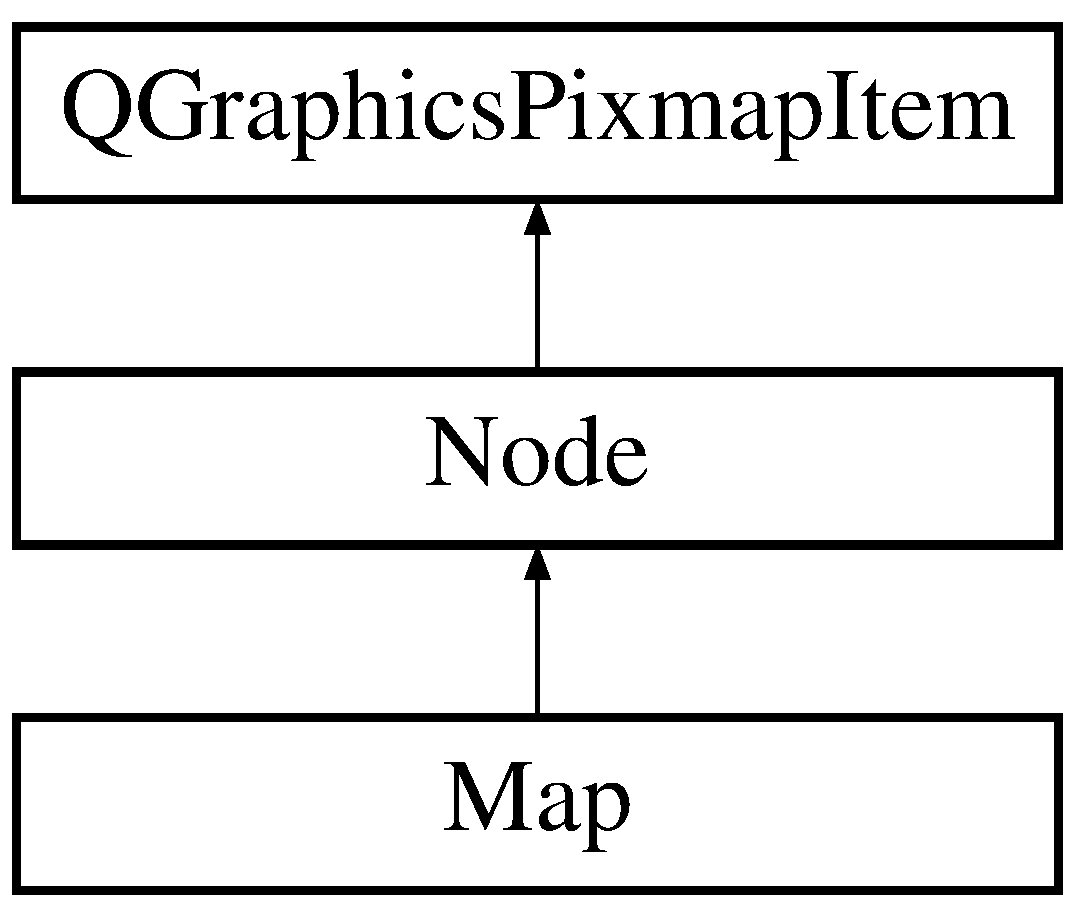
\includegraphics[height=3.000000cm]{class_node}
\end{center}
\end{figure}
\subsection*{Public Member Functions}
\begin{DoxyCompactItemize}
\item 
\hyperlink{class_node_a99ae3b67742635b847aff323ddd29b62}{Node} (Q\+Graphics\+Item $\ast$\hyperlink{class_node_ad8184598cdea70e4bbdfd76f2b0f9e85}{parent}=0)
\end{DoxyCompactItemize}
\subsection*{Public Attributes}
\begin{DoxyCompactItemize}
\item 
Q\+Label $\ast$ \hyperlink{class_node_a95d9b57b8efb3807c994314c3ff444b7}{label}
\item 
\hyperlink{node_8h_ac9e486ec80ccfdb28a4f4837d419c9f1}{Tile\+Type} \hyperlink{class_node_a2250e2c1710fb19f15f236ac69563613}{tile}
\item 
int \hyperlink{class_node_aae24f318bd4b6d14270084cec3fc98b5}{cost}
\item 
int \hyperlink{class_node_aff1029a518bdc2651007b8856f958364}{x}
\item 
int \hyperlink{class_node_aa3e5b5240023b4528ae85057b3324202}{y}
\item 
int \hyperlink{class_node_a32fbe9e0f4fc9e9d1845ce808738d7ab}{f}
\item 
int \hyperlink{class_node_a0b249888eacdec6c623ec8c58b230c48}{g}
\item 
int \hyperlink{class_node_afb5a7ac7536a9e09488bb685420cd78a}{h}
\item 
\hyperlink{class_node}{Node} $\ast$ \hyperlink{class_node_ad8184598cdea70e4bbdfd76f2b0f9e85}{parent}
\item 
bool \hyperlink{class_node_a2bb1959485873369ea2504c1dece3f33}{path}
\item 
Q\+PointF \hyperlink{class_node_a77faa088c74e20a361a181b58e8a4c7f}{point}
\end{DoxyCompactItemize}


\subsection{Detailed Description}


Definition at line 15 of file node.\+h.



\subsection{Constructor \& Destructor Documentation}
\mbox{\Hypertarget{class_node_a99ae3b67742635b847aff323ddd29b62}\label{class_node_a99ae3b67742635b847aff323ddd29b62}} 
\index{Node@{Node}!Node@{Node}}
\index{Node@{Node}!Node@{Node}}
\subsubsection{\texorpdfstring{Node()}{Node()}}
{\footnotesize\ttfamily Node\+::\+Node (\begin{DoxyParamCaption}\item[{Q\+Graphics\+Item $\ast$}]{parent = {\ttfamily 0} }\end{DoxyParamCaption})}



Definition at line 4 of file node.\+cpp.


\begin{DoxyCode}
5 \{
6     setPixmap(QPixmap(\textcolor{stringliteral}{":/images/images/grass.png"}));
7 \}
\end{DoxyCode}


\subsection{Member Data Documentation}
\mbox{\Hypertarget{class_node_aae24f318bd4b6d14270084cec3fc98b5}\label{class_node_aae24f318bd4b6d14270084cec3fc98b5}} 
\index{Node@{Node}!cost@{cost}}
\index{cost@{cost}!Node@{Node}}
\subsubsection{\texorpdfstring{cost}{cost}}
{\footnotesize\ttfamily int Node\+::cost}



Definition at line 21 of file node.\+h.

\mbox{\Hypertarget{class_node_a32fbe9e0f4fc9e9d1845ce808738d7ab}\label{class_node_a32fbe9e0f4fc9e9d1845ce808738d7ab}} 
\index{Node@{Node}!f@{f}}
\index{f@{f}!Node@{Node}}
\subsubsection{\texorpdfstring{f}{f}}
{\footnotesize\ttfamily int Node\+::f}



Definition at line 24 of file node.\+h.

\mbox{\Hypertarget{class_node_a0b249888eacdec6c623ec8c58b230c48}\label{class_node_a0b249888eacdec6c623ec8c58b230c48}} 
\index{Node@{Node}!g@{g}}
\index{g@{g}!Node@{Node}}
\subsubsection{\texorpdfstring{g}{g}}
{\footnotesize\ttfamily int Node\+::g}



Definition at line 25 of file node.\+h.

\mbox{\Hypertarget{class_node_afb5a7ac7536a9e09488bb685420cd78a}\label{class_node_afb5a7ac7536a9e09488bb685420cd78a}} 
\index{Node@{Node}!h@{h}}
\index{h@{h}!Node@{Node}}
\subsubsection{\texorpdfstring{h}{h}}
{\footnotesize\ttfamily int Node\+::h}



Definition at line 26 of file node.\+h.

\mbox{\Hypertarget{class_node_a95d9b57b8efb3807c994314c3ff444b7}\label{class_node_a95d9b57b8efb3807c994314c3ff444b7}} 
\index{Node@{Node}!label@{label}}
\index{label@{label}!Node@{Node}}
\subsubsection{\texorpdfstring{label}{label}}
{\footnotesize\ttfamily Q\+Label$\ast$ Node\+::label}



Definition at line 19 of file node.\+h.

\mbox{\Hypertarget{class_node_ad8184598cdea70e4bbdfd76f2b0f9e85}\label{class_node_ad8184598cdea70e4bbdfd76f2b0f9e85}} 
\index{Node@{Node}!parent@{parent}}
\index{parent@{parent}!Node@{Node}}
\subsubsection{\texorpdfstring{parent}{parent}}
{\footnotesize\ttfamily \hyperlink{class_node}{Node}$\ast$ Node\+::parent}



Definition at line 27 of file node.\+h.

\mbox{\Hypertarget{class_node_a2bb1959485873369ea2504c1dece3f33}\label{class_node_a2bb1959485873369ea2504c1dece3f33}} 
\index{Node@{Node}!path@{path}}
\index{path@{path}!Node@{Node}}
\subsubsection{\texorpdfstring{path}{path}}
{\footnotesize\ttfamily bool Node\+::path}



Definition at line 28 of file node.\+h.

\mbox{\Hypertarget{class_node_a77faa088c74e20a361a181b58e8a4c7f}\label{class_node_a77faa088c74e20a361a181b58e8a4c7f}} 
\index{Node@{Node}!point@{point}}
\index{point@{point}!Node@{Node}}
\subsubsection{\texorpdfstring{point}{point}}
{\footnotesize\ttfamily Q\+PointF Node\+::point}



Definition at line 29 of file node.\+h.

\mbox{\Hypertarget{class_node_a2250e2c1710fb19f15f236ac69563613}\label{class_node_a2250e2c1710fb19f15f236ac69563613}} 
\index{Node@{Node}!tile@{tile}}
\index{tile@{tile}!Node@{Node}}
\subsubsection{\texorpdfstring{tile}{tile}}
{\footnotesize\ttfamily \hyperlink{node_8h_ac9e486ec80ccfdb28a4f4837d419c9f1}{Tile\+Type} Node\+::tile}



Definition at line 20 of file node.\+h.

\mbox{\Hypertarget{class_node_aff1029a518bdc2651007b8856f958364}\label{class_node_aff1029a518bdc2651007b8856f958364}} 
\index{Node@{Node}!x@{x}}
\index{x@{x}!Node@{Node}}
\subsubsection{\texorpdfstring{x}{x}}
{\footnotesize\ttfamily int Node\+::x}



Definition at line 22 of file node.\+h.

\mbox{\Hypertarget{class_node_aa3e5b5240023b4528ae85057b3324202}\label{class_node_aa3e5b5240023b4528ae85057b3324202}} 
\index{Node@{Node}!y@{y}}
\index{y@{y}!Node@{Node}}
\subsubsection{\texorpdfstring{y}{y}}
{\footnotesize\ttfamily int Node\+::y}



Definition at line 23 of file node.\+h.



The documentation for this class was generated from the following files\+:\begin{DoxyCompactItemize}
\item 
C\+:/\+Users/\+Fu\+Zzy/\+Dropbox/3de Jaar/\+Sem 1/\+R\+E\+I\+I313-\/\+C++ O\+O\+P/\+T\+D\+\_\+\+Game/\+Element\+\_\+\+T\+D/\hyperlink{node_8h}{node.\+h}\item 
C\+:/\+Users/\+Fu\+Zzy/\+Dropbox/3de Jaar/\+Sem 1/\+R\+E\+I\+I313-\/\+C++ O\+O\+P/\+T\+D\+\_\+\+Game/\+Element\+\_\+\+T\+D/\hyperlink{node_8cpp}{node.\+cpp}\end{DoxyCompactItemize}

\hypertarget{class_player1}{}\section{Player1 Class Reference}
\label{class_player1}\index{Player1@{Player1}}


{\ttfamily \#include $<$player1.\+h$>$}

\subsection*{Public Member Functions}
\begin{DoxyCompactItemize}
\item 
\hyperlink{class_player1_a412188402865939ebc4e2aa1e5a214a2}{Player1} ()
\item 
int \hyperlink{class_player1_a9395a16fecb7b96395455f096ac1b60b}{get\+Gold} ()
\item 
int \hyperlink{class_player1_afb2adc7bd83c6380fbb85a832e083f4d}{get\+Lives} ()
\item 
int \hyperlink{class_player1_a1bc2927827b94667b6f2d115ae95fb75}{get\+Income} ()
\item 
void \hyperlink{class_player1_afb8807754032eba459edf031bb344653}{set\+Gold} (int gold)
\item 
void \hyperlink{class_player1_ac12457900903d22789531287e9934b8b}{set\+Lives} (int lives)
\item 
void \hyperlink{class_player1_a2e44127463fa785a00a0e118d5e8cf4f}{set\+Income} (int income)
\end{DoxyCompactItemize}
\subsection*{Public Attributes}
\begin{DoxyCompactItemize}
\item 
int \hyperlink{class_player1_ab390478b345e443398bac442a04b675c}{Gold}
\item 
int \hyperlink{class_player1_aacba034528d5c9fdefa4f246fe526a38}{Lives}
\item 
int \hyperlink{class_player1_a414fae948c79246f6a98554718f0cd99}{Income}
\end{DoxyCompactItemize}


\subsection{Detailed Description}


Definition at line 5 of file player1.\+h.



\subsection{Constructor \& Destructor Documentation}
\mbox{\Hypertarget{class_player1_a412188402865939ebc4e2aa1e5a214a2}\label{class_player1_a412188402865939ebc4e2aa1e5a214a2}} 
\index{Player1@{Player1}!Player1@{Player1}}
\index{Player1@{Player1}!Player1@{Player1}}
\subsubsection{\texorpdfstring{Player1()}{Player1()}}
{\footnotesize\ttfamily Player1\+::\+Player1 (\begin{DoxyParamCaption}{ }\end{DoxyParamCaption})}



Definition at line 3 of file player1.\+cpp.


\begin{DoxyCode}
4 \{
5     \hyperlink{class_player1_ab390478b345e443398bac442a04b675c}{Gold} = 1000;
6     \hyperlink{class_player1_aacba034528d5c9fdefa4f246fe526a38}{Lives} = 30;
7     \hyperlink{class_player1_a414fae948c79246f6a98554718f0cd99}{Income} = 100; \textcolor{comment}{//gold per turn}
8 \}
\end{DoxyCode}


\subsection{Member Function Documentation}
\mbox{\Hypertarget{class_player1_a9395a16fecb7b96395455f096ac1b60b}\label{class_player1_a9395a16fecb7b96395455f096ac1b60b}} 
\index{Player1@{Player1}!get\+Gold@{get\+Gold}}
\index{get\+Gold@{get\+Gold}!Player1@{Player1}}
\subsubsection{\texorpdfstring{get\+Gold()}{getGold()}}
{\footnotesize\ttfamily int Player1\+::get\+Gold (\begin{DoxyParamCaption}{ }\end{DoxyParamCaption})}



Definition at line 10 of file player1.\+cpp.


\begin{DoxyCode}
11 \{
12     \textcolor{keywordflow}{return} \hyperlink{class_player1_ab390478b345e443398bac442a04b675c}{Gold};
13 \}
\end{DoxyCode}
\mbox{\Hypertarget{class_player1_a1bc2927827b94667b6f2d115ae95fb75}\label{class_player1_a1bc2927827b94667b6f2d115ae95fb75}} 
\index{Player1@{Player1}!get\+Income@{get\+Income}}
\index{get\+Income@{get\+Income}!Player1@{Player1}}
\subsubsection{\texorpdfstring{get\+Income()}{getIncome()}}
{\footnotesize\ttfamily int Player1\+::get\+Income (\begin{DoxyParamCaption}{ }\end{DoxyParamCaption})}



Definition at line 20 of file player1.\+cpp.


\begin{DoxyCode}
21 \{
22     \textcolor{keywordflow}{return} \hyperlink{class_player1_a414fae948c79246f6a98554718f0cd99}{Income};
23 \}
\end{DoxyCode}
\mbox{\Hypertarget{class_player1_afb2adc7bd83c6380fbb85a832e083f4d}\label{class_player1_afb2adc7bd83c6380fbb85a832e083f4d}} 
\index{Player1@{Player1}!get\+Lives@{get\+Lives}}
\index{get\+Lives@{get\+Lives}!Player1@{Player1}}
\subsubsection{\texorpdfstring{get\+Lives()}{getLives()}}
{\footnotesize\ttfamily int Player1\+::get\+Lives (\begin{DoxyParamCaption}{ }\end{DoxyParamCaption})}



Definition at line 15 of file player1.\+cpp.


\begin{DoxyCode}
16 \{
17     \textcolor{keywordflow}{return} \hyperlink{class_player1_aacba034528d5c9fdefa4f246fe526a38}{Lives};
18 \}
\end{DoxyCode}
\mbox{\Hypertarget{class_player1_afb8807754032eba459edf031bb344653}\label{class_player1_afb8807754032eba459edf031bb344653}} 
\index{Player1@{Player1}!set\+Gold@{set\+Gold}}
\index{set\+Gold@{set\+Gold}!Player1@{Player1}}
\subsubsection{\texorpdfstring{set\+Gold()}{setGold()}}
{\footnotesize\ttfamily void Player1\+::set\+Gold (\begin{DoxyParamCaption}\item[{int}]{gold }\end{DoxyParamCaption})}



Definition at line 25 of file player1.\+cpp.


\begin{DoxyCode}
26 \{
27     \hyperlink{class_player1_ab390478b345e443398bac442a04b675c}{Gold} = gold;
28 \}
\end{DoxyCode}
\mbox{\Hypertarget{class_player1_a2e44127463fa785a00a0e118d5e8cf4f}\label{class_player1_a2e44127463fa785a00a0e118d5e8cf4f}} 
\index{Player1@{Player1}!set\+Income@{set\+Income}}
\index{set\+Income@{set\+Income}!Player1@{Player1}}
\subsubsection{\texorpdfstring{set\+Income()}{setIncome()}}
{\footnotesize\ttfamily void Player1\+::set\+Income (\begin{DoxyParamCaption}\item[{int}]{income }\end{DoxyParamCaption})}



Definition at line 35 of file player1.\+cpp.


\begin{DoxyCode}
36 \{
37     \hyperlink{class_player1_a414fae948c79246f6a98554718f0cd99}{Income} = income;
38 \}
\end{DoxyCode}
\mbox{\Hypertarget{class_player1_ac12457900903d22789531287e9934b8b}\label{class_player1_ac12457900903d22789531287e9934b8b}} 
\index{Player1@{Player1}!set\+Lives@{set\+Lives}}
\index{set\+Lives@{set\+Lives}!Player1@{Player1}}
\subsubsection{\texorpdfstring{set\+Lives()}{setLives()}}
{\footnotesize\ttfamily void Player1\+::set\+Lives (\begin{DoxyParamCaption}\item[{int}]{lives }\end{DoxyParamCaption})}



Definition at line 30 of file player1.\+cpp.


\begin{DoxyCode}
31 \{
32     \hyperlink{class_player1_aacba034528d5c9fdefa4f246fe526a38}{Lives} = lives;
33 \}
\end{DoxyCode}


\subsection{Member Data Documentation}
\mbox{\Hypertarget{class_player1_ab390478b345e443398bac442a04b675c}\label{class_player1_ab390478b345e443398bac442a04b675c}} 
\index{Player1@{Player1}!Gold@{Gold}}
\index{Gold@{Gold}!Player1@{Player1}}
\subsubsection{\texorpdfstring{Gold}{Gold}}
{\footnotesize\ttfamily int Player1\+::\+Gold}



Definition at line 23 of file player1.\+h.

\mbox{\Hypertarget{class_player1_a414fae948c79246f6a98554718f0cd99}\label{class_player1_a414fae948c79246f6a98554718f0cd99}} 
\index{Player1@{Player1}!Income@{Income}}
\index{Income@{Income}!Player1@{Player1}}
\subsubsection{\texorpdfstring{Income}{Income}}
{\footnotesize\ttfamily int Player1\+::\+Income}



Definition at line 25 of file player1.\+h.

\mbox{\Hypertarget{class_player1_aacba034528d5c9fdefa4f246fe526a38}\label{class_player1_aacba034528d5c9fdefa4f246fe526a38}} 
\index{Player1@{Player1}!Lives@{Lives}}
\index{Lives@{Lives}!Player1@{Player1}}
\subsubsection{\texorpdfstring{Lives}{Lives}}
{\footnotesize\ttfamily int Player1\+::\+Lives}



Definition at line 24 of file player1.\+h.



The documentation for this class was generated from the following files\+:\begin{DoxyCompactItemize}
\item 
C\+:/\+Users/\+Fu\+Zzy/\+Dropbox/3de Jaar/\+Sem 1/\+R\+E\+I\+I313-\/\+C++ O\+O\+P/\+T\+D\+\_\+\+Game/\+Element\+\_\+\+T\+D/\hyperlink{player1_8h}{player1.\+h}\item 
C\+:/\+Users/\+Fu\+Zzy/\+Dropbox/3de Jaar/\+Sem 1/\+R\+E\+I\+I313-\/\+C++ O\+O\+P/\+T\+D\+\_\+\+Game/\+Element\+\_\+\+T\+D/\hyperlink{player1_8cpp}{player1.\+cpp}\end{DoxyCompactItemize}

\hypertarget{class_reset_button}{}\section{Reset\+Button Class Reference}
\label{class_reset_button}\index{Reset\+Button@{Reset\+Button}}


{\ttfamily \#include $<$resetbutton.\+h$>$}

Inheritance diagram for Reset\+Button\+:\begin{figure}[H]
\begin{center}
\leavevmode
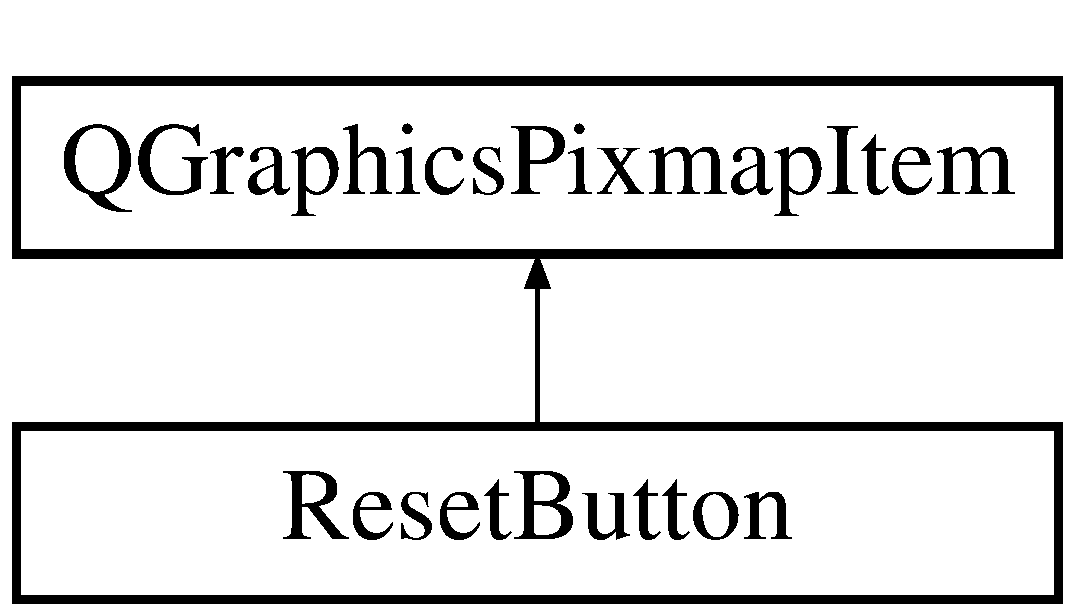
\includegraphics[height=2.000000cm]{class_reset_button}
\end{center}
\end{figure}
\subsection*{Public Member Functions}
\begin{DoxyCompactItemize}
\item 
\hyperlink{class_reset_button_a41e9f93c9b7f758d1791dad20f6a5451}{Reset\+Button} (Q\+Graphics\+Item $\ast$parent=0)
\item 
void \hyperlink{class_reset_button_a21e661fcbc9e266ee9fa76a9feba8401}{mouse\+Press\+Event} (Q\+Graphics\+Scene\+Mouse\+Event $\ast$event)
\end{DoxyCompactItemize}


\subsection{Detailed Description}


Definition at line 7 of file resetbutton.\+h.



\subsection{Constructor \& Destructor Documentation}
\mbox{\Hypertarget{class_reset_button_a41e9f93c9b7f758d1791dad20f6a5451}\label{class_reset_button_a41e9f93c9b7f758d1791dad20f6a5451}} 
\index{Reset\+Button@{Reset\+Button}!Reset\+Button@{Reset\+Button}}
\index{Reset\+Button@{Reset\+Button}!Reset\+Button@{Reset\+Button}}
\subsubsection{\texorpdfstring{Reset\+Button()}{ResetButton()}}
{\footnotesize\ttfamily Reset\+Button\+::\+Reset\+Button (\begin{DoxyParamCaption}\item[{Q\+Graphics\+Item $\ast$}]{parent = {\ttfamily 0} }\end{DoxyParamCaption})}



Definition at line 6 of file resetbutton.\+cpp.


\begin{DoxyCode}
7 \{
8     setPixmap(QPixmap(\textcolor{stringliteral}{":/images/images/reset.png"}));
9 
10 
11 \}
\end{DoxyCode}


\subsection{Member Function Documentation}
\mbox{\Hypertarget{class_reset_button_a21e661fcbc9e266ee9fa76a9feba8401}\label{class_reset_button_a21e661fcbc9e266ee9fa76a9feba8401}} 
\index{Reset\+Button@{Reset\+Button}!mouse\+Press\+Event@{mouse\+Press\+Event}}
\index{mouse\+Press\+Event@{mouse\+Press\+Event}!Reset\+Button@{Reset\+Button}}
\subsubsection{\texorpdfstring{mouse\+Press\+Event()}{mousePressEvent()}}
{\footnotesize\ttfamily void Reset\+Button\+::mouse\+Press\+Event (\begin{DoxyParamCaption}\item[{Q\+Graphics\+Scene\+Mouse\+Event $\ast$}]{event }\end{DoxyParamCaption})}



Definition at line 13 of file resetbutton.\+cpp.


\begin{DoxyCode}
14 \{
15     \hyperlink{resetbutton_8cpp_a58bdb5643d0814ac4e697a1564b79b70}{game}->deleteLater();
16     \hyperlink{resetbutton_8cpp_a58bdb5643d0814ac4e697a1564b79b70}{game} = \textcolor{keyword}{new} \hyperlink{class_game}{Game}();
17     \hyperlink{resetbutton_8cpp_a58bdb5643d0814ac4e697a1564b79b70}{game}->\hyperlink{class_game_af74fd203e3b31917ca9d4769fa608c48}{displayMainMenu}();
18     \hyperlink{resetbutton_8cpp_a58bdb5643d0814ac4e697a1564b79b70}{game}->show();
19 \}
\end{DoxyCode}


The documentation for this class was generated from the following files\+:\begin{DoxyCompactItemize}
\item 
C\+:/\+Users/\+Fu\+Zzy/\+Dropbox/3de Jaar/\+Sem 1/\+R\+E\+I\+I313-\/\+C++ O\+O\+P/\+T\+D\+\_\+\+Game/\+Element\+\_\+\+T\+D/\hyperlink{resetbutton_8h}{resetbutton.\+h}\item 
C\+:/\+Users/\+Fu\+Zzy/\+Dropbox/3de Jaar/\+Sem 1/\+R\+E\+I\+I313-\/\+C++ O\+O\+P/\+T\+D\+\_\+\+Game/\+Element\+\_\+\+T\+D/\hyperlink{resetbutton_8cpp}{resetbutton.\+cpp}\end{DoxyCompactItemize}

\hypertarget{class_sound}{}\section{Sound Class Reference}
\label{class_sound}\index{Sound@{Sound}}


{\ttfamily \#include $<$sound.\+h$>$}

Inheritance diagram for Sound\+:\begin{figure}[H]
\begin{center}
\leavevmode
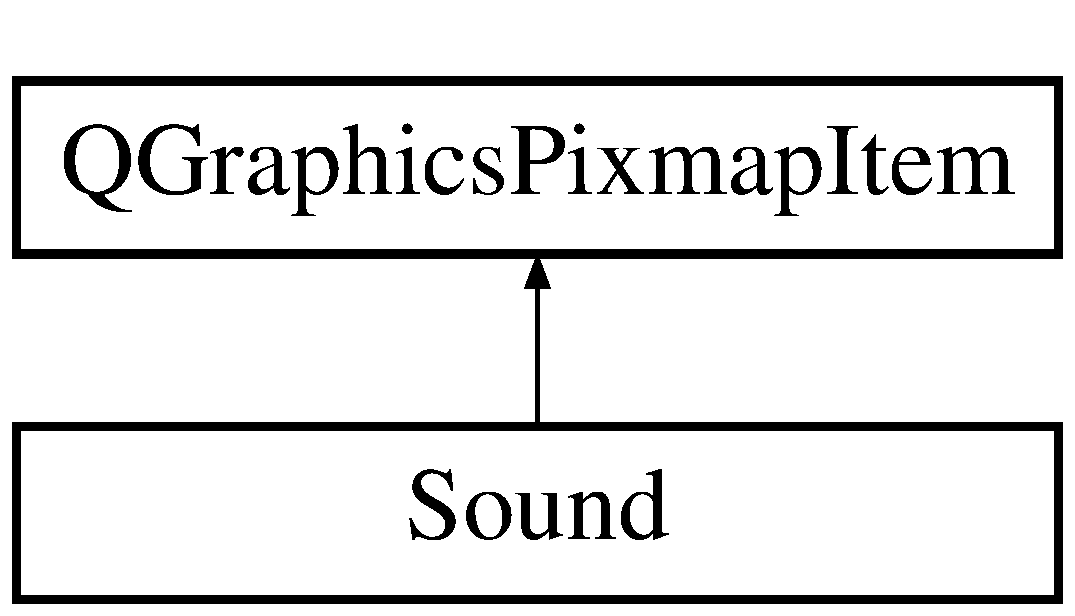
\includegraphics[height=2.000000cm]{class_sound}
\end{center}
\end{figure}
\subsection*{Public Member Functions}
\begin{DoxyCompactItemize}
\item 
\hyperlink{class_sound_a7a36c00590d59181138f371c4cfbe988}{Sound} (Q\+Graphics\+Item $\ast$parent=0)
\item 
void \hyperlink{class_sound_aa145fbdd386c6614d0713802b5c03e07}{mouse\+Press\+Event} (Q\+Graphics\+Scene\+Mouse\+Event $\ast$event)
\end{DoxyCompactItemize}
\subsection*{Private Attributes}
\begin{DoxyCompactItemize}
\item 
bool \hyperlink{class_sound_a8651994f1462748b66bb224e4404c1c0}{playing}
\item 
Q\+Sound $\ast$ \hyperlink{class_sound_a65c0e423d9a706534ed44f4383b5abc1}{theme}
\end{DoxyCompactItemize}


\subsection{Detailed Description}


Definition at line 9 of file sound.\+h.



\subsection{Constructor \& Destructor Documentation}
\mbox{\Hypertarget{class_sound_a7a36c00590d59181138f371c4cfbe988}\label{class_sound_a7a36c00590d59181138f371c4cfbe988}} 
\index{Sound@{Sound}!Sound@{Sound}}
\index{Sound@{Sound}!Sound@{Sound}}
\subsubsection{\texorpdfstring{Sound()}{Sound()}}
{\footnotesize\ttfamily Sound\+::\+Sound (\begin{DoxyParamCaption}\item[{Q\+Graphics\+Item $\ast$}]{parent = {\ttfamily 0} }\end{DoxyParamCaption})}



Definition at line 4 of file sound.\+cpp.


\begin{DoxyCode}
5 \{
6     setPixmap(QPixmap(\textcolor{stringliteral}{":/images/images/sound.png"}));
7 
8     \textcolor{comment}{//play music}
9     \hyperlink{class_sound_a65c0e423d9a706534ed44f4383b5abc1}{theme} = \textcolor{keyword}{new} QSound(\textcolor{stringliteral}{":/images/sounds/Marimba.wav"});
10     \hyperlink{class_sound_a65c0e423d9a706534ed44f4383b5abc1}{theme}->play();
11     \hyperlink{class_sound_a65c0e423d9a706534ed44f4383b5abc1}{theme}->setLoops(QSound::Infinite);
12     \hyperlink{class_sound_a8651994f1462748b66bb224e4404c1c0}{playing} = \textcolor{keyword}{true};
13 
14 \}
\end{DoxyCode}


\subsection{Member Function Documentation}
\mbox{\Hypertarget{class_sound_aa145fbdd386c6614d0713802b5c03e07}\label{class_sound_aa145fbdd386c6614d0713802b5c03e07}} 
\index{Sound@{Sound}!mouse\+Press\+Event@{mouse\+Press\+Event}}
\index{mouse\+Press\+Event@{mouse\+Press\+Event}!Sound@{Sound}}
\subsubsection{\texorpdfstring{mouse\+Press\+Event()}{mousePressEvent()}}
{\footnotesize\ttfamily void Sound\+::mouse\+Press\+Event (\begin{DoxyParamCaption}\item[{Q\+Graphics\+Scene\+Mouse\+Event $\ast$}]{event }\end{DoxyParamCaption})}



Definition at line 16 of file sound.\+cpp.


\begin{DoxyCode}
17 \{
18     \textcolor{keywordflow}{if} (\hyperlink{class_sound_a8651994f1462748b66bb224e4404c1c0}{playing} == \textcolor{keyword}{true}) \{
19         \hyperlink{class_sound_a65c0e423d9a706534ed44f4383b5abc1}{theme}->stop();
20         \hyperlink{class_sound_a8651994f1462748b66bb224e4404c1c0}{playing} = \textcolor{keyword}{false};
21     \}
22     \textcolor{keywordflow}{else}
23     \{
24         \textcolor{comment}{//play music}
25         \hyperlink{class_sound_a65c0e423d9a706534ed44f4383b5abc1}{theme} = \textcolor{keyword}{new} QSound(\textcolor{stringliteral}{":/images/sounds/Marimba.wav"});
26         \hyperlink{class_sound_a65c0e423d9a706534ed44f4383b5abc1}{theme}->play();
27         \hyperlink{class_sound_a65c0e423d9a706534ed44f4383b5abc1}{theme}->setLoops(QSound::Infinite);
28         \hyperlink{class_sound_a8651994f1462748b66bb224e4404c1c0}{playing} = \textcolor{keyword}{true};
29     \}
30 
31 
32 
33 
34 \}
\end{DoxyCode}


\subsection{Member Data Documentation}
\mbox{\Hypertarget{class_sound_a8651994f1462748b66bb224e4404c1c0}\label{class_sound_a8651994f1462748b66bb224e4404c1c0}} 
\index{Sound@{Sound}!playing@{playing}}
\index{playing@{playing}!Sound@{Sound}}
\subsubsection{\texorpdfstring{playing}{playing}}
{\footnotesize\ttfamily bool Sound\+::playing\hspace{0.3cm}{\ttfamily [private]}}



Definition at line 16 of file sound.\+h.

\mbox{\Hypertarget{class_sound_a65c0e423d9a706534ed44f4383b5abc1}\label{class_sound_a65c0e423d9a706534ed44f4383b5abc1}} 
\index{Sound@{Sound}!theme@{theme}}
\index{theme@{theme}!Sound@{Sound}}
\subsubsection{\texorpdfstring{theme}{theme}}
{\footnotesize\ttfamily Q\+Sound$\ast$ Sound\+::theme\hspace{0.3cm}{\ttfamily [private]}}



Definition at line 17 of file sound.\+h.



The documentation for this class was generated from the following files\+:\begin{DoxyCompactItemize}
\item 
C\+:/\+Users/\+Fu\+Zzy/\+Dropbox/3de Jaar/\+Sem 1/\+R\+E\+I\+I313-\/\+C++ O\+O\+P/\+T\+D\+\_\+\+Game/\+Element\+\_\+\+T\+D/\hyperlink{sound_8h}{sound.\+h}\item 
C\+:/\+Users/\+Fu\+Zzy/\+Dropbox/3de Jaar/\+Sem 1/\+R\+E\+I\+I313-\/\+C++ O\+O\+P/\+T\+D\+\_\+\+Game/\+Element\+\_\+\+T\+D/\hyperlink{sound_8cpp}{sound.\+cpp}\end{DoxyCompactItemize}

\hypertarget{class_spawn_eye_icon}{}\section{Spawn\+Eye\+Icon Class Reference}
\label{class_spawn_eye_icon}\index{Spawn\+Eye\+Icon@{Spawn\+Eye\+Icon}}


{\ttfamily \#include $<$spawneyeicon.\+h$>$}

Inheritance diagram for Spawn\+Eye\+Icon\+:\begin{figure}[H]
\begin{center}
\leavevmode
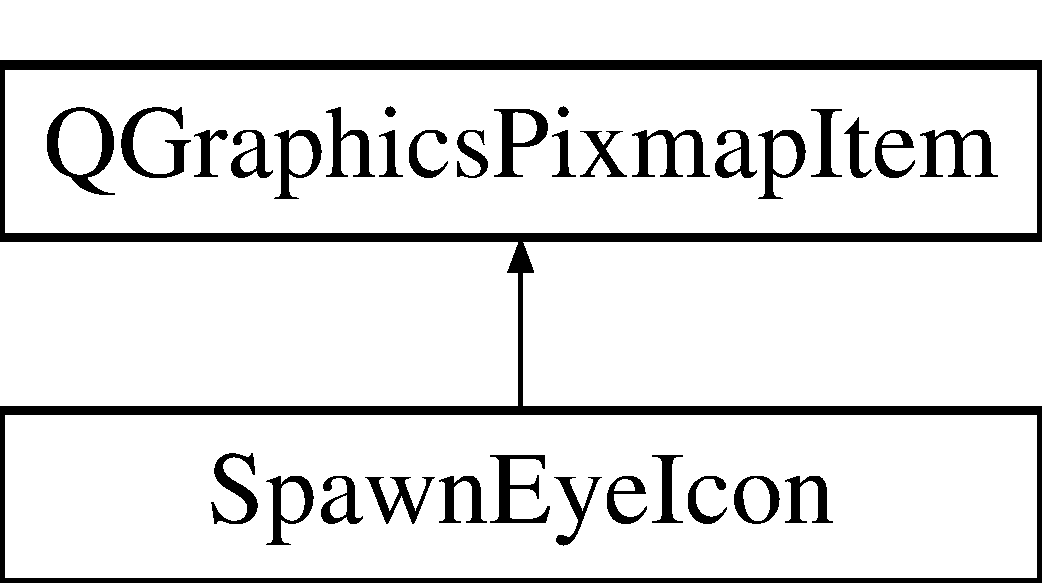
\includegraphics[height=2.000000cm]{class_spawn_eye_icon}
\end{center}
\end{figure}
\subsection*{Public Member Functions}
\begin{DoxyCompactItemize}
\item 
\hyperlink{class_spawn_eye_icon_a89e2b8ca9ce46748cbc2e3d4ad2eddeb}{Spawn\+Eye\+Icon} (Q\+Graphics\+Item $\ast$parent=0)
\item 
void \hyperlink{class_spawn_eye_icon_a7fce32d9b81bdd2a5732372db0c928f0}{mouse\+Press\+Event} (Q\+Graphics\+Scene\+Mouse\+Event $\ast$event)
\end{DoxyCompactItemize}


\subsection{Detailed Description}


Definition at line 7 of file spawneyeicon.\+h.



\subsection{Constructor \& Destructor Documentation}
\mbox{\Hypertarget{class_spawn_eye_icon_a89e2b8ca9ce46748cbc2e3d4ad2eddeb}\label{class_spawn_eye_icon_a89e2b8ca9ce46748cbc2e3d4ad2eddeb}} 
\index{Spawn\+Eye\+Icon@{Spawn\+Eye\+Icon}!Spawn\+Eye\+Icon@{Spawn\+Eye\+Icon}}
\index{Spawn\+Eye\+Icon@{Spawn\+Eye\+Icon}!Spawn\+Eye\+Icon@{Spawn\+Eye\+Icon}}
\subsubsection{\texorpdfstring{Spawn\+Eye\+Icon()}{SpawnEyeIcon()}}
{\footnotesize\ttfamily Spawn\+Eye\+Icon\+::\+Spawn\+Eye\+Icon (\begin{DoxyParamCaption}\item[{Q\+Graphics\+Item $\ast$}]{parent = {\ttfamily 0} }\end{DoxyParamCaption})}



Definition at line 7 of file spawneyeicon.\+cpp.


\begin{DoxyCode}
8 \{
9     setPixmap(QPixmap(\textcolor{stringliteral}{":/images/images/Enemy\_Eye.png"}));
10 \}
\end{DoxyCode}


\subsection{Member Function Documentation}
\mbox{\Hypertarget{class_spawn_eye_icon_a7fce32d9b81bdd2a5732372db0c928f0}\label{class_spawn_eye_icon_a7fce32d9b81bdd2a5732372db0c928f0}} 
\index{Spawn\+Eye\+Icon@{Spawn\+Eye\+Icon}!mouse\+Press\+Event@{mouse\+Press\+Event}}
\index{mouse\+Press\+Event@{mouse\+Press\+Event}!Spawn\+Eye\+Icon@{Spawn\+Eye\+Icon}}
\subsubsection{\texorpdfstring{mouse\+Press\+Event()}{mousePressEvent()}}
{\footnotesize\ttfamily void Spawn\+Eye\+Icon\+::mouse\+Press\+Event (\begin{DoxyParamCaption}\item[{Q\+Graphics\+Scene\+Mouse\+Event $\ast$}]{event }\end{DoxyParamCaption})}



Definition at line 12 of file spawneyeicon.\+cpp.


\begin{DoxyCode}
13 \{
14     \textcolor{comment}{//game->createEnemies(1);}
15     \hyperlink{spawneyeicon_8cpp_a58bdb5643d0814ac4e697a1564b79b70}{game}->\hyperlink{class_game_ad8a7cc146f99c7ec5b7c3c25d73f118c}{player1}->\hyperlink{class_player1_ab390478b345e443398bac442a04b675c}{Gold} += -50;  \textcolor{comment}{//enemy loot value //test code}
16 
17     \textcolor{keywordflow}{if} (\hyperlink{spawneyeicon_8cpp_a58bdb5643d0814ac4e697a1564b79b70}{game}->\hyperlink{class_game_ad8a7cc146f99c7ec5b7c3c25d73f118c}{player1}->\hyperlink{class_player1_ab390478b345e443398bac442a04b675c}{Gold} >= 0) \{
18         \hyperlink{spawneyeicon_8cpp_a58bdb5643d0814ac4e697a1564b79b70}{game}->\hyperlink{class_game_aa7fd8508fad68c550129f2be61c37467}{Client}->\hyperlink{class_u_d_p_socket_a66a6c4663cc3084cb4d76583e8039083}{send}(\textcolor{stringliteral}{"spwn"});
19         \hyperlink{spawneyeicon_8cpp_a58bdb5643d0814ac4e697a1564b79b70}{game}->\hyperlink{class_game_ad8a7cc146f99c7ec5b7c3c25d73f118c}{player1}->\hyperlink{class_player1_a414fae948c79246f6a98554718f0cd99}{Income} += 5;
20         \hyperlink{spawneyeicon_8cpp_a58bdb5643d0814ac4e697a1564b79b70}{game}->\hyperlink{class_game_a5a6924497d779286af09f339d4c7a598}{updateIncome}();
21         \hyperlink{spawneyeicon_8cpp_a58bdb5643d0814ac4e697a1564b79b70}{game}->\hyperlink{class_game_a065998f7609f63e2987ede928359595a}{updateGold}();
22     \}
23     \textcolor{keywordflow}{else}
24     \{
25         \hyperlink{spawneyeicon_8cpp_a58bdb5643d0814ac4e697a1564b79b70}{game}->\hyperlink{class_game_ad8a7cc146f99c7ec5b7c3c25d73f118c}{player1}->\hyperlink{class_player1_ab390478b345e443398bac442a04b675c}{Gold} += 50;
26         \textcolor{keywordflow}{return};
27     \}
28 
29 
30 \}
\end{DoxyCode}


The documentation for this class was generated from the following files\+:\begin{DoxyCompactItemize}
\item 
C\+:/\+Users/\+Fu\+Zzy/\+Dropbox/3de Jaar/\+Sem 1/\+R\+E\+I\+I313-\/\+C++ O\+O\+P/\+T\+D\+\_\+\+Game/\+Element\+\_\+\+T\+D/\hyperlink{spawneyeicon_8h}{spawneyeicon.\+h}\item 
C\+:/\+Users/\+Fu\+Zzy/\+Dropbox/3de Jaar/\+Sem 1/\+R\+E\+I\+I313-\/\+C++ O\+O\+P/\+T\+D\+\_\+\+Game/\+Element\+\_\+\+T\+D/\hyperlink{spawneyeicon_8cpp}{spawneyeicon.\+cpp}\end{DoxyCompactItemize}

\hypertarget{class_tower}{}\section{Tower Class Reference}
\label{class_tower}\index{Tower@{Tower}}


{\ttfamily \#include $<$tower.\+h$>$}

Inheritance diagram for Tower\+:\begin{figure}[H]
\begin{center}
\leavevmode
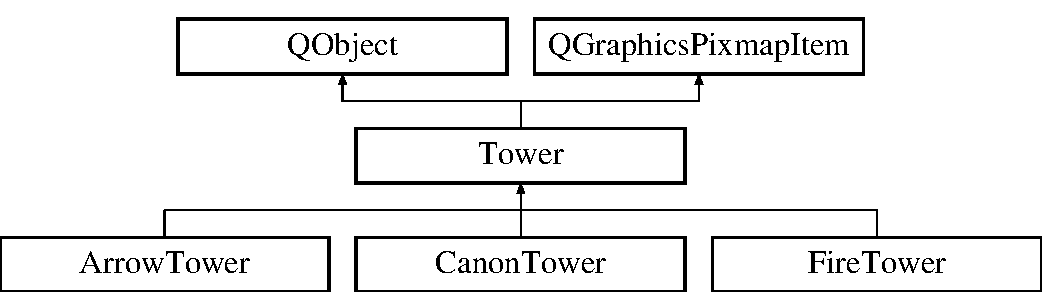
\includegraphics[height=3.000000cm]{class_tower}
\end{center}
\end{figure}
\subsection*{Public Slots}
\begin{DoxyCompactItemize}
\item 
void \hyperlink{class_tower_a6e0df1e43e746622967918aaf6f42dce}{aquire\+\_\+target} ()
\end{DoxyCompactItemize}
\subsection*{Public Member Functions}
\begin{DoxyCompactItemize}
\item 
\hyperlink{class_tower_aa3ff2c932ed113a80a122dbe2e3e0176}{Tower} (Q\+Graphics\+Item $\ast$parent=0)
\item 
double \hyperlink{class_tower_a1b04543304dcd92cee3c0909362a9a3f}{distance\+To} (Q\+Graphics\+Item $\ast$item)
\item 
virtual void \hyperlink{class_tower_a11d4b8069b148e8587b2e7bc2d68b55d}{mouse\+Press\+Event} (Q\+Mouse\+Event $\ast$event)
\item 
virtual void \hyperlink{class_tower_aa0c9c780f48cffacd3da6877f5d4fdc2}{fire} ()
\item 
virtual int \hyperlink{class_tower_ae1d3f44d0149c8146ccf6b262a52ddad}{get\+Cost\+Of\+Tower} ()
\item 
virtual void \hyperlink{class_tower_a7736b1132e64e14a977e9e8c91c3338f}{sell\+Tower} ()
\item 
bool \hyperlink{class_tower_a7632139d282286858bcf80fa0044e19b}{get\+Is\+Placed} ()
\item 
Q\+String \hyperlink{class_tower_a36d5430c311d9e0509c1c078ca1876dc}{get\+Owner} ()
\item 
void \hyperlink{class_tower_aaab33d438ff21a9628534b0e027fe4f7}{set\+Is\+Placed} (bool b)
\item 
void \hyperlink{class_tower_a2c56faabb6910f6dadddf61b1decdbf9}{set\+Owner} (Q\+String player)
\end{DoxyCompactItemize}
\subsection*{Public Attributes}
\begin{DoxyCompactItemize}
\item 
const int \hyperlink{class_tower_ac97e0d44e295399c5cac3cc6e2060df6}{cost\+Of\+Tower} = 50
\end{DoxyCompactItemize}
\subsection*{Protected Attributes}
\begin{DoxyCompactItemize}
\item 
bool \hyperlink{class_tower_a1317cf5400c63351e0d66b17df5c0417}{is\+Placed} = false
\item 
Q\+String \hyperlink{class_tower_abff7e8aaf637c17bcba08f9097db38df}{owner}
\item 
Q\+Graphics\+Polygon\+Item $\ast$ \hyperlink{class_tower_a628af042db1aa134f2ab18b1f2b0eeb9}{attack\+\_\+area}
\item 
bool \hyperlink{class_tower_a568b9b12bc604fb245a79476b71d6557}{has\+\_\+target}
\item 
Q\+PointF \hyperlink{class_tower_a2b3e8ab90ccceed1fa3a667db80c2c06}{attack\+\_\+dest}
\end{DoxyCompactItemize}


\subsection{Detailed Description}


Definition at line 11 of file tower.\+h.



\subsection{Constructor \& Destructor Documentation}
\mbox{\Hypertarget{class_tower_aa3ff2c932ed113a80a122dbe2e3e0176}\label{class_tower_aa3ff2c932ed113a80a122dbe2e3e0176}} 
\index{Tower@{Tower}!Tower@{Tower}}
\index{Tower@{Tower}!Tower@{Tower}}
\subsubsection{\texorpdfstring{Tower()}{Tower()}}
{\footnotesize\ttfamily Tower\+::\+Tower (\begin{DoxyParamCaption}\item[{Q\+Graphics\+Item $\ast$}]{parent = {\ttfamily 0} }\end{DoxyParamCaption})}



Definition at line 18 of file tower.\+cpp.


\begin{DoxyCode}
18                                  :QObject(), QGraphicsPixmapItem(parent)
19 \{
20     \textcolor{comment}{//set the graphics}
21     setPixmap(QPixmap(\textcolor{stringliteral}{":/images/images/Tower\_Arrow.png"}));
22     \textcolor{keywordtype}{int} w = pixmap().width();
23     \textcolor{keywordtype}{int} h = pixmap().height();
24     setOffset(-w/2,-h/1.25);
25 
26     \textcolor{comment}{//create points vector}
27     QVector<QPointF> points;
28     points << QPoint(1,0) << QPoint(2,0) << QPoint(3,1) << QPoint(3,2) << QPoint(2,3) << QPoint(1,3)
29            << QPoint(0,2) << QPoint(0,1);
30 
31     \textcolor{comment}{//scale points}
32     \textcolor{keywordtype}{int} SCALE\_FACTOR = pixmap().width();
33     \textcolor{keywordflow}{for} (\textcolor{keywordtype}{size\_t} i=0 , n = points.size() ;i<n ; i++)
34     \{
35         points[i] *= SCALE\_FACTOR;
36     \}
37 
38     \textcolor{comment}{//create polygon from these points}
39     QPolygonF polygon(points);
40 
41     \textcolor{comment}{//create the polyitem}
42     \hyperlink{class_tower_a628af042db1aa134f2ab18b1f2b0eeb9}{attack\_area} = \textcolor{keyword}{new} QGraphicsPolygonItem(polygon,\textcolor{keyword}{this});
43     \hyperlink{class_tower_a628af042db1aa134f2ab18b1f2b0eeb9}{attack\_area}->setPen(QPen(Qt::DotLine));
44 
45     \textcolor{comment}{//move the polygon}
46     QPointF poly\_center(1.5,1.5);
47     poly\_center *= SCALE\_FACTOR;
48     poly\_center = mapToScene(poly\_center);
49     QPointF tower\_center(x(),y());
50     QLineF ln(poly\_center,tower\_center);
51     \hyperlink{class_tower_a628af042db1aa134f2ab18b1f2b0eeb9}{attack\_area}->setPos(x()+ln.dx(),y()+ln.dy());
52 
53     \textcolor{comment}{//set attack dest}
54     \hyperlink{class_tower_a2b3e8ab90ccceed1fa3a667db80c2c06}{attack\_dest} = QPointF(0,0);
55     \hyperlink{class_tower_a568b9b12bc604fb245a79476b71d6557}{has\_target} = \textcolor{keyword}{false};
56 
57 \}
\end{DoxyCode}


\subsection{Member Function Documentation}
\mbox{\Hypertarget{class_tower_a6e0df1e43e746622967918aaf6f42dce}\label{class_tower_a6e0df1e43e746622967918aaf6f42dce}} 
\index{Tower@{Tower}!aquire\+\_\+target@{aquire\+\_\+target}}
\index{aquire\+\_\+target@{aquire\+\_\+target}!Tower@{Tower}}
\subsubsection{\texorpdfstring{aquire\+\_\+target}{aquire\_target}}
{\footnotesize\ttfamily void Tower\+::aquire\+\_\+target (\begin{DoxyParamCaption}{ }\end{DoxyParamCaption})\hspace{0.3cm}{\ttfamily [slot]}}



Definition at line 123 of file tower.\+cpp.


\begin{DoxyCode}
124 \{
125     \textcolor{comment}{// get a list of all enemies that collide with attack\_area, find the closest one}
126     \textcolor{comment}{// and set it's position as the attack\_dest}
127 
128     \textcolor{comment}{// get a list of all enemies within attack\_area}
129     QList<QGraphicsItem *> colliding\_items = \hyperlink{class_tower_a628af042db1aa134f2ab18b1f2b0eeb9}{attack\_area}->collidingItems();
130 
131     \textcolor{comment}{// assume tower does not have a target, unless we find one}
132     \hyperlink{class_tower_a568b9b12bc604fb245a79476b71d6557}{has\_target} = \textcolor{keyword}{false};
133 
134     \textcolor{comment}{//find the closest enemy}
135     \textcolor{keywordtype}{double} closest\_dist = 300;
136     QPointF closest\_pt(0,0);
137     \textcolor{keywordflow}{for} ( \textcolor{keywordtype}{size\_t} i = 0, n = colliding\_items.size(); i <n ; i++)
138     \{
139         \textcolor{comment}{//make sure it is an enemy}
140         \hyperlink{class_enemy}{Enemy} * enemy = \textcolor{keyword}{dynamic\_cast<}\hyperlink{class_enemy}{Enemy} *\textcolor{keyword}{>}(colliding\_items[i]);
141 
142         \textcolor{comment}{//see if distance is closer}
143         \textcolor{keywordflow}{if} (enemy) \{
144             \textcolor{keywordtype}{double} this\_dist = \hyperlink{class_tower_a1b04543304dcd92cee3c0909362a9a3f}{distanceTo}(colliding\_items[i]);
145             \textcolor{keywordflow}{if} (this\_dist < closest\_dist) \{
146                 closest\_dist = this\_dist;
147                 closest\_pt = colliding\_items[i]->pos();\textcolor{comment}{//speel met die pos om center van enemy te kry}
148                 \hyperlink{class_tower_a568b9b12bc604fb245a79476b71d6557}{has\_target} = \textcolor{keyword}{true};
149             \}
150         \}
151     \}
152 
153     \textcolor{comment}{//if has target, set the closest enemy as the attack\_dest, and fire}
154     \textcolor{keywordflow}{if} (\hyperlink{class_tower_a568b9b12bc604fb245a79476b71d6557}{has\_target} == \textcolor{keyword}{true})
155     \{
156         \hyperlink{class_tower_a2b3e8ab90ccceed1fa3a667db80c2c06}{attack\_dest} = closest\_pt;
157         \hyperlink{class_tower_aa0c9c780f48cffacd3da6877f5d4fdc2}{fire}();
158     \}
159 \}
\end{DoxyCode}
\mbox{\Hypertarget{class_tower_a1b04543304dcd92cee3c0909362a9a3f}\label{class_tower_a1b04543304dcd92cee3c0909362a9a3f}} 
\index{Tower@{Tower}!distance\+To@{distance\+To}}
\index{distance\+To@{distance\+To}!Tower@{Tower}}
\subsubsection{\texorpdfstring{distance\+To()}{distanceTo()}}
{\footnotesize\ttfamily double Tower\+::distance\+To (\begin{DoxyParamCaption}\item[{Q\+Graphics\+Item $\ast$}]{item }\end{DoxyParamCaption})}



Definition at line 59 of file tower.\+cpp.


\begin{DoxyCode}
60 \{
61     QLineF ln(pos(), item->pos());
62     \textcolor{keywordflow}{return} ln.length();
63 \}
\end{DoxyCode}
\mbox{\Hypertarget{class_tower_aa0c9c780f48cffacd3da6877f5d4fdc2}\label{class_tower_aa0c9c780f48cffacd3da6877f5d4fdc2}} 
\index{Tower@{Tower}!fire@{fire}}
\index{fire@{fire}!Tower@{Tower}}
\subsubsection{\texorpdfstring{fire()}{fire()}}
{\footnotesize\ttfamily void Tower\+::fire (\begin{DoxyParamCaption}{ }\end{DoxyParamCaption})\hspace{0.3cm}{\ttfamily [virtual]}}



Reimplemented in \hyperlink{class_arrow_tower_ab4ed87128b5037a98640ab05e8721d88}{Arrow\+Tower}, \hyperlink{class_canon_tower_aa8d13cf8b8d530256b95746620e16234}{Canon\+Tower}, and \hyperlink{class_fire_tower_a9a0b13fcb0bc204194d953c5494afbe3}{Fire\+Tower}.



Definition at line 78 of file tower.\+cpp.


\begin{DoxyCode}
79 \{
80     \hyperlink{class_bullet}{Bullet} *bullet = \textcolor{keyword}{new} \hyperlink{class_bullet}{Bullet}();
81     \textcolor{keywordtype}{int} y\_pos = pixmap().height()*\hyperlink{tower_8cpp_a58bdb5643d0814ac4e697a1564b79b70}{game}->\hyperlink{class_game_a6c1ca48f17f6934432d01bfa7f762a04}{scalingfactor\_towers}/1.25;
82 
83     bullet->setPos(x(), y()-y\_pos);
84 
85     QLineF ln(QPointF(x(), y()-y\_pos),\hyperlink{class_tower_a2b3e8ab90ccceed1fa3a667db80c2c06}{attack\_dest});
86     \textcolor{keywordtype}{int} angle = -1*ln.angle();
87 
88     bullet->setRotation(angle);
89     \hyperlink{tower_8cpp_a58bdb5643d0814ac4e697a1564b79b70}{game}->\hyperlink{class_game_a8119e3b9a632906c6808fa294b46a92a}{scene}->addItem(bullet);
90 \}
\end{DoxyCode}
\mbox{\Hypertarget{class_tower_ae1d3f44d0149c8146ccf6b262a52ddad}\label{class_tower_ae1d3f44d0149c8146ccf6b262a52ddad}} 
\index{Tower@{Tower}!get\+Cost\+Of\+Tower@{get\+Cost\+Of\+Tower}}
\index{get\+Cost\+Of\+Tower@{get\+Cost\+Of\+Tower}!Tower@{Tower}}
\subsubsection{\texorpdfstring{get\+Cost\+Of\+Tower()}{getCostOfTower()}}
{\footnotesize\ttfamily int Tower\+::get\+Cost\+Of\+Tower (\begin{DoxyParamCaption}{ }\end{DoxyParamCaption})\hspace{0.3cm}{\ttfamily [virtual]}}



Reimplemented in \hyperlink{class_arrow_tower_a1ef82141056a39071f89d1c360728116}{Arrow\+Tower}, \hyperlink{class_canon_tower_ac0e57d350da509e89e926afe950ab291}{Canon\+Tower}, and \hyperlink{class_fire_tower_a74be102e9bb0871f19fb55b434e2b6d7}{Fire\+Tower}.



Definition at line 92 of file tower.\+cpp.


\begin{DoxyCode}
93 \{
94     \textcolor{keywordflow}{return} \hyperlink{class_tower_ac97e0d44e295399c5cac3cc6e2060df6}{costOfTower};
95 \}
\end{DoxyCode}
\mbox{\Hypertarget{class_tower_a7632139d282286858bcf80fa0044e19b}\label{class_tower_a7632139d282286858bcf80fa0044e19b}} 
\index{Tower@{Tower}!get\+Is\+Placed@{get\+Is\+Placed}}
\index{get\+Is\+Placed@{get\+Is\+Placed}!Tower@{Tower}}
\subsubsection{\texorpdfstring{get\+Is\+Placed()}{getIsPlaced()}}
{\footnotesize\ttfamily bool Tower\+::get\+Is\+Placed (\begin{DoxyParamCaption}{ }\end{DoxyParamCaption})}



Definition at line 103 of file tower.\+cpp.


\begin{DoxyCode}
104 \{
105     \textcolor{keywordflow}{return} \hyperlink{class_tower_a1317cf5400c63351e0d66b17df5c0417}{isPlaced};
106 \}
\end{DoxyCode}
\mbox{\Hypertarget{class_tower_a36d5430c311d9e0509c1c078ca1876dc}\label{class_tower_a36d5430c311d9e0509c1c078ca1876dc}} 
\index{Tower@{Tower}!get\+Owner@{get\+Owner}}
\index{get\+Owner@{get\+Owner}!Tower@{Tower}}
\subsubsection{\texorpdfstring{get\+Owner()}{getOwner()}}
{\footnotesize\ttfamily Q\+String Tower\+::get\+Owner (\begin{DoxyParamCaption}{ }\end{DoxyParamCaption})}



Definition at line 108 of file tower.\+cpp.


\begin{DoxyCode}
109 \{
110     \textcolor{keywordflow}{return} \hyperlink{class_tower_abff7e8aaf637c17bcba08f9097db38df}{owner};
111 \}
\end{DoxyCode}
\mbox{\Hypertarget{class_tower_a11d4b8069b148e8587b2e7bc2d68b55d}\label{class_tower_a11d4b8069b148e8587b2e7bc2d68b55d}} 
\index{Tower@{Tower}!mouse\+Press\+Event@{mouse\+Press\+Event}}
\index{mouse\+Press\+Event@{mouse\+Press\+Event}!Tower@{Tower}}
\subsubsection{\texorpdfstring{mouse\+Press\+Event()}{mousePressEvent()}}
{\footnotesize\ttfamily void Tower\+::mouse\+Press\+Event (\begin{DoxyParamCaption}\item[{Q\+Mouse\+Event $\ast$}]{event }\end{DoxyParamCaption})\hspace{0.3cm}{\ttfamily [virtual]}}



Definition at line 65 of file tower.\+cpp.


\begin{DoxyCode}
66 \{
67     qDebug() << \textcolor{stringliteral}{"Tower Clicked"};
68     \textcolor{keywordflow}{if} (event->button() == Qt::RightButton) \{
69         \hyperlink{class_tower_a7736b1132e64e14a977e9e8c91c3338f}{sellTower}();
70     \}
71     \textcolor{keywordflow}{else}
72     \{
73 \textcolor{comment}{//        QGraphicsView::mousePressEvent(event);}
74         \textcolor{keywordflow}{return};
75     \}
76 \}
\end{DoxyCode}
\mbox{\Hypertarget{class_tower_a7736b1132e64e14a977e9e8c91c3338f}\label{class_tower_a7736b1132e64e14a977e9e8c91c3338f}} 
\index{Tower@{Tower}!sell\+Tower@{sell\+Tower}}
\index{sell\+Tower@{sell\+Tower}!Tower@{Tower}}
\subsubsection{\texorpdfstring{sell\+Tower()}{sellTower()}}
{\footnotesize\ttfamily void Tower\+::sell\+Tower (\begin{DoxyParamCaption}{ }\end{DoxyParamCaption})\hspace{0.3cm}{\ttfamily [virtual]}}



Reimplemented in \hyperlink{class_arrow_tower_a7ac5bf2863d8a4c461d26a3a60dc62ab}{Arrow\+Tower}, \hyperlink{class_canon_tower_a5bfc0567c8907e8a6ddf4722f6783cd0}{Canon\+Tower}, and \hyperlink{class_fire_tower_adc1bcb15312eac1dd9788be48e55baad}{Fire\+Tower}.



Definition at line 97 of file tower.\+cpp.


\begin{DoxyCode}
98 \{
99     \textcolor{comment}{//sell hier?}
100     qDebug() << \textcolor{stringliteral}{"Sold!"};
101 \}
\end{DoxyCode}
\mbox{\Hypertarget{class_tower_aaab33d438ff21a9628534b0e027fe4f7}\label{class_tower_aaab33d438ff21a9628534b0e027fe4f7}} 
\index{Tower@{Tower}!set\+Is\+Placed@{set\+Is\+Placed}}
\index{set\+Is\+Placed@{set\+Is\+Placed}!Tower@{Tower}}
\subsubsection{\texorpdfstring{set\+Is\+Placed()}{setIsPlaced()}}
{\footnotesize\ttfamily void Tower\+::set\+Is\+Placed (\begin{DoxyParamCaption}\item[{bool}]{b }\end{DoxyParamCaption})}



Definition at line 113 of file tower.\+cpp.


\begin{DoxyCode}
114 \{
115     \hyperlink{class_tower_a1317cf5400c63351e0d66b17df5c0417}{isPlaced} = b;
116 \}
\end{DoxyCode}
\mbox{\Hypertarget{class_tower_a2c56faabb6910f6dadddf61b1decdbf9}\label{class_tower_a2c56faabb6910f6dadddf61b1decdbf9}} 
\index{Tower@{Tower}!set\+Owner@{set\+Owner}}
\index{set\+Owner@{set\+Owner}!Tower@{Tower}}
\subsubsection{\texorpdfstring{set\+Owner()}{setOwner()}}
{\footnotesize\ttfamily void Tower\+::set\+Owner (\begin{DoxyParamCaption}\item[{Q\+String}]{player }\end{DoxyParamCaption})}



Definition at line 118 of file tower.\+cpp.


\begin{DoxyCode}
119 \{
120     \hyperlink{class_tower_abff7e8aaf637c17bcba08f9097db38df}{owner} = player;
121 \}
\end{DoxyCode}


\subsection{Member Data Documentation}
\mbox{\Hypertarget{class_tower_a628af042db1aa134f2ab18b1f2b0eeb9}\label{class_tower_a628af042db1aa134f2ab18b1f2b0eeb9}} 
\index{Tower@{Tower}!attack\+\_\+area@{attack\+\_\+area}}
\index{attack\+\_\+area@{attack\+\_\+area}!Tower@{Tower}}
\subsubsection{\texorpdfstring{attack\+\_\+area}{attack\_area}}
{\footnotesize\ttfamily Q\+Graphics\+Polygon\+Item$\ast$ Tower\+::attack\+\_\+area\hspace{0.3cm}{\ttfamily [protected]}}



Definition at line 43 of file tower.\+h.

\mbox{\Hypertarget{class_tower_a2b3e8ab90ccceed1fa3a667db80c2c06}\label{class_tower_a2b3e8ab90ccceed1fa3a667db80c2c06}} 
\index{Tower@{Tower}!attack\+\_\+dest@{attack\+\_\+dest}}
\index{attack\+\_\+dest@{attack\+\_\+dest}!Tower@{Tower}}
\subsubsection{\texorpdfstring{attack\+\_\+dest}{attack\_dest}}
{\footnotesize\ttfamily Q\+PointF Tower\+::attack\+\_\+dest\hspace{0.3cm}{\ttfamily [protected]}}



Definition at line 45 of file tower.\+h.

\mbox{\Hypertarget{class_tower_ac97e0d44e295399c5cac3cc6e2060df6}\label{class_tower_ac97e0d44e295399c5cac3cc6e2060df6}} 
\index{Tower@{Tower}!cost\+Of\+Tower@{cost\+Of\+Tower}}
\index{cost\+Of\+Tower@{cost\+Of\+Tower}!Tower@{Tower}}
\subsubsection{\texorpdfstring{cost\+Of\+Tower}{costOfTower}}
{\footnotesize\ttfamily const int Tower\+::cost\+Of\+Tower = 50}



Definition at line 21 of file tower.\+h.

\mbox{\Hypertarget{class_tower_a568b9b12bc604fb245a79476b71d6557}\label{class_tower_a568b9b12bc604fb245a79476b71d6557}} 
\index{Tower@{Tower}!has\+\_\+target@{has\+\_\+target}}
\index{has\+\_\+target@{has\+\_\+target}!Tower@{Tower}}
\subsubsection{\texorpdfstring{has\+\_\+target}{has\_target}}
{\footnotesize\ttfamily bool Tower\+::has\+\_\+target\hspace{0.3cm}{\ttfamily [protected]}}



Definition at line 44 of file tower.\+h.

\mbox{\Hypertarget{class_tower_a1317cf5400c63351e0d66b17df5c0417}\label{class_tower_a1317cf5400c63351e0d66b17df5c0417}} 
\index{Tower@{Tower}!is\+Placed@{is\+Placed}}
\index{is\+Placed@{is\+Placed}!Tower@{Tower}}
\subsubsection{\texorpdfstring{is\+Placed}{isPlaced}}
{\footnotesize\ttfamily bool Tower\+::is\+Placed = false\hspace{0.3cm}{\ttfamily [protected]}}



Definition at line 38 of file tower.\+h.

\mbox{\Hypertarget{class_tower_abff7e8aaf637c17bcba08f9097db38df}\label{class_tower_abff7e8aaf637c17bcba08f9097db38df}} 
\index{Tower@{Tower}!owner@{owner}}
\index{owner@{owner}!Tower@{Tower}}
\subsubsection{\texorpdfstring{owner}{owner}}
{\footnotesize\ttfamily Q\+String Tower\+::owner\hspace{0.3cm}{\ttfamily [protected]}}



Definition at line 39 of file tower.\+h.



The documentation for this class was generated from the following files\+:\begin{DoxyCompactItemize}
\item 
C\+:/\+Users/\+Fu\+Zzy/\+Dropbox/3de Jaar/\+Sem 1/\+R\+E\+I\+I313-\/\+C++ O\+O\+P/\+T\+D\+\_\+\+Game/\+Element\+\_\+\+T\+D/\hyperlink{tower_8h}{tower.\+h}\item 
C\+:/\+Users/\+Fu\+Zzy/\+Dropbox/3de Jaar/\+Sem 1/\+R\+E\+I\+I313-\/\+C++ O\+O\+P/\+T\+D\+\_\+\+Game/\+Element\+\_\+\+T\+D/\hyperlink{tower_8cpp}{tower.\+cpp}\end{DoxyCompactItemize}

\hypertarget{class_u_d_p_class}{}\section{U\+D\+P\+Class Class Reference}
\label{class_u_d_p_class}\index{U\+D\+P\+Class@{U\+D\+P\+Class}}


{\ttfamily \#include $<$udpclass.\+h$>$}

\subsection*{Public Member Functions}
\begin{DoxyCompactItemize}
\item 
\hyperlink{class_u_d_p_class_aea79eb2fa6dccf4a5418b37625b1b9b2}{U\+D\+P\+Class} ()
\end{DoxyCompactItemize}


\subsection{Detailed Description}


Definition at line 5 of file udpclass.\+h.



\subsection{Constructor \& Destructor Documentation}
\mbox{\Hypertarget{class_u_d_p_class_aea79eb2fa6dccf4a5418b37625b1b9b2}\label{class_u_d_p_class_aea79eb2fa6dccf4a5418b37625b1b9b2}} 
\index{U\+D\+P\+Class@{U\+D\+P\+Class}!U\+D\+P\+Class@{U\+D\+P\+Class}}
\index{U\+D\+P\+Class@{U\+D\+P\+Class}!U\+D\+P\+Class@{U\+D\+P\+Class}}
\subsubsection{\texorpdfstring{U\+D\+P\+Class()}{UDPClass()}}
{\footnotesize\ttfamily U\+D\+P\+Class\+::\+U\+D\+P\+Class (\begin{DoxyParamCaption}{ }\end{DoxyParamCaption})}



Definition at line 3 of file udpclass.\+cpp.


\begin{DoxyCode}
4 \{
5 
6 \}
\end{DoxyCode}


The documentation for this class was generated from the following files\+:\begin{DoxyCompactItemize}
\item 
C\+:/\+Users/\+Fu\+Zzy/\+Dropbox/3de Jaar/\+Sem 1/\+R\+E\+I\+I313-\/\+C++ O\+O\+P/\+T\+D\+\_\+\+Game/\+Element\+\_\+\+T\+D/\hyperlink{udpclass_8h}{udpclass.\+h}\item 
C\+:/\+Users/\+Fu\+Zzy/\+Dropbox/3de Jaar/\+Sem 1/\+R\+E\+I\+I313-\/\+C++ O\+O\+P/\+T\+D\+\_\+\+Game/\+Element\+\_\+\+T\+D/\hyperlink{udpclass_8cpp}{udpclass.\+cpp}\end{DoxyCompactItemize}

\hypertarget{class_u_d_p_socket}{}\section{U\+D\+P\+Socket Class Reference}
\label{class_u_d_p_socket}\index{U\+D\+P\+Socket@{U\+D\+P\+Socket}}


{\ttfamily \#include $<$udpsocket.\+h$>$}

Inheritance diagram for U\+D\+P\+Socket\+:\begin{figure}[H]
\begin{center}
\leavevmode
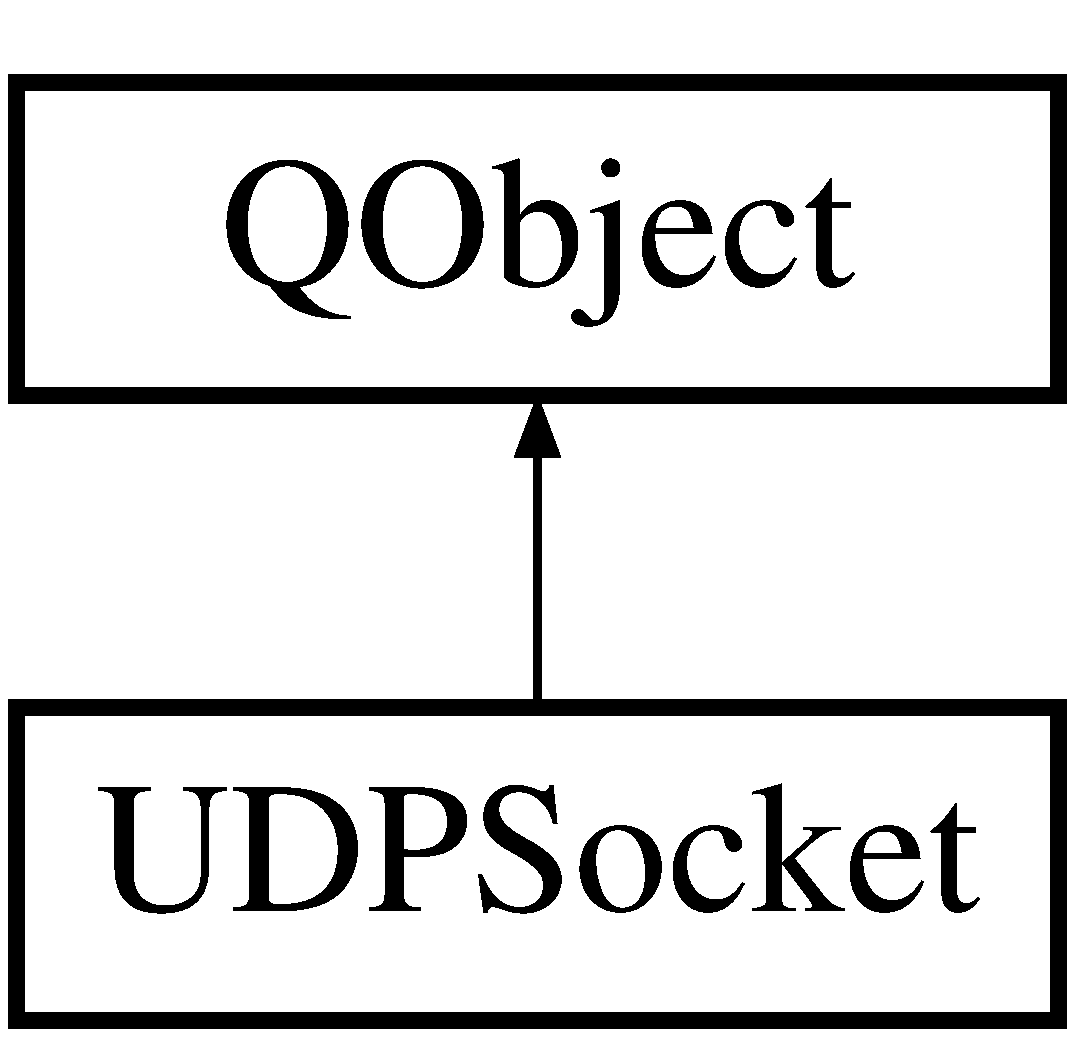
\includegraphics[height=2.000000cm]{class_u_d_p_socket}
\end{center}
\end{figure}
\subsection*{Public Member Functions}
\begin{DoxyCompactItemize}
\item 
\hyperlink{class_u_d_p_socket_a3d40509e1eb916df5ecbca4d3696c3d2}{U\+D\+P\+Socket} (Q\+Object $\ast$parent=0)
\item 
void \hyperlink{class_u_d_p_socket_a991e20366ed560c24402d7a6404daea7}{say\+Hello} ()
\item 
void \hyperlink{class_u_d_p_socket_a66a6c4663cc3084cb4d76583e8039083}{send} (Q\+String str)
\item 
void \hyperlink{class_u_d_p_socket_ad84c799182b7d7edafe956674ecb3faf}{process\+The\+Datagram} (Q\+Network\+Datagram datagram)
\item 
void \hyperlink{class_u_d_p_socket_a9cfc381ef8fe97d2adea9eb0d2c2c1f5}{emit\+IP} ()
\item 
Q\+Host\+Address \hyperlink{class_u_d_p_socket_a8d1b7ad860447197ac896f35949aa723}{get\+Host\+Adress} () const
\item 
void \hyperlink{class_u_d_p_socket_a5bdac3040e57d37c503fdd3293b6d053}{set\+Host\+Adress} (const Q\+Host\+Address \&value)
\end{DoxyCompactItemize}
\subsection*{Public Attributes}
\begin{DoxyCompactItemize}
\item 
Q\+Host\+Address \hyperlink{class_u_d_p_socket_aacd808913633488ab008e8aa7ff8d9cf}{host\+Adress}
\end{DoxyCompactItemize}
\subsection*{Private Slots}
\begin{DoxyCompactItemize}
\item 
void \hyperlink{class_u_d_p_socket_a927f0446edc240955bea6e6e493e6621}{read\+Pending\+Datagrams} ()
\end{DoxyCompactItemize}
\subsection*{Private Attributes}
\begin{DoxyCompactItemize}
\item 
Q\+Udp\+Socket $\ast$ \hyperlink{class_u_d_p_socket_a9d27cb09deee765dfec056cfc774c878}{socket}
\end{DoxyCompactItemize}


\subsection{Detailed Description}


Definition at line 8 of file udpsocket.\+h.



\subsection{Constructor \& Destructor Documentation}
\mbox{\Hypertarget{class_u_d_p_socket_a3d40509e1eb916df5ecbca4d3696c3d2}\label{class_u_d_p_socket_a3d40509e1eb916df5ecbca4d3696c3d2}} 
\index{U\+D\+P\+Socket@{U\+D\+P\+Socket}!U\+D\+P\+Socket@{U\+D\+P\+Socket}}
\index{U\+D\+P\+Socket@{U\+D\+P\+Socket}!U\+D\+P\+Socket@{U\+D\+P\+Socket}}
\subsubsection{\texorpdfstring{U\+D\+P\+Socket()}{UDPSocket()}}
{\footnotesize\ttfamily U\+D\+P\+Socket\+::\+U\+D\+P\+Socket (\begin{DoxyParamCaption}\item[{Q\+Object $\ast$}]{parent = {\ttfamily 0} }\end{DoxyParamCaption})\hspace{0.3cm}{\ttfamily [explicit]}}



Definition at line 8 of file udpsocket.\+cpp.


\begin{DoxyCode}
8                                     : QObject(parent)
9 \{
10     \hyperlink{class_u_d_p_socket_a9d27cb09deee765dfec056cfc774c878}{socket} = \textcolor{keyword}{new} QUdpSocket(\textcolor{keyword}{this});
11     connect(\hyperlink{class_u_d_p_socket_a9d27cb09deee765dfec056cfc774c878}{socket}, SIGNAL(readyRead()), \textcolor{keyword}{this}, SLOT(\hyperlink{class_u_d_p_socket_a927f0446edc240955bea6e6e493e6621}{readPendingDatagrams}()));
12     \hyperlink{class_u_d_p_socket_a9d27cb09deee765dfec056cfc774c878}{socket}->bind(700);
13 
14     \textcolor{comment}{//default}
15     \hyperlink{class_u_d_p_socket_aacd808913633488ab008e8aa7ff8d9cf}{hostAdress} = \textcolor{stringliteral}{"127.0.0.1"}; \textcolor{comment}{//loopback adress}
16 \}
\end{DoxyCode}


\subsection{Member Function Documentation}
\mbox{\Hypertarget{class_u_d_p_socket_a9cfc381ef8fe97d2adea9eb0d2c2c1f5}\label{class_u_d_p_socket_a9cfc381ef8fe97d2adea9eb0d2c2c1f5}} 
\index{U\+D\+P\+Socket@{U\+D\+P\+Socket}!emit\+IP@{emit\+IP}}
\index{emit\+IP@{emit\+IP}!U\+D\+P\+Socket@{U\+D\+P\+Socket}}
\subsubsection{\texorpdfstring{emit\+I\+P()}{emitIP()}}
{\footnotesize\ttfamily void U\+D\+P\+Socket\+::emit\+IP (\begin{DoxyParamCaption}{ }\end{DoxyParamCaption})}



Definition at line 58 of file udpsocket.\+cpp.


\begin{DoxyCode}
59 \{
60 
61 \}
\end{DoxyCode}
\mbox{\Hypertarget{class_u_d_p_socket_a8d1b7ad860447197ac896f35949aa723}\label{class_u_d_p_socket_a8d1b7ad860447197ac896f35949aa723}} 
\index{U\+D\+P\+Socket@{U\+D\+P\+Socket}!get\+Host\+Adress@{get\+Host\+Adress}}
\index{get\+Host\+Adress@{get\+Host\+Adress}!U\+D\+P\+Socket@{U\+D\+P\+Socket}}
\subsubsection{\texorpdfstring{get\+Host\+Adress()}{getHostAdress()}}
{\footnotesize\ttfamily Q\+Host\+Address U\+D\+P\+Socket\+::get\+Host\+Adress (\begin{DoxyParamCaption}{ }\end{DoxyParamCaption}) const}



Definition at line 63 of file udpsocket.\+cpp.


\begin{DoxyCode}
64 \{
65     \textcolor{keywordflow}{return} \hyperlink{class_u_d_p_socket_aacd808913633488ab008e8aa7ff8d9cf}{hostAdress};
66 \}
\end{DoxyCode}
\mbox{\Hypertarget{class_u_d_p_socket_ad84c799182b7d7edafe956674ecb3faf}\label{class_u_d_p_socket_ad84c799182b7d7edafe956674ecb3faf}} 
\index{U\+D\+P\+Socket@{U\+D\+P\+Socket}!process\+The\+Datagram@{process\+The\+Datagram}}
\index{process\+The\+Datagram@{process\+The\+Datagram}!U\+D\+P\+Socket@{U\+D\+P\+Socket}}
\subsubsection{\texorpdfstring{process\+The\+Datagram()}{processTheDatagram()}}
{\footnotesize\ttfamily void U\+D\+P\+Socket\+::process\+The\+Datagram (\begin{DoxyParamCaption}\item[{Q\+Network\+Datagram}]{datagram }\end{DoxyParamCaption})}



Definition at line 37 of file udpsocket.\+cpp.


\begin{DoxyCode}
38 \{
39     QString sData;
40     sData = datagram.data();
41 
42     \textcolor{keywordflow}{if} (sData == \textcolor{stringliteral}{"spwn"}) \{
43         \hyperlink{udpsocket_8cpp_a58bdb5643d0814ac4e697a1564b79b70}{game}->\hyperlink{class_game_a2c06f08e42cb8ef918596edd11ee00d1}{spawnEnemy}(0);
44     \}
45 
46     \textcolor{keywordflow}{if} (sData == \textcolor{stringliteral}{"ACK"}) \{
47         \hyperlink{class_u_d_p_socket_aacd808913633488ab008e8aa7ff8d9cf}{hostAdress} = QHostAddress(datagram.senderAddress());
48         \hyperlink{udpsocket_8cpp_a58bdb5643d0814ac4e697a1564b79b70}{game}->\hyperlink{class_game_aec6408b42da34f430bffb649653de96b}{connected} = \textcolor{keyword}{true};        
49         qDebug() << datagram.senderAddress();
50     \}
51 
52     \textcolor{keywordflow}{if} ((sData == \textcolor{stringliteral}{"GO"}) && (\hyperlink{class_u_d_p_socket_aacd808913633488ab008e8aa7ff8d9cf}{hostAdress} != QHostAddress(\textcolor{stringliteral}{"127.0.0.1"}))) \{
53         \hyperlink{udpsocket_8cpp_a58bdb5643d0814ac4e697a1564b79b70}{game}->\hyperlink{class_game_af310eb8cf154b512e2ae488267495c96}{Victory}();
54     \}
55 
56 \}
\end{DoxyCode}
\mbox{\Hypertarget{class_u_d_p_socket_a927f0446edc240955bea6e6e493e6621}\label{class_u_d_p_socket_a927f0446edc240955bea6e6e493e6621}} 
\index{U\+D\+P\+Socket@{U\+D\+P\+Socket}!read\+Pending\+Datagrams@{read\+Pending\+Datagrams}}
\index{read\+Pending\+Datagrams@{read\+Pending\+Datagrams}!U\+D\+P\+Socket@{U\+D\+P\+Socket}}
\subsubsection{\texorpdfstring{read\+Pending\+Datagrams}{readPendingDatagrams}}
{\footnotesize\ttfamily void U\+D\+P\+Socket\+::read\+Pending\+Datagrams (\begin{DoxyParamCaption}{ }\end{DoxyParamCaption})\hspace{0.3cm}{\ttfamily [private]}, {\ttfamily [slot]}}



Definition at line 73 of file udpsocket.\+cpp.


\begin{DoxyCode}
74 \{
75     \textcolor{keywordflow}{while} (\hyperlink{class_u_d_p_socket_a9d27cb09deee765dfec056cfc774c878}{socket}->hasPendingDatagrams())
76     \{
77         QNetworkDatagram datagram = \hyperlink{class_u_d_p_socket_a9d27cb09deee765dfec056cfc774c878}{socket}->receiveDatagram();
78         \hyperlink{class_u_d_p_socket_ad84c799182b7d7edafe956674ecb3faf}{processTheDatagram}(datagram);
79         qDebug() << \textcolor{stringliteral}{"Received Datagram"};
80         qDebug() << datagram.data();
81         qDebug() << datagram.senderPort();
82         qDebug() << datagram.senderAddress();
83         qDebug() << \textcolor{stringliteral}{"To"};
84         qDebug() << datagram.destinationAddress();
85     \}
86 \}
\end{DoxyCode}
\mbox{\Hypertarget{class_u_d_p_socket_a991e20366ed560c24402d7a6404daea7}\label{class_u_d_p_socket_a991e20366ed560c24402d7a6404daea7}} 
\index{U\+D\+P\+Socket@{U\+D\+P\+Socket}!say\+Hello@{say\+Hello}}
\index{say\+Hello@{say\+Hello}!U\+D\+P\+Socket@{U\+D\+P\+Socket}}
\subsubsection{\texorpdfstring{say\+Hello()}{sayHello()}}
{\footnotesize\ttfamily void U\+D\+P\+Socket\+::say\+Hello (\begin{DoxyParamCaption}{ }\end{DoxyParamCaption})}



Definition at line 18 of file udpsocket.\+cpp.


\begin{DoxyCode}
19 \{
20     QByteArray Data;
21     Data.append(\textcolor{stringliteral}{"Hello"});
22     \hyperlink{class_u_d_p_socket_a9d27cb09deee765dfec056cfc774c878}{socket}->writeDatagram(Data, \hyperlink{class_u_d_p_socket_aacd808913633488ab008e8aa7ff8d9cf}{hostAdress}, 700);
23 \}
\end{DoxyCode}
\mbox{\Hypertarget{class_u_d_p_socket_a66a6c4663cc3084cb4d76583e8039083}\label{class_u_d_p_socket_a66a6c4663cc3084cb4d76583e8039083}} 
\index{U\+D\+P\+Socket@{U\+D\+P\+Socket}!send@{send}}
\index{send@{send}!U\+D\+P\+Socket@{U\+D\+P\+Socket}}
\subsubsection{\texorpdfstring{send()}{send()}}
{\footnotesize\ttfamily void U\+D\+P\+Socket\+::send (\begin{DoxyParamCaption}\item[{Q\+String}]{str }\end{DoxyParamCaption})}



Definition at line 25 of file udpsocket.\+cpp.


\begin{DoxyCode}
26 \{
27     QByteArray Data;
28     Data.append(str);
29     \hyperlink{class_u_d_p_socket_a9d27cb09deee765dfec056cfc774c878}{socket}->writeDatagram(Data, \hyperlink{class_u_d_p_socket_aacd808913633488ab008e8aa7ff8d9cf}{hostAdress}, 700);
30 
31     qDebug() << \textcolor{stringliteral}{"Sent Datagram"};
32     qDebug() << Data;
33     qDebug() << \textcolor{stringliteral}{"700"};
34     qDebug() << \hyperlink{class_u_d_p_socket_aacd808913633488ab008e8aa7ff8d9cf}{hostAdress};
35 \}
\end{DoxyCode}
\mbox{\Hypertarget{class_u_d_p_socket_a5bdac3040e57d37c503fdd3293b6d053}\label{class_u_d_p_socket_a5bdac3040e57d37c503fdd3293b6d053}} 
\index{U\+D\+P\+Socket@{U\+D\+P\+Socket}!set\+Host\+Adress@{set\+Host\+Adress}}
\index{set\+Host\+Adress@{set\+Host\+Adress}!U\+D\+P\+Socket@{U\+D\+P\+Socket}}
\subsubsection{\texorpdfstring{set\+Host\+Adress()}{setHostAdress()}}
{\footnotesize\ttfamily void U\+D\+P\+Socket\+::set\+Host\+Adress (\begin{DoxyParamCaption}\item[{const Q\+Host\+Address \&}]{value }\end{DoxyParamCaption})}



Definition at line 68 of file udpsocket.\+cpp.


\begin{DoxyCode}
69 \{
70     \hyperlink{class_u_d_p_socket_aacd808913633488ab008e8aa7ff8d9cf}{hostAdress} = value;
71 \}
\end{DoxyCode}


\subsection{Member Data Documentation}
\mbox{\Hypertarget{class_u_d_p_socket_aacd808913633488ab008e8aa7ff8d9cf}\label{class_u_d_p_socket_aacd808913633488ab008e8aa7ff8d9cf}} 
\index{U\+D\+P\+Socket@{U\+D\+P\+Socket}!host\+Adress@{host\+Adress}}
\index{host\+Adress@{host\+Adress}!U\+D\+P\+Socket@{U\+D\+P\+Socket}}
\subsubsection{\texorpdfstring{host\+Adress}{hostAdress}}
{\footnotesize\ttfamily Q\+Host\+Address U\+D\+P\+Socket\+::host\+Adress}



Definition at line 18 of file udpsocket.\+h.

\mbox{\Hypertarget{class_u_d_p_socket_a9d27cb09deee765dfec056cfc774c878}\label{class_u_d_p_socket_a9d27cb09deee765dfec056cfc774c878}} 
\index{U\+D\+P\+Socket@{U\+D\+P\+Socket}!socket@{socket}}
\index{socket@{socket}!U\+D\+P\+Socket@{U\+D\+P\+Socket}}
\subsubsection{\texorpdfstring{socket}{socket}}
{\footnotesize\ttfamily Q\+Udp\+Socket$\ast$ U\+D\+P\+Socket\+::socket\hspace{0.3cm}{\ttfamily [private]}}



Definition at line 28 of file udpsocket.\+h.



The documentation for this class was generated from the following files\+:\begin{DoxyCompactItemize}
\item 
C\+:/\+Users/\+Fu\+Zzy/\+Dropbox/3de Jaar/\+Sem 1/\+R\+E\+I\+I313-\/\+C++ O\+O\+P/\+T\+D\+\_\+\+Game/\+Element\+\_\+\+T\+D/\hyperlink{udpsocket_8h}{udpsocket.\+h}\item 
C\+:/\+Users/\+Fu\+Zzy/\+Dropbox/3de Jaar/\+Sem 1/\+R\+E\+I\+I313-\/\+C++ O\+O\+P/\+T\+D\+\_\+\+Game/\+Element\+\_\+\+T\+D/\hyperlink{udpsocket_8cpp}{udpsocket.\+cpp}\end{DoxyCompactItemize}

\hypertarget{class_waves}{}\section{Waves Class Reference}
\label{class_waves}\index{Waves@{Waves}}


{\ttfamily \#include $<$waves.\+h$>$}

\subsection*{Public Member Functions}
\begin{DoxyCompactItemize}
\item 
\hyperlink{class_waves_a9e54eb4d496902fe0d6e9a11870df970}{Waves} ()
\item 
void \hyperlink{class_waves_a1f686101089cb63743c8f50047b28716}{next\+Wave} ()
\end{DoxyCompactItemize}
\subsection*{Public Attributes}
\begin{DoxyCompactItemize}
\item 
int \hyperlink{class_waves_abfdc18a5f2f185285173797c1c67c6f9}{wave\+Level}
\item 
int \hyperlink{class_waves_a5539b3131120a19665884a63b6e9c029}{number\+Of\+Enemies}
\item 
int \hyperlink{class_waves_abefbb124b85fea1246f41390b12a0f99}{health\+Increase}
\end{DoxyCompactItemize}


\subsection{Detailed Description}


Definition at line 6 of file waves.\+h.



\subsection{Constructor \& Destructor Documentation}
\mbox{\Hypertarget{class_waves_a9e54eb4d496902fe0d6e9a11870df970}\label{class_waves_a9e54eb4d496902fe0d6e9a11870df970}} 
\index{Waves@{Waves}!Waves@{Waves}}
\index{Waves@{Waves}!Waves@{Waves}}
\subsubsection{\texorpdfstring{Waves()}{Waves()}}
{\footnotesize\ttfamily Waves\+::\+Waves (\begin{DoxyParamCaption}{ }\end{DoxyParamCaption})}



Definition at line 7 of file waves.\+cpp.


\begin{DoxyCode}
8 \{
9     \hyperlink{class_waves_abfdc18a5f2f185285173797c1c67c6f9}{waveLevel} = 1;
10     \hyperlink{class_waves_a5539b3131120a19665884a63b6e9c029}{numberOfEnemies} = 1;
11 \}
\end{DoxyCode}


\subsection{Member Function Documentation}
\mbox{\Hypertarget{class_waves_a1f686101089cb63743c8f50047b28716}\label{class_waves_a1f686101089cb63743c8f50047b28716}} 
\index{Waves@{Waves}!next\+Wave@{next\+Wave}}
\index{next\+Wave@{next\+Wave}!Waves@{Waves}}
\subsubsection{\texorpdfstring{next\+Wave()}{nextWave()}}
{\footnotesize\ttfamily void Waves\+::next\+Wave (\begin{DoxyParamCaption}{ }\end{DoxyParamCaption})}



Definition at line 13 of file waves.\+cpp.


\begin{DoxyCode}
14 \{
15     \hyperlink{waves_8cpp_a58bdb5643d0814ac4e697a1564b79b70}{game}->\hyperlink{class_game_a622303239641db82911ea67bde3ba1a0}{createEnemies}(\hyperlink{class_waves_a5539b3131120a19665884a63b6e9c029}{numberOfEnemies});
16     \hyperlink{waves_8cpp_a58bdb5643d0814ac4e697a1564b79b70}{game}->\hyperlink{class_game_ac0038cbbcfbd5d8b32600cd9f42cd09b}{enemyHealthIncrease} += 300;
17     \hyperlink{class_waves_a5539b3131120a19665884a63b6e9c029}{numberOfEnemies} += 1;
18     \hyperlink{class_waves_abfdc18a5f2f185285173797c1c67c6f9}{waveLevel} += 1;
19 
20 \}
\end{DoxyCode}


\subsection{Member Data Documentation}
\mbox{\Hypertarget{class_waves_abefbb124b85fea1246f41390b12a0f99}\label{class_waves_abefbb124b85fea1246f41390b12a0f99}} 
\index{Waves@{Waves}!health\+Increase@{health\+Increase}}
\index{health\+Increase@{health\+Increase}!Waves@{Waves}}
\subsubsection{\texorpdfstring{health\+Increase}{healthIncrease}}
{\footnotesize\ttfamily int Waves\+::health\+Increase}



Definition at line 16 of file waves.\+h.

\mbox{\Hypertarget{class_waves_a5539b3131120a19665884a63b6e9c029}\label{class_waves_a5539b3131120a19665884a63b6e9c029}} 
\index{Waves@{Waves}!number\+Of\+Enemies@{number\+Of\+Enemies}}
\index{number\+Of\+Enemies@{number\+Of\+Enemies}!Waves@{Waves}}
\subsubsection{\texorpdfstring{number\+Of\+Enemies}{numberOfEnemies}}
{\footnotesize\ttfamily int Waves\+::number\+Of\+Enemies}



Definition at line 15 of file waves.\+h.

\mbox{\Hypertarget{class_waves_abfdc18a5f2f185285173797c1c67c6f9}\label{class_waves_abfdc18a5f2f185285173797c1c67c6f9}} 
\index{Waves@{Waves}!wave\+Level@{wave\+Level}}
\index{wave\+Level@{wave\+Level}!Waves@{Waves}}
\subsubsection{\texorpdfstring{wave\+Level}{waveLevel}}
{\footnotesize\ttfamily int Waves\+::wave\+Level}



Definition at line 14 of file waves.\+h.



The documentation for this class was generated from the following files\+:\begin{DoxyCompactItemize}
\item 
C\+:/\+Users/\+Fu\+Zzy/\+Dropbox/3de Jaar/\+Sem 1/\+R\+E\+I\+I313-\/\+C++ O\+O\+P/\+T\+D\+\_\+\+Game/\+Element\+\_\+\+T\+D/\hyperlink{waves_8h}{waves.\+h}\item 
C\+:/\+Users/\+Fu\+Zzy/\+Dropbox/3de Jaar/\+Sem 1/\+R\+E\+I\+I313-\/\+C++ O\+O\+P/\+T\+D\+\_\+\+Game/\+Element\+\_\+\+T\+D/\hyperlink{waves_8cpp}{waves.\+cpp}\end{DoxyCompactItemize}

\chapter{File Documentation}
\hypertarget{arrowtower_8cpp}{}\section{C\+:/\+Users/\+Fu\+Zzy/\+Dropbox/3de Jaar/\+Sem 1/\+R\+E\+I\+I313-\/\+C++ O\+O\+P/\+T\+D\+\_\+\+Game/\+Element\+\_\+\+T\+D/arrowtower.cpp File Reference}
\label{arrowtower_8cpp}\index{C\+:/\+Users/\+Fu\+Zzy/\+Dropbox/3de Jaar/\+Sem 1/\+R\+E\+I\+I313-\/\+C++ O\+O\+P/\+T\+D\+\_\+\+Game/\+Element\+\_\+\+T\+D/arrowtower.\+cpp@{C\+:/\+Users/\+Fu\+Zzy/\+Dropbox/3de Jaar/\+Sem 1/\+R\+E\+I\+I313-\/\+C++ O\+O\+P/\+T\+D\+\_\+\+Game/\+Element\+\_\+\+T\+D/arrowtower.\+cpp}}
{\ttfamily \#include \char`\"{}arrowtower.\+h\char`\"{}}\newline
{\ttfamily \#include $<$bullet.\+h$>$}\newline
{\ttfamily \#include $<$Q\+Timer$>$}\newline
{\ttfamily \#include $<$game.\+h$>$}\newline
\subsection*{Variables}
\begin{DoxyCompactItemize}
\item 
\hyperlink{class_game}{Game} $\ast$ \hyperlink{arrowtower_8cpp_a58bdb5643d0814ac4e697a1564b79b70}{game}
\end{DoxyCompactItemize}


\subsection{Variable Documentation}
\mbox{\Hypertarget{arrowtower_8cpp_a58bdb5643d0814ac4e697a1564b79b70}\label{arrowtower_8cpp_a58bdb5643d0814ac4e697a1564b79b70}} 
\index{arrowtower.\+cpp@{arrowtower.\+cpp}!game@{game}}
\index{game@{game}!arrowtower.\+cpp@{arrowtower.\+cpp}}
\subsubsection{\texorpdfstring{game}{game}}
{\footnotesize\ttfamily \hyperlink{class_game}{Game}$\ast$ game}



Definition at line 6 of file main.\+cpp.


\hypertarget{arrowtower_8h}{}\section{C\+:/\+Users/\+Fu\+Zzy/\+Dropbox/3de Jaar/\+Sem 1/\+R\+E\+I\+I313-\/\+C++ O\+O\+P/\+T\+D\+\_\+\+Game/\+Element\+\_\+\+T\+D/arrowtower.h File Reference}
\label{arrowtower_8h}\index{C\+:/\+Users/\+Fu\+Zzy/\+Dropbox/3de Jaar/\+Sem 1/\+R\+E\+I\+I313-\/\+C++ O\+O\+P/\+T\+D\+\_\+\+Game/\+Element\+\_\+\+T\+D/arrowtower.\+h@{C\+:/\+Users/\+Fu\+Zzy/\+Dropbox/3de Jaar/\+Sem 1/\+R\+E\+I\+I313-\/\+C++ O\+O\+P/\+T\+D\+\_\+\+Game/\+Element\+\_\+\+T\+D/arrowtower.\+h}}
{\ttfamily \#include $<$tower.\+h$>$}\newline
{\ttfamily \#include $<$Q\+Thread$>$}\newline
{\ttfamily \#include $<$Q\+Mouse\+Event$>$}\newline
{\ttfamily \#include $<$Q\+Graphics\+Scene\+Mouse\+Event$>$}\newline
\subsection*{Classes}
\begin{DoxyCompactItemize}
\item 
class \hyperlink{class_arrow_tower}{Arrow\+Tower}
\end{DoxyCompactItemize}

\hypertarget{buildarrowtowericon_8cpp}{}\section{C\+:/\+Users/\+Fu\+Zzy/\+Dropbox/3de Jaar/\+Sem 1/\+R\+E\+I\+I313-\/\+C++ O\+O\+P/\+T\+D\+\_\+\+Game/\+Element\+\_\+\+T\+D/buildarrowtowericon.cpp File Reference}
\label{buildarrowtowericon_8cpp}\index{C\+:/\+Users/\+Fu\+Zzy/\+Dropbox/3de Jaar/\+Sem 1/\+R\+E\+I\+I313-\/\+C++ O\+O\+P/\+T\+D\+\_\+\+Game/\+Element\+\_\+\+T\+D/buildarrowtowericon.\+cpp@{C\+:/\+Users/\+Fu\+Zzy/\+Dropbox/3de Jaar/\+Sem 1/\+R\+E\+I\+I313-\/\+C++ O\+O\+P/\+T\+D\+\_\+\+Game/\+Element\+\_\+\+T\+D/buildarrowtowericon.\+cpp}}
{\ttfamily \#include \char`\"{}buildarrowtowericon.\+h\char`\"{}}\newline
{\ttfamily \#include $<$game.\+h$>$}\newline
{\ttfamily \#include $<$arrowtower.\+h$>$}\newline
{\ttfamily \#include $<$Q\+Debug$>$}\newline
\subsection*{Variables}
\begin{DoxyCompactItemize}
\item 
\hyperlink{class_game}{Game} $\ast$ \hyperlink{buildarrowtowericon_8cpp_a58bdb5643d0814ac4e697a1564b79b70}{game}
\end{DoxyCompactItemize}


\subsection{Variable Documentation}
\mbox{\Hypertarget{buildarrowtowericon_8cpp_a58bdb5643d0814ac4e697a1564b79b70}\label{buildarrowtowericon_8cpp_a58bdb5643d0814ac4e697a1564b79b70}} 
\index{buildarrowtowericon.\+cpp@{buildarrowtowericon.\+cpp}!game@{game}}
\index{game@{game}!buildarrowtowericon.\+cpp@{buildarrowtowericon.\+cpp}}
\subsubsection{\texorpdfstring{game}{game}}
{\footnotesize\ttfamily \hyperlink{class_game}{Game}$\ast$ game}



Definition at line 6 of file main.\+cpp.


\hypertarget{buildarrowtowericon_8h}{}\section{C\+:/\+Users/\+Fu\+Zzy/\+Dropbox/3de Jaar/\+Sem 1/\+R\+E\+I\+I313-\/\+C++ O\+O\+P/\+T\+D\+\_\+\+Game/\+Element\+\_\+\+T\+D/buildarrowtowericon.h File Reference}
\label{buildarrowtowericon_8h}\index{C\+:/\+Users/\+Fu\+Zzy/\+Dropbox/3de Jaar/\+Sem 1/\+R\+E\+I\+I313-\/\+C++ O\+O\+P/\+T\+D\+\_\+\+Game/\+Element\+\_\+\+T\+D/buildarrowtowericon.\+h@{C\+:/\+Users/\+Fu\+Zzy/\+Dropbox/3de Jaar/\+Sem 1/\+R\+E\+I\+I313-\/\+C++ O\+O\+P/\+T\+D\+\_\+\+Game/\+Element\+\_\+\+T\+D/buildarrowtowericon.\+h}}
{\ttfamily \#include $<$Q\+Graphics\+Pixmap\+Item$>$}\newline
{\ttfamily \#include $<$Q\+Graphics\+Scene\+Mouse\+Event$>$}\newline
\subsection*{Classes}
\begin{DoxyCompactItemize}
\item 
class \hyperlink{class_build_arrow_tower_icon}{Build\+Arrow\+Tower\+Icon}
\end{DoxyCompactItemize}

\hypertarget{buildcanontowericon_8cpp}{}\section{C\+:/\+Users/\+Fu\+Zzy/\+Dropbox/3de Jaar/\+Sem 1/\+R\+E\+I\+I313-\/\+C++ O\+O\+P/\+T\+D\+\_\+\+Game/\+Element\+\_\+\+T\+D/buildcanontowericon.cpp File Reference}
\label{buildcanontowericon_8cpp}\index{C\+:/\+Users/\+Fu\+Zzy/\+Dropbox/3de Jaar/\+Sem 1/\+R\+E\+I\+I313-\/\+C++ O\+O\+P/\+T\+D\+\_\+\+Game/\+Element\+\_\+\+T\+D/buildcanontowericon.\+cpp@{C\+:/\+Users/\+Fu\+Zzy/\+Dropbox/3de Jaar/\+Sem 1/\+R\+E\+I\+I313-\/\+C++ O\+O\+P/\+T\+D\+\_\+\+Game/\+Element\+\_\+\+T\+D/buildcanontowericon.\+cpp}}
{\ttfamily \#include \char`\"{}buildcanontowericon.\+h\char`\"{}}\newline
{\ttfamily \#include $<$game.\+h$>$}\newline
{\ttfamily \#include $<$canontower.\+h$>$}\newline
\subsection*{Variables}
\begin{DoxyCompactItemize}
\item 
\hyperlink{class_game}{Game} $\ast$ \hyperlink{buildcanontowericon_8cpp_a58bdb5643d0814ac4e697a1564b79b70}{game}
\end{DoxyCompactItemize}


\subsection{Variable Documentation}
\mbox{\Hypertarget{buildcanontowericon_8cpp_a58bdb5643d0814ac4e697a1564b79b70}\label{buildcanontowericon_8cpp_a58bdb5643d0814ac4e697a1564b79b70}} 
\index{buildcanontowericon.\+cpp@{buildcanontowericon.\+cpp}!game@{game}}
\index{game@{game}!buildcanontowericon.\+cpp@{buildcanontowericon.\+cpp}}
\subsubsection{\texorpdfstring{game}{game}}
{\footnotesize\ttfamily \hyperlink{class_game}{Game}$\ast$ game}



Definition at line 6 of file main.\+cpp.


\hypertarget{buildcanontowericon_8h}{}\section{C\+:/\+Users/\+Fu\+Zzy/\+Dropbox/3de Jaar/\+Sem 1/\+R\+E\+I\+I313-\/\+C++ O\+O\+P/\+T\+D\+\_\+\+Game/\+Element\+\_\+\+T\+D/buildcanontowericon.h File Reference}
\label{buildcanontowericon_8h}\index{C\+:/\+Users/\+Fu\+Zzy/\+Dropbox/3de Jaar/\+Sem 1/\+R\+E\+I\+I313-\/\+C++ O\+O\+P/\+T\+D\+\_\+\+Game/\+Element\+\_\+\+T\+D/buildcanontowericon.\+h@{C\+:/\+Users/\+Fu\+Zzy/\+Dropbox/3de Jaar/\+Sem 1/\+R\+E\+I\+I313-\/\+C++ O\+O\+P/\+T\+D\+\_\+\+Game/\+Element\+\_\+\+T\+D/buildcanontowericon.\+h}}
{\ttfamily \#include $<$Q\+Graphics\+Pixmap\+Item$>$}\newline
{\ttfamily \#include $<$Q\+Graphics\+Scene\+Mouse\+Event$>$}\newline
\subsection*{Classes}
\begin{DoxyCompactItemize}
\item 
class \hyperlink{class_build_canon_tower_icon}{Build\+Canon\+Tower\+Icon}
\end{DoxyCompactItemize}

\hypertarget{buildfiretowericon_8cpp}{}\section{C\+:/\+Users/\+Fu\+Zzy/\+Dropbox/3de Jaar/\+Sem 1/\+R\+E\+I\+I313-\/\+C++ O\+O\+P/\+T\+D\+\_\+\+Game/\+Element\+\_\+\+T\+D/buildfiretowericon.cpp File Reference}
\label{buildfiretowericon_8cpp}\index{C\+:/\+Users/\+Fu\+Zzy/\+Dropbox/3de Jaar/\+Sem 1/\+R\+E\+I\+I313-\/\+C++ O\+O\+P/\+T\+D\+\_\+\+Game/\+Element\+\_\+\+T\+D/buildfiretowericon.\+cpp@{C\+:/\+Users/\+Fu\+Zzy/\+Dropbox/3de Jaar/\+Sem 1/\+R\+E\+I\+I313-\/\+C++ O\+O\+P/\+T\+D\+\_\+\+Game/\+Element\+\_\+\+T\+D/buildfiretowericon.\+cpp}}
{\ttfamily \#include \char`\"{}buildfiretowericon.\+h\char`\"{}}\newline
{\ttfamily \#include $<$game.\+h$>$}\newline
{\ttfamily \#include $<$firetower.\+h$>$}\newline
\subsection*{Variables}
\begin{DoxyCompactItemize}
\item 
\hyperlink{class_game}{Game} $\ast$ \hyperlink{buildfiretowericon_8cpp_a58bdb5643d0814ac4e697a1564b79b70}{game}
\end{DoxyCompactItemize}


\subsection{Variable Documentation}
\mbox{\Hypertarget{buildfiretowericon_8cpp_a58bdb5643d0814ac4e697a1564b79b70}\label{buildfiretowericon_8cpp_a58bdb5643d0814ac4e697a1564b79b70}} 
\index{buildfiretowericon.\+cpp@{buildfiretowericon.\+cpp}!game@{game}}
\index{game@{game}!buildfiretowericon.\+cpp@{buildfiretowericon.\+cpp}}
\subsubsection{\texorpdfstring{game}{game}}
{\footnotesize\ttfamily \hyperlink{class_game}{Game}$\ast$ game}



Definition at line 6 of file main.\+cpp.


\hypertarget{buildfiretowericon_8h}{}\section{C\+:/\+Users/\+Fu\+Zzy/\+Dropbox/3de Jaar/\+Sem 1/\+R\+E\+I\+I313-\/\+C++ O\+O\+P/\+T\+D\+\_\+\+Game/\+Element\+\_\+\+T\+D/buildfiretowericon.h File Reference}
\label{buildfiretowericon_8h}\index{C\+:/\+Users/\+Fu\+Zzy/\+Dropbox/3de Jaar/\+Sem 1/\+R\+E\+I\+I313-\/\+C++ O\+O\+P/\+T\+D\+\_\+\+Game/\+Element\+\_\+\+T\+D/buildfiretowericon.\+h@{C\+:/\+Users/\+Fu\+Zzy/\+Dropbox/3de Jaar/\+Sem 1/\+R\+E\+I\+I313-\/\+C++ O\+O\+P/\+T\+D\+\_\+\+Game/\+Element\+\_\+\+T\+D/buildfiretowericon.\+h}}
{\ttfamily \#include $<$Q\+Graphics\+Pixmap\+Item$>$}\newline
{\ttfamily \#include $<$Q\+Graphics\+Scene\+Mouse\+Event$>$}\newline
\subsection*{Classes}
\begin{DoxyCompactItemize}
\item 
class \hyperlink{class_build_fire_tower_icon}{Build\+Fire\+Tower\+Icon}
\end{DoxyCompactItemize}

\hypertarget{buildtowericon_8cpp}{}\section{C\+:/\+Users/\+Fu\+Zzy/\+Dropbox/3de Jaar/\+Sem 1/\+R\+E\+I\+I313-\/\+C++ O\+O\+P/\+T\+D\+\_\+\+Game/\+Element\+\_\+\+T\+D/buildtowericon.cpp File Reference}
\label{buildtowericon_8cpp}\index{C\+:/\+Users/\+Fu\+Zzy/\+Dropbox/3de Jaar/\+Sem 1/\+R\+E\+I\+I313-\/\+C++ O\+O\+P/\+T\+D\+\_\+\+Game/\+Element\+\_\+\+T\+D/buildtowericon.\+cpp@{C\+:/\+Users/\+Fu\+Zzy/\+Dropbox/3de Jaar/\+Sem 1/\+R\+E\+I\+I313-\/\+C++ O\+O\+P/\+T\+D\+\_\+\+Game/\+Element\+\_\+\+T\+D/buildtowericon.\+cpp}}
{\ttfamily \#include \char`\"{}buildtowericon.\+h\char`\"{}}\newline
{\ttfamily \#include $<$game.\+h$>$}\newline
\subsection*{Variables}
\begin{DoxyCompactItemize}
\item 
\hyperlink{class_game}{Game} $\ast$ \hyperlink{buildtowericon_8cpp_a58bdb5643d0814ac4e697a1564b79b70}{game}
\end{DoxyCompactItemize}


\subsection{Variable Documentation}
\mbox{\Hypertarget{buildtowericon_8cpp_a58bdb5643d0814ac4e697a1564b79b70}\label{buildtowericon_8cpp_a58bdb5643d0814ac4e697a1564b79b70}} 
\index{buildtowericon.\+cpp@{buildtowericon.\+cpp}!game@{game}}
\index{game@{game}!buildtowericon.\+cpp@{buildtowericon.\+cpp}}
\subsubsection{\texorpdfstring{game}{game}}
{\footnotesize\ttfamily \hyperlink{class_game}{Game}$\ast$ game}



Definition at line 6 of file main.\+cpp.


\hypertarget{buildtowericon_8h}{}\section{C\+:/\+Users/\+Fu\+Zzy/\+Dropbox/3de Jaar/\+Sem 1/\+R\+E\+I\+I313-\/\+C++ O\+O\+P/\+T\+D\+\_\+\+Game/\+Element\+\_\+\+T\+D/buildtowericon.h File Reference}
\label{buildtowericon_8h}\index{C\+:/\+Users/\+Fu\+Zzy/\+Dropbox/3de Jaar/\+Sem 1/\+R\+E\+I\+I313-\/\+C++ O\+O\+P/\+T\+D\+\_\+\+Game/\+Element\+\_\+\+T\+D/buildtowericon.\+h@{C\+:/\+Users/\+Fu\+Zzy/\+Dropbox/3de Jaar/\+Sem 1/\+R\+E\+I\+I313-\/\+C++ O\+O\+P/\+T\+D\+\_\+\+Game/\+Element\+\_\+\+T\+D/buildtowericon.\+h}}
{\ttfamily \#include $<$Q\+Graphics\+Pixmap\+Item$>$}\newline
{\ttfamily \#include $<$Q\+Graphics\+Scene\+Mouse\+Event$>$}\newline
\subsection*{Classes}
\begin{DoxyCompactItemize}
\item 
class \hyperlink{class_build_tower_icon}{Build\+Tower\+Icon}
\end{DoxyCompactItemize}

\hypertarget{bullet_8cpp}{}\section{C\+:/\+Users/\+Fu\+Zzy/\+Dropbox/3de Jaar/\+Sem 1/\+R\+E\+I\+I313-\/\+C++ O\+O\+P/\+T\+D\+\_\+\+Game/\+Element\+\_\+\+T\+D/bullet.cpp File Reference}
\label{bullet_8cpp}\index{C\+:/\+Users/\+Fu\+Zzy/\+Dropbox/3de Jaar/\+Sem 1/\+R\+E\+I\+I313-\/\+C++ O\+O\+P/\+T\+D\+\_\+\+Game/\+Element\+\_\+\+T\+D/bullet.\+cpp@{C\+:/\+Users/\+Fu\+Zzy/\+Dropbox/3de Jaar/\+Sem 1/\+R\+E\+I\+I313-\/\+C++ O\+O\+P/\+T\+D\+\_\+\+Game/\+Element\+\_\+\+T\+D/bullet.\+cpp}}
{\ttfamily \#include \char`\"{}bullet.\+h\char`\"{}}\newline
{\ttfamily \#include $<$Q\+Pixmap$>$}\newline
{\ttfamily \#include $<$Q\+Timer$>$}\newline
{\ttfamily \#include $<$qmath.\+h$>$}\newline
{\ttfamily \#include $<$enemy.\+h$>$}\newline
{\ttfamily \#include $<$Q\+Debug$>$}\newline
{\ttfamily \#include $<$typeinfo$>$}\newline
{\ttfamily \#include $<$game.\+h$>$}\newline
\subsection*{Variables}
\begin{DoxyCompactItemize}
\item 
\hyperlink{class_game}{Game} $\ast$ \hyperlink{bullet_8cpp_a58bdb5643d0814ac4e697a1564b79b70}{game}
\end{DoxyCompactItemize}


\subsection{Variable Documentation}
\mbox{\Hypertarget{bullet_8cpp_a58bdb5643d0814ac4e697a1564b79b70}\label{bullet_8cpp_a58bdb5643d0814ac4e697a1564b79b70}} 
\index{bullet.\+cpp@{bullet.\+cpp}!game@{game}}
\index{game@{game}!bullet.\+cpp@{bullet.\+cpp}}
\subsubsection{\texorpdfstring{game}{game}}
{\footnotesize\ttfamily \hyperlink{class_game}{Game}$\ast$ game}



Definition at line 6 of file main.\+cpp.


\hypertarget{bullet_8h}{}\section{C\+:/\+Users/\+Fu\+Zzy/\+Dropbox/3de Jaar/\+Sem 1/\+R\+E\+I\+I313-\/\+C++ O\+O\+P/\+T\+D\+\_\+\+Game/\+Element\+\_\+\+T\+D/bullet.h File Reference}
\label{bullet_8h}\index{C\+:/\+Users/\+Fu\+Zzy/\+Dropbox/3de Jaar/\+Sem 1/\+R\+E\+I\+I313-\/\+C++ O\+O\+P/\+T\+D\+\_\+\+Game/\+Element\+\_\+\+T\+D/bullet.\+h@{C\+:/\+Users/\+Fu\+Zzy/\+Dropbox/3de Jaar/\+Sem 1/\+R\+E\+I\+I313-\/\+C++ O\+O\+P/\+T\+D\+\_\+\+Game/\+Element\+\_\+\+T\+D/bullet.\+h}}
{\ttfamily \#include $<$Q\+Graphics\+Pixmap\+Item$>$}\newline
{\ttfamily \#include $<$Q\+Object$>$}\newline
{\ttfamily \#include $<$Q\+Graphics\+Item$>$}\newline
\subsection*{Classes}
\begin{DoxyCompactItemize}
\item 
class \hyperlink{class_bullet}{Bullet}
\end{DoxyCompactItemize}

\hypertarget{button_8cpp}{}\section{C\+:/\+Users/\+Fu\+Zzy/\+Dropbox/3de Jaar/\+Sem 1/\+R\+E\+I\+I313-\/\+C++ O\+O\+P/\+T\+D\+\_\+\+Game/\+Element\+\_\+\+T\+D/button.cpp File Reference}
\label{button_8cpp}\index{C\+:/\+Users/\+Fu\+Zzy/\+Dropbox/3de Jaar/\+Sem 1/\+R\+E\+I\+I313-\/\+C++ O\+O\+P/\+T\+D\+\_\+\+Game/\+Element\+\_\+\+T\+D/button.\+cpp@{C\+:/\+Users/\+Fu\+Zzy/\+Dropbox/3de Jaar/\+Sem 1/\+R\+E\+I\+I313-\/\+C++ O\+O\+P/\+T\+D\+\_\+\+Game/\+Element\+\_\+\+T\+D/button.\+cpp}}
{\ttfamily \#include \char`\"{}button.\+h\char`\"{}}\newline
{\ttfamily \#include $<$Q\+Brush$>$}\newline
{\ttfamily \#include $<$Q\+Graphics\+Text\+Item$>$}\newline

\hypertarget{button_8h}{}\section{C\+:/\+Users/\+Fu\+Zzy/\+Dropbox/3de Jaar/\+Sem 1/\+R\+E\+I\+I313-\/\+C++ O\+O\+P/\+T\+D\+\_\+\+Game/\+Element\+\_\+\+T\+D/button.h File Reference}
\label{button_8h}\index{C\+:/\+Users/\+Fu\+Zzy/\+Dropbox/3de Jaar/\+Sem 1/\+R\+E\+I\+I313-\/\+C++ O\+O\+P/\+T\+D\+\_\+\+Game/\+Element\+\_\+\+T\+D/button.\+h@{C\+:/\+Users/\+Fu\+Zzy/\+Dropbox/3de Jaar/\+Sem 1/\+R\+E\+I\+I313-\/\+C++ O\+O\+P/\+T\+D\+\_\+\+Game/\+Element\+\_\+\+T\+D/button.\+h}}
{\ttfamily \#include $<$Q\+Graphics\+Rect\+Item$>$}\newline
{\ttfamily \#include $<$Q\+Graphics\+Scene\+Mouse\+Event$>$}\newline
\subsection*{Classes}
\begin{DoxyCompactItemize}
\item 
class \hyperlink{class_button}{Button}
\end{DoxyCompactItemize}

\hypertarget{canontower_8cpp}{}\section{C\+:/\+Users/\+Fu\+Zzy/\+Dropbox/3de Jaar/\+Sem 1/\+R\+E\+I\+I313-\/\+C++ O\+O\+P/\+T\+D\+\_\+\+Game/\+Element\+\_\+\+T\+D/canontower.cpp File Reference}
\label{canontower_8cpp}\index{C\+:/\+Users/\+Fu\+Zzy/\+Dropbox/3de Jaar/\+Sem 1/\+R\+E\+I\+I313-\/\+C++ O\+O\+P/\+T\+D\+\_\+\+Game/\+Element\+\_\+\+T\+D/canontower.\+cpp@{C\+:/\+Users/\+Fu\+Zzy/\+Dropbox/3de Jaar/\+Sem 1/\+R\+E\+I\+I313-\/\+C++ O\+O\+P/\+T\+D\+\_\+\+Game/\+Element\+\_\+\+T\+D/canontower.\+cpp}}
{\ttfamily \#include \char`\"{}canontower.\+h\char`\"{}}\newline
{\ttfamily \#include $<$bullet.\+h$>$}\newline
{\ttfamily \#include $<$Q\+Timer$>$}\newline
{\ttfamily \#include $<$game.\+h$>$}\newline
\subsection*{Variables}
\begin{DoxyCompactItemize}
\item 
\hyperlink{class_game}{Game} $\ast$ \hyperlink{canontower_8cpp_a58bdb5643d0814ac4e697a1564b79b70}{game}
\end{DoxyCompactItemize}


\subsection{Variable Documentation}
\mbox{\Hypertarget{canontower_8cpp_a58bdb5643d0814ac4e697a1564b79b70}\label{canontower_8cpp_a58bdb5643d0814ac4e697a1564b79b70}} 
\index{canontower.\+cpp@{canontower.\+cpp}!game@{game}}
\index{game@{game}!canontower.\+cpp@{canontower.\+cpp}}
\subsubsection{\texorpdfstring{game}{game}}
{\footnotesize\ttfamily \hyperlink{class_game}{Game}$\ast$ game}



Definition at line 6 of file main.\+cpp.


\hypertarget{canontower_8h}{}\section{C\+:/\+Users/\+Fu\+Zzy/\+Dropbox/3de Jaar/\+Sem 1/\+R\+E\+I\+I313-\/\+C++ O\+O\+P/\+T\+D\+\_\+\+Game/\+Element\+\_\+\+T\+D/canontower.h File Reference}
\label{canontower_8h}\index{C\+:/\+Users/\+Fu\+Zzy/\+Dropbox/3de Jaar/\+Sem 1/\+R\+E\+I\+I313-\/\+C++ O\+O\+P/\+T\+D\+\_\+\+Game/\+Element\+\_\+\+T\+D/canontower.\+h@{C\+:/\+Users/\+Fu\+Zzy/\+Dropbox/3de Jaar/\+Sem 1/\+R\+E\+I\+I313-\/\+C++ O\+O\+P/\+T\+D\+\_\+\+Game/\+Element\+\_\+\+T\+D/canontower.\+h}}
{\ttfamily \#include $<$tower.\+h$>$}\newline
{\ttfamily \#include $<$Q\+Graphics\+Scene\+Mouse\+Event$>$}\newline
\subsection*{Classes}
\begin{DoxyCompactItemize}
\item 
class \hyperlink{class_canon_tower}{Canon\+Tower}
\end{DoxyCompactItemize}

\hypertarget{enemy_8cpp}{}\section{C\+:/\+Users/\+Fu\+Zzy/\+Dropbox/3de Jaar/\+Sem 1/\+R\+E\+I\+I313-\/\+C++ O\+O\+P/\+T\+D\+\_\+\+Game/\+Element\+\_\+\+T\+D/enemy.cpp File Reference}
\label{enemy_8cpp}\index{C\+:/\+Users/\+Fu\+Zzy/\+Dropbox/3de Jaar/\+Sem 1/\+R\+E\+I\+I313-\/\+C++ O\+O\+P/\+T\+D\+\_\+\+Game/\+Element\+\_\+\+T\+D/enemy.\+cpp@{C\+:/\+Users/\+Fu\+Zzy/\+Dropbox/3de Jaar/\+Sem 1/\+R\+E\+I\+I313-\/\+C++ O\+O\+P/\+T\+D\+\_\+\+Game/\+Element\+\_\+\+T\+D/enemy.\+cpp}}
{\ttfamily \#include \char`\"{}enemy.\+h\char`\"{}}\newline
{\ttfamily \#include $<$Q\+Pixmap$>$}\newline
{\ttfamily \#include $<$Q\+Timer$>$}\newline
{\ttfamily \#include $<$qmath.\+h$>$}\newline
{\ttfamily \#include $<$map.\+h$>$}\newline
{\ttfamily \#include $<$game.\+h$>$}\newline
{\ttfamily \#include $<$Q\+Brush$>$}\newline
{\ttfamily \#include $<$Q\+Sound$>$}\newline
\subsection*{Variables}
\begin{DoxyCompactItemize}
\item 
\hyperlink{class_game}{Game} $\ast$ \hyperlink{enemy_8cpp_a58bdb5643d0814ac4e697a1564b79b70}{game}
\item 
\hyperlink{class_map}{Map} $\ast$ \hyperlink{enemy_8cpp_a7bdaf8655b48f0d7994eb54ec1da4981}{map}
\end{DoxyCompactItemize}


\subsection{Variable Documentation}
\mbox{\Hypertarget{enemy_8cpp_a58bdb5643d0814ac4e697a1564b79b70}\label{enemy_8cpp_a58bdb5643d0814ac4e697a1564b79b70}} 
\index{enemy.\+cpp@{enemy.\+cpp}!game@{game}}
\index{game@{game}!enemy.\+cpp@{enemy.\+cpp}}
\subsubsection{\texorpdfstring{game}{game}}
{\footnotesize\ttfamily \hyperlink{class_game}{Game}$\ast$ game}



Definition at line 6 of file main.\+cpp.

\mbox{\Hypertarget{enemy_8cpp_a7bdaf8655b48f0d7994eb54ec1da4981}\label{enemy_8cpp_a7bdaf8655b48f0d7994eb54ec1da4981}} 
\index{enemy.\+cpp@{enemy.\+cpp}!map@{map}}
\index{map@{map}!enemy.\+cpp@{enemy.\+cpp}}
\subsubsection{\texorpdfstring{map}{map}}
{\footnotesize\ttfamily \hyperlink{class_map}{Map}$\ast$ map}


\hypertarget{enemy_8h}{}\section{C\+:/\+Users/\+Fu\+Zzy/\+Dropbox/3de Jaar/\+Sem 1/\+R\+E\+I\+I313-\/\+C++ O\+O\+P/\+T\+D\+\_\+\+Game/\+Element\+\_\+\+T\+D/enemy.h File Reference}
\label{enemy_8h}\index{C\+:/\+Users/\+Fu\+Zzy/\+Dropbox/3de Jaar/\+Sem 1/\+R\+E\+I\+I313-\/\+C++ O\+O\+P/\+T\+D\+\_\+\+Game/\+Element\+\_\+\+T\+D/enemy.\+h@{C\+:/\+Users/\+Fu\+Zzy/\+Dropbox/3de Jaar/\+Sem 1/\+R\+E\+I\+I313-\/\+C++ O\+O\+P/\+T\+D\+\_\+\+Game/\+Element\+\_\+\+T\+D/enemy.\+h}}
{\ttfamily \#include $<$Q\+Graphics\+Path\+Item$>$}\newline
{\ttfamily \#include $<$Q\+Graphics\+Pixmap\+Item$>$}\newline
{\ttfamily \#include $<$Q\+Object$>$}\newline
{\ttfamily \#include $<$Q\+List$>$}\newline
{\ttfamily \#include $<$Q\+PointF$>$}\newline
{\ttfamily \#include $<$Q\+Timer$>$}\newline
{\ttfamily \#include $<$Q\+Graphics\+Rect\+Item$>$}\newline
\subsection*{Classes}
\begin{DoxyCompactItemize}
\item 
class \hyperlink{class_enemy}{Enemy}
\end{DoxyCompactItemize}

\hypertarget{firetower_8cpp}{}\section{C\+:/\+Users/\+Fu\+Zzy/\+Dropbox/3de Jaar/\+Sem 1/\+R\+E\+I\+I313-\/\+C++ O\+O\+P/\+T\+D\+\_\+\+Game/\+Element\+\_\+\+T\+D/firetower.cpp File Reference}
\label{firetower_8cpp}\index{C\+:/\+Users/\+Fu\+Zzy/\+Dropbox/3de Jaar/\+Sem 1/\+R\+E\+I\+I313-\/\+C++ O\+O\+P/\+T\+D\+\_\+\+Game/\+Element\+\_\+\+T\+D/firetower.\+cpp@{C\+:/\+Users/\+Fu\+Zzy/\+Dropbox/3de Jaar/\+Sem 1/\+R\+E\+I\+I313-\/\+C++ O\+O\+P/\+T\+D\+\_\+\+Game/\+Element\+\_\+\+T\+D/firetower.\+cpp}}
{\ttfamily \#include \char`\"{}firetower.\+h\char`\"{}}\newline
{\ttfamily \#include $<$bullet.\+h$>$}\newline
{\ttfamily \#include $<$Q\+Timer$>$}\newline
{\ttfamily \#include $<$game.\+h$>$}\newline
\subsection*{Variables}
\begin{DoxyCompactItemize}
\item 
\hyperlink{class_game}{Game} $\ast$ \hyperlink{firetower_8cpp_a58bdb5643d0814ac4e697a1564b79b70}{game}
\end{DoxyCompactItemize}


\subsection{Variable Documentation}
\mbox{\Hypertarget{firetower_8cpp_a58bdb5643d0814ac4e697a1564b79b70}\label{firetower_8cpp_a58bdb5643d0814ac4e697a1564b79b70}} 
\index{firetower.\+cpp@{firetower.\+cpp}!game@{game}}
\index{game@{game}!firetower.\+cpp@{firetower.\+cpp}}
\subsubsection{\texorpdfstring{game}{game}}
{\footnotesize\ttfamily \hyperlink{class_game}{Game}$\ast$ game}



Definition at line 6 of file main.\+cpp.


\hypertarget{firetower_8h}{}\section{C\+:/\+Users/\+Fu\+Zzy/\+Dropbox/3de Jaar/\+Sem 1/\+R\+E\+I\+I313-\/\+C++ O\+O\+P/\+T\+D\+\_\+\+Game/\+Element\+\_\+\+T\+D/firetower.h File Reference}
\label{firetower_8h}\index{C\+:/\+Users/\+Fu\+Zzy/\+Dropbox/3de Jaar/\+Sem 1/\+R\+E\+I\+I313-\/\+C++ O\+O\+P/\+T\+D\+\_\+\+Game/\+Element\+\_\+\+T\+D/firetower.\+h@{C\+:/\+Users/\+Fu\+Zzy/\+Dropbox/3de Jaar/\+Sem 1/\+R\+E\+I\+I313-\/\+C++ O\+O\+P/\+T\+D\+\_\+\+Game/\+Element\+\_\+\+T\+D/firetower.\+h}}
{\ttfamily \#include $<$tower.\+h$>$}\newline
{\ttfamily \#include $<$Q\+Graphics\+Scene\+Mouse\+Event$>$}\newline
\subsection*{Classes}
\begin{DoxyCompactItemize}
\item 
class \hyperlink{class_fire_tower}{Fire\+Tower}
\end{DoxyCompactItemize}

\hypertarget{game_8cpp}{}\section{C\+:/\+Users/\+Fu\+Zzy/\+Dropbox/3de Jaar/\+Sem 1/\+R\+E\+I\+I313-\/\+C++ O\+O\+P/\+T\+D\+\_\+\+Game/\+Element\+\_\+\+T\+D/game.cpp File Reference}
\label{game_8cpp}\index{C\+:/\+Users/\+Fu\+Zzy/\+Dropbox/3de Jaar/\+Sem 1/\+R\+E\+I\+I313-\/\+C++ O\+O\+P/\+T\+D\+\_\+\+Game/\+Element\+\_\+\+T\+D/game.\+cpp@{C\+:/\+Users/\+Fu\+Zzy/\+Dropbox/3de Jaar/\+Sem 1/\+R\+E\+I\+I313-\/\+C++ O\+O\+P/\+T\+D\+\_\+\+Game/\+Element\+\_\+\+T\+D/game.\+cpp}}
{\ttfamily \#include \char`\"{}game.\+h\char`\"{}}\newline
{\ttfamily \#include $<$Q\+Graphics\+Scene$>$}\newline
{\ttfamily \#include $<$arrowtower.\+h$>$}\newline
{\ttfamily \#include $<$canontower.\+h$>$}\newline
{\ttfamily \#include $<$firetower.\+h$>$}\newline
{\ttfamily \#include $<$bullet.\+h$>$}\newline
{\ttfamily \#include $<$enemy.\+h$>$}\newline
{\ttfamily \#include $<$buildarrowtowericon.\+h$>$}\newline
{\ttfamily \#include $<$buildcanontowericon.\+h$>$}\newline
{\ttfamily \#include $<$buildfiretowericon.\+h$>$}\newline
{\ttfamily \#include $<$Q\+Timer$>$}\newline
{\ttfamily \#include $<$map.\+h$>$}\newline
{\ttfamily \#include $<$node.\+h$>$}\newline
{\ttfamily \#include $<$Q\+LineF$>$}\newline
{\ttfamily \#include $<$spawneyeicon.\+h$>$}\newline
{\ttfamily \#include $<$button.\+h$>$}\newline
{\ttfamily \#include $<$Q\+Graphics\+Text\+Item$>$}\newline
{\ttfamily \#include $<$Q\+Debug$>$}\newline
{\ttfamily \#include $<$waves.\+h$>$}\newline
{\ttfamily \#include $<$Q\+Message\+Box$>$}\newline
{\ttfamily \#include $<$Q\+Dialog$>$}\newline
{\ttfamily \#include $<$Q\+Input\+Dialog$>$}\newline
{\ttfamily \#include $<$resetbutton.\+h$>$}\newline
{\ttfamily \#include $<$sound.\+h$>$}\newline

\hypertarget{game_8h}{}\section{C\+:/\+Users/\+Fu\+Zzy/\+Dropbox/3de Jaar/\+Sem 1/\+R\+E\+I\+I313-\/\+C++ O\+O\+P/\+T\+D\+\_\+\+Game/\+Element\+\_\+\+T\+D/game.h File Reference}
\label{game_8h}\index{C\+:/\+Users/\+Fu\+Zzy/\+Dropbox/3de Jaar/\+Sem 1/\+R\+E\+I\+I313-\/\+C++ O\+O\+P/\+T\+D\+\_\+\+Game/\+Element\+\_\+\+T\+D/game.\+h@{C\+:/\+Users/\+Fu\+Zzy/\+Dropbox/3de Jaar/\+Sem 1/\+R\+E\+I\+I313-\/\+C++ O\+O\+P/\+T\+D\+\_\+\+Game/\+Element\+\_\+\+T\+D/game.\+h}}
{\ttfamily \#include $<$Q\+Graphics\+View$>$}\newline
{\ttfamily \#include $<$Q\+Mouse\+Event$>$}\newline
{\ttfamily \#include $<$Q\+Graphics\+Pixmap\+Item$>$}\newline
{\ttfamily \#include $<$tower.\+h$>$}\newline
{\ttfamily \#include $<$map.\+h$>$}\newline
{\ttfamily \#include $<$node.\+h$>$}\newline
{\ttfamily \#include $<$player1.\+h$>$}\newline
{\ttfamily \#include $<$Q\+Graphics\+Text\+Item$>$}\newline
{\ttfamily \#include $<$Q\+Timer$>$}\newline
{\ttfamily \#include $<$enemy.\+h$>$}\newline
{\ttfamily \#include $<$waves.\+h$>$}\newline
{\ttfamily \#include $<$udpsocket.\+h$>$}\newline
\subsection*{Classes}
\begin{DoxyCompactItemize}
\item 
class \hyperlink{class_game}{Game}
\end{DoxyCompactItemize}

\hypertarget{main_8cpp}{}\section{C\+:/\+Users/\+Fu\+Zzy/\+Dropbox/3de Jaar/\+Sem 1/\+R\+E\+I\+I313-\/\+C++ O\+O\+P/\+T\+D\+\_\+\+Game/\+Element\+\_\+\+T\+D/main.cpp File Reference}
\label{main_8cpp}\index{C\+:/\+Users/\+Fu\+Zzy/\+Dropbox/3de Jaar/\+Sem 1/\+R\+E\+I\+I313-\/\+C++ O\+O\+P/\+T\+D\+\_\+\+Game/\+Element\+\_\+\+T\+D/main.\+cpp@{C\+:/\+Users/\+Fu\+Zzy/\+Dropbox/3de Jaar/\+Sem 1/\+R\+E\+I\+I313-\/\+C++ O\+O\+P/\+T\+D\+\_\+\+Game/\+Element\+\_\+\+T\+D/main.\+cpp}}
{\ttfamily \#include \char`\"{}mainwindow.\+h\char`\"{}}\newline
{\ttfamily \#include $<$Q\+Application$>$}\newline
{\ttfamily \#include $<$game.\+h$>$}\newline
{\ttfamily \#include $<$udpsocket.\+h$>$}\newline
\subsection*{Functions}
\begin{DoxyCompactItemize}
\item 
int \hyperlink{main_8cpp_a0ddf1224851353fc92bfbff6f499fa97}{main} (int argc, char $\ast$argv\mbox{[}$\,$\mbox{]})
\end{DoxyCompactItemize}
\subsection*{Variables}
\begin{DoxyCompactItemize}
\item 
\hyperlink{class_game}{Game} $\ast$ \hyperlink{main_8cpp_a58bdb5643d0814ac4e697a1564b79b70}{game}
\end{DoxyCompactItemize}


\subsection{Function Documentation}
\mbox{\Hypertarget{main_8cpp_a0ddf1224851353fc92bfbff6f499fa97}\label{main_8cpp_a0ddf1224851353fc92bfbff6f499fa97}} 
\index{main.\+cpp@{main.\+cpp}!main@{main}}
\index{main@{main}!main.\+cpp@{main.\+cpp}}
\subsubsection{\texorpdfstring{main()}{main()}}
{\footnotesize\ttfamily int main (\begin{DoxyParamCaption}\item[{int}]{argc,  }\item[{char $\ast$}]{argv\mbox{[}$\,$\mbox{]} }\end{DoxyParamCaption})}



Definition at line 8 of file main.\+cpp.


\begin{DoxyCode}
9 \{
10     QApplication a(argc, argv);
11 
12 \textcolor{comment}{//    MainWindow w;}
13 \textcolor{comment}{//    w.show();}
14 
15     \hyperlink{main_8cpp_a58bdb5643d0814ac4e697a1564b79b70}{game} = \textcolor{keyword}{new} \hyperlink{class_game}{Game}();
16     \hyperlink{main_8cpp_a58bdb5643d0814ac4e697a1564b79b70}{game}->show();
17     \hyperlink{main_8cpp_a58bdb5643d0814ac4e697a1564b79b70}{game}->\hyperlink{class_game_af74fd203e3b31917ca9d4769fa608c48}{displayMainMenu}();
18 
19     \hyperlink{class_u_d_p_socket}{UDPSocket} Host;
20     \hyperlink{class_u_d_p_socket}{UDPSocket} Client;
21 
22     Client.\hyperlink{class_u_d_p_socket_a991e20366ed560c24402d7a6404daea7}{sayHello}();
23 
24 
25     \textcolor{keywordflow}{return} a.exec();
26 \}
\end{DoxyCode}


\subsection{Variable Documentation}
\mbox{\Hypertarget{main_8cpp_a58bdb5643d0814ac4e697a1564b79b70}\label{main_8cpp_a58bdb5643d0814ac4e697a1564b79b70}} 
\index{main.\+cpp@{main.\+cpp}!game@{game}}
\index{game@{game}!main.\+cpp@{main.\+cpp}}
\subsubsection{\texorpdfstring{game}{game}}
{\footnotesize\ttfamily \hyperlink{class_game}{Game}$\ast$ game}



Definition at line 6 of file main.\+cpp.


\hypertarget{mainwindow_8cpp}{}\section{C\+:/\+Users/\+Fu\+Zzy/\+Dropbox/3de Jaar/\+Sem 1/\+R\+E\+I\+I313-\/\+C++ O\+O\+P/\+T\+D\+\_\+\+Game/\+Element\+\_\+\+T\+D/mainwindow.cpp File Reference}
\label{mainwindow_8cpp}\index{C\+:/\+Users/\+Fu\+Zzy/\+Dropbox/3de Jaar/\+Sem 1/\+R\+E\+I\+I313-\/\+C++ O\+O\+P/\+T\+D\+\_\+\+Game/\+Element\+\_\+\+T\+D/mainwindow.\+cpp@{C\+:/\+Users/\+Fu\+Zzy/\+Dropbox/3de Jaar/\+Sem 1/\+R\+E\+I\+I313-\/\+C++ O\+O\+P/\+T\+D\+\_\+\+Game/\+Element\+\_\+\+T\+D/mainwindow.\+cpp}}
{\ttfamily \#include \char`\"{}mainwindow.\+h\char`\"{}}\newline

\hypertarget{mainwindow_8h}{}\section{C\+:/\+Users/\+Fu\+Zzy/\+Dropbox/3de Jaar/\+Sem 1/\+R\+E\+I\+I313-\/\+C++ O\+O\+P/\+T\+D\+\_\+\+Game/\+Element\+\_\+\+T\+D/mainwindow.h File Reference}
\label{mainwindow_8h}\index{C\+:/\+Users/\+Fu\+Zzy/\+Dropbox/3de Jaar/\+Sem 1/\+R\+E\+I\+I313-\/\+C++ O\+O\+P/\+T\+D\+\_\+\+Game/\+Element\+\_\+\+T\+D/mainwindow.\+h@{C\+:/\+Users/\+Fu\+Zzy/\+Dropbox/3de Jaar/\+Sem 1/\+R\+E\+I\+I313-\/\+C++ O\+O\+P/\+T\+D\+\_\+\+Game/\+Element\+\_\+\+T\+D/mainwindow.\+h}}
{\ttfamily \#include $<$Q\+Main\+Window$>$}\newline
\subsection*{Classes}
\begin{DoxyCompactItemize}
\item 
class \hyperlink{class_main_window}{Main\+Window}
\end{DoxyCompactItemize}

\hypertarget{map_8cpp}{}\section{C\+:/\+Users/\+Fu\+Zzy/\+Dropbox/3de Jaar/\+Sem 1/\+R\+E\+I\+I313-\/\+C++ O\+O\+P/\+T\+D\+\_\+\+Game/\+Element\+\_\+\+T\+D/map.cpp File Reference}
\label{map_8cpp}\index{C\+:/\+Users/\+Fu\+Zzy/\+Dropbox/3de Jaar/\+Sem 1/\+R\+E\+I\+I313-\/\+C++ O\+O\+P/\+T\+D\+\_\+\+Game/\+Element\+\_\+\+T\+D/map.\+cpp@{C\+:/\+Users/\+Fu\+Zzy/\+Dropbox/3de Jaar/\+Sem 1/\+R\+E\+I\+I313-\/\+C++ O\+O\+P/\+T\+D\+\_\+\+Game/\+Element\+\_\+\+T\+D/map.\+cpp}}
{\ttfamily \#include \char`\"{}map.\+h\char`\"{}}\newline
{\ttfamily \#include $<$Q\+Graphics\+Pixmap\+Item$>$}\newline
{\ttfamily \#include $<$Q\+Label$>$}\newline
{\ttfamily \#include $<$time.\+h$>$}\newline
{\ttfamily \#include $<$node.\+h$>$}\newline
{\ttfamily \#include \char`\"{}game.\+h\char`\"{}}\newline
\subsection*{Variables}
\begin{DoxyCompactItemize}
\item 
\hyperlink{class_game}{Game} $\ast$ \hyperlink{map_8cpp_a58bdb5643d0814ac4e697a1564b79b70}{game}
\end{DoxyCompactItemize}


\subsection{Variable Documentation}
\mbox{\Hypertarget{map_8cpp_a58bdb5643d0814ac4e697a1564b79b70}\label{map_8cpp_a58bdb5643d0814ac4e697a1564b79b70}} 
\index{map.\+cpp@{map.\+cpp}!game@{game}}
\index{game@{game}!map.\+cpp@{map.\+cpp}}
\subsubsection{\texorpdfstring{game}{game}}
{\footnotesize\ttfamily \hyperlink{class_game}{Game}$\ast$ game}



Definition at line 6 of file main.\+cpp.


\hypertarget{map_8h}{}\section{C\+:/\+Users/\+Fu\+Zzy/\+Dropbox/3de Jaar/\+Sem 1/\+R\+E\+I\+I313-\/\+C++ O\+O\+P/\+T\+D\+\_\+\+Game/\+Element\+\_\+\+T\+D/map.h File Reference}
\label{map_8h}\index{C\+:/\+Users/\+Fu\+Zzy/\+Dropbox/3de Jaar/\+Sem 1/\+R\+E\+I\+I313-\/\+C++ O\+O\+P/\+T\+D\+\_\+\+Game/\+Element\+\_\+\+T\+D/map.\+h@{C\+:/\+Users/\+Fu\+Zzy/\+Dropbox/3de Jaar/\+Sem 1/\+R\+E\+I\+I313-\/\+C++ O\+O\+P/\+T\+D\+\_\+\+Game/\+Element\+\_\+\+T\+D/map.\+h}}
{\ttfamily \#include $<$Q\+Label$>$}\newline
{\ttfamily \#include $<$Q\+Graphics\+Pixmap\+Item$>$}\newline
{\ttfamily \#include $<$Q\+List$>$}\newline
{\ttfamily \#include $<$node.\+h$>$}\newline
\subsection*{Classes}
\begin{DoxyCompactItemize}
\item 
class \hyperlink{class_map}{Map}
\end{DoxyCompactItemize}

\hypertarget{node_8cpp}{}\section{C\+:/\+Users/\+Fu\+Zzy/\+Dropbox/3de Jaar/\+Sem 1/\+R\+E\+I\+I313-\/\+C++ O\+O\+P/\+T\+D\+\_\+\+Game/\+Element\+\_\+\+T\+D/node.cpp File Reference}
\label{node_8cpp}\index{C\+:/\+Users/\+Fu\+Zzy/\+Dropbox/3de Jaar/\+Sem 1/\+R\+E\+I\+I313-\/\+C++ O\+O\+P/\+T\+D\+\_\+\+Game/\+Element\+\_\+\+T\+D/node.\+cpp@{C\+:/\+Users/\+Fu\+Zzy/\+Dropbox/3de Jaar/\+Sem 1/\+R\+E\+I\+I313-\/\+C++ O\+O\+P/\+T\+D\+\_\+\+Game/\+Element\+\_\+\+T\+D/node.\+cpp}}
{\ttfamily \#include \char`\"{}node.\+h\char`\"{}}\newline

\hypertarget{node_8h}{}\section{C\+:/\+Users/\+Fu\+Zzy/\+Dropbox/3de Jaar/\+Sem 1/\+R\+E\+I\+I313-\/\+C++ O\+O\+P/\+T\+D\+\_\+\+Game/\+Element\+\_\+\+T\+D/node.h File Reference}
\label{node_8h}\index{C\+:/\+Users/\+Fu\+Zzy/\+Dropbox/3de Jaar/\+Sem 1/\+R\+E\+I\+I313-\/\+C++ O\+O\+P/\+T\+D\+\_\+\+Game/\+Element\+\_\+\+T\+D/node.\+h@{C\+:/\+Users/\+Fu\+Zzy/\+Dropbox/3de Jaar/\+Sem 1/\+R\+E\+I\+I313-\/\+C++ O\+O\+P/\+T\+D\+\_\+\+Game/\+Element\+\_\+\+T\+D/node.\+h}}
{\ttfamily \#include $<$Q\+Label$>$}\newline
{\ttfamily \#include $<$Q\+Graphics\+Pixmap\+Item$>$}\newline
{\ttfamily \#include $<$Q\+PointF$>$}\newline
\subsection*{Classes}
\begin{DoxyCompactItemize}
\item 
class \hyperlink{class_node}{Node}
\end{DoxyCompactItemize}
\subsection*{Enumerations}
\begin{DoxyCompactItemize}
\item 
enum \hyperlink{node_8h_ac9e486ec80ccfdb28a4f4837d419c9f1}{Tile\+Type} \{ \hyperlink{node_8h_ac9e486ec80ccfdb28a4f4837d419c9f1ae4afc87ae4a7816fdef8d05002e6dce4}{Obstruction} =1, 
\hyperlink{node_8h_ac9e486ec80ccfdb28a4f4837d419c9f1a064af96be640396afe6970cc3cffba4c}{Path} = 2, 
\hyperlink{node_8h_ac9e486ec80ccfdb28a4f4837d419c9f1a283b79b5e51a79e202e0702f189485ad}{Grass} =3
 \}
\end{DoxyCompactItemize}


\subsection{Enumeration Type Documentation}
\mbox{\Hypertarget{node_8h_ac9e486ec80ccfdb28a4f4837d419c9f1}\label{node_8h_ac9e486ec80ccfdb28a4f4837d419c9f1}} 
\index{node.\+h@{node.\+h}!Tile\+Type@{Tile\+Type}}
\index{Tile\+Type@{Tile\+Type}!node.\+h@{node.\+h}}
\subsubsection{\texorpdfstring{Tile\+Type}{TileType}}
{\footnotesize\ttfamily enum \hyperlink{node_8h_ac9e486ec80ccfdb28a4f4837d419c9f1}{Tile\+Type}}

\begin{DoxyEnumFields}{Enumerator}
\raisebox{\heightof{T}}[0pt][0pt]{\index{Obstruction@{Obstruction}!node.\+h@{node.\+h}}\index{node.\+h@{node.\+h}!Obstruction@{Obstruction}}}\mbox{\Hypertarget{node_8h_ac9e486ec80ccfdb28a4f4837d419c9f1ae4afc87ae4a7816fdef8d05002e6dce4}\label{node_8h_ac9e486ec80ccfdb28a4f4837d419c9f1ae4afc87ae4a7816fdef8d05002e6dce4}} 
Obstruction&\\
\hline

\raisebox{\heightof{T}}[0pt][0pt]{\index{Path@{Path}!node.\+h@{node.\+h}}\index{node.\+h@{node.\+h}!Path@{Path}}}\mbox{\Hypertarget{node_8h_ac9e486ec80ccfdb28a4f4837d419c9f1a064af96be640396afe6970cc3cffba4c}\label{node_8h_ac9e486ec80ccfdb28a4f4837d419c9f1a064af96be640396afe6970cc3cffba4c}} 
Path&\\
\hline

\raisebox{\heightof{T}}[0pt][0pt]{\index{Grass@{Grass}!node.\+h@{node.\+h}}\index{node.\+h@{node.\+h}!Grass@{Grass}}}\mbox{\Hypertarget{node_8h_ac9e486ec80ccfdb28a4f4837d419c9f1a283b79b5e51a79e202e0702f189485ad}\label{node_8h_ac9e486ec80ccfdb28a4f4837d419c9f1a283b79b5e51a79e202e0702f189485ad}} 
Grass&\\
\hline

\end{DoxyEnumFields}


Definition at line 8 of file node.\+h.


\begin{DoxyCode}
9 \{
10     \hyperlink{node_8h_ac9e486ec80ccfdb28a4f4837d419c9f1ae4afc87ae4a7816fdef8d05002e6dce4}{Obstruction} =1,
11     \hyperlink{node_8h_ac9e486ec80ccfdb28a4f4837d419c9f1a064af96be640396afe6970cc3cffba4c}{Path} = 2,
12     \hyperlink{node_8h_ac9e486ec80ccfdb28a4f4837d419c9f1a283b79b5e51a79e202e0702f189485ad}{Grass}=3
13 \};
\end{DoxyCode}

\hypertarget{player1_8cpp}{}\section{C\+:/\+Users/\+Fu\+Zzy/\+Dropbox/3de Jaar/\+Sem 1/\+R\+E\+I\+I313-\/\+C++ O\+O\+P/\+T\+D\+\_\+\+Game/\+Element\+\_\+\+T\+D/player1.cpp File Reference}
\label{player1_8cpp}\index{C\+:/\+Users/\+Fu\+Zzy/\+Dropbox/3de Jaar/\+Sem 1/\+R\+E\+I\+I313-\/\+C++ O\+O\+P/\+T\+D\+\_\+\+Game/\+Element\+\_\+\+T\+D/player1.\+cpp@{C\+:/\+Users/\+Fu\+Zzy/\+Dropbox/3de Jaar/\+Sem 1/\+R\+E\+I\+I313-\/\+C++ O\+O\+P/\+T\+D\+\_\+\+Game/\+Element\+\_\+\+T\+D/player1.\+cpp}}
{\ttfamily \#include \char`\"{}player1.\+h\char`\"{}}\newline

\hypertarget{player1_8h}{}\section{C\+:/\+Users/\+Fu\+Zzy/\+Dropbox/3de Jaar/\+Sem 1/\+R\+E\+I\+I313-\/\+C++ O\+O\+P/\+T\+D\+\_\+\+Game/\+Element\+\_\+\+T\+D/player1.h File Reference}
\label{player1_8h}\index{C\+:/\+Users/\+Fu\+Zzy/\+Dropbox/3de Jaar/\+Sem 1/\+R\+E\+I\+I313-\/\+C++ O\+O\+P/\+T\+D\+\_\+\+Game/\+Element\+\_\+\+T\+D/player1.\+h@{C\+:/\+Users/\+Fu\+Zzy/\+Dropbox/3de Jaar/\+Sem 1/\+R\+E\+I\+I313-\/\+C++ O\+O\+P/\+T\+D\+\_\+\+Game/\+Element\+\_\+\+T\+D/player1.\+h}}
\subsection*{Classes}
\begin{DoxyCompactItemize}
\item 
class \hyperlink{class_player1}{Player1}
\end{DoxyCompactItemize}

\hypertarget{resetbutton_8cpp}{}\section{C\+:/\+Users/\+Fu\+Zzy/\+Dropbox/3de Jaar/\+Sem 1/\+R\+E\+I\+I313-\/\+C++ O\+O\+P/\+T\+D\+\_\+\+Game/\+Element\+\_\+\+T\+D/resetbutton.cpp File Reference}
\label{resetbutton_8cpp}\index{C\+:/\+Users/\+Fu\+Zzy/\+Dropbox/3de Jaar/\+Sem 1/\+R\+E\+I\+I313-\/\+C++ O\+O\+P/\+T\+D\+\_\+\+Game/\+Element\+\_\+\+T\+D/resetbutton.\+cpp@{C\+:/\+Users/\+Fu\+Zzy/\+Dropbox/3de Jaar/\+Sem 1/\+R\+E\+I\+I313-\/\+C++ O\+O\+P/\+T\+D\+\_\+\+Game/\+Element\+\_\+\+T\+D/resetbutton.\+cpp}}
{\ttfamily \#include \char`\"{}resetbutton.\+h\char`\"{}}\newline
{\ttfamily \#include $<$game.\+h$>$}\newline
\subsection*{Variables}
\begin{DoxyCompactItemize}
\item 
\hyperlink{class_game}{Game} $\ast$ \hyperlink{resetbutton_8cpp_a58bdb5643d0814ac4e697a1564b79b70}{game}
\end{DoxyCompactItemize}


\subsection{Variable Documentation}
\mbox{\Hypertarget{resetbutton_8cpp_a58bdb5643d0814ac4e697a1564b79b70}\label{resetbutton_8cpp_a58bdb5643d0814ac4e697a1564b79b70}} 
\index{resetbutton.\+cpp@{resetbutton.\+cpp}!game@{game}}
\index{game@{game}!resetbutton.\+cpp@{resetbutton.\+cpp}}
\subsubsection{\texorpdfstring{game}{game}}
{\footnotesize\ttfamily \hyperlink{class_game}{Game}$\ast$ game}



Definition at line 6 of file main.\+cpp.


\hypertarget{resetbutton_8h}{}\section{C\+:/\+Users/\+Fu\+Zzy/\+Dropbox/3de Jaar/\+Sem 1/\+R\+E\+I\+I313-\/\+C++ O\+O\+P/\+T\+D\+\_\+\+Game/\+Element\+\_\+\+T\+D/resetbutton.h File Reference}
\label{resetbutton_8h}\index{C\+:/\+Users/\+Fu\+Zzy/\+Dropbox/3de Jaar/\+Sem 1/\+R\+E\+I\+I313-\/\+C++ O\+O\+P/\+T\+D\+\_\+\+Game/\+Element\+\_\+\+T\+D/resetbutton.\+h@{C\+:/\+Users/\+Fu\+Zzy/\+Dropbox/3de Jaar/\+Sem 1/\+R\+E\+I\+I313-\/\+C++ O\+O\+P/\+T\+D\+\_\+\+Game/\+Element\+\_\+\+T\+D/resetbutton.\+h}}
{\ttfamily \#include $<$Q\+Graphics\+Pixmap\+Item$>$}\newline
{\ttfamily \#include $<$Q\+Graphics\+Scene\+Mouse\+Event$>$}\newline
\subsection*{Classes}
\begin{DoxyCompactItemize}
\item 
class \hyperlink{class_reset_button}{Reset\+Button}
\end{DoxyCompactItemize}

\hypertarget{sound_8cpp}{}\section{C\+:/\+Users/\+Fu\+Zzy/\+Dropbox/3de Jaar/\+Sem 1/\+R\+E\+I\+I313-\/\+C++ O\+O\+P/\+T\+D\+\_\+\+Game/\+Element\+\_\+\+T\+D/sound.cpp File Reference}
\label{sound_8cpp}\index{C\+:/\+Users/\+Fu\+Zzy/\+Dropbox/3de Jaar/\+Sem 1/\+R\+E\+I\+I313-\/\+C++ O\+O\+P/\+T\+D\+\_\+\+Game/\+Element\+\_\+\+T\+D/sound.\+cpp@{C\+:/\+Users/\+Fu\+Zzy/\+Dropbox/3de Jaar/\+Sem 1/\+R\+E\+I\+I313-\/\+C++ O\+O\+P/\+T\+D\+\_\+\+Game/\+Element\+\_\+\+T\+D/sound.\+cpp}}
{\ttfamily \#include \char`\"{}sound.\+h\char`\"{}}\newline

\hypertarget{sound_8h}{}\section{C\+:/\+Users/\+Fu\+Zzy/\+Dropbox/3de Jaar/\+Sem 1/\+R\+E\+I\+I313-\/\+C++ O\+O\+P/\+T\+D\+\_\+\+Game/\+Element\+\_\+\+T\+D/sound.h File Reference}
\label{sound_8h}\index{C\+:/\+Users/\+Fu\+Zzy/\+Dropbox/3de Jaar/\+Sem 1/\+R\+E\+I\+I313-\/\+C++ O\+O\+P/\+T\+D\+\_\+\+Game/\+Element\+\_\+\+T\+D/sound.\+h@{C\+:/\+Users/\+Fu\+Zzy/\+Dropbox/3de Jaar/\+Sem 1/\+R\+E\+I\+I313-\/\+C++ O\+O\+P/\+T\+D\+\_\+\+Game/\+Element\+\_\+\+T\+D/sound.\+h}}
{\ttfamily \#include $<$Q\+Graphics\+Pixmap\+Item$>$}\newline
{\ttfamily \#include $<$Q\+Graphics\+Scene\+Mouse\+Event$>$}\newline
{\ttfamily \#include $<$Q\+Sound$>$}\newline
\subsection*{Classes}
\begin{DoxyCompactItemize}
\item 
class \hyperlink{class_sound}{Sound}
\end{DoxyCompactItemize}

\hypertarget{spawneyeicon_8cpp}{}\section{C\+:/\+Users/\+Fu\+Zzy/\+Dropbox/3de Jaar/\+Sem 1/\+R\+E\+I\+I313-\/\+C++ O\+O\+P/\+T\+D\+\_\+\+Game/\+Element\+\_\+\+T\+D/spawneyeicon.cpp File Reference}
\label{spawneyeicon_8cpp}\index{C\+:/\+Users/\+Fu\+Zzy/\+Dropbox/3de Jaar/\+Sem 1/\+R\+E\+I\+I313-\/\+C++ O\+O\+P/\+T\+D\+\_\+\+Game/\+Element\+\_\+\+T\+D/spawneyeicon.\+cpp@{C\+:/\+Users/\+Fu\+Zzy/\+Dropbox/3de Jaar/\+Sem 1/\+R\+E\+I\+I313-\/\+C++ O\+O\+P/\+T\+D\+\_\+\+Game/\+Element\+\_\+\+T\+D/spawneyeicon.\+cpp}}
{\ttfamily \#include \char`\"{}spawneyeicon.\+h\char`\"{}}\newline
{\ttfamily \#include $<$game.\+h$>$}\newline
{\ttfamily \#include $<$enemy.\+h$>$}\newline
\subsection*{Variables}
\begin{DoxyCompactItemize}
\item 
\hyperlink{class_game}{Game} $\ast$ \hyperlink{spawneyeicon_8cpp_a58bdb5643d0814ac4e697a1564b79b70}{game}
\end{DoxyCompactItemize}


\subsection{Variable Documentation}
\mbox{\Hypertarget{spawneyeicon_8cpp_a58bdb5643d0814ac4e697a1564b79b70}\label{spawneyeicon_8cpp_a58bdb5643d0814ac4e697a1564b79b70}} 
\index{spawneyeicon.\+cpp@{spawneyeicon.\+cpp}!game@{game}}
\index{game@{game}!spawneyeicon.\+cpp@{spawneyeicon.\+cpp}}
\subsubsection{\texorpdfstring{game}{game}}
{\footnotesize\ttfamily \hyperlink{class_game}{Game}$\ast$ game}



Definition at line 6 of file main.\+cpp.


\hypertarget{spawneyeicon_8h}{}\section{C\+:/\+Users/\+Fu\+Zzy/\+Dropbox/3de Jaar/\+Sem 1/\+R\+E\+I\+I313-\/\+C++ O\+O\+P/\+T\+D\+\_\+\+Game/\+Element\+\_\+\+T\+D/spawneyeicon.h File Reference}
\label{spawneyeicon_8h}\index{C\+:/\+Users/\+Fu\+Zzy/\+Dropbox/3de Jaar/\+Sem 1/\+R\+E\+I\+I313-\/\+C++ O\+O\+P/\+T\+D\+\_\+\+Game/\+Element\+\_\+\+T\+D/spawneyeicon.\+h@{C\+:/\+Users/\+Fu\+Zzy/\+Dropbox/3de Jaar/\+Sem 1/\+R\+E\+I\+I313-\/\+C++ O\+O\+P/\+T\+D\+\_\+\+Game/\+Element\+\_\+\+T\+D/spawneyeicon.\+h}}
{\ttfamily \#include $<$Q\+Graphics\+Pixmap\+Item$>$}\newline
{\ttfamily \#include $<$Q\+Graphics\+Scene\+Mouse\+Event$>$}\newline
\subsection*{Classes}
\begin{DoxyCompactItemize}
\item 
class \hyperlink{class_spawn_eye_icon}{Spawn\+Eye\+Icon}
\end{DoxyCompactItemize}

\hypertarget{tower_8cpp}{}\section{C\+:/\+Users/\+Fu\+Zzy/\+Dropbox/3de Jaar/\+Sem 1/\+R\+E\+I\+I313-\/\+C++ O\+O\+P/\+T\+D\+\_\+\+Game/\+Element\+\_\+\+T\+D/tower.cpp File Reference}
\label{tower_8cpp}\index{C\+:/\+Users/\+Fu\+Zzy/\+Dropbox/3de Jaar/\+Sem 1/\+R\+E\+I\+I313-\/\+C++ O\+O\+P/\+T\+D\+\_\+\+Game/\+Element\+\_\+\+T\+D/tower.\+cpp@{C\+:/\+Users/\+Fu\+Zzy/\+Dropbox/3de Jaar/\+Sem 1/\+R\+E\+I\+I313-\/\+C++ O\+O\+P/\+T\+D\+\_\+\+Game/\+Element\+\_\+\+T\+D/tower.\+cpp}}
{\ttfamily \#include \char`\"{}tower.\+h\char`\"{}}\newline
{\ttfamily \#include $<$Q\+Pixmap$>$}\newline
{\ttfamily \#include $<$Q\+Vector$>$}\newline
{\ttfamily \#include $<$Q\+PointF$>$}\newline
{\ttfamily \#include $<$Q\+PolygonF$>$}\newline
{\ttfamily \#include $<$bullet.\+h$>$}\newline
{\ttfamily \#include $<$Q\+LineF$>$}\newline
{\ttfamily \#include $<$game.\+h$>$}\newline
{\ttfamily \#include $<$Q\+Timer$>$}\newline
{\ttfamily \#include $<$Q\+Graphics\+Rect\+Item$>$}\newline
{\ttfamily \#include $<$enemy.\+h$>$}\newline
{\ttfamily \#include $<$Q\+Painter$>$}\newline
{\ttfamily \#include $<$Q\+Label$>$}\newline
\subsection*{Variables}
\begin{DoxyCompactItemize}
\item 
\hyperlink{class_game}{Game} $\ast$ \hyperlink{tower_8cpp_a58bdb5643d0814ac4e697a1564b79b70}{game}
\end{DoxyCompactItemize}


\subsection{Variable Documentation}
\mbox{\Hypertarget{tower_8cpp_a58bdb5643d0814ac4e697a1564b79b70}\label{tower_8cpp_a58bdb5643d0814ac4e697a1564b79b70}} 
\index{tower.\+cpp@{tower.\+cpp}!game@{game}}
\index{game@{game}!tower.\+cpp@{tower.\+cpp}}
\subsubsection{\texorpdfstring{game}{game}}
{\footnotesize\ttfamily \hyperlink{class_game}{Game}$\ast$ game}



Definition at line 6 of file main.\+cpp.


\hypertarget{tower_8h}{}\section{C\+:/\+Users/\+Fu\+Zzy/\+Dropbox/3de Jaar/\+Sem 1/\+R\+E\+I\+I313-\/\+C++ O\+O\+P/\+T\+D\+\_\+\+Game/\+Element\+\_\+\+T\+D/tower.h File Reference}
\label{tower_8h}\index{C\+:/\+Users/\+Fu\+Zzy/\+Dropbox/3de Jaar/\+Sem 1/\+R\+E\+I\+I313-\/\+C++ O\+O\+P/\+T\+D\+\_\+\+Game/\+Element\+\_\+\+T\+D/tower.\+h@{C\+:/\+Users/\+Fu\+Zzy/\+Dropbox/3de Jaar/\+Sem 1/\+R\+E\+I\+I313-\/\+C++ O\+O\+P/\+T\+D\+\_\+\+Game/\+Element\+\_\+\+T\+D/tower.\+h}}
{\ttfamily \#include $<$Q\+Graphics\+Pixmap\+Item$>$}\newline
{\ttfamily \#include $<$Q\+Graphics\+Polygon\+Item$>$}\newline
{\ttfamily \#include $<$Q\+Graphics\+Item$>$}\newline
{\ttfamily \#include $<$Q\+PointF$>$}\newline
{\ttfamily \#include $<$Q\+Object$>$}\newline
{\ttfamily \#include $<$Q\+Mouse\+Event$>$}\newline
\subsection*{Classes}
\begin{DoxyCompactItemize}
\item 
class \hyperlink{class_tower}{Tower}
\end{DoxyCompactItemize}

\hypertarget{udpclass_8cpp}{}\section{C\+:/\+Users/\+Fu\+Zzy/\+Dropbox/3de Jaar/\+Sem 1/\+R\+E\+I\+I313-\/\+C++ O\+O\+P/\+T\+D\+\_\+\+Game/\+Element\+\_\+\+T\+D/udpclass.cpp File Reference}
\label{udpclass_8cpp}\index{C\+:/\+Users/\+Fu\+Zzy/\+Dropbox/3de Jaar/\+Sem 1/\+R\+E\+I\+I313-\/\+C++ O\+O\+P/\+T\+D\+\_\+\+Game/\+Element\+\_\+\+T\+D/udpclass.\+cpp@{C\+:/\+Users/\+Fu\+Zzy/\+Dropbox/3de Jaar/\+Sem 1/\+R\+E\+I\+I313-\/\+C++ O\+O\+P/\+T\+D\+\_\+\+Game/\+Element\+\_\+\+T\+D/udpclass.\+cpp}}
{\ttfamily \#include \char`\"{}udpclass.\+h\char`\"{}}\newline

\hypertarget{udpclass_8h}{}\section{C\+:/\+Users/\+Fu\+Zzy/\+Dropbox/3de Jaar/\+Sem 1/\+R\+E\+I\+I313-\/\+C++ O\+O\+P/\+T\+D\+\_\+\+Game/\+Element\+\_\+\+T\+D/udpclass.h File Reference}
\label{udpclass_8h}\index{C\+:/\+Users/\+Fu\+Zzy/\+Dropbox/3de Jaar/\+Sem 1/\+R\+E\+I\+I313-\/\+C++ O\+O\+P/\+T\+D\+\_\+\+Game/\+Element\+\_\+\+T\+D/udpclass.\+h@{C\+:/\+Users/\+Fu\+Zzy/\+Dropbox/3de Jaar/\+Sem 1/\+R\+E\+I\+I313-\/\+C++ O\+O\+P/\+T\+D\+\_\+\+Game/\+Element\+\_\+\+T\+D/udpclass.\+h}}
\subsection*{Classes}
\begin{DoxyCompactItemize}
\item 
class \hyperlink{class_u_d_p_class}{U\+D\+P\+Class}
\end{DoxyCompactItemize}

\hypertarget{udpsocket_8cpp}{}\section{C\+:/\+Users/\+Fu\+Zzy/\+Dropbox/3de Jaar/\+Sem 1/\+R\+E\+I\+I313-\/\+C++ O\+O\+P/\+T\+D\+\_\+\+Game/\+Element\+\_\+\+T\+D/udpsocket.cpp File Reference}
\label{udpsocket_8cpp}\index{C\+:/\+Users/\+Fu\+Zzy/\+Dropbox/3de Jaar/\+Sem 1/\+R\+E\+I\+I313-\/\+C++ O\+O\+P/\+T\+D\+\_\+\+Game/\+Element\+\_\+\+T\+D/udpsocket.\+cpp@{C\+:/\+Users/\+Fu\+Zzy/\+Dropbox/3de Jaar/\+Sem 1/\+R\+E\+I\+I313-\/\+C++ O\+O\+P/\+T\+D\+\_\+\+Game/\+Element\+\_\+\+T\+D/udpsocket.\+cpp}}
{\ttfamily \#include \char`\"{}udpsocket.\+h\char`\"{}}\newline
{\ttfamily \#include $<$Q\+Debug$>$}\newline
{\ttfamily \#include $<$Q\+Network\+Datagram$>$}\newline
{\ttfamily \#include $<$game.\+h$>$}\newline
\subsection*{Variables}
\begin{DoxyCompactItemize}
\item 
\hyperlink{class_game}{Game} $\ast$ \hyperlink{udpsocket_8cpp_a58bdb5643d0814ac4e697a1564b79b70}{game}
\end{DoxyCompactItemize}


\subsection{Variable Documentation}
\mbox{\Hypertarget{udpsocket_8cpp_a58bdb5643d0814ac4e697a1564b79b70}\label{udpsocket_8cpp_a58bdb5643d0814ac4e697a1564b79b70}} 
\index{udpsocket.\+cpp@{udpsocket.\+cpp}!game@{game}}
\index{game@{game}!udpsocket.\+cpp@{udpsocket.\+cpp}}
\subsubsection{\texorpdfstring{game}{game}}
{\footnotesize\ttfamily \hyperlink{class_game}{Game}$\ast$ game}



Definition at line 6 of file main.\+cpp.


\hypertarget{udpsocket_8h}{}\section{C\+:/\+Users/\+Fu\+Zzy/\+Dropbox/3de Jaar/\+Sem 1/\+R\+E\+I\+I313-\/\+C++ O\+O\+P/\+T\+D\+\_\+\+Game/\+Element\+\_\+\+T\+D/udpsocket.h File Reference}
\label{udpsocket_8h}\index{C\+:/\+Users/\+Fu\+Zzy/\+Dropbox/3de Jaar/\+Sem 1/\+R\+E\+I\+I313-\/\+C++ O\+O\+P/\+T\+D\+\_\+\+Game/\+Element\+\_\+\+T\+D/udpsocket.\+h@{C\+:/\+Users/\+Fu\+Zzy/\+Dropbox/3de Jaar/\+Sem 1/\+R\+E\+I\+I313-\/\+C++ O\+O\+P/\+T\+D\+\_\+\+Game/\+Element\+\_\+\+T\+D/udpsocket.\+h}}
{\ttfamily \#include $<$Q\+Object$>$}\newline
{\ttfamily \#include $<$Qt\+Network/\+Q\+Udp\+Socket$>$}\newline
{\ttfamily \#include $<$Qt\+Network/\+Q\+Host\+Address$>$}\newline
\subsection*{Classes}
\begin{DoxyCompactItemize}
\item 
class \hyperlink{class_u_d_p_socket}{U\+D\+P\+Socket}
\end{DoxyCompactItemize}

\hypertarget{waves_8cpp}{}\section{C\+:/\+Users/\+Fu\+Zzy/\+Dropbox/3de Jaar/\+Sem 1/\+R\+E\+I\+I313-\/\+C++ O\+O\+P/\+T\+D\+\_\+\+Game/\+Element\+\_\+\+T\+D/waves.cpp File Reference}
\label{waves_8cpp}\index{C\+:/\+Users/\+Fu\+Zzy/\+Dropbox/3de Jaar/\+Sem 1/\+R\+E\+I\+I313-\/\+C++ O\+O\+P/\+T\+D\+\_\+\+Game/\+Element\+\_\+\+T\+D/waves.\+cpp@{C\+:/\+Users/\+Fu\+Zzy/\+Dropbox/3de Jaar/\+Sem 1/\+R\+E\+I\+I313-\/\+C++ O\+O\+P/\+T\+D\+\_\+\+Game/\+Element\+\_\+\+T\+D/waves.\+cpp}}
{\ttfamily \#include \char`\"{}waves.\+h\char`\"{}}\newline
{\ttfamily \#include $<$game.\+h$>$}\newline
{\ttfamily \#include $<$enemy.\+h$>$}\newline
\subsection*{Variables}
\begin{DoxyCompactItemize}
\item 
\hyperlink{class_game}{Game} $\ast$ \hyperlink{waves_8cpp_a58bdb5643d0814ac4e697a1564b79b70}{game}
\end{DoxyCompactItemize}


\subsection{Variable Documentation}
\mbox{\Hypertarget{waves_8cpp_a58bdb5643d0814ac4e697a1564b79b70}\label{waves_8cpp_a58bdb5643d0814ac4e697a1564b79b70}} 
\index{waves.\+cpp@{waves.\+cpp}!game@{game}}
\index{game@{game}!waves.\+cpp@{waves.\+cpp}}
\subsubsection{\texorpdfstring{game}{game}}
{\footnotesize\ttfamily \hyperlink{class_game}{Game}$\ast$ game}



Definition at line 6 of file main.\+cpp.


\hypertarget{waves_8h}{}\section{C\+:/\+Users/\+Fu\+Zzy/\+Dropbox/3de Jaar/\+Sem 1/\+R\+E\+I\+I313-\/\+C++ O\+O\+P/\+T\+D\+\_\+\+Game/\+Element\+\_\+\+T\+D/waves.h File Reference}
\label{waves_8h}\index{C\+:/\+Users/\+Fu\+Zzy/\+Dropbox/3de Jaar/\+Sem 1/\+R\+E\+I\+I313-\/\+C++ O\+O\+P/\+T\+D\+\_\+\+Game/\+Element\+\_\+\+T\+D/waves.\+h@{C\+:/\+Users/\+Fu\+Zzy/\+Dropbox/3de Jaar/\+Sem 1/\+R\+E\+I\+I313-\/\+C++ O\+O\+P/\+T\+D\+\_\+\+Game/\+Element\+\_\+\+T\+D/waves.\+h}}
\subsection*{Classes}
\begin{DoxyCompactItemize}
\item 
class \hyperlink{class_waves}{Waves}
\end{DoxyCompactItemize}

%--- End generated contents ---

% Index
\backmatter
\newpage
\phantomsection
\clearemptydoublepage
\addcontentsline{toc}{chapter}{Index}
\printindex

\end{document}
